\documentclass{book}
%\usepackage[letterpaper, portrait, margin=1cm]{geometry}
%\usepackage[letterpaper, bindingoffset=0.2in, left=1in,right=1in,top=.5in,bottom=.5in,footskip=.25in,marginparwidth=5em]{geometry}
\usepackage[letterpaper, left=1in,right=1in,top=.5in,bottom=.5in,footskip=.25in,marginparwidth=1cm]{geometry}
% ---------------------
% mini-table-of-content
% ---------------------
\usepackage{minitoc}
\setcounter{minitocdepth}{1}
\setlength{\mtcindent}{24pt}
\setcounter{secnumdepth}{-2}
%\renewcommand{\mtcfont}{\small\rm}
%\renewcommand{\mtcSfont}{\small\bf}
%\usepackage{setspace}
%\usepackage{tocloft}
%\setlength\cftparskip{-1.2pt}
%\setlength\cftbeforesecskip{1.3pt}
%\setlength\cftaftertoctitleskip{2pt}
%\renewcommand{\cftsecafterpnum}{\hspace*{02.0em}}
%\renewcommand{\cftsubsecafterpnum}{\hspace*{02.0em}}

% ---------------------------
% Chinese Characters Packages
% ---------------------------
\usepackage{fontspec} 
\usepackage{xeCJK}
\setmainfont{Times}
\setCJKmainfont{BiauKai}
\newfontfamily\sblgoodhebrew{SBL BibLit}[Script=Hebrew,Contextuals=Alternate]
\newfontfamily\sblgoodgreek{SBL BibLit}[Script=Greek,Contextuals=Alternate]

\usepackage{ifpdf,cite,algorithmic,url,tikz}
\usepackage[cmex10]{amsmath}

% ---------------------------
% Hebrew Characters Packages
% ---------------------------
\usepackage{polyglossia}
\setmainfont{Times New Roman}

% -------
% General
% -------
\usepackage{multicol}
\usepackage{multirow}
\usepackage{color,colortbl}
\usepackage{xparse}
\usepackage{pbox}
\usepackage{stackengine}
\usepackage{titlesec}% http://ctan.org/pkg/titlesec
\usepackage{tabularx}
\usepackage{xltabular}
\usepackage{titlesec}
\usepackage{makecell}
\newcommand{\sectionbreak}{\clearpage}

\author{
  Editor, Michael Chan\\
  \texttt{michaelchan\_wahyan@yahoo.com.hk}
}
\usepackage{tocloft}

\usepackage{hyperref}
\hypersetup{
    colorlinks=true, % set true if you want colored links
    linktoc   =all , % set to all if you want both sections and subsections linked
    linkcolor =blue, % choose some color if you want links to stand out
}

% ----------
% Afterword
% ----------
\usepackage{marginnote}
\usepackage{sectsty}
\usepackage{ragged2e}
\usepackage{lineno}
\usepackage{xcolor}
\usepackage{paracol}

\begin{document}

\clearpage
%% temporary titles
% command to provide stretchy vertical space in proportion
\newcommand\nbvspace[1][3]{\vspace*{\stretch{#1}}}
% allow some slack to avoid under/overfull boxes
\newcommand\nbstretchyspace{\spaceskip0.5em plus 0.25em minus 0.25em}
% To improve spacing on titlepages
\newcommand{\nbtitlestretch}{\spaceskip0.6em}
\pagestyle{empty}
\begin{center}
\bfseries
\nbvspace[1]
\Huge
{%\nbtitlestretch
\Large
\textbf{華人教會網絡 粵語講道逐字稿 第20卷 \\
       church.com.hk
       }}

\nbvspace[1]

{\large
Editor: Michael\\
\texttt{michaelchan\_wahyan@yahoo.com.hk}
}

\nbvspace[1]

{\large
Revision: \texttt{v1.3}\\
Last Update: \today
}


\vfill
\begin{tikzpicture}
    %remove comment for OT cover%\node (0,0) [opacity=0.03]{\includegraphics[width=15cm]{../bible_out/ot_frontcover.png}} ;
    %remove comment for NT cover%\node (0,0) [opacity=0.03]{\includegraphics[width=15cm]{../bible_out/christ_on_cross.png}} ;
    %remove comment for Bible cover%\node (0,0) [xshift=0.8cm, yshift=+2cm, opacity=0.03]{\includegraphics[width=10cm]{./christ_on_cross.png}} ;
    %remove comment for Bible cover%\node (0,0) [              yshift=-2cm, opacity=0.03]{\includegraphics[width=14cm]{./ot_frontcover.png}} ;
\end{tikzpicture}
\vfill

\end{center}

\newpage

\setcounter{tocdepth}{0}
\dominitoc
\begin{multicols}{3}
\addtocontents{toc}{\protect\hypertarget{toc}{}}
\tableofcontents
\end{multicols}

\large
%\twocolumn

% the color definition syntax is as follow:
% \definecolor{name}{system}{definition}
% example: a mono-channel color can be defined as
%          \definecolor{Gray}{gray}{0.9}
% example: an rgb-3-channel color can be defined as
%          \definecolor{LightCyan}{rgb}{0.88,1,1}
%          \definecolor{pink}{rgb}{0.68,0,0.68}

\definecolor{CUV1LightRed}{rgb}{1,0.75,0.75}     % for CUV1
\definecolor{LZZVLightGray}{rgb}{0.9,0.9,0.9}    % for LZZ
\definecolor{KJVVLightGreen}{rgb}{0.75,1,0.85}   % for KJV
\definecolor{CUV2LightYellow}{rgb}{1,1,0.75}     % for CUV2
\definecolor{CNVVLightBrown}{rgb}{1,0.85,0.7}    % for CNV
\definecolor{NRSVLightBlue}{rgb}{0.75,1,1}       % for NRSV
\definecolor{WENLLightPurple}{rgb}{0.95,0.85,0.9}% for WENL
\definecolor{TCV19PaleGreen}{rgb}{0.85,1,0.95}   % for TCV19
\definecolor{MSGVLightWhite}{rgb}{0.98,0.98,0.98}% for MSGV
\definecolor{NETSLightRed}{rgb}{1,0.75,0.75}     % for NETS
\definecolor{JPS1917LightYellow}{rgb}{1,1,0.75}  % for JPS1917
\definecolor{SBLGNTPaleRed}{rgb}{1,0.85,0.80}    % for SBLGNT

\section{目錄\small{(順時)}}
\label{sec:index_chronic}
{ \scriptsize


\begin{xltabular}{\textwidth}{|p{0.15\textwidth} p{0.15\textwidth} p{0.45\textwidth}|p{0.07\textwidth} p{0.1\textwidth}|}
\hline
士師記 18:1-31 & 梁永善牧師 & \hyperref[sec:032801]{士師記析讀 (19) 為糊口事奉} & 2026-09-16 & \href{http://www.church.com.hk/acms/content.asp?site=cdc\&op=show\&type=product\&code=032801\&layout=sermon}{\texttt{032801}} \\
彌迦書 3:1-12 & 冼嘉琪牧師 & \hyperref[sec:032802]{公平,在哪裡?} & 2026-09-13 & \href{http://www.church.com.hk/acms/content.asp?site=cdc\&op=show\&type=product\&code=032802\&layout=sermon}{\texttt{032802}} \\
路加福音 4:1-20 & 路長久弟兄 & \hyperref[sec:032803]{神國發展的奧秘——從渴望明白道開始 (華)} & 2026-09-13 & \href{http://www.church.com.hk/acms/content.asp?site=cdc\&op=show\&type=product\&code=032803\&layout=sermon}{\texttt{032803}} \\
哥林多前書 2:1-16 & 袁惠鈞牧師博士 & \hyperref[sec:032804]{人的智慧視而不見,神的奧秘揭開真理} & 2026-09-13 & \href{http://www.church.com.hk/acms/content.asp?site=cdc\&op=show\&type=product\&code=032804\&layout=sermon}{\texttt{032804}} \\
撒母耳記上 14:6 & 黃克勤牧師博士 & \hyperref[sec:032805]{聖經人聖經事:耶和華使人得勝,不在乎人多人少} & 2026-09-17 & \href{http://www.church.com.hk/acms/content.asp?site=cdc\&op=show\&type=product\&code=032805\&layout=sermon}{\texttt{032805}} \\
民數記 22:1-24:25 & 鄭玉兒傳道 & \hyperref[sec:032806]{誰能超越耶和華的命} & 2026-09-12 & \href{http://www.church.com.hk/acms/content.asp?site=cdc\&op=show\&type=product\&code=032806\&layout=sermon}{\texttt{032806}} \\
民數記 22:1-24:25 & 李志輝傳道 & \hyperref[sec:032807]{看見那星,安息主權} & 2026-09-13 & \href{http://www.church.com.hk/acms/content.asp?site=cdc\&op=show\&type=product\&code=032807\&layout=sermon}{\texttt{032807}} \\
哥林多前書 1:26-29 & 周德世弟兄 & \hyperref[sec:032808]{城牆上十二根基的名字} & 2026-09-13 & \href{http://www.church.com.hk/acms/content.asp?site=cdc\&op=show\&type=product\&code=032808\&layout=sermon}{\texttt{032808}} \\
使徒行傳 2:41-47 & 袁麗連牧師 & \hyperref[sec:032809]{一間充滿生命力的教會——聖靈的團契} & 2026-09-13 & \href{http://www.church.com.hk/acms/content.asp?site=cdc\&op=show\&type=product\&code=032809\&layout=sermon}{\texttt{032809}} \\
撒母耳記上 14:15 & 黃克勤牧師博士 & \hyperref[sec:032810]{聖經人聖經事:約拿單努力,上主工作} & 2026-09-18 & \href{http://www.church.com.hk/acms/content.asp?site=cdc\&op=show\&type=product\&code=032810\&layout=sermon}{\texttt{032810}} \\
提摩太前書 1:1-20 & 陳傳華牧師博士 & \hyperref[sec:032811]{在迷惑中守真道,防異端} & 2026-09-13 & \href{http://www.church.com.hk/acms/content.asp?site=cdc\&op=show\&type=product\&code=032811\&layout=sermon}{\texttt{032811}} \\
申命記 30:1-20 & 俞大鳴牧師 & \hyperref[sec:032812]{保守你的心} & 2026-09-13 & \href{http://www.church.com.hk/acms/content.asp?site=cdc\&op=show\&type=product\&code=032812\&layout=sermon}{\texttt{032812}} \\
申命記 28:1-19 & 禤凱榮牧師 & \hyperref[sec:032813]{「順服神」必得著神福嗎?} & 2026-09-20 & \href{http://www.church.com.hk/acms/content.asp?site=cdc\&op=show\&type=product\&code=032813\&layout=sermon}{\texttt{032813}} \\
撒母耳記上 14:23 & 黃克勤牧師博士 & \hyperref[sec:032814]{聖經人聖經事:耶和華使以色列人得勝} & 2026-09-19 & \href{http://www.church.com.hk/acms/content.asp?site=cdc\&op=show\&type=product\&code=032814\&layout=sermon}{\texttt{032814}} \\
啟示錄 17:1-18:24 & 林穎豪傳道 & \hyperref[sec:032815]{七碗:巴比倫的傾倒} & 2026-09-20 & \href{http://www.church.com.hk/acms/content.asp?site=cdc\&op=show\&type=product\&code=032815\&layout=sermon}{\texttt{032815}} \\
以賽亞書 58:11-12 & 周弘毅牧師 & \hyperref[sec:032816]{篤信力行} & 2026-09-19 & \href{http://www.church.com.hk/acms/content.asp?site=cdc\&op=show\&type=product\&code=032816\&layout=sermon}{\texttt{032816}} \\
哥林多前書 1:18-25 & 鄧瑞強牧師博士 & \hyperref[sec:032817]{又倒米又死蠢的十架} & 2026-09-20 & \href{http://www.church.com.hk/acms/content.asp?site=cdc\&op=show\&type=product\&code=032817\&layout=sermon}{\texttt{032817}} \\
撒母耳記上 14:24-30 & 黃克勤牧師博士 & \hyperref[sec:032818]{聖經人聖經事:意識形態和實用性的對立} & 2026-09-20 & \href{http://www.church.com.hk/acms/content.asp?site=cdc\&op=show\&type=product\&code=032818\&layout=sermon}{\texttt{032818}} \\
\end{xltabular}
}
\newpage



\section{士師記 18:1-31}
\label{sec:032801}
\textbf{士師記析讀 (19) 為糊口事奉}~~~~梁永善牧師
\newline
\newline
連結: \href{http://www.church.com.hk/acms/content.asp?site=cdc\&op=show\&type=product\&code=032801\&layout=sermon}{\texttt{032801}} ~~~~ 語音日期: 2026-09-16
\newline
\newline
\hyperref[sec:032818]{\small{< < < PREV SERMON < < <}}
~
\hyperref[sec:index_chronic]{\small{[返順時目]}}
~
\hyperref[sec:032802]{\small{> > > NEXT SERMON > > >}}
\newline
\newline
士師記 18:1-31
\newline
\begin{longtable}{cl}
\hline
\hline
章節 & 經文 (和合本修訂版)\\
\hline
18:1 & \begin{tabularx}{0.7\textwidth}{X} 那時，以色列中沒有王。但支派的人還在覓地居住，因為直到那日，他們還沒有在以色列支派中抽籤得地為業。 \end{tabularx} \\ \\ \relax
18:2 & \begin{tabularx}{0.7\textwidth}{X} 但人從瑣拉和以實陶派本族中的五個勇士，去窺探偵察那地，對他們說：「你們去偵察那地。」他們來到以法蓮山區米迦的家中，就在那裡住宿。 \end{tabularx} \\ \\ \relax
18:3 & \begin{tabularx}{0.7\textwidth}{X} 他們臨近米迦的家，聽出那年輕的利未人的口音，就繞到那裡，對他說：「誰領你到這裡來？你在這裡做甚麼？你在這裡得了甚麼？」 \end{tabularx} \\ \\ \relax
18:4 & \begin{tabularx}{0.7\textwidth}{X} 他對他們說：「米迦如此如此待我，他雇用我，我就作了他的祭司。」 \end{tabularx} \\ \\ \relax
18:5 & \begin{tabularx}{0.7\textwidth}{X} 他們對他說：「請你求問神，使我們知道所走的道路是否通達。」 \end{tabularx} \\ \\ \relax
18:6 & \begin{tabularx}{0.7\textwidth}{X} 祭司對他們說：「你們平平安安去吧，你們所行的道路是在耶和華面前的。」 \end{tabularx} \\ \\ \relax
18:7 & \begin{tabularx}{0.7\textwidth}{X} 五人就走了，來到拉億，見那裡的人安居，像西頓人的生活一樣安寧無慮，那地無人羞辱他們，無人奪取侵略。他們離西頓人很遠，與世無爭。 \end{tabularx} \\ \\ \relax
18:8 & \begin{tabularx}{0.7\textwidth}{X} 五人回到瑣拉和以實陶他們的弟兄那裡。他們的弟兄對他們說：「你們怎麼了？」 \end{tabularx} \\ \\ \relax
18:9 & \begin{tabularx}{0.7\textwidth}{X} 他們說：「起來，我們上去攻打他們吧！我們已經窺探了那地，看哪，那地非常好。你們還要待在這裡嗎？不要再遲延了，立刻出發去得那地為業吧！ \end{tabularx} \\ \\ \relax
18:10 & \begin{tabularx}{0.7\textwidth}{X} 你們去，必來到安居的百姓和兩邊遼闊的地。神已將那地方交在你們手中了；那裡不缺地上的任何東西。」 \end{tabularx} \\ \\ \relax
18:11 & \begin{tabularx}{0.7\textwidth}{X} 於是但族的六百人，各帶兵器，從瑣拉和以實陶出發， \end{tabularx} \\ \\ \relax
18:12 & \begin{tabularx}{0.7\textwidth}{X} 上到猶大的基列‧耶琳，在那裡安營。因此那地方名叫瑪哈尼‧但，直到今日。看哪，它在基列‧耶琳的西邊。 \end{tabularx} \\ \\ \relax
18:13 & \begin{tabularx}{0.7\textwidth}{X} 他們從那裡往以法蓮山區去，來到米迦的家。 \end{tabularx} \\ \\ \relax
18:14 & \begin{tabularx}{0.7\textwidth}{X} 先前窺探拉億地的五個人對他們的弟兄說：「你們知道嗎？這些屋子裡有以弗得和家中的神像，以及一尊雕刻的像與一尊鑄成的像。現在你們要知道該怎麼做。」 \end{tabularx} \\ \\ \relax
18:15 & \begin{tabularx}{0.7\textwidth}{X} 五人轉身，進入米迦的家，來到那年輕利未人的房間，向他問安。 \end{tabularx} \\ \\ \relax
18:16 & \begin{tabularx}{0.7\textwidth}{X} 六百但人各帶兵器，站在門口。 \end{tabularx} \\ \\ \relax
18:17 & \begin{tabularx}{0.7\textwidth}{X} 那窺探這地的五個人上前去，進入裡面，拿走雕刻的像、以弗得、家中的神像，以及鑄成的像。祭司和帶兵器的六百人一同站在門口。 \end{tabularx} \\ \\ \relax
18:18 & \begin{tabularx}{0.7\textwidth}{X} 當五個人進入米迦的家，拿走雕刻的像、以弗得、家中的神像，以及鑄成的像，祭司對他們說：「你們做甚麼呢？」 \end{tabularx} \\ \\ \relax
18:19 & \begin{tabularx}{0.7\textwidth}{X} 他們對他說：「不要作聲，用手摀口，跟我們去吧！我們必以你為父為祭司。你作一家的祭司好呢？還是作以色列一支派一族的祭司好呢？」 \end{tabularx} \\ \\ \relax
18:20 & \begin{tabularx}{0.7\textwidth}{X} 祭司心裡歡喜，拿著以弗得和家中的神像，以及雕刻的像，跟這些百姓走了。 \end{tabularx} \\ \\ \relax
18:21 & \begin{tabularx}{0.7\textwidth}{X} 他們轉身離開那裡，把孩子、牲畜、財物安排在前頭。 \end{tabularx} \\ \\ \relax
18:22 & \begin{tabularx}{0.7\textwidth}{X} 他們離了米迦的家已遠，米迦家附近的鄰居被召來，追趕但人。 \end{tabularx} \\ \\ \relax
18:23 & \begin{tabularx}{0.7\textwidth}{X} 他們呼叫但人，但人回頭對米迦說：「你召集這許多人來做甚麼呢？」 \end{tabularx} \\ \\ \relax
18:24 & \begin{tabularx}{0.7\textwidth}{X} 米迦說：「你們把我所造的神像，還有祭司，都帶走了，我還有甚麼呢？你怎麼還對我說『你在做甚麼』呢？」 \end{tabularx} \\ \\ \relax
18:25 & \begin{tabularx}{0.7\textwidth}{X} 但人對米迦說：「你不要讓我們再聽見你的聲音，恐怕這群惱怒成性的人會攻擊你們，你和你的全家就會喪命。」 \end{tabularx} \\ \\ \relax
18:26 & \begin{tabularx}{0.7\textwidth}{X} 但人仍走他們的路。米迦見他們的勢力比自己強，就轉身回家去了。 \end{tabularx} \\ \\ \relax
18:27 & \begin{tabularx}{0.7\textwidth}{X} 但人把米迦造的神像和他的祭司帶走，來到拉億安寧無慮的百姓那裡，用刀殺了他們，放火燒了那城。 \end{tabularx} \\ \\ \relax
18:28 & \begin{tabularx}{0.7\textwidth}{X} 沒有人來搭救，因為這城離西頓很遠，他們又與世無爭；這城在靠近伯‧利合的平原。但人建造這城，在那裡居住， \end{tabularx} \\ \\ \relax
18:29 & \begin{tabularx}{0.7\textwidth}{X} 並照著他們祖先以色列之子但的名字，給這城起名叫但。原先這城名叫拉億。 \end{tabularx} \\ \\ \relax
18:30 & \begin{tabularx}{0.7\textwidth}{X} 但人為自己設立了那雕刻的像。摩西的孫子，革舜的兒子約拿單和他的子孫作但支派的祭司，直到那地遭擄掠的日子。 \end{tabularx} \\ \\ \relax
18:31 & \begin{tabularx}{0.7\textwidth}{X} 神的家在示羅多少日子，但人為自己設立米迦所雕刻的像也在但多少日子。 \end{tabularx} \\ \\
[1ex]
\hline
\hline
\end{longtable}
$^{1}$我們看回《士兵記》第17章.
講到有一個利未人為了要謀生.
離開了自己的本土.
去到一個米家的家裡面.
被米家尼達收留.
米家雖然和他講我會以你為父.
但其實他是一個年輕人.
米家也為了錢.
尼達犯了錯.
偷了媽媽非常大筆的錢.
大家可以上網查看.
今天我們會繼續看第18章.
這章聖經由個人轉到一個支派.
就是彈這個支派.
但主題仍然是米家的神像.
只是問題不斷延伸.
不斷地擴大.
主角仍然是為了謀生的利未人.
我們去看一看.
他為了謀生的時候找工作跳槽.
我們先看看彈這個支派.
記住以色列的支派.
我們經常說由彈到別士巴.
彈是最北面的.
旁邊就是敘利亞.
即是當日的亞蘭國.
最南面的就是別士巴.
第18章記載了為了一個謀生的利未人.
如何繼續去謀生.
那個服侍的過程.
這個利未人和參宣所犯的錯.
其實是沒有分別的.
他們犯了拜偶像的罪行.
也沒有指出米家違反了神的誡命.
因為米家在家裡製造了神像.
也在家裡有神壇.
而不去神所指示的地方去敬拜.
更加為了錢.
竟然參與在其中.
第18章一開始讓我們看到.

$^{41}$彈的支派遭遇到很大的困難.
因為他們還沒有那個地方可以落腳.
但其實約書一早已經分派了這個地給他們.
但當這個地他們被分派了.
仍然有迦南人住在當中.
我們看看《士師記》第一章的第34節.
「達摩利人強迫彈人住在山地.
不容偷門下到平原」.
即是他們沒有辦法去打贏那些敵人.
沒有去倚靠神.
所以他們不能住在平原那裡.
結果他們就要去找地.
第18章第一節一開始就出這個主題了.
第一節.
「那時以色列中沒有王.
但支派的人仍是尋地.
居住.
因為到那日子.
他們還沒有在以色列支派中得地為業」.
所以大家記住.
透過這節我們更加會知道.
記不記得我上一次也有講.
由第17章到尾.
並不是《史詩》時代完結的時候發生的.
其實去到參宣那裡已經完結了.
那個《史詩》.
但尾後這幾章記載就是描繪當時他們的生活是怎樣敗壞.
所以這件事你留意到.
可能就是《史詩》時代一開始已經有了.
因為為什麼呢?.
但的支派還沒有找到地方居住.
但的支派不能夠趕走應該他們擁有土地上的迦南人.
於是他們就找了另一個方法.
這個方法與昔日約書帶領以色列人征服迦南地的策略.
其實是一模一樣的.
是什麼呢?.
就是打發一些勇士去看那個地方.
想一想是否值得.
或者有沒有能力去攻取.
記不記得約書進入迦南地要打耶利哥城.

$^{81}$都是派探子去打探地方.
探子就走去妓女那裡去躲藏.
為什麼去妓女那裡呢?.
大家可以想一想.
是有意思的.
我們看到他們派一些人去找哪個地方較容易攻取.
然後如果有了這個目標就會來看看如何發動攻勢.
最後突襲成功的時候.
甚至可以拿到更大量的戰利品.
我們看看第十八章的第二節.
「但人從所拉獲以實圖.
打發本族中的五個勇士.
去仔細窺探那地.
吩咐他們說:你們去窺探那地.
他們來到以法連山地盡了米加的住宅.
就在那裡住宿」.
大家記不記得我們剛才看第一節的時候.
就說到那時以色列中沒有王.
但是和以往有些少不同.
少了一句.
「國人任意而行」.
這裡就沒有了這一句.
意思是怎樣呢?.
這幫人覺得我去找地方.
喂 那不就應該的嗎?.
我們要找地方住.
有什麼不妥呢?.
所以他們覺得自己行眼中漢為政的事.
他們覺得我去找地方是順理成章的.
一個很大的問題.
就是他們合理化了自己的野心.
藉著去攻打一些容易找到的地方.
去掩蓋自己的軟弱.
他們將不法的行為合理化了.
但是如果將這些不法的行為合理化的時候.
就只會使他們越來越差.
很簡單.
舉一個例子.
大家看到了.
最近有一個大陸的女士拍片.

$^{121}$就說到這個香港是什麼來的?.
地鐵竟然沒有地方提供給我們免費來帶去充電的.
香港的警察真是很好.
她說我想來帶去打電話.
叫取消那間酒店什麼什麼.
警察一開始好聲好氣的跟她說.
接著還說不如我們送你去.
你想想香港警察多好.
送她去酒店那裡.
但是這個女人就來帶她去懷疑警察.
又不軌企圖.
所以說我不信你.
當然可能看到很多香港關於紀律部隊的新聞.
但是接著又怎樣呢?.
就繼續在罵 說香港差.
但是其實我們香港人大家都知道.
地鐵是不應該給你充電的.
那些插頭是給人家用來清潔的.
但是你又看到有另外一些人.
用地鐵的長芯來插在那裡.
然後來充電.
但是說很厲害的.
背著一個LV手袋.
拿著一個Dior的手提包.
但是當然不知道是真貨還是假貨.
有些網民都在罵她.
喂 你去71那裡租一個充電器都可以 是不是?.
這些人她自己是錯的.
但是她覺得自己合理.
還反而去指責你們這些人.
就好像現在這幫蛋的支派那樣.
她是搶掠別人的地方.
但是她覺得我沒有地方住.
我這樣做是應該的.
好了 這五個勇士去窺探地方.
他們來到米家的家裡面.
住在家裡.
米家接待這五個人.
因為他們很有好客之道.
但是就引狼入室了.

$^{161}$這五個勇士發現了.
竟然有一個很年輕的利尾祭師.
因為聽出他的口音.
覺得很奇怪.
為什麼你會住在這裡呢?.
因為聽他的口音.
就知道他是利尾人.
但是由大而來的.
所以他是粗南方口音的.
但是彈著的地方是二百年的山地.
即是在北面.
所以很容易分得出來.
於是就問了三個很合理的問題.
第十八章第三節.
他們臨近米家的住宅.
聽出那少年利尾人的口音來.
就進去問他說.
誰領你到這裡來?.
你在這裡做什麼?.
你在這裡得什麼?.
這裡就很清楚地問他.
你是利尾人.
聽到你的口音就已經知道了.
是誰帶領你來的?.
如果你是那個利尾人.
你應該怎麼回答呢?.
特別是一個神職人員.
就會說:是神帶領我引領我來這裡的.
你在這裡做什麼?.
你在這裡又得到什麼呢?.
但是你留意到這個利尾人回答是很奇怪的.
好 第四節.
回答說:米家待我如此如此.
請我作祭司.
剛才我說.
人家問你第一個問題是誰帶領你來這裡?.
你應該說:是神帶領我來的.
但是你就已經看到.
這個所謂事奉神的人.
完全沒有將神放在他的內心裡面.

$^{201}$神已經不是他生命中最重要的了.
因為利尾人事奉的對象.
不要忘記是耶和華神.
而不是人.
這個時候他只是說.
米家怎樣對我?.
怎樣對我好?.
怎樣怎樣恩待我?.
所以我就做祂的祭司.
好了.
不要忘記.
一個利尾人應該是以神為重的.
我們看看《申命記》第十八章.
利尾人無論既居在以色列中的那一宗.
在耶和華中的一心一意.
要不要繼續讀下去?.
若從那裡出來一心願意到耶和華所選擇的地方.
就要奉耶和華他神的名事奉.
像他眾弟兄利尾人士立在耶和華面前事奉一樣.
是 沒錯了.
這裡說到你應該要以神的事為重.
因為我近期這一區經常整路.
所以網絡有些不是很穩定.
所以我已經聽不到.
以往讀的東西沒有讀到.
好了.
你留意到的時候.
這個利尾人他心目中.
米家已經取代了耶和華.
因為米家就是米飯班主.
他只是奉新主人米家之名來去事奉.
這五個勇士知道祂是神的僕人.
於是怎樣呢?.
「你為我們去求問神吧.
詢問一下神.
究竟我們前面的路應該要怎樣走呢?」.
第五節.
「我們對祂說:請你求問神.
使我們知道所行的道路通達不通達」.
這班人似乎挺敬虔的.

$^{241}$你問問神的心意是如何呢?.
這五個勇士的問題.
顯示他們對神的信仰是很模糊的.
因為他們僅僅是用神一般的通稱來講神.
而不是用耶和華.
即是猶太人應該稱神為耶和華.
利尾人很可能是害怕這五個勇士.
於是就馬上代他們來求問神.
他可能就是用偶像來求問神.
因為利尾人應該是用污名普名來求問神.
但這個信仰已經偏差的利尾人.
可能就是用拜偶像的方法去求問.
表面上他們是很敬虔.
但外表未必是永遠的真實.
口頭上的表白.
根本就不是真實信仰的指標.
正如米加的母親.
她好像很敬虔.
求神來帶她去奉祭偷她錢的人.
但她又做甚麼呢?.
她沒有按她的承諾奉獻錢給神.
好了.
祭司和這五個勇士的信仰表白.
都是令人質疑的.
甚至那個人有沒有求問神.
我也不知道.
但他已經給了一個很肯定的答案.
第六節.
「祭司對他們說:.
你們可以平平安安的去.
你們所行的道路是在耶和華面前的」.
祂就說:你們可以很平安的去.
神會祝福你的.
究竟神是否真的會祝福這班人呢?.
我絕對不會相信神會祝福這班人.
因為他們是強搶別人的地方.
甚至殺人.
這絕對不會是神的心意.
但這個所謂神的復仁.
他就冒稱或者妄稱神的名.

$^{281}$就發出這個平平安安的宣告.
在聶王記.
你見到很多建制的先知.
恆常都是這樣.
他為了錢.
就來講彈人喜歡聽的說話.
我們看到彈支派的人.
怎樣搶奪人的地圖.
這個祭司給了他們很正面的神的曉喻.
但這個是不是真的來自神的信息呢?.
應該不是.
這位祭司妄稱神的名.
他是在利用神的名來有利自己.
但這個信息就加強了這些勇士的膽量.
叫他們繼續去做窺探的工作.
他們發現了一個很輕易征服的地方.
發覺那裡的人是安居無慮.
於是他就攻擊那些毫無防衛孤立的群體.
我們看看第十八章第七到第十一節.
五人就走了 來到拉翼.
見那裡的民安居無慮.
如同西頓人安居一樣.
在那裡沒有人掌權擾亂他們.
他們離西頓人也遠.
與別人沒有來往.
五人回到所拉和以實圖見他們的弟兄.
弟兄問他們說.
你們有什麼話.
他們回答說.
起來 我們想去攻擊塔姆伯.
我們已經窺探那裡.
見那裡神好.
你們為何靜坐不動呢?.
要急速前往得那裡為燕 不可遲.
你們到了那裡必看見安居無慮的民.
地也寬闊.
神已將那裡交在你們手中.
那裡百物俱全 一無所缺.
於是但俗人中的六百人各帶兵器.
從所拉和以實圖前往.

$^{321}$你看到這段經文是什麼呢?.
拉伊這個地方以前叫利線.
距離推羅大概有48公里.
離大馬色有64公里.
是約旦河其中一個源頭.
從這裡流出來的.
考古學家發掘了告訴我.
當時這個地方是沒有城牆的.
即是說他們無險可守.
但這班人因為較為偏遠的地方.
所以安居無慮.
而且他們的物質非常豐富.
另一方面因為位處偏遠的山谷地帶.
西北面有尼巴嫩的山.
和西頓隔開了.
東北面有黑門山和亞蘭寮隔開了.
記住優點可以成為缺點.
他們似乎與西隔絕.
但被人攻擊時沒有城池可守.
亦沒有外人可以來搭救.
因為拉伊屬於西頓人所管理.
但兩者距離很遠.
很簡單舉個例子.
有些人可能在英國居住.
在香港居住在一些郊區很遠的地方.
甚至是渺無人煙.
是有好處的.
空氣又好.
又不會那麼嘈雜.
又不會那麼煩.
又不會有那麼多是非.
但如果被人包夾.
甚至被人打劫的話.
沒有人可以呼救幫到手.
如果住在旺的地方.
亦有他的煩惱.
亦有好處.
可以來帶去守望相助.
如果肯的話.
但現在這班人.

$^{361}$他們其實是屬於西頓所管理.
但西頓距離很遠.
就好像英國人或者我們對英國較熟悉的.
當年有福克蘭戰爭.
但福克蘭距離英國很遠.
反而是近阿根廷.
所以他們有事的時候.
英國是要派艦隊很遠去打福克蘭.
所以西頓政府亦未能夠即時給他們支援保護.
因為真是邊長莫及.
好了 西頓人和推羅人是有關.
所以聖經經常將推羅和西頓放在一起.
他們屬於肥尼基人.
是沿海地方.
以航海科技和經濟上有很好的發展為名.
但拉易這個地方.
距離海岸很遠很遠.
亦遠離西頓.
所以他們過著很安舒的生活.
他們完全沒有估計到有人會侵略他們.
所以他們成為很容易擄掠的對象.
拉易是極為興盛.
所以征服者 你們有沒有留意到.
征服了他們之後 擄掠了他們的財富.
就可以過安舒的生活.
而且他們更加不需要花費很多.
就可以擁有一個不錯的城市.
所以這五個勇士傳給自己的支派.
是一個很正面的情報.
使得他們非常興奮.
就說當年差派十二支派的代表去探迦南地.
加勒就指出那個是留乃與物之地.
如果他拿到這個地方就一定是很大的祝福.
所以這五個勇士照樣講出是很正面的.
就說到我們如果搶了這個地方的時候.
我們就發了.
而且我們一定贏的.
他們是在走捷徑.
他們是怎樣考慮呢?.
就是哪個地方容易獲取.

$^{401}$這個就是他們優先考慮的因素.
不要忘記 我們一開始見到他們說.
但其實已經分派了土地.
但是他們覺得那個土地.
有那些外族人在那裡.
很難帶進去對付他們.
於是他們就另覓方法.
甚至他們覺得只需要一小小的土地.
就可以滿足到他們的需求.
他們一點都不在乎神為他們所預備豐富的祝福.
因為是神分派了那個地方給他們.
一定是最好的.
但是他們面對一點點的困難.
於是就萎縮了.
他們已經將神所觀察最美的地方.
交到他們手裡.
但是他們沒有它好地擁有.
反而認為現在這個時候是怎樣呢?.
是神給他的.
所以他們說甚麼呢?.
今天是耶和華將這個土地留給我們的.
這不就是妄稱神的名嗎?.
當然他們是被所謂的神的僕人.
那個利未人誤導了.
因為以為是神的僕人.
當我們帶進去問他的時候.
他說是可以的.
是神賜福給我們的.
所以今天我經常這樣說.
包括我在內.
就是牧者要說的話.
你都要細心的咀嚼.
然後才是好接受.
因為有些牧者可能是為了自己的私利.
為了很多的因素.
說的信息是會有偏差的.
因為接受偏差的信息.
可能就會帶來錯誤的行動.
他們以神的名去攻打這些弱小的群體.
稍後我們見到他們只是帶600人去.

$^{441}$就輕鬆奪取了拉役.
可見這場戰爭其實是很容易的.
與史詩的其他戰爭的軍隊數目相比.
這次根本不是一項軍事行動.
600人的軍事行動.
記不記得巴拉 即是底波拉與他們一起合作.
一個人就要動員超過一萬名的軍兵.
來對抗西西拉的軍隊.
他們似乎表現卓越.
但其實是沒有膽量面對他們應該面對的敵人.
就是阿摩尼人.
他們是捨難取義.
但這絕對不是神的心意.
我們會不會有時都犯了這個錯呢?.
神要我們取得一些東西但是一定要付代價.
我們要努力的擺上.
但有時我們就不想了.
我們甚至會走捷徑.
就以為這是神的祝福.
拉役雖然是一個很小的地方.
而且防禦力不強的.
但他們為了確保情報正確.
他們要更大的確據.
就在他們採取軍事行動之前.
再走回去米加那個住宅裡面找那個祭司.
因為他們相信有祭司陪伴他們的時候.
信心就會大了.
就好像巴拉爾和底波拉陪伴他們一樣.
好 我們看看《釋詩記》第十八章第十二節.
他們已經上到猶大的基列耶林的後邊安營.
但有沒有留意到是猶大那個地方.
但沒有向猶大請求幫助.
反而轉向米加的住宅.
因為我們看到米加的家裡面有神像.
有以弗德更加有神的僕人.
所以覺得如果得到這些神靈保護的時候.
就萬無一失了.
於是他們做些甚麼呢?.
我們看看13到第14節.
百年山地去 來到米加的住宅.

$^{481}$從前窺探拉益地的五個人.
對他們的弟兄說.
這宅子女有以弗德和家中的神像.
並雕刻的像與鑄成的像.
你們知道嗎?現在你們要上一上當怎樣行?.
這幫勇士回去跟他們說.
我們曾經住過米加的家.
這間家很大很有錢的.
但最特別的是甚麼呢?有以弗德.
還有神像 還有雕刻的像.
還有鑄成的像 你想想有多少像.
還有祭司.
你想想 我們應該怎樣做呢?.
結果這幫人.
彈這個支派.
就做了一件以前極少.
甚至沒有出現過的事.
他們搶奪了另一種信仰的宗教物品.
還搶奪了神職人員.
他們認為有這些神像的時候.
就會為他們帶來了好運.
戰爭就會得到勝利.
所以越搶得多就越有祝福.
這顯示了他們完全沒有正確的神學觀.
他們要搶其他人的地方.
財物,宗教物品.
還要擄劫一些人.
所以你看到彈族其實都已經非常敗壞.
神是可以被你搶奪的嗎?.
這反映出彈支派的人.
他們的宗教態度.
都是利用神作為有利自己的方式.
去搶奪偶像.
是因為認為這些偶像對他們有幫助.
他們又以偶像代替了.
在西麗山上頒佈律法給他們的耶和華神.
好了 接下來我講.
其實重點是在這個利未人那裡.
他就為利益來跳槽.
《士師記》第18章15到17節.

$^{521}$「五人就進入米加的住宅.
到了那少年利未人的房內問他好.
那六百大人各帶兵器站在門口.
窺探地的五個人走進入去.
將吊鄉的像,爾弗德,家中的神像.
並鑄成的像都拿了去.
祭司和帶兵器的六百人一同站在門口」.
你有沒有留意到這六百人.
就配備兵器去打那個城.
然後就在屋裡面重重包圍.
然後由那五個勇士.
所謂勇士就進去搶奪屋裡面的物品.
他們是怕屋主反抗.
或者有其他人會跟他們爭奪.
走進去.
漁民的意思是闖進去.
是強行衝進去的.
是有攻擊的意思.
還有他們是來自以實圖.
記不記得這個地方有什麼事發生?.
就是參宣出生和死的地方.
當日參宣一個人就擊殺了三千的非利士人.
如果這件事發生在參宣的後期的話.
這班人竟然用人海戰術.
來搶奪一個普通的家庭財物.
所以就顯出這班人的愚昧.
這班人借神的名來行事.
其實是一班倚靠數目.
以多欺少的人.
這班正式是膽小的懦夫.
他們只是倚靠人的力量.
而完全輕忽了神的眷顧和祝福.
好了.
米加的家庭的年輕祭司.
看到這個情形的時候.
他當然很震驚.
因為他們搶奪了米加家中所有的神像.
所以這個祭司質問他們.
第十八節.
那五個人進入米加的住宅.

$^{561}$拿出雕刻的像.
而不得家中的神像並鑄成的像.
祭司就問他們說.
「你滿足甚麼呢?」.
其實他已經見到那些人搶了.
米加家中的神像.
還在問「你們做甚麼呀?」.
所以這個問題.
其實不是為了要得答案的.
只是表示震驚而已.
很簡單舉個例子.
爸爸媽媽.
去完街買東西回來.
看見兒子正在偷東西吃.
拿著吃了一半的朱古力.
媽媽就問「你在做甚麼呀?」.
難道媽媽不知道他在偷朱古力吃嗎?.
但是就會問他「你在做甚麼呢?」.
同樣的道理.
這個完全漠視了自己拜偶像的祭司.
質問別人你搶劫的罪行.
但是有沒有反省.
自己在這個充滿拜偶像的家庭裡.
又是在做甚麼呢?.
你懂得問別人「你在做甚麼呢?」.
他要問自己「我在這裡做甚麼呢?」.
這班人如何回答呢?.
第十九節.
「他們回答說.
不要作聲.
用手呼喉.
口:跟我們去吧.
我們必以你為父.
為祭司.
你作一家的祭司好呢?.
還是作以色列一族一支派的祭司好呢?」.
這班人被這位年輕祭司問他的時候.
他就沒有正面回答.
「我搶你的東西?」.
即是說「你閉嘴啊!」.

$^{601}$「不要作聲.
用手呼喉」.
是一個非常沒有禮貌的意思表達.
「閉上你的烏嘴啊!」.
「你說甚麼啊你?」.
就是這樣.
是一個很粗魯的說法.
亦表示對這個人是沒有一絲的敬意的.
但接著他又開出一個條件.
他說「你想一想.
現在你作一個家庭.
米家的家庭祭司.
到底願不願意來我們這個氮族裡面.
作我們氮族的祭司?」.
接著他又重覆出現.
「我們必定以你為父.
為祭司.
好像很尊敬你」.
記不記得米家也是這樣說的.
上一集有講過.
大家可以來看一看.
但有沒有真的尊敬他呢?.
米家當他是兒子而已.
當他來是公平地洗他而已.
現在這班人說「我會以你為父」.
但其實這班人只是「閉上你的烏嘴啊!」.
「你說那麼多話」.
所以表面上是尊敬.
但完全沒有.
其實他是一個神職人員.
在以色列祭司是具有屬靈的權威的.
可以指示子民應該要做的是甚麼事.
所以這五個探子的對話.
就顯示他們對這個年輕的祭司的輕描.
甚至倒轉指引這個祭司.
你應該要做些甚麼.
所以一個人沒有尊重神的時候.
同樣地他也不會讓別人尊重他.
他提出一個很吸引的條件.
這個條件和他之前收到的很相似.

$^{641}$但他們現在特別指出.
你現在只是做一個家庭的祭司而已.
如果成為一個支派的祭司.
豈不是地位更高.
收入更好嗎?.
他所提供的是一個更新,更好的職位.
這個以事奉作為穩食的祭司.
對他們來說是一個天大的喜訊.
真是喜出望外.
是一個升職的機會.
他完全沒有想過米家家庭被劫的情況.
他們的感受他就馬上答應了.
第20節.
祭司心裡喜悅.
便拿著以弗德和家中的神像.
並雕刻的像進入他們中間.
聽到很悲哀嗎?.
他聽到這個條件.
他心中喜悅了.
這就顯出這個人為甚麼去事奉.
他很興奮地拿著以弗德.
家中的神像和雕刻的像.
跟著他們離開.
因為很開心.
因為有更優厚的條件.
完全沒有問神可不可以走.
就即時跳槽.
他將事奉變成一個商業行動.
是很可悲的.
更可悲的是.
他本身已經是一個腐敗的事奉者.
米家家中有神像和雕刻的像.
已經顯明犯了十誡裡.
不可雕刻外像的律例.
但這個神的僕人.
竟然沒有指出他們的錯.
更加來同流合污.
可見他本身是為了謀生.
在謀生好的生活下.
而違反真理.

$^{681}$而不覺得有問題.
而且這個利未人.
見好的機會就走了.
他忘記了米家曾經對他好.
他應該對米家都有責任.
和有義務.
他更加忘記了米家對他的恩惠.
他竟然夾粉偷了米家的神像.
以法德去跳槽.
所以喜悅這個詞.
表達了他一個很卑鄙的制思.
在這裡想分享一下自己的一些經歷.
在冥恩堂三十年.
今年離開了第十年.
在這三十年裡.
我告訴大家.
有幾間教會叫我跳槽的.
包括紐西蘭的宣道會.
在奧克蘭的.
在香港的養和醫院對面.
我不怕說因為是事實.
就是閩南堂.
那時我開了冥恩堂十年多.
他透過第三者一位姓胡的已經離開世界的牧師.
問我可不可以去他那裡事奉.
我拒絕了.
第三間是甚麼呢?.
就是大埔的禮賢會.
當年他們的執事夫婦上來我家.
邀請我們過去事奉.
那時我們還在人聽街.
很清楚地跟那對夫婦說.
如果我過來你教會事奉.
你也不要請我.
因為我們在同一區.
我丟下我冥恩堂的弟兄姊妹.
走來你那裡.
那時我為了錢,為了更好的收入.
為了更舒適的事奉.
我走來.

$^{721}$我對不起我自己的羊.
所以如果我過來你也不要請我.
事實上我們提供一個很優厚的條件.
冥恩堂的弟兄姊妹知道.
我們去人聽街.
禮賢會是一間很有歷史的教會.
那時他們剛剛重建.
第四間教會是甚麼呢?.
就是九龍城浸信會.
當時是張無礙做牧師.
我見到他院長.
雖然我去全職教過.
但院長叫我不可以不去.
他不是用優厚的薪金來吸引我.
他說我知道你做年青人的工作很好.
但我們城浸年青人的工作是較為缺乏的.
他用有很大機會的服務來吸引我.
他說我們附近有培導女子中學.
我們可以進入這間學校做課外工作.
我們就很想梁牧師你過來那邊.
來我們這裡事奉.
當然其它的條件都是比冥恩堂更加好.
其實我知道答案.
但我都說好.
等我回去想一想.
我打電話去推薦院長.
我說不好了.
我還是繼續留在冥恩堂.
其實我有四次有更好的用人的角度.
就是薪金,條件.
第二天他叫我走.
但我知道事奉是要體察神的心意.
和要服侍羊.
所以我一一拒絕.
事奉並不是商品.
並不是謀生.
當然薪金不是為了這些.
今天我們有沒有清楚的知道.
要找一個地方事奉.
我們有沒有機會發揮我的所長呢?.

$^{761}$所以冥恩堂弟兄姊妹知道.
我86年之前是在信義會事奉.
現在我和信義會的關係都非常好.
所以我的書全部是信義中出版社的.
在美孚和馬氏紀念堂.
基因堂和明馬事件堂兩間教會.
我在當中服侍.
14個月的薪金租了地方給我住.
很舒服.
但是我碩士畢業的時候.
我就離開建立冥恩堂.
所以你留意到.
我們事奉神的人應該以神的事為重.
還有我有沒有機會發揮呢?.
今天有不少的牧者.
特別是年輕的傳道人.
選擇教會的時候.
有時候會有很多考慮.
地點靠不靠近家裡.
薪金高不高.
還有就是男的就會想.
我什麼時候可以按木呢?.
還有就是教會的大小.
這間教會有沒有明星呢?.
作為準則.
而不是想一想.
是不是神的指引.
這裡有多少傳福音的機會.
我能不能夠發揮自己的恩賜.
作為首選條件.
很可悲.
特別是在過去這二十多年.
我見到有很多的人.
特別是公務員.
他們提早退休.
繼續可以救濟.
拿長糧.
接著他們要進入人生的下半場.
他們五十歲左右.
才來大學讀神學.

$^{801}$接著在教會裡面來大學事奉.
但往往就是將那些懶惰的陋習.
帶到教會裡面.
我見過這些人.
我自己較為年輕.
我二十一歲讀神學.
二十五歲就來大學事奉神了.
如果我們只是為了要延續.
我未來的生計去工作的時候.
這就很可悲.
也見到有些牧者.
特別是在西方國家.
特別是在加拿大裡面.
有些牧者因為他們在教會裡面.
有幾個家族把持著.
於是就要好好地服侍這幾個家族.
就好像這個年輕的利未人.
服侍米家一樣.
成為私人祭司.
這也很可悲.
現在近年英國.
因為這幾年多了很多年輕的傳道人.
特別是為了子女的緣故而過來英國.
有時候他們都很想找到目的.
但他們找到目的的時候.
他們就已經不再去想.
究竟這間教會是否可以讓我發揮我的所長.
而往往會怎樣呢?.
又是做預先.
有時候我都會體會到他們的經濟壓力.
但如果這樣的時候.
那間教會又不好.
他又不好.
這個是很可悲的.
所以你留意到.
好了 看回蛋這班人.
他以這個年輕的祭司.
做他們的幸運符.
需要擁有他.
這個祭司接受了條件之後.

$^{841}$就使他自己淪落到.
好像偶像那樣的地位.
他應該指出這些人錯誤的行為.
為他們來悲哀.
但他竟然是心裡喜悅.
因為被六百個人圍著.
如果反抗.
也可能會被人欺騙.
而且更加可以將他自己的地位提升.
一個專心奉獻自己為神工作的人.
他的身份才會被人看重.
相反.
他只不過是被人玩弄的幸運符而已.
我們看看第21節.
他們就轉身離開那裡.
子兒女生畜財物都在前頭.
這六百軍人就離開了米加的監.
但是你有沒有留意到他們安排的次序呢?.
其實就顯出他們的高傲.
因為冠上.
如果你以色列人出埃及的時候.
不要忘記.
婦女和小孩子是走在後面的.
是男人先走的.
去保護他們的.
但是現在他們竟然是怎樣呢?.
是被妻子,兒女生畜財物走在前頭.
這個時候就會怎樣呢?.
就是在拖慢他們的步伐.
但是就顯示他們覺得自己很厲害.
所以不擔心米加和跟隨者會追趕過來.
因為我們人多.
去一個家庭.
怕什麼呢?.
人多可以欺負人少.
所以他們不但不以自己的罪行為恥.
反而以自己的軍事力量為榮.
還有一點.
他們忽略了那些婦女.
那些婦女去參加這次行動.

$^{881}$就是說他們看到整個過程.
這個時候還有小孩子.
會不會帶來了不幸呢?.
就是讓小孩子耳濡目染他們的不幸呢?.
這些小孩子長大之後會怎樣呢?.
只會令人有嘆息.
記不記得在國內裡面.
有四個小孩子就來虐殺一隻狗.
為什麼那些小孩子這麼兇殘呢?.
我就在這裡說.
在國內的人會吃狗.
對狗是完全不尊重的.
你甚至看一看.
在內地裡面竟然找幾隻拉布拉多狗.
來和去賺錢.
拖著車上坐著人.
甚至超過200斤.
那些狗都快死了.
所以你留意到.
父母做得不好的時候.
只會嫁壞子女.
一家五口在尖沙咀開餐.
圍在那裡吃東西.
那些小孩子不知道這是錯的.
還有這個更離譜.
你看到這個媽媽抱著一個嬰兒.
站在一隻龜上面.
這隻龜很慘的.
還叫兒子過來.
這些父母如何教自己的子女呢?.
這些孩子怎會有好的成長呢?.
我們不要看輕這些.
這一段經文就是.
原來他們來搶別人的東西的時候.
婦女兒童都會見到.
所以這班人就會怎樣呢?.
成長都不會有好的.
所以這些經文可能是很簡單的一節.
我們忽略了裡面那種意義.
有人說窮寇莫追.

$^{921}$但米家不是啊.
窮寇都要追啊.
當米家回到家裡發現那些東西都沒有了之後.
他們就會怎樣做呢?.
第十八章的二十二到二十四節.
來米家的住宅,醫院,米家的近鄰.
都聚集來追趕彈人.
呼叫彈人.
彈人回頭問米家說.
你聚集這許多人來做甚麼呢?.
彈人說:你們把我所有的神像和祭司都帶了去.
我還有所剩的貓.
彈人說:那我可不可以回答呢?.
大家記住如果你聽到查經的時候.
先遮住咪高峰.
不好意思 因為你會影響到別人的.
我不知道是哪一位.
同學通知我.
好了.
你留意到米家回到家裡的時候.
發現所有的神像已不得和祭司盡失.
就要立即招聚鄰舍.
親朋要追回那些偶像.
因為米家是一個有錢人.
所以他較為容易召集人去幫他追趕.
甚至他毫不羞愧地.
偉言說:這些像是我自己做的.
米家多次強調.
這些像是我做的.
人手所做的神.
是否真是真神呢?.
他願意為沒有生命的假神.
和不合法的祭司.
冒生命危險.
去追趕這些蛋的軍人.
可見他們的心專注在這些偶像上.
蛋之派的人竟然惡言相向.
他們沒有為自己的罪行而羞愧.
反而哄對方.
好 第25節.

$^{961}$「但人對米家說:你不要使我們聽見你的聲音.
恐怕有聖報的人攻擊你.
以致你和你的全家盡刀喪命」.
你聽到這些惡人先告狀嗎?.
你閉嘴.
你不要再讓我聽到你的聲音.
你讓我聽到你的聲音.
不要怪我.
我們會來帶去對付你.
甚至殺你全家.
你看到這班人是多麼的差.
恃著人多就口出狂言.
甚至威嚇米家.
如果你再追我下去.
我們不會放過你全家.
結果米家只有很無奈的放棄.
讓他們奪取了自己的一切離開.
所以「但人對待米家」的態度.
實在是對米家的一個審判.
因為米家犯了錯.
米家是去製造偶像.
「但人」有沒有被神來審判呢?.
其實是有的.
讓我跳下去看第十八章第三十節.
「但人就為自己設立那雕虛的像.
我世的孫子.
隔信的兒子若拿丹.
我他的子孫作但支派的祭司.
直到那地遭擄掠的日子」.
我們的焦點放在這裡.
「直到那地遭擄掠的日子」.
丹搶了別人的地方.
搶了別人的財物.
但有一天他們都要被別人搶去的地方.
接著我們看第二十六節.
「但人還是走他們的路.
米家見他們的勢力給自己強盛.
就轉身回家去了」.
所以米家很無奈.
在惡勢力下就要低頭.

$^{1001}$我們可以想像到米家心情如何.
一定是很氣憤和無奈.
但我見到一個很奇怪的公義報應.
米家本身就是一個家賊.
偷取母親的財物.
現在成為被別人搶去財物的受害者.
他們製造這些偶像.
將祭司私有化.
是希望得到祝福.
但現在招來橫禍.
所以某程度上米家都是罪有應得.
接著我們會看他怎樣搶奪別人的地圖.
當我們得到這些視為祝福的伊弗特偶像.
他就去攻擊他們的目的物.
留意這張聖經佈局主要論及的.
不是彈支派搶別人的土地.
乃是他們和米家之間的衝突.
這就顯示他們在信仰上的錯誤.
他們的衝突其實和彈支派密地居住的事件.
是沒有直接關係的.
所以作者只是用短短幾節去描繪.
這場戰役絕對不是來自神的聖戰.
而且這幅土地都不應該屬於以色列人.
所以作者就不想用這麼多篇幅去描述.
只是用了兩節經文.
我們就看這兩節經文.
「顏仁章米家所作的神像.
和他的祭司都大度賴役.
見安居無慮的民.
就用刀殺了那民.
又放火燒了那城.
令無人搭救 因為離西遁遠.
他們又與別人沒有來往.
盛載平原 那平原靠近伯利俠.
但人又在那裡收成居住」.
他們對待賴役的方法.
就好像對待耶利哥城一樣進行殺戮.
不過經文強調賴役人是安居無慮.
即是這班人是很好的人.
與世無爭.

$^{1041}$但就被這班人撩殺了.
所以這件事是惡事.
我們從《士師記》中的顏雜莊.
就看到以色列人的敵人報案聲勢浩大.
有厲害的裝備好像鐵車一樣.
但這次是相反的.
賴役只是一個弱勢社群.
他們沒有被人支援.
結果他們被殺.
其實這裡是在鋪排下一章的聖經.
另外一個弱勢女子利未人的妾侍.
在無聲之下被殺.
這裡提醒我們要有群體生活.
這些居民享受著自己平安的生活.
沒有與任何人交往.
但當災難臨到的時候.
沒有人拔刀相助.
所以我們也要與其他人建立好的關係.
這段經文讓我看到神的子民.
他們的道德已經落到一個不堪的地步.
絕對不是屬神的子民.
接著我們看29到31節.
原先那承名叫賴役.
但人就為自己設立那雕刻的像.
摩西的孫子革信的兒子約拿丹.
為他的子孫作誕之牌的祭司.
直到那地租勞略的日子.
神的殿在侍羅多少日子.
但人為自己設立米家所雕刻的像.
也在誕多少日子.
如果我們看回上一章和第18章這張聖經.
這裡講述一個年輕的利未人.
沒有說他的名字.
但原來在完結的時候.
就揭露了這個人的身份.
他竟然是摩西的孫子.
革信的兒子約拿丹.
所以這件事應該在約書下寫了之後.
沒多久就發生了這件事.
就好像第一章的記載.

$^{1081}$這個故事放在參書的後面.
只是文學寫作的設計.
我一早已經講了.
與年代沒有直接關係.
這位年輕的祭司.
承繼了祖父的信仰的重大任務.
祖父是誰?是摩西.
他的名字叫約拿丹.
只是耶和華次語,級語的意思.
但他卻是一個很失敗的人.
可見當時連宗教領袖的家庭.
都受著極大的偏差的連累.
可見當時整個民族.
是在極度敗壞的情況之中.
作者甚至指出.
信仰的不忠是有很大的影響.
神的居所暫時放置在士羅.
但是那些偶像的居民.
是繼續停留在蛋裡面.
應該在士羅中心服侍神的祭司約拿丹.
卻是成為蛋人的偶像居所的教皇.
這是一件很可悲的事.
所以最後我們要看.
事奉並不是為了穩食.
事奉是要對準神.
事奉的人是不應該以什麼經濟利益.
為最重要的出發點.
我們如果忠心服侍神的時候.
神必定會有祝福.
我們也不會有缺乏.
甚至有豐富的回報.
事奉者雖然在教會裡面有工作時間.
但事實上是沒有真正的收工.
難道不是辦公時間.
你就不跟會友交往嗎?.
你有宗旨嗎?.
但是有些人真的說.
我已經休息了.
不要再聯絡我了.
不會回覆WhatsApp.

$^{1121}$這是一件很可悲的事.
受身者和每一個基督徒.
都要記住一個真理.
我們不單單向我們的上司負責.
更加要向神負責.
不是做一些表面功夫.
是真心真意去做.
事奉者也不單單要向牧者交代.
更加要向神交代.
聖經裡面一段很清楚的話.
《歌羅西書》第三章第22至24節.
「不要只在眼前事奉.
像是土人喜歡的.
總要全心誠實敬畏主.
無論做什麼都要從心去做.
像是給主做的不是給人做的.
因你們知道從主那裡必得著基業為賞賜.
你們所事奉的乃是主基督」.
記住.
今天監管著我們的神.
我們要向神交代.
不要做一些表面的事.
做表面的事.
特別是牧者會有懷知的.
不要當一些會有傻的.
以弗撒書第6章第6節.
「不要只在眼前事奉.
像是土人喜歡的.
要像基督的僕人.
從心裡遵行神的旨意」.
這是很重要的.
所以我很欣賞淑玲的女兒.
以前的秘書.
她非常好的.
你留意一下.
我寫的那些講章.
她不只是和我打.
她甚至會覺得有哪些字可能會錯.
這個字有沒有這麼好.
不是這麼好.

$^{1161}$可能會用這些.
你留意到.
這是非常非常好的.
這是很重要的.
所以今天我們沒有好的彌大人去服侍.
所以我很欣賞.
很尊敬我這個淑玲的女兒.
所以你留意到.
有時候義務的事奉者.
好像沒甚麼.
我不是受薪的.
但不要忘記.
今天我們是為神來工作.
而不是為自己.
有些人可能只是在事奉上得到滿足.
但正如保羅.
有些人傳福音可能是有偏差的.
所以求神彌大人去幫助我們.
今天求神幫助我們的事奉.
不是為了自己的滿足.
而是要滿足神的期望.
不是為了經濟的利益.
金錢而事奉.
而是為了回應神的愛和恩典.
這樣我們的事奉就會蒙神的祝福.
令到榮耀神幫助人.
和對自己都是一個祝福.
最後兩節經文再結束.
我們先來看哥林多號書第五章十四到第十五節.
原來基督的愛激勵我們.
因我們想一人既替眾人死.
眾人就都死了.
並且他替眾人死.
使叫那些活著的人不再為自己活.
乃為替他們死而復活的主活.
如果我們經歷到神的愛.
我們以愛作為動力的時候.
我們的事奉就會很有動力.
而且不會覺得苦.
最後我經常用這段經文提醒自己.

$^{1201}$希伯來書第十二章第二十八節.
所以我們既得了不能震動的國.
就當感恩.
照神所喜悅的.
用虔誠敬畏的心事奉神.
今天我們是要感恩.
但是用虔誠敬畏的心事奉神.
我這次的講章有八千七百零二個字.
以往我是用手機去看的.
後來發覺有些字錯了.
我已經看了很多次.
所以我這次編了出來.
十二張紙.
一路和大家看的時候.
我發覺雖然我看了幾次.
但這次仍然有兩個字錯了.
一會兒我會再提醒.
然後給大家驚險的箝制.
我又寫錯了.
還有一個字錯了.
我馬上就冤枉了.
所以我想告訴大家.
我們都會很認真去服侍.
一回應神的愛.
一個事奉神的人.
報了神成為生命中最重要的目標.
衷心服侍神.
就會成為其他人或金錢的奴隸.
年輕的利未人以事奉作為糊口.
結果他就被人和金錢所操控.
成為他們的奴隸.
但仁他們覓地.
將不合理的事合理化了.
甚至以神的名利作為出發點.
他們寧可過一些表面安恕的生活.
而不願意接受挑戰.
這些會不會是今天信徒的光景呢?.
他們雖然表面成功.
搶了別人的地圖.
但在神眼中卻是失敗的.

$^{1241}$整個故事裡面.
沒有一個好人.
但最壞的竟然是以色列人.
在這章經文裡面所提及的人.
包括米加的母親.
米加.
祭司約拿丹.
但知派的人.
各人均任意而行.
結果是一塌糊塗.
所以求神來幫助我們.
釋放對準神.
下星期.
是我認為整本聖經最恐怖.
最噁心的一章聖經.
所以下星期的題目叫.
R級經文.
我鼓勵大家先去看看.
《士師記》第十九章.
為甚麼呢?.
下次可能有些經文.
我們只能打出來和讀出來.
因為太恐怖了.
無論如何.
大家繼續為這些事禱告.
記住.
事奉耶穌亡腹.
我為大家來個祈禱.
讓我們有機會來學習.
神撚見到.
真是很不幸.
有很多你所謂的僕人.
竟然只是為了錢.
來帶我們去服事.
但是懇求你.
叫我們今天所處的環境.
真的不想見到這麼多.
有類似的人.
很希望每一個服事神理的人.
都是專心的以主你為重.

$^{1281}$以主你為我們生命的重點.
我們服事.
是為了要回應神你給我們的愛.
你的恩典和救贖.
也叫我們能夠需要怎樣.
去牧養到弟兄姊妹.
讓我們有好的成長.
祈求主你自己幫助我們.
也叫我們不要以為.
我們所做的事是合理.
但原來是違反神理的心意.
也叫我們不會捨近逃遠.
或者離大去走一些捷徑.
按照神理的心意而行.
祝福今天每一個參加的人.
也祝福Youtube裡面.
有參與的弟兄姊妹.
願你在我們學武的心裡面.
使我們得罪飽足.
祈禱拉奉主的德性的名.
阿們.
\newpage



\section{彌迦書 3:1-12}
\label{sec:032802}
\textbf{公平,在哪裡?}~~~~冼嘉琪牧師
\newline
\newline
連結: \href{http://www.church.com.hk/acms/content.asp?site=cdc\&op=show\&type=product\&code=032802\&layout=sermon}{\texttt{032802}} ~~~~ 語音日期: 2026-09-13
\newline
\newline
\hyperref[sec:032801]{\small{< < < PREV SERMON < < <}}
~
\hyperref[sec:index_chronic]{\small{[返順時目]}}
~
\hyperref[sec:032803]{\small{> > > NEXT SERMON > > >}}
\newline
\newline
彌迦書 3:1-12
\newline
\begin{longtable}{cl}
\hline
\hline
章節 & 經文 (和合本修訂版)\\
\hline
3:1 & \begin{tabularx}{0.7\textwidth}{X} 於是我說：雅各的領袖，以色列家的官長啊，你們要聽！你們豈不知道公平嗎？ \end{tabularx} \\ \\ \relax
3:2 & \begin{tabularx}{0.7\textwidth}{X} 你們惡善好惡，剝我百姓身上的皮，從他們的骨頭上剔肉， \end{tabularx} \\ \\ \relax
3:3 & \begin{tabularx}{0.7\textwidth}{X} 你們吃我百姓的肉，剝他們的皮，打斷他們的骨頭，如切塊下鍋，如釜中的肉。 \end{tabularx} \\ \\ \relax
3:4 & \begin{tabularx}{0.7\textwidth}{X} 到了遭災的時候，這些人要哀求耶和華，他卻不應允他們。那時，因他們所行的惡，他必轉臉離開他們。 \end{tabularx} \\ \\ \relax
3:5 & \begin{tabularx}{0.7\textwidth}{X} 論到使我百姓走入歧途的先知，他們牙齒有所嚼，就呼喊說：「平安！」誰不給他們吃，就揚言攻擊他，耶和華如此說： \end{tabularx} \\ \\ \relax
3:6 & \begin{tabularx}{0.7\textwidth}{X} 你們因此必遭遇黑夜，看不到異象；遭遇幽暗，無法占卜。太陽必向先知沉落，白晝轉為黑暗。 \end{tabularx} \\ \\ \relax
3:7 & \begin{tabularx}{0.7\textwidth}{X} 先見必抱愧，占卜的必蒙羞，他們全都摀著鬍鬚，因為神不應允他們。 \end{tabularx} \\ \\ \relax
3:8 & \begin{tabularx}{0.7\textwidth}{X} 至於我，我藉耶和華的靈，滿有能力、公平和勇氣，可以向雅各述說他的過犯，向以色列指出他的罪惡。 \end{tabularx} \\ \\ \relax
3:9 & \begin{tabularx}{0.7\textwidth}{X} 當聽這話，雅各家的領袖，以色列家的官長啊！你們厭棄公平，在一切事上屈枉正直； \end{tabularx} \\ \\ \relax
3:10 & \begin{tabularx}{0.7\textwidth}{X} 以血建立錫安，以罪孽建造耶路撒冷。 \end{tabularx} \\ \\ \relax
3:11 & \begin{tabularx}{0.7\textwidth}{X} 城裡的領袖為賄賂行審判，祭司為酬勞施訓誨，先知為銀錢行占卜；他們卻倚賴耶和華，說：「耶和華不是在我們中間嗎？災禍必不臨到我們。」 \end{tabularx} \\ \\ \relax
3:12 & \begin{tabularx}{0.7\textwidth}{X} 因此，為你們的緣故，錫安要被耕種像一塊田地，耶路撒冷要變為廢墟，這殿的山必如叢林的高處。 \end{tabularx} \\ \\
[1ex]
\hline
\hline
\end{longtable}
$^{1}$大家知不知道 有一類人是最喜歡說.
It's not fair.
剛剛不小心透露了.
不小心展示了一個鏡頭出來.
有一類人很喜歡說.
不公平 是什麼類人.
我們都知道很多.
很多爸爸媽媽都知道.
小孩子.
他們很喜歡說.
為什麼小孩子有惡夢.
為什麼他可以多玩五分鐘.
為什麼他有兩顆糖 我也有一顆糖.
小孩子 原來心理學家說.
他們在學齡的年齡.
就已經懂得開始想.
不公平.
為什麼他和我不同.
有趣的是.
這個概念.
是不是只有小孩子才有.
大人 我們有時不說出口.
很多時候我們的心都會這樣想.
我們會想.
為什麼他做這麼多 我又做這麼多.
為什麼他升職 我不能升職.
為什麼他這樣 我又這樣.
為什麼他這麼多 我沒有.
我們大人有時都會這樣想.
不過我們很少說出口.
It's not fair.
很少很少.
我們發現 原來從小到大.
我們不知不覺.
都會想一想 到底.
什麼是公平呢.
公平在哪裡.
今天我們一起看看.
原來這個我們這麼常見.
這麼常問的問題.

$^{41}$去到尼加書第三章.
這一次.
不是到人問.
是到神問.
神說 公平在哪裡.
尼加書第三章.
到底神問這個問題的時候.
祂在問什麼.
祂是否在問和我們一樣的問題.
是不是不公平.
我們今天一起來看看.
尼加書三章一到十二節.
我們也是讀不到十二節這麼多.
不過我會一直說一些經文.
尼加本身是一個猶大的先知.
尼加做先知的時候.
他跨越了三個皇帝.
當時有哪個皇帝呢.
有約坦 猶大王約坦.
阿哈斯 希西加.
這三個皇帝做猶大王的時候.
我們都知道.
以色列分了南北國之後.
南叫猶大 北叫以色列.
或者叫撒瑪利亞.
當阿哈斯作王的時候.
應該說他們三個這個時代.
尼加做先知這個時代.
有什麼特別的事情發生了.
最特別的事情就是.
有一個強國開始興起.
那個強國叫做亞述.
亞述這個強國開始興起.
到中間那個阿哈斯.
阿哈斯做王的時候.
更加有一件超大的事情發生了.
什麼事情.
北國 以色列.
被亞述國滅了.
當時滅了的時候.

$^{81}$很大的事情.
因為南國是猶大.
北國 以色列.
北國滅了的時候.
例如像今天我們這樣.
如果南加州被某個國家淪陷了.
北加州會很害怕.
什麼時候到我們.
會不會我們很危險.
所以南國現在阿哈斯這個時候.
其實他是心驚膽戰.
但是在他北國被滅之前.
通常一個國家被淪陷之前.
很多的暗湧.
很多的事情其實之前已經發生.
在北國被滅之前.
又發生了一件事.
就是原來北國其實他們自己都很害怕.
於是就拉攏隔離的國家.
叫做亞蘭.
就拉攏亞蘭.
就找阿哈斯.
就是這個猶大王.
找阿哈斯說我們一起合作.
對抗這個這麼大的國 亞述.
那你猜阿哈斯有沒有願意呢?.
阿哈斯不願意.
為什麼不願意呢?.
後來阿哈斯就走.
反過來就走去找亞述.
就說他們來找我聯盟對抗你.
我不願意 你幫我吧.
那亞述當時就扮好人.
就說好啊 我來幫你.
暫時就制止了北國和亞蘭一起的威脅.
但是亞述哪有這麼好心.
真的來幫他嗎?.
不會真的跟他做朋友的.
來到的時候.
他就已經是滅了北國.

$^{121}$就威脅著南國.
因為他滅了北國.
威脅著南國.
所以南國現在這個時期.
就是zar 頸受命 其實是很害怕的.
很害怕 又要進貢.
去到希西加的時候.
就更加慘了.
越進越多.
而且有幾次是很大的威脅.
剛剛說了這麼多背景.
為什麼呢?.
就是想說原來在尼加做先知的.
這幾個王的朝代.
原來整個的時期都是人心惶惶的時期.
都是很害怕的.
我們經常想像一下.
如果南加州被人滅了的時候.
我們一直在北加州那種恐懼.
隨時來到的那種恐懼.
所以當時在這樣的背景下.
亞述國步步逼近了.
尼加第三章就告訴我們.
這一班領袖在猶大國在做什麼呢?.
他們擔心的是什麼呢?.
這一班猶大國的領袖 官長.
他們擔心的可能就只是.
亞述什麼時候在逼近呢?.
我們還有沒有人可以拉攏呢?.
我們有沒有資源呢?.
怎樣去救國呢?.
但是尼加先知就說出神的心意.
這個時候 原來人眼中.
是很害怕前面一個這麼大的危機.
但是神是否看到這個危機呢?.
神看的不是這個危機.
在這個時候 神看到的最大最大問題.
原來是國裡面這一班人民.
自己在打自己人 自己在吃自己的百姓.
什麼自己在吃自己的百姓.

$^{161}$我們一起來看看尼加書第三章.
第一節是怎樣說的呢?.
他說 亞國的眾首領 以色列家的官長.
你們要聽 你們不是應當知道公平嗎?.
公平在哪裡呢?.
你們這班領袖 這班官長.
不是應該知道什麼是公平嗎?.
公平這個東西最應該在你們身上.
但是為什麼 神這一刻反而問.
你們不是應該知道什麼是公平嗎?.
神在問什麼呢?.
公平在尼加書這裡.
這個字 原來不是代表公平.
不是在說公平 不是在說切一塊餅.
你25度角 你25度角 大家很公平.
一人一塊餅 一人一顆糖.
不是這樣公平.
神這個字公平在尼加書裡面.
是在說有公義的素質在裡面.
在原文這個字叫做Mishpat.
Mishpat代表著正確的審判.
要秉公處理.
要有正直的心去維護 維護著.
所以神透過尼加才問.
你們不是應該知道什麼是Mishpat嗎?.
你們不是應該知道嗎?.
秉公處理 維護正直.
你們這班人是什麼人呢?.
眾首領 以色列的官長.
你們應該是維護正義的那班人.
但是為什麼你們現在不知道什麼是公平呢?.
現在人民受欺壓 糾爭.
為了財產在爭論的時候.
你們不是應該主持公道嗎?.
所以 經文說 你不是應當知道嗎?.
公平不是領袖一個額外的美德.
公平是領袖職份的一部分.
神給他們權柄.
他們就應當走出公平 保護百姓.
但是到了第二節的時候 奇妙了.

$^{201}$到了第二節的時候 告訴我們.
原來當時的眾領袖 所有的官長.
他們有沒有這樣做呢?.
他們沒有.
眾領袖 眾官長 他們做什麼呢?.
這個描述是 惡善好惡.
有點難度 惡善好惡.
就是不喜歡善良 很喜歡邪惡.
《環球聖經》的基本上是這樣說的.
他說 痛恨良善 喜愛邪惡.
痛恨良善 喜愛邪惡.
這個不是間中判錯案的.
那班官長不是間中判錯案.
原來他說 他整個價值觀.
整個的喜好扭曲了.
他喜歡邪惡 不喜歡善良.
不喜歡做公平的人.
那經文說到他怎樣邪惡呢?.
究竟怎樣邪惡呢?.
尼加用了一幅很殘忍的圖像描述.
他說 不如一起讀 好嗎?.
三章二節 你們 惡善好惡.
從人身上剝皮 從人骨頭上剔肉.
吃我民的肉 剝他們的皮.
打折他們的骨頭.
分成筷子上要下窩.
又像監中的獄.
剝皮 拆骨 斬碎再煲埋.
這個這麼殘忍的動作.
為什麼要說得這麼血腥呢?.
當然不是說他吃了一個人.
但為什麼尼加要說得這麼血腥呢?.
因為尼加要形容當時這班領袖.
他們怎樣吃人不掠骨.
吃人不掠骨 邪惡到極點.
他要對他們說 你們口中的一個決定.
知不知道落在別人身上的時候.
是多麼的殘忍.
你好像拆了他一層皮 吃了他一樣.
一口一口吞下百姓.

$^{241}$到十一節更直接地告訴我們.
他具體做了什麼.
這班領袖做了什麼.
原來這班領袖受賄.
在這班邪惡領袖的眼中.
平民百姓只是一個數字.
你多少人來 令到我可以收多少錢.
在他們眼中只是數字.
這個時候的猶大不是患難見真情.
這個時候的猶大是怎樣呢?.
患難見邪惡.
人性最醜惡的一面都露出來了.
所以尼加就是這樣罵.
你知不知你一個不公平的決定.
其實很多人在付代價.
很多人在付代價 被你榨乾榨淨.
尼加現在真正責備這班領袖 官長 掌權者.
就是說你本應要保護百姓.
你本應要為百姓伸張正義.
但你現在為了自己的利益.
而且重點是 我們再看看經文.
重點是哪一個百姓.
在吃我們的百姓.
誰是我們 誰是我.
神.
神透過尼加才知道在罵他們.
在吃我們的百姓.
在吃神的百姓.
神交那班百姓給他們託管.
他們現在吃了他們.
25年的時候.
有個Day Care 在美國的Oklahoma.
這間Day Care的案件.
當時在Pandemic的時候.
這個Day Care向政府申請了.
很多的錢.
說要照顧小朋友和低收入的家庭.
拿了很多很多的資助.
後來發現原來這個人的負責人.
Day Care裡面的負責人.

$^{281}$拿了裡面的錢去賭場賭錢.
賭了很多錢.
而且有十幾萬做個人的用途.
這間Day Care總共.
拿了政府50萬的Funding.
拿了50萬Funding.
這些資源本身交在他手上.
是用來做什麼的.
用來照顧小朋友.
用來照顧託管給他的小朋友.
但他就拿來自己用.
拿這班小朋友著數.
同樣本來.
昔日猶大的官長領袖.
都是要照顧神的百姓子民.
神託管了這班百姓給他.
但他竟然用這班百姓子民.
去拿著數.
所以神很憤怒.
你拿我的百姓,你吃我的百姓.
來做工具.
所以都是我們一個提醒.
當神給權柄和位分.
我們的時候.
我們是用來保護有需要的人.
神說照顧小孩,照顧孤兒寡婦.
這是行公義.
如果我們在公司裡發現.
自己一直升職,一直向上.
穩步向上的時候.
我們知道神的心意.
不是單單要我們升官發財.
或許是神要透過你的權柄.
去幫助一些人成長.
或許是神要透過你的權位.
去重建你公司的價值觀.
或許是神要放你在有權勢的位置裡.
在不公平的環境裡.
做一些公平的決定.
公義的決定.

$^{321}$所以弟兄姊妹,我們知道.
神給我們權柄的時候.
不是給我們個人享用.
而是要我們好好用這個權柄.
用在正確的位置上.
當神給我們權柄.
給我們資源,給我們影響力.
給我們屬靈的託付的時候.
我們可能是用來保護一些人.
可能是用來保護一些人.
要服侍一些人.
弟兄姊妹,有沒有想過.
通常當我們的利益.
跟別人的需要有衝突的時候.
咬到最後.
是誰會損失呢?.
是我們還是對方呢?.
當權柄裡沒有了公義.
沒有了公平的時候.
人很容易利用人.
就好像那些領袖.
但原來尼加書更甚的告訴我們.
不只是人利用人.
有時人會利用神.
人會利用神.
三章五節說:論道使我們走差路的先知.
先知是神的僕人.
甚麼是令他的百姓走差路.
即是帶著他的百姓走錯路.
走錯路,走錯路.
第五節說:論道.
使我們走差路的先知.
他們牙齒有所著的.
他們就呼喊說:平安了.
凡不攻擊他們的.
他們就預備攻擊他.
即是說那班.
其實是假先知.
他在罵那班帶人走錯路的先知.
有人找你的時候.

$^{361}$有人獻給你,餵飽你的時候.
你就說:平安平安,跟百姓說.
如果人家不供奉你,不餵飽你的時候.
你就惡言攻擊人.
尼加就是在罵他們.
原來這班先知已經不是在說神的話.
他是在說他自己.
想說的話.
連神的話都被他利用.
第五節說到.
隱隱悔悔,什麼叫有所著呢?.
什麼叫不給他們吃呢?.
在吃什麼呢?.
第十一節就具體告訴我們.
原來這班先知,祭司.
他們餵銀錢行占卜.
餵銀錢行占卜.
占卜是不是神吩咐他們做的事?.
不是,占卜是不是神容許的?.
不是.
占卜絕對絕對不是神吩咐的方式.
在《申命記》第十八章說到.
說到明禁止占卜.
禁止官邵行邪術,禁止交軌.
但這裡就很吊詭地跟我們說.
這班先知為了銀錢行占卜.
為了銀錢行占卜.
其實是很荒謬的事.
很荒謬,為什麼呢?.
就好像我今天告訴你.
牧師餵銀錢幫人問米.
是不是聽到覺得很荒謬.
我不明白為什麼.
原來當時神的僕人.
這班假先知.
為錢幫人占卜.
這班宗教領袖所謂神的僕人.
就是將他們的利益放在神的面前.
利益最重要.
再荒謬的事都做得出.

$^{401}$要利用神.
第十一節怎樣說呢?.
在這座城裡,眾領袖為收賄賂而審判.
祭司為酬勞而教導.
先知竟為自稱耶和華.
說耶和華真的在我們中間.
災禍不會臨到我們身上.
這個環球聖經譯本.
特意明顯地拿這個譯本跟大家說.
裡面說到祂自稱是倚靠耶和華.
縱使祂是占卜.
縱使祂是攻擊百姓.
祂仍然說自己是倚靠耶和華.
所以這樣做.
原來有些人會不斷放神在口中.
但不是真的在做贖神的事.
甚至乎是在賺神的好處.
剛剛過去的二二六年八月.
有一個事件.
有一個人叫Kenneth.
他被邀請到一間教會裡.
本身說三天的道.
三天怎知他留了三年在當地的教會.
留了三年他做了什麼呢?.
他想盡辦法令當地的教會會眾.
相信他是一個先知.
他是神的使徒.
他不斷建立一個屬靈的權柄.
讓他們覺得我是神的僕人.
我說的話你們不用質疑.
因為我是先知.
後來他要求那班會眾.
其實那間教會不是很多人.
他要求那班會眾給銀行的資料.
給個人的資料.
甚至乎開一些空白的check給他.
那班人有沒有做呢?.
真的有.
為什麼呢?.
因為信.

$^{441}$但信是否真的只是信那個人呢?.
其實不是的.
他是信這個人真的是神的僕人.
後來這個人欺騙了這班會眾.
1.8個Mil.
所以早前就8月判了他20項罪名全部成立.
但弟兄姊妹最可怕.
不是這個數字有多大.
最可怕的是這個人.
他利用了神的名字.
可以欺騙弟兄姊妹.
欺騙這麼多年.
人對神的信任.
被欺騙.
這些假先知不是叫人離開神.
假先知不是叫人離開神.
你越親近神.
他越開心.
因為他在利用神的名字.
利用神的名字.
弟兄姊妹.
當然我們不會這麼極端地去做一些欺騙的行為.
但我們值得思考的就是.
有時我們會不會.
有些事我們自己想做.
但我們就說神叫我們去做.
有些事明明是.
對我們比較有利.
但我們就說.
這是神的心意.
我們有沒有不小心.
不小心拿了神.
來做我們的擋箭牌.
這是很危險的.
當我們開始利用神的時候.
很危險.
所以我們經常問.
當我們說.
這是神的心意的時候.
我們真的要問清楚自己.

$^{481}$這是否真是神的心意.
第十一節說.
這一班領袖.
是為收賄而審判.
這些祭司,先知.
是為酬勞,為銀錢而占卜.
他們為了什麼呢?.
原來他們還在做一些.
他們本身崗位會做的事.
他仍然是審判.
仍然是教導.
仍然是說一些預言性的話.
但原來裡面的性質已經不同了.
裡面的目的也不同了.
弟兄姊妹.
這也是我們的提醒.
我們繼續去事奉神.
但裡面.
裡面.
我們不要走差.
尼加斯一章到三章.
好像上次柏薩森所說.
是難說的.
因為不停責備.
第四章開始就好一點了.
一至三章不停責備.
是很難說的.
但也不是太難的.
因為我們知道.
神的責備裡面.
祂不是要弄死我們.
神責備審判.
但祂仍然會留一條出路.
問我們願不願意.
跟著盼望走.
神會留一條路給我們走.
所以第一至三章講責備.
講審判的時候.
一至二章講百姓裡面的黑暗.
第三章我們講的是一群領袖的黑暗.

$^{521}$甚至一群神的僕人.
在上掌權的黑暗.
所以令我們想到.
我們不自然會想到.
在這個不公平的世代裡.
如果要做一個公平的人.
做一個正直的人.
是否有意義呢.
有甚麼令到我們.
在黑暗裡面.
仍然有動力.
有原因.
叫我們堅持做一個正直的人呢.
尼加突然間這樣說.
他說至於我.
至於我.
我借耶和華的靈.
滿有力量 公平 才能.
可以向雅各說明他的過犯.
向以色列指出他的罪惡.
請留意三個字.
至於我.
尼加說我藉著耶和華的靈.
但那群假先知是藉著甚麼.
那群假先知是藉著自己的利益.
尼加是藉著耶和華的靈.
神給尼加的使命是.
向雅各說他們的過犯.
要指出當時的人的錯處.
當時的人不是普通人.
還要是一群領袖.
所以你說在黑暗的世代.
說公義的話容易嗎.
當然不容易.
但尼加說至於我.
我藉著耶和華的靈.
我就滿有力量.
公平.
才能.
所以弟兄姊妹我們在黑暗裡.

$^{561}$要做正直的人.
我們不是靠自己的正義感.
我們靠神的靈.
給我們的力量.
神的靈給我們的力量.
我們才有能力.
去抵禦世界.
給我們的利益.
尤其是在艱難的日子裡.
我們要信得過.
我們這個神.
在這個不公平的世代裡.
神的靈仍然有能力.
令我們做一些.
公義的決定.
在這個不公平的世代裡.
我們要信得過神的靈.
令我們有能力做一些.
行公義正直的決定.
這個我們要.
堅持相信.
這是我們很寶貴的地方.
因為我們不是靠自己的能力活著.
我們是靠著神的靈.
在我們裡面活著.
在今年.
北京舉行了一個.
世界性的機械人運動會.
這個機械人運動會.
超過2000個人形的機械人參加.
裡面有51項的運動項目.
其中100米跑出的.
這個機械人.
已經打破了世界紀錄.
他用了9.39秒跑完100米.
打破了人類的紀錄.
機械人可以立定.
跳高高達2.88米.
弟兄姊妹.
人形的機械人.

$^{601}$越走越快.
越跑越快.
可能有一天.
他做到很多我們做不到的事.
做到很多我們做不到.
或者比我們做得更好更好.
但有一些人類的力量.
不是跑得快.
跳得高就可以取代.
但當我們明明知道.
做對的事仍然會吃虧.
但當我們明明知道.
做對的事仍然會吃虧.
但當我們明明知道.
明知行公義要付代價.
至於我.
藉著耶和華的靈.
滿有力量.
公平才能.
我們一起讀好不好.
至於我.
藉著耶和華的靈.
滿有力量.
公平才能.
神的靈在我們裡面的時候.
就讓我們有力量.
在這個黑暗的世代裡面.
做正確的選擇.
我們一起低頭祈禱.
親愛的主多謝你.
多謝你.
你沒有因為這個黑暗的世代.
沒有因為.
領袖.
宗教的領袖.
假的僕人這麼邪惡的時候.
你厭棄我們.
反而你教我們.
你可以作出選擇.
至於我.

$^{641}$我們在這個世界.
這個世代裡面.
仍然可以.
跟著你走.
因為你的靈在我們裡面.
父啊.
這是最最最寶貴的事情.
若不是.
你的靈你的愛.
牽引著我們.
保守著我們.
我們什麼都不是.
所以父啊求你幫助我們.
你繼續讓你的靈.
充滿我們每一個.
我們需要.
你每一天給我們的力量.
去抵禦.
去在這個世界裡.
跨城.
主幫助我們.
多謝你.
聽我們禱告.
我們同心禱告奉主耶穌基督的名求.
Amen.
\newpage



\section{路加福音 4:1-20}
\label{sec:032803}
\textbf{神國發展的奧秘——從渴望明白道開始 (華)}~~~~路長久弟兄
\newline
\newline
連結: \href{http://www.church.com.hk/acms/content.asp?site=cdc\&op=show\&type=product\&code=032803\&layout=sermon}{\texttt{032803}} ~~~~ 語音日期: 2026-09-13
\newline
\newline
\hyperref[sec:032802]{\small{< < < PREV SERMON < < <}}
~
\hyperref[sec:index_chronic]{\small{[返順時目]}}
~
\hyperref[sec:032804]{\small{> > > NEXT SERMON > > >}}
\newline
\newline
路加福音 4:1-20
\newline
\begin{longtable}{cl}
\hline
\hline
章節 & 經文 (和合本修訂版)\\
\hline
4:1 & \begin{tabularx}{0.7\textwidth}{X} 耶穌滿有聖靈，從約旦河回來，聖靈把他引到曠野， \end{tabularx} \\ \\ \relax
4:2 & \begin{tabularx}{0.7\textwidth}{X} 四十天受魔鬼的試探。在那些日子，他沒有吃甚麼，日子滿了，他餓了。 \end{tabularx} \\ \\ \relax
4:3 & \begin{tabularx}{0.7\textwidth}{X} 魔鬼對他說：「你若是神的兒子，叫這塊石頭變成食物吧。」 \end{tabularx} \\ \\ \relax
4:4 & \begin{tabularx}{0.7\textwidth}{X} 耶穌回答說：「經上記著：『人活著，不是單靠食物。』」 \end{tabularx} \\ \\ \relax
4:5 & \begin{tabularx}{0.7\textwidth}{X} 魔鬼又領他上了高山，霎時間把天下萬國都指給他看， \end{tabularx} \\ \\ \relax
4:6 & \begin{tabularx}{0.7\textwidth}{X} 對他說：「這一切權柄和榮華我都要給你，因為這原是交給我的，我願意給誰就給誰。 \end{tabularx} \\ \\ \relax
4:7 & \begin{tabularx}{0.7\textwidth}{X} 你若在我面前下拜，這一切都歸你。」 \end{tabularx} \\ \\ \relax
4:8 & \begin{tabularx}{0.7\textwidth}{X} 耶穌回答他說：「經上記著：『要拜主—你的神，惟獨事奉他。』」 \end{tabularx} \\ \\ \relax
4:9 & \begin{tabularx}{0.7\textwidth}{X} 魔鬼又領他到耶路撒冷去，叫他站在聖殿頂上，對他說：「你若是神的兒子，從這裡跳下去！ \end{tabularx} \\ \\ \relax
4:10 & \begin{tabularx}{0.7\textwidth}{X} 因為經上記著：『主要為你命令他的使者保護你； \end{tabularx} \\ \\ \relax
4:11 & \begin{tabularx}{0.7\textwidth}{X} 他們要用手托住你，免得你的腳碰在石頭上。』」 \end{tabularx} \\ \\ \relax
4:12 & \begin{tabularx}{0.7\textwidth}{X} 耶穌回答他說：「經上說：『不可試探主—你的神。』」 \end{tabularx} \\ \\ \relax
4:13 & \begin{tabularx}{0.7\textwidth}{X} 魔鬼用完了各樣的試探，就離開耶穌，再等時機。 \end{tabularx} \\ \\ \relax
4:14 & \begin{tabularx}{0.7\textwidth}{X} 耶穌帶著聖靈的能力回到加利利，他的名聲傳遍了四方。 \end{tabularx} \\ \\ \relax
4:15 & \begin{tabularx}{0.7\textwidth}{X} 他在各會堂裡教導人，眾人都稱讚他。 \end{tabularx} \\ \\ \relax
4:16 & \begin{tabularx}{0.7\textwidth}{X} 耶穌來到拿撒勒，就是他長大的地方。在安息日，照他素常的規矩進了會堂，站起來要念聖經。 \end{tabularx} \\ \\ \relax
4:17 & \begin{tabularx}{0.7\textwidth}{X} 有人把以賽亞先知的書交給他，他就打開，找到一處寫著： \end{tabularx} \\ \\ \relax
4:18 & \begin{tabularx}{0.7\textwidth}{X} 「主的靈在我身上，因為他用膏膏我，叫我傳福音給貧窮的人；差遣我宣告：被擄的得釋放，失明的得看見，受壓迫的得自由， \end{tabularx} \\ \\ \relax
4:19 & \begin{tabularx}{0.7\textwidth}{X} 宣告神悅納人的禧年。」 \end{tabularx} \\ \\ \relax
4:20 & \begin{tabularx}{0.7\textwidth}{X} 於是他把書捲起來，交還給管理人，就坐下。會堂裡的人都定睛看他。 \end{tabularx} \\ \\
[1ex]
\hline
\hline
\end{longtable}
$^{1}$好 在座的父老弟兄姊妹 主日平安.
好 我們一起來禱告.
你愛我們這群人 你為我們的罪流血捨命.
你愛我們這群人.
你愛我們 你把我們放在教會之中.
你感動我們 使我們的心來渴慕你的話.
你愛我們 你把我們這群眾弟兄姊妹.
把我們放在中間 使我們彼此連接.
彼此分享 彼此成就.
你愛我們 你愛我們 你必愛我們到底.
你愛我們 必把我們從今世帶向永遠的生命.
主要是的 周日你來了.
你要把你的國帶給我們.
主要這世界和世界的國都會過去.
但是這世界最終會成為我主和我主基督的國.
我們願意向你的仆人約翰所說 主啊.
我們願意來 我們願意向你的仆人所說 主啊.
願你的國降臨.
願你的國降臨在我們生命中.
願你的國在我們每一個人的生命中掌權.
求主你繼續來恩待我們.
你也祝福我們一下子時間.
祝福我們聽的跟講的.
說我們被你一靈所感.
你恩待我們眾人.
奉主耶穌基督的名禱告.
阿們.
我盡量說的慢點.
但是估計還會很快.
我盼望大家能聽得稍微清楚一點.
這段經文我們都很熟了.
透過這段經文我們想來思考一個主題.
神國的發展的奧秘.
那它奧秘是什麼呢.
從《可望明白道》開始.
整個馬可福音.
你看到馬可福音的第一章的第一節.
就說神的兒子.
後面說什麼.
耶穌基督的福音的開始.

$^{41}$他在講福音是什麼呢.
我們知道周遭福音.
福音就是神的兒子來到.
那個叫福音.
那當他來到之後他能給我們帶來什麼.
或者他來到之後跟我們有什麼關系呢.
他來到之後的話.
有一個非常非常重要的事情就是.
他把神的國帶到了地上.
所以他會說天國盡了.
神的國盡了你們應當悔改信福音.
所以你從馬可福音的第一章第一節.
整個從第一章第一節往後.
除了那一節經文是馬可自己講的.
從二節往後的時候.
整個都是馬可從使徒彼得那裡聽到的.
而整個所有講的內容都在講一件事情.
耶穌基督併他的十字架.
那耶穌基督和他的十字架最終要帶來什麼結果呢.
就是把神的國帶給他的百姓.
這個神的國不是猶太國.
不是以色列國.
所以這個就是你會看到.
當所有的以色列人都在期盼.
神所引起的那位救贖者來到的時候.
結果這位救贖者米賽就站在他們面前.
他們根本就不認識.
甚至要把他殺死.
不認識的原因是什麼呢.
他們期待神的國.
他們為什麼那麼期待呢.
因為他們被羅馬帝國壓制著.
他們在政權的奴役下被他們剝削著.
各樣的苛捐雜稅對他們來講.
無疑是一種非常嚴重的痛苦.
所以他們沒有一個人.
不盼望那位神所應許的米賽爾來到.
但是這裡面有一個很.
我們看到一個很讓人不理解的地方就是.
當這位米賽爾來到的時候.

$^{81}$或者這位基督來到的時候.
他們並不認識他.
不但不認識他還反對他.
不但反對他.
最後要把他殺死送在十字架上.
所以你看到當這位耶穌來到地上的時候.
他前面所做的工作.
不是招兵買馬.
不是建立他自己的政權.
不是要推翻當時的西律的統治.
沒有的.
相反.
他走在鄉間的小路.
然後到處的傳福音.
不但如此就給人醫病 趕鬼.
你醫病也沒有問題.
當你醫好那個癱子的時候.
你還開口說了一句話.
小子你的罪赦了.
這句話是極大的褻瀆上帝.
在猶太人來講.
因為法利斯坦他說了一句話很重要的.
就是除了神以外.
沒有人能赦罪.
不但如此.
這個引起整個猶太人和猶太教的公憤.
認為他冒充上帝.
後來的話你看耶穌.
常常故意在安西日給人看病.
他在安西日醫治癱子.
他在安西日醫治手枯乾的人.
正是這個舉動.
極度地引起了猶太整個宗教的反感.
最後他們下了一個結論.
就是要殺死耶穌.
所以整個事件.
他們盼望那位彌賽亞來到.
但這位耶穌彌賽亞來到的時候.
帶來的並不是歡迎.
反而是很多的這種衝突.

$^{121}$那這種衝突的原因是什麼呢.
衝突的根本原因是.
猶太人所期待的那個神的國.
跟神藉著耶穌所要給的那個神的國.
是兩個國.
猶太人所期待的那個國.
是像那位彌賽亞.
像當年大衛王一樣.
能夠帶領他們南征北戰.
征戰沙場.
尤其把他們最大的敵人.
羅馬人把他們趕出這片土地.
這片土地是他們的應許之地.
耶路撒冷跟聖殿就在這個地方.
所以這是應許之地.
但是儘管這些人住在應許之地.
但是他並沒有得到神所應許的自由.
被羅馬人統治.
每當羅馬兵在這個街道上巡邏的時候.
他們無不來講.
對他們來講是一種極大的痛苦.
每當他們把自己的收入的30\% 40\%.
甚至更多交到羅馬人的手中的時候.
納粹的時候.
無不使他們對羅馬人的憎恨加多一分.
並且對那彌賽亞期待更多一分.
所以他期待這些東西.
但是我們會看到.
當耶穌來到的時候.
他所做的事情.
跟猶太人期待的完全是兩件事情.
你又醫病又傳道又肝鬼.
就是沒有建立軍隊.
你沒有建立政權.
你也沒有去呼喊出自己的政治口號.
你沒有.
所以整個你會發現.
耶穌做的跟他們所做的完全是兩件事情.
那麼為什麼呢.
就是我們看到的是.

$^{161}$上帝要藉著耶穌所建立的國.
不是以色列國.
或者說不是地上的國度.
不是地上政權的國度.
而是神的國度.
是神掌權的天上的國度.
那麼當這個神的國度來到地上的時候.
那麼他要去把他的百姓.
從敵人那裡拯救出來.
那對猶太人來講.
他們最大的敵人就羅馬人.
但是你會看到.
當耶穌來到的時候.
他給我們看見一件事情就是.
人最大的敵人是誰呢.
人的罪.
小則你的罪赦了.
人最大的敵人是誰呢.
鬼.
所以他到處醫病肝鬼.
鬼見到他他無不服服服跪拜.
所以你看到.
當耶穌把神的國帶來的時候.
他帶來的不是地上的國度.
而這個國度的敵人也不是地上的.
是人心裡的自己的罪.
以及看不見的空中掌權者.
惡魔或者我們叫撒旦.
這就成為了我們說猶太人.
猶太教跟基督之間所帶來兩個國度之間的對立.
這種對立最後到達一個地步.
就是猶太人一定要把他殺死.
一定要把他送上十字架.
因為他在褻瀆我的神.
我的信仰.
但是這個恰恰就是上帝要藉著基督的死.
把那個屬天的國度帶來的.
那麼我們要說.
後面我們會看到的是.
緊接著當兩國對立.

$^{201}$整個猶太教要公開要殺死耶穌的時候.
他們就完全水火不容.
最後你再看第三章的時候.
你會看到耶穌拆遣了.
設立十二個門徒.
我們之前談過了.
為什麼十二個門徒.
不是十一個.
不是十三個.
最後猶大賣了主.
吊死了之後.
《使徒信傳》裡面又補了一個瑪提亞.
一定要超過十二個數呢.
十三個不可以嗎.
為什麼呢.
耶穌來到地上要建立的那個國度.
是新的以色列國.
而舊的以色列國是多少個支派.
十二個支派.
那麼新的以色列國.
這以色列的十二個門徒.
耶穌帶來建立的十二個門徒.
那麼就成為新以色列的代表.
這就後來保羅所說的.
教會是建立在使徒跟先知的根基上.
換句話講.
神的國度.
耶穌所帶來的那個國度.
是建立在使徒跟先知的教訓之上.
我們是藉著擁抱十二使徒.
來去信靠這位上帝的.
我們是藉著擁抱使徒.
十二使徒的教訓.
換句話講.
聖經來去仰望這位上帝.
來去進入這個神的國度的.
所以教會是建立在十二使徒.
換句話講.
耶穌基督藉著使徒建立了他的國度.
這個國度是屬天的.

$^{241}$這個國度是屬靈的.
這個國度是將會存到永遠到永遠.
那個是主的國度.
那麼我們最後接著來講.
當耶穌設立完十二個使徒.
我們會看到神的國.
被正式的建立起來.
那麼我們可能有一個問題.
當國度被建立起來的時候.
我們該怎麼進去.
這個國度該怎麼拓展.
這個國度該怎麼發展.
如果今天你說神的國來到了.
那請問神的國在哪裡.
神的國的發展是透過什麼方式呢.
大家覺得呢.
神的國的發展不是透過招兵買馬.
神的國的發展是透過傳道.
透過傳道.
所以我們來到了第四章.
第四章裡面.
我們讀過了撒種的比喻.
對不對.
耶穌從第四章開始緊接著用比喻.
有撒種的比喻.
後面有登臺的比喻.
還有什麼.
種子借貸種子的比喻.
我們都很熟了.
對不對.
這些比喻雖然不同.
但是都在講一件事情.
神的國.
那神的國透過什麼發展呢.
透過傳道.
所以這個撒種的比喻就告訴我們.
當這個道被撒出去以後.
那麼人接受了這個道.
生命被改變.
主耶穌在他生命裡面掌權.

$^{281}$神的國就在他心裡.
我希望大家能理解.
神的國已經來了.
當你信耶穌的時候.
神的國就在你的生命裡面.
那是神掌權的地方.
那OK了.
我們來看.
我們今天通過這段幾分鐘思考的主題.
神國的發展的奧秘.
從渴望明白道開始.
我們可以這樣講.
沒有一個基督徒在成長的過程.
不希望生命改變.
沒有一個基督徒.
但是我們都會有同樣的困惑.
為什麼有人信主.
聽到了很多年.
但生命長進不多.
為什麼有人信主.
沒有多久.
他的生命卻改變很多.
很快.
你彷彿發現.
我們地上的生命是活得越久.
長得越快.
當然最後可能越老.
但是的話.
天國的生命不一樣的是.
信得越久不代表生命越成熟.
越快.
信的時間越短.
也不代表的話.
生命又小.
完全是兩件事情.
就是他們的生命的成長.
跟他們信主的這種聽到的過程.
完全不一定是正比.
那麼最根本的原因在哪裡.
聽到的多少.

$^{321}$並不能決定我們生命的大小.
不是我聽到越多.
明白越多.
我的生命越大.
不是我剛信主沒幾年.
我聽到的少.
我的生命比較小.
這個是不一定的.
那麼我們來說就是.
在整個比喻開始之前.
我們要先解決一個問題.
就是耶穌為什麼用比喻的問題.
耶穌為什麼用比喻傳道.
後面十一十二節說得很清楚.
給他們傳.
給外人傳.
就用比喻.
為什麼用比喻呢.
讓他們聽了聽不見.
聽不明白.
看了看不明白.
恐怕他們回轉過來.
我就抑制他們.
當你讀完這段經文.
這段經文是引用以色亞書第六章.
以色亞傳道的時候.
那麼很多人不信.
如果你從字面去解讀耶穌的意思.
你彷彿認為耶穌傳到了.
並不希望這些人聽懂.
對不對.
為什麼用比喻.
就是不希望他們聽懂明白.
彷彿耶穌傳道之後的話.
就是故意用他們聽不懂的語言.
來去迷惑他們.
那就是不讓他們聽懂.
讓他們聽是聽見卻不明白.
看是看見卻不曉得.
那麼我們要說的是.

$^{361}$為什麼用比喻呢.
在這裡面用比的原因.
不是耶穌主動的.
用他們聽不懂的語言迷惑他們.
比喻最根本的目的是做一個篩查.
什麼叫篩查呢.
就是當耶穌把這個比喻講出來的時候.
不一定所有人都聽懂.
不一定所有人聽懂.
你不要說這些不信耶穌的人聽不懂.
連這些信耶穌的門徒他們聽懂了嗎.
他們也沒聽懂啊.
所以後面你會看到.
他後面就問耶穌了對不對.
所以在這件事情裡面.
用比喻的目的做一個篩查.
篩查什麼呢.
不是說耶穌主動的去.
用他們聽不懂的語言.
讓他們不要信.
不是的.
乃是說如果一個人真心的.
渴慕的了解天國的道理的時候.
那麼即使他聽不明白.
他也願意問.
他也願意找.
十二使徒他們聽到這個比喻也聽不懂.
我們剛才讀過了.
他們也不明白.
但是門徒跟非門徒之間.
最大的區別不是智商的問題.
不是對聖經知識了解的問題.
而是大家都聽不懂了.
那最後的態度的問題.
那些外邦人.
那些不信的人.
聽不懂就聽不懂了.
沒所謂.
但是門徒聽不懂了怎麼樣.
跟在耶穌的後面.

$^{401}$老師您的比喻什麼意思.
我要說這就是比喻的意義.
比喻是做一個篩查.
使那些真心渴慕的人願意去明白道理的人.
他會往進一步走.
這句話什麼意思.
為什麼耶穌會道成肉身.
童子尼瑪利亞這個生了.
我理性不能明白.
但是我還想再了解.
為什麼還有很多人前赴後絕信耶穌.
為什麼信耶穌的往往都不是笨人.
不是低文化的人.
相反都是那科學家哲學家.
甚至他們去掏頭顱灑熱水的.
傾倒自己的生命.
來為捍衛自己的信仰.
為什麼.
可能我理性當中不能接受道成肉身.
童女懷孕.
但是我願意問.
這個就是比喻.
所以比喻的目的不是為了塞住他們的耳朵.
而是篩選出一個真心願意.
渴慕明白神的話語的人.
他可以聽不懂.
但他應該會問.
就像十二門徒是一樣的.
他們也沒聽懂.
所以他們會問.
這是第一個原因.
那第二個是這個比喻是一切比喻的基礎.
如果你去讀四福音的時候.
請你一定要注意.
當耶穌講天國比喻的時候.
有燈.
有芥菜種.
我們都熟對不對.
但是所有的比喻裡面.
開頭的第一個比喻講的都是誰.

$^{441}$撒種的比喻.
這個次序不是亂安排的.
為什麼把這個比喻放在第一位呢.
弟兄姊妹們.
因為這是耶穌說了.
門徒說這比喻我們聽不懂.
那耶穌說了.
如果你們聽不明白.
十三節.
如果你們聽不明白這個比喻.
怎麼能明白後面的比喻呢.
這是耶穌講的話.
也就是說.
撒種的比喻.
你理解了撒種的比喻.
是你理解後面一切比喻的基礎.
當你理解了撒種的比喻之後.
你才能夠真正理解.
耶穌後面講的比喻的內容.
這是一切的基礎.
那這個基礎在講什麼呢.
在講.
實驗這裡面講了四種田地.
路旁的.
一個撒種的.
我們大家有務農的經歷.
或者說看過那個視頻的時候.
或者說最起碼我們聽過.
往出撒種對不對.
那麼一撒種的時候.
這都是很生活化的.
撒種的話.
兩邊往往會有不同的土地.
有凸顯石頭的.
有草堆.
當然也有來回走路.
踩的時候硬的土地.
總共四塊土地.
有路旁的.
有凸顯石頭的.

$^{481}$所說的凸顯石頭是什麼呢.
上面一層土.
下面一層石頭.
一層土一層石頭.
後面荊棘.
荊棘就是草堆.
落在草堆裡了.
那最後一種土地就是什麼呢.
就是我們講的豪土.
那麼這四種土地在講什麼呢.
四種土地在講人的心.
人的心.
講到四種心態.
那個種子是什麼呀.
神的道.
就是福音.
道跟福音都一樣的.
也是同樣的.
落在了這不同的土地上.
但是結果就不同.
結果就不同.
也就是說.
這些人都聽了道.
也都領受了種子.
但是最後的結果是有結種子的.
有結果子.
有沒有結果子的.
有枯乾的.
有沒枯乾的.
會完全不同.
那麼為什麼會完全不同呢.
原因就是.
種子是一樣的.
福音是一樣的.
為什麼很多人聽了.
信了耶穌他就信了.
為什麼很多人聽了他沒感覺.
為什麼很多人聽了之後.
聽完之後覺得很熱鬧.
然後又走了.

$^{521}$為什麼很多人聽了之後.
有的人說我要信耶穌.
祂是我的主.
我接受祂.
同樣聽了道.
同樣領受了種子.
為什麼結果不一樣呢.
原因是因為心態不一樣.
所以四種田地.
是人回應神的話的四種心態.
我們來往後看.
那麼第一種是什麼呢.
路旁的.
當你撒種子的時候.
那種子落在路旁.
我們知道如果去種地的話.
基本上在一塊田地之間.
為了方便去作業的時候.
就幹活的時候.
基本上會流出一條道.
專門走路對不對.
它本來是土路.
甚至它也應該被種地.
但是因為走的人多了.
這個路怎麼樣呢.
硬了嘛.
因為走的人多了.
就把它踩硬了嘛.
所以當你撒種的時候.
這個種子撒了.
除了落在旁邊那個草的土地之外.
軟的土地.
那也怎麼樣.
會掉落在這個硬的土地上.
它的硬是因為踩的.
它也本來是好土的一部分.
它是被踩硬了.
所以這是第一個.
落在路旁的.
路旁的土呢.

$^{561}$那我後面寫的是.
它的心態是要不信.
那這個土的特點就是硬.
硬的原因是什麼呢.
被踩硬的.
在這裡面.
當種子落在上面的時候.
這個種子並沒有進去.
所以旁邊有很多飛鳥野鳥.
看到之後怎麼樣.
就把它吃掉了.
所以呢.
這個路旁的比喻是指著.
人的心被世界踩硬了.
所以當神的話臨到他的時候.
他會被本能地擋在外面.
那就是當我們提到心硬的時候.
我們不要想得太壞.
這裡面的硬不是惡.
不是惡.
不是很壞.
這裡面的硬是指著.
這個人對神的話沒有反應.
不在乎.
沒有感覺.
你講你的.
我說我的.
你講你的.
我活我的.
所以在他的心裡面.
當神的話臨到他的時候.
那麼這個話就在他的心的表層.
而且像蜻蜓點水一樣.
不要說沒扎下去.
當鳥一來的時候就怎麼樣.
把它吃掉了.
吃掉了.
那麼這種人他也聽過福音.
甚至他也聽過神的話.
但是呢.

$^{601}$當他聽到之後的話.
他不是本能地故意的拒絕.
他是不在乎.
不一樣的.
他是不在乎.
他沒有反應.
你講你的.
我聽我的嗎.
你說你講一個比喻.
你講了一個比喻.
講了就講了.
我聽不懂沒關係.
聽不懂就聽不懂了.
所以不會很在乎.
所以他們是對神的話沒有興趣.
他們也不覺得自己這件事情.
對我自己有多重要.
當我們給他講神的話.
當我們講福音的時候.
他也不會覺得我失去了什麼.
他可能就當一個笑話聽聽.
所以剛才我們提到了.
關於這個比喻的時候.
門徒也都聽不明白.
這些外人也聽不明白.
但是他們之間最大的區別.
不是智商的問題.
也不是誰更了解聖經的知識.
門徒聽不明白他會問.
他想明白.
他渴望明白.
但那些非信徒什麼.
聽了.
你聽了就聽了.
我不想明白.
我並不感興趣.
這是第一種徒.
叫不信.
也聽了福音.
那我們叫被世界踩硬的徒.

$^{641}$為什麼叫被世界踩硬的徒.
因為從他出生以來.
他所接受的家庭教育.
以及進入學校的教育.
基本上都是在無神論的.
這個基礎之上接受的教育.
那麼在無神論的.
教育環境之下的時候.
會無形的塑造.
他自己對世界的認識.
世界大巴掌來的.
那也會.
這種世界觀也會帶來.
人活著就沒有意義.
反正人活著就活著.
只為今生的享受快樂而已.
沒有什麼所謂的道德善惡.
宗教不過是心靈的雞湯.
跟自我的安慰.
那麼從他從小接受的教育.
以及在學校跟社會.
所接受教育之後.
會發現.
當人們都朝錢看的時候.
美元的錢.
所以宗教對他來講.
並沒有太多興趣.
他會形成一套.
他自己對世界對宗教.
對這所有一切的看法.
當然不一定是對的.
所以當你跟他講宗教.
宗教是好的.
都是叫人心善.
宗教都是對的.
都是很好.
但是我現在沒時間.
那麼這種他的狀態就是.
他的心是被世界踩硬了.
因為世界有太多的信息.

$^{681}$有太多的影響.
塑造了他對人的價值.
對社會的價值.
對世界的價值觀.
對人生命的意義的影響.
所以他聽了就聽了.
有一套自己的想法在.
所以這種人不是壞.
弟兄姊妹這種人不是壞.
我們正是要給他們傳福音.
但最後這個福音.
能不能紮根到他心裡.
那個我們決定不了.
但是在他們的心裡面.
確實是被世界踩硬了的一群人.
以及有一套他自己的方法.
當然這種方法.
也符合他自己的人性.
就是人就是為了自己活著的.
那他當然聽不進去了.
他不是壞.
只是對他來講.
這些信息並不那麼重要.
這是第一種人.
當我說了這麼多的時候.
我們說的是.
對他們還是要傳福音.
但是能不能改變他們的心態.
或者能不能接受.
在於上帝.
在你傳的時候.
請你為他禱告.
這是第一種土.
那麼第二種土地.
耶穌說什麼.
有土地落在哪.
土淺石頭的.
土淺石頭是什麼概念.
就是以色列的土.
往往的話.

$^{721}$石頭跟土混雜在一起的.
甚至很多山路.
土淺石頭就是上面一層土.
但是下面有石灰岩.
有那種岩石.
那麼當種子.
落在這個土裡面的時候.
首先說這個種子進去了.
這種進去了.
進去之後.
因為這個深層是石灰岩.
它比較淺.
所以它又很吸太陽的熱量.
所以相對來講.
深層的.
它的下面有石灰岩的時候.
這個地表的裡面的溫度.
會比普通的土的溫度高.
這就導致一個結果.
什麼會導致一個結果.
就是這個苗是最快的.
同樣落在土裡的時候.
這個苗最快.
但是隨著苗的往下.
往上成長以後怎麼樣.
太陽也不斷地曬它.
曬了沒多久.
這個怎麼樣.
因為根不深.
耶穌說根不深.
怎麼樣呢.
沒多久就枯乾了.
OK了.
那關於這個土淺質.
石頭這種心態.
或者叫信仰的話.
我們叫它暫時的信.
或者說我們可以用一個字.
來形容它整個的周期叫快.
它聽到福音之後.

$^{761}$它的反應是最快的.
它聽到耶穌的時候.
它是最激動的.
它激動到像那個苗怎麼樣.
抽抽抽抽.
它比其他地方長得更快.
也就是它在教會裡面的表現裡面.
它聽了福音之後的話.
它會覺得這個耶穌太好了.
這個福音太好了.
讓我覺得這個主太好了.
所以它會表現得很活躍.
很活躍.
但是後來耶穌說什麼.
當太陽一出來的時候.
就把它曬乾了.
為什麼曬乾了.
根不深.
那麼後來耶穌對曬乾了.
我們要說的是.
要來思考一個問題.
這個土地.
它這個苗.
它枯乾的原因是什麼.
這個很重要.
弟兄姊妹.
這個落在土淺石頭地的這個種子發芽了.
也長得也很快.
最後太陽一曬.
把它曬乾了.
請問它枯乾的原因是什麼.
我們一定會認為.
因為太陽曬乾的.
是這樣的嗎.
耶穌不說了嗎.
太陽曬乾了.
但是我們要知道的是.
任何植物的生長.
都離不開光合作用.
都需要太陽曬對不對.

$^{801}$所以真正使它枯乾的原因.
不是因為太陽曬到它了.
是因為怎麼樣.
根淺沒有紮進去.
使它不能夠從更深的地方.
吸收水分來補充自己.
以至於太陽就把它曬乾了.
那麼這裡的問題.
不是太陽把它曬乾了.
是它根淺.
那麼回到我們的信仰裡面的話.
耶穌說那個太陽是什麼.
極致為道遭了患難跟逼迫.
患難是生活中的苦難.
生老病死.
疾病痛苦災難.
包括自然災害都算.
那逼迫是什麼呢.
逼迫是因為你.
因為信仰的緣故.
遭受的這種不公義的對待.
因為你是基督徒.
就逼迫你.
看不上你.
藐視你.
這個就算了.
但是甭管是那個患難還是逼迫.
那個都叫太陽.
但是這種基督徒.
當他們聽了福音.
信了耶穌之後.
他們會表現得很火熱.
他們也在信耶穌.
他們在教會裡也很熱心.
他說這位主太好了.
他們完全被感動了.
但是有一天他不來了.
你說這麼火熱的一個弟兄姊妹.
他怎麼就不來呢.
他說我老公生病了.

$^{841}$病得很重.
這位主沒有管我們.
所以我打算我休息一下.
我再考慮考慮要不要來.
你問他你為什麼沒來呢.
我兒子出車禍了.
所以這位主.
他沒有管我好像.
所以我再想想.
想著想著就不來了.
但弟兄姊妹.
當你看到他過去.
聽了福音對信仰的熱心.
到他後來沒有再踏進教會半步的時候.
我們會誤以為既聞不聞過.
但弟兄姊妹.
真正使他哭乾的不是太陽.
那個太陽叫苦難.
請你記住那個太陽是苦難.
那個太陽是植物成長是必須要的.
而真正使這個植物哭乾的不是太陽的曬.
是它的根被石頭擋住了.
被石頭擋住了.
那麼也就是說.
這個人他可能會.
起初他是因為這個耶穌太好了.
他很好.
他很喜歡也很熱心服侍.
到後來沒有信主了.
因為他受了苦難.
因為他家裡遭了災難.
他沒有來了.
這個理由在人看來都是很正當的.
也能理解的.
但是你看到的是.
我們看到的是苦難使他離開了信仰.
但是耶穌卻描述說苦難是太陽.
逼迫是陽光.
是這個植物真正成長需要的東西.
那他為什麼會哭乾呢.

$^{881}$不是陽光把他曬得哭乾.
是因為他的根沒有紮得更深.
因為被石頭擋住了.
那這個對我們來講又是什麼意思呢.
到底什麼擋住了他呢.
我要說的是.
這種基督徒或者這種現象.
往往他們來到教會.
我很抱歉來去講這件事情.
當他們來到教會的時候.
他不是為了尋找救主.
而是為了尋找教主.
不是這位救主怎麼去為我的罪死.
為我的罪流血.
我信他.
因為他愛我到一個地步為我死.
所以不管今世今生.
我經歷怎樣的苦難或難處.
這位主我跟定了.
因為他是主.
那麼這種.
我們在說這個土淺石頭的那個.
他的心被石頭擋住的原因是因為.
他的所說的信心.
往往會停留在新鮮感跟感情上.
或者情緒上的熱忱.
從來沒有認真思考過信仰的代價.
也從來沒有認真思考過.
他要與耶穌建立怎樣更深的關係.
也從來沒有認真思考過.
信耶穌最終他的本質意味著是什麼.
因為他沒有更多的深的思考.
把自己的信心建立在基督和他的十字架上.
而是把心建立在哪裡呢.
建立在環境上.
一番豐盛的時候.
我可以好好的信主.
我甚至很熱心的信主.
但是一旦事情不順利的時候.
一旦這個事情沒有如我的意的時候.

$^{921}$對不起主啊拜拜.
對不起主啊再見.
那這個根本原因是什麼.
原因是因為他的心裡有個石頭.
他所聽到的福音只在前途上.
只停留在他的情感上.
停留在他的新鮮感上.
但是有一個石頭擋住他了.
不能讓他能夠紮得更深.
那個石頭叫什麼.
那個石頭叫自我.
他不是來到教會裡面尋找主.
你是我生命的主.
他乃是來到主的面前來說.
主啊我是你的主.
儘管我口裡稱你為我的主.
但是實際的生活.
如果這位主不能滿足我的需要.
如果我生命生活中所有的事情.
不能按照我期待的方向走.
有一點難處的時候.
主啊我都不要跟你.
那主還是主嗎.
主只是嘴上的主.
但心裡的那個石頭.
那個自我並沒有放下.
所以信耶穌.
並不是因為他是主我要跟他.
信耶穌是因為.
這位主能滿足我的需要.
我得跟他.
所以當我的需要跟期待.
沒有被滿足的時候.
對不起啊主啊再見.
有空再來.
有空尻我.
生命裡的石頭擋住了道.
所以弟兄姊妹.
當你聽完這些的時候.
請你一定要認真思考.

$^{961}$這位主是你嘴中的主.
還是真正是你生命生活中的主.
有什麼不一樣嗎.
嘴中的主就是我一翻風順的時候.
主啊你是主.
我禱告你主啊這事解決了.
一禱告主啊就沒解決.
主啊你先歇會兒.
你先往旁邊站一站.
弟兄姊妹.
我們之所以信主.
不是因為主能滿足我的需求.
就好像那些拜佛的人.
之所以拜佛.
是因為佛能滿足他.
你看有些人去.
尤其有錢人去上貢燒香.
不是因為他真的很進錢.
而是因為壞事做多了.
買點平安.
或者最近的生意不順利.
希望他那個佛那個主.
能保他平安.
使他事情能解決.
那個叫拜偶像.
但是基督徒往往會.
這種心硬的這種狀態.
往往也會帶著.
拜偶像的心態來拜主.
這個是很糟糕的事情.
我們不是把神當神.
因為你是神我得跟你.
我們是把神當成我的奴隸.
因為你能滿足我.
我得跟你.
這完全是兩件事情.
所以我們看到這種.
初期很熱心.
但後來又拋棄信仰的人.
我們有一個結論.

$^{1001}$哎呀救恩不穩固.
不是救恩不穩固.
是他的根沒有紮下來.
他的生命裡面.
那個很硬的石頭.
很自我的石頭.
很完全滿足於滿足於自己.
讓主甚至讓神來滿足.
自己的那個石頭.
並沒有被突破.
換句話講並沒有被放下.
所以他枯乾的原因.
弟兄姊妹.
不是因為陽光的照射.
不是因為苦難災難的降臨.
而是因為沒有根.
被石頭攔住了.
我深信我們中間沒有.
是這樣的人.
所以你坐在這裡.
我也深信.
沒有坐在有很多人是這樣.
但是當我們聽完.
這樣的信息的時候.
我們時刻的.
借著這句話提醒自己.
提醒自己.
那麼第三種石頭呢.
第三種土地什麼.
荊棘荊棘就是草.
草有那個詞叫迷信.
與前兩種土地相比的話.
荊棘裡的種子不一樣.
就是它已經進了土.
第一種在路旁被採用的.
是那個種子沒進去.
對不對.
那第二種是種子進去了.
但是扎根不深被曬乾了.
凸顯石頭的一點.

$^{1041}$那麼這個落在草地裡的.
或者叫荊棘地裡的.
是它進去了.
不但進去了也扎根了.
不但扎根了還成長了.
對不對.
但是最終它的結果.
是也沒有結果的.
那麼這種情況.
我們要說的是.
在同一片土地上.
它為什麼沒有結果子呢.
根也扎了棉也長了.
也還很深.
為什麼沒結果子呢.
耶穌說是因為草太多.
就是荊棘太多了.
在僅有的一片土地上.
草跟種子一起去爭奪.
同一片土地的營養.
不但爭營養還爭水分.
不單爭水分還爭地方.
不單爭地方.
隨著草太多.
長得太多之後.
會怎麼樣把這苗棲住了.
我不知道棲住能理解.
這個是不是北方話.
遮蓋住了.
抱歉.
這蓋住了.
所以在僅有的同一片土地上.
有苗有草.
他們在爭奪同一片土地的營養.
同一片土地僅有的位置.
不但如此.
草一定比苗長得快.
因為草很多.
當它長得快的時候.
會把苗怎麼樣.

$^{1081}$遮蓋住.
而苗它賴以生長的.
就是需要陽光水跟營養.
就把它遮住了.
所以最後雖然長了.
但是這個種子.
長出來也沒結果子.
那麼我們要說的是.
這類心態的信徒.
前兩類可以說是沒有真正的信.
而第三類的.
落在荊棘類的土地的.
這個信心或者基督徒.
這個是信的.
而且很多.
在教會裡往往是最多的.
多數的也是最隱密的.
他們不是不信他們信.
他們不是不明白.
不接受到他們接受.
道已經進去了.
他們不但信了.
道也在裡面生根成長.
他們也知道信主.
應該要靠主.
主是我的盼望.
我的力量.
我生命的意義.
我生命的答案.
然後的話遇到再多的苦難.
我都不會妥協.
他們做到了.
他們走到了這一步.
沒問題.
但是還是沒有結果子.
沒有結果子的原因是什麼呢.
他們真信了.
但是隨著他們接受心裡.
接受神的話的成長起來之後.
跟他一起成長的還有什麼樣.

$^{1121}$草.
叫荊棘.
耶穌給我們舉了三類草.
看看我們心裡會長什麼樣的草.
有三樣對不對.
第一個.
世上的思慮.
他的心裡面長草了.
那個草叫什麼.
叫世上的思慮.
請你注意.
耶穌不是在講世上的苦難.
苦難是外面的.
思慮是哪來的.
哪來的.
外面來的.
苦難是外面來的.
你控制不了.
思慮是從哪來的.
裡面的嘛.
這個能不能控制.
能 但是不想控制.
所以思慮是什麼.
思慮是憂愁.
是掛慮.
是這事情的愁苦.
來自於人的生命裡.
來自於人的心裡.
這是一件事情.
那麼這種基督徒.
當他的心被世上的思慮掛住的時候.
這個思慮有很多了.
我們都思慮過.
甚至我們在聽到.
現在還在思慮.
我們都有這樣的經歷.
你現在在思慮什麼.
我也不知道.
我也會思慮.
但是你記住.

$^{1161}$他不是不想信主.
他想信.
不是不想熱心.
也想熱心.
不是不想親親主.
但是沒有力量.
為什麼沒有力量呢.
因為道家的生命.
成長之後的話.
那塊僅有的土地裡面.
怎麼樣.
有東西在跟他搶營養.
心裡長草了.
那個草已經消耗掉了.
他福音.
那個種子所需要的力量.
營養了.
那個第一個草是什麼.
叫思慮.
當你成為基督徒的時候.
什麼是你生命中成長的攔阻.
不是外在的苦難.
而是內在的思慮.
我們對一些事情的思慮.
對一些事情的憂愁.
你說憂愁跟思慮.
難道不是正常的嗎.
孩子生病了不思慮嗎.
工作不穩定不憂愁嗎.
沒錯.
你的道理絕對是道理.
但不是真理.
耶穌說的很清楚.
你們怎麼樣.
你們不要為生命的憂慮.
吃什麼喝什麼.
為身體憂慮穿什麼.
因為生命不勝於飲食.
身體不勝於健康嗎.
然後你再抬頭看.

$^{1201}$天空的鳥.
野蹄的花.
不種不收.
上帝養活.
就是非基督徒.
為世上的思慮是正常的.
當基督徒為世上的思慮.
是不太正常的.
偶爾的思慮叫軟弱.
長期的思路叫小心.
甚至不信.
為什麼呢.
因為當我們信靠這位主的時候.
耶穌說這位主祂在眷顧你.
祂不但供應你靈魂的需要.
我們做基督徒的時候.
可能都會認為.
信耶穌上天堂得永生.
沒了.
但是弟兄姊妹.
耶穌不只是供應我們.
未來靈魂的需要上天堂.
我們在今生當中.
我們身體的需要.
祂也供應.
你不要忘記.
當神創造人的時候.
祂不是創造了一個靈.
而是人.
既有靈魂也有身體.
上帝用祂自己的話.
來供應我們的靈魂.
也用世上的一切的豐富.
供應我們的身體.
那麼這是心理榮耀長草的.
第一個草.
第一根草.
思慮.
那第二個草是什麼.
錢財的迷惑.

$^{1241}$這個人是什麼原因.
使他信耶穌覺得.
覺得沒有力量.
想信.
想愛主.
想熱心.
但熱心不起來呢.
熱心在他心裡面.
有東西塞住了.
那就是錢財的迷惑.
我們要注意耶穌的用詞.
祂不是這樣錢財.
祂是這樣錢財的迷惑.
我問大家一個問題.
很重要的問題.
請你認真聽.
有錢好不好.
多重要.
有錢好不好.
賺錢應不應該.
應不應該.
當然應該了.
對不對.
耶穌這裡面並不是在講.
錢有問題.
而是錢財容易迷惑人.
這種迷惑就把人.
怎麼樣呢.
消耗掉了人跟神的關係.
所以錢本身沒有問題.
但是當人被錢迷惑的時候.
什麼叫迷惑呀.
你被它引入歧途了.
你說我拼命賺錢.
怎麼會引入歧途呢.
就是慢慢的.
我們認為我們賺錢沒問題.
賺錢養家沒問題.
都沒問題的.
但是當我們賺錢.

$^{1281}$賺錢發現.
我們認為錢能解決一切的時候.
就成為問題了.
我們認為我的銀行卡裡面.
那個數字不夠長.
我沒有安全感就有問題了.
大家理解我在講什麼嗎.
賺錢沒有問題.
但是當我們被錢迷惑走之後.
我們認為錢可以解決一切問題的時候.
這就是問題.
因為把錢當成神了.
當我們把我們的安全感.
盼望放在銀行的那個賬戶上.
就好像聖經耶穌那個財主說.
那麼多錢.
那麼多.
我還要建倉房.
把我的這種食物都放在這個房子裡.
然後我對自己靈魂說.
你不用擔心了.
你看看這麼多吃的喝的.
不用擔心.
耶穌說什麼.
無知的人呢.
今夜就要你的靈魂.
你這些給誰呢.
那耶穌那裡面在講什麼.
生命勝於飲食.
人的生命勝過外在的物質的財富.
外在物質身體的健康.
那為什麼耶穌用錢財的迷惑呢.
因為這個迷惑往往它是最隱秘的.
是不知不覺的.
在我們生活中.
在我們工作中.
不知不覺我們就認為錢是最重要的.
神先往後放一放.
在我們工作中的話.
不知不覺我們就認為.

$^{1321}$我只有努力的追求銀行的賬戶.
我們在世上的存款達到一定數值的時候.
我才有安全感的時候.
那麼這種共識是社會性的.
就大家都這麼做.
因為大家都這麼做.
所以是正常的.
他的迷惑就在這裡了.
當大家都這麼做的原因.
就是因為人們沒有盼望.
沒有神.
只能在金錢跟金飾中尋找神.
但當你成為基督徒的時候.
基督徒請你抬頭看一看.
這些都會過去.
我們會老.
我們會死.
但是上帝在基督裡給我們最大的盼望.
不是我們在今生尋求最大的滿足和安全感.
而是上帝在基督裡對我們的供應.
所以錢.
賺錢沒問題.
但當我們被迷惑.
慢慢的認為錢跟耶穌一樣重要.
甚至錢比耶穌還重要的時候.
我們就被迷惑了.
而這個草.
它會在不經意之間消耗掉我們的營養.
消耗掉我們對主的信靠.
消耗掉我們在屬靈的成長中的力量.
你會覺得有一種狀態.
就是你會覺得屬靈的無力感.
無力感就是.
我知道我應該好好信主.
但是我信不起來.
我應該好好熱心的來到教會事奉.
但是沒勁.
原因是什麼呢.
不是主不愛你.
是因為我們慢慢偏離了主.

$^{1361}$我們不是來到主那裡尋求安慰力量.
供應滿足.
我們是來到主以外的一條馬門.
財富.
尋求滿足安慰.
當然會消耗掉我們的生命.
那麼在你的心裡還會長第三根草.
在我的心裡也會長第三根草.
應該說第三類草.
因為它不是一根.
第三類草叫別樣的私欲.
什麼叫私欲.
別樣就表明很廣了.
私欲.
什麼叫私欲呢.
私欲就是欲望.
欲望什麼意思呢.
就是任何一個那些占據你的心.
消耗掉你的生命.
讓你慢慢遠離神的東西都叫私欲.
所以範圍很廣.
任何一個占據你的心.
消耗你的生命.
讓你沒有力量信靠神.
讓你遠離神的東西都叫別樣的私欲.
那你說別樣都有哪樣呢.
我們舉了幾個例子.
比方說.
儘管來到教會裡信主.
但是我們總會有放不下的面子.
我們也總會有對別人這種.
對自己認可的一種期待.
渴望對認可.
甚至渴望被高度的認可.
我們在社會中.
在這個教會.
在家庭中.
我們對地位上的追求.
過度的追求.
甚至說我們對手機的上癮.

$^{1401}$我們可能花了刷手機的時間.
比花了跟家人在一起的時間.
比花了跟主在一起的時間.
更多.
更上心.
更用力.
更忘乎所以.
那麼這一切的東西都會成為私欲.
消耗掉你僅有的時間.
你的心就這麼大.
容不下世界.
但是我們常常會認為自己心很大.
什麼都可以容下.
但是就是沒有主的話.
就容不下主的話.
那個時候我們的生命成長就被限制住了.
弟兄姊妹.
那我們回到今天剛開始的問題.
信主長短.
生命成長的多少.
跟聽到多少沒有關係.
跟聽到時間長短沒有關係.
跟聖經讀了多少遍沒有關係.
跟什麼有關係.
跟道進入我的生命.
我的生命的狀態.
有關係.
我是覺得無所謂的硬.
還是說我是覺得.
信主就是為了自我享受.
還是說覺得主啊.
你先放一邊.
我生活很忙碌.
等我想起你來再找找你.
是我們聽到以後的.
對神的話那種回應的狀態.
就決定了.
我們到底是結沒結果.
成沒成長.
所以聽到的心態.

$^{1441}$比聽到的次數更重要.
我再說一遍.
好吧.
聽到的心態.
比聽到的次數更重要.
但請你記住.
我不是在講不聽到.
反正次數不重要.
趕緊走.
我沒那個意思.
千萬別走.
聽我講完.
沒有那個意思.
我只是說告訴大家一個看不見的事實.
我們容易被聽到的次數迷惑到.
認為有一種迷之自信.
我信主好多年.
我懂了好多.
我可以做老師.
我可以俯瞰世界.
俯瞰你們這些新信徒.
不是的.
不是這樣的.
次數只能代表次數.
並不代表生命.
聖經認識多少.
只能代表認識多少.
並不代表跟主的關係.
會禱告多久.
只能代表你禱告的時間長.
並不代表說.
你真正的是在向這位主禱告.
也可能是在做廣告.
誰知道呢.
但是我說這話的意思是.
讓我們重新審視我們的信仰.
審視我們聽到.
聽到的心態.
比聽到的次數更重要.
我們求主預備我們的心.

$^{1481}$成為一個真正的聽到者.
我們來看第四個土地.
第四個土地叫好土.
一聽到好土我們都覺得很好.
那麼好土就是.
落在好土以後的話.
你看到主耶穌怎麼描述的呢.
落在好土的跟前面比完全不一樣.
首先是進去了.
道進去了對不對.
進到土裡了.
跟前面的第一個把它排除了.
第一個是沒進去.
一個土很硬.
在新門口打了個轉.
落到好土以後怎麼樣.
它進去了.
不但進去了還紮根了.
不但紮根了還成長了.
不但成長了還結果子了.
我們叫好土.
那麼耶穌怎麼描述好土的呢.
我深信我們都期待好土.
我深信我們也會成為好土.
甚至都會是好土.
那我們說的是.
我們來說在這裡面.
在這個好土裡面.
耶穌用了三個詞來去解釋.
什麼叫好土.
第一個 什麼好土.
落在好土裡的二世界.
就是人聽到後面有什麼.
又領受了.
然後才結識.
我現在告訴你什麼是好土.
想知道什麼是好土.
好土不是聽到.
因為這幾個都聽到了.
同樣的種子都落在了不同的土地上.

$^{1521}$種子是一樣的.
但是好土跟它們的區別是.
它們都聽到了.
它們都領受了種子.
但為什麼它被稱為好土呢.
因為還有第二個詞.
第二個動作叫領受.
聽到了很重要.
但聽完到領受了更重要.
那麼什麼叫領受呢.
領受的意思就是接受.
敞開胸懷的接受.
存著柔軟的心可牧的接受.
欣然樂意的去接受.
這個叫領受.
所以光聽到不夠.
還要怎麼樣 領受.
這個領受叫什麼 可牧.
用這個詞來講 可牧.
我不是來聽到 不只來聽到.
我還可牧明白到.
我還可牧親近到.
我還可以可牧地敞開我的胸懷.
敞開我的心扉來去迎接到.
那個叫領受.
所以聽到完不夠.
後面還要領受.
領受之後才帶來了一個生命的改變.
那個改變就叫結實.
我們回到我們剛開始第一個問題.
沒有一個基督徒生命成長不盼望生命更新的.
但是我們又不得不有同樣的嘆息.
就是為什麼信主這麼多年沒長進呢.
為什麼信耶穌這麼多年沒改變呢.
為什麼自己明明想好好信主.
但卻沒有力量呢.
不是主不愛你.
不是你聽到的道有問題.
種子是一樣的.
是聽到了道之後.

$^{1561}$我們的心產生了問題.
我們的心沒有去預備領受.
我們的心可能像凸顯石頭一樣的話.
裡面很硬的石頭.
只是為了自己滿足慾望.
滿足自己的感覺.
我並不是為了聽福音講什麼.
我只是想福音能給我帶來是我需要的好處.
僅此而已.
如果福音給我帶不來我所期待的好處.
那我可以不信.
可以不信.
這間教會給我帶來我期待的好處.
期待的人際關係.
期待的溫暖.
我可以在這.
至於講不講道.
講的什麼道無所謂.
但如果我覺得不好.
我就可以走.
但我踏進另外一個教會.
我不管他講的是不是道.
不管講的對不對.
但是只要我感覺好就可以.
不在乎道本身.
只是在乎自己有沒有被滿足.
我們也想改變想成長.
但是在消耗我們成長的過程.
我們心是有限的.
在我們僅有的心田這一塊裡面.
我們不只是福音真理在我們生命裡面去成長.
還隨著它成長的還有什麼呢.
我們對世界的思慮.
我們被錢財迷惑之中.
把錢當成神跟安全感的來源.
我們被別樣的思慾.
就各種慾望填滿了心.
你的心只有這麼大.
但是又長了那麼多的草.
哪有地方給神的話疼地方啊.

$^{1601}$沒有地方的呀.
如果沒有地方去疼.
你的心不能專注在主的話裡面.
今天你好好慶祝.
明天又很憂慮.
今天就想想好好去聽主的道.
我相信主的道給我的英雄.
明天說我還得賺錢.
我覺得沒有錢我不行.
沒有安全感.
那麼請問.
怎麼能成長起來呢.
所以我們說第三種情況.
常常是最隱秘的.
就是落在草堆裡的.
這種是基督徒.
真基督徒.
但是因為心被草擠住了.
被思慮被憂慮.
錢財都掛了擠住以後.
被世上的慾望塞滿以後.
自然生命彷彿停滯了.
停滯我們又不甘心.
不甘心是對的.
說明有生命.
比第一種好.
真的.
那我們再回頭.
我們來對這幾個做一個小結.
在整個四片四個土地裡面.
種子是沒有問題的.
而決定最後種子有沒有結果子.
是誰是土地.
神的話聽到我的心裡.
最後這個話能不能改變我的生命.
能不能帶來我生命的盼望力量.
不是話本身有問題.
而是聽話的心.
處在什麼狀態.
你用什麼心態去聽到.

$^{1641}$千萬不要成為一個叛道.
批判評判的叛徒.
不要帶著這樣的心.
這是我們生命成長就不會很好.
不會很好.
哎呀這個牧者講的好口才好.
哎呀那個牧者講的要睡覺.
哎呀哎呀哎呀.
我們不是信道.
我們是信人.
這個對我們自己成長是很危險的.
很危險的.
我們心要最主的道敞開.
所以種子是沒有問題的.
我們聽到的福音也是同樣的.
為什麼有人聽了改變了.
有人聽了覺得無所謂.
有人聽了生命成長大有力量.
有人聽了覺得就聽了就聽了.
為什麼不是道有問題.
是我們的心到底是處在哪種狀態.
所以這四個人自種都聽了道.
但是完全不同.
那最後我們來思考幾個問題.
現在我要問的是.
不是我們有沒有聽過神的話.
我們肯定聽了聽了好多年.
聽得很專業.
聽得滾瓜爛熟沒有問題.
所以我要問的.
不是我們有沒有聽過神的話.
我要問你的事.
也要問我的事.
當神的話我聽到了之後.
他進入我的生命發生了什麼.
當我聽到神的話.
他進我的生命發生了什麼.
比我聽到了什麼更重要.
這是我們要問自己的問題.
當我聽到的時候.

$^{1681}$最後的結果是我們會發現.
聽得的話我們就有點像小熊一樣的話.
左撿一塊右丟一塊.
我們容易去隨心所聽.
叫隨心聽.
什麼叫隨心所聽.
我覺得我能想通的接受了我就聽.
覺得你講的我接受不了我就不一定聽.
但是你接受的不接受的.
是不是等於不一定是不符合聖經的.
也不一定.
但是最起碼我們說的是.
雅各說快快的聽.
雅各說你們聽到要快快的聽.
慢慢的說慢慢的動怒.
為什麼聽到要快快的聽.
是不是把我的講道內容錄完音之後的話.
給你放一倍半兩倍半的速度聽.
聽得很快呢.
快快的聽不是速度是渴慕.
預備我們的心極力的渴慕的去接受神的話.
為什麼要慢慢的說呢.
慢慢說的是輕點批評慢點想.
然後慢慢的發怒聽到聽到能聽發怒了.
慢慢的動怒.
因為人的怒氣並不成就神的意義.
那我們生命裡面知道主啊我要饒恕.
但是真正落在我生命裡我願意饒恕嗎.
我們生命裡知道我願意不要憂慮.
因為主說了他是我們的供應者.
但是我們真的能把我們的憂慮屑給神嗎.
聖經說你們要把憂慮屑給神.
因為他必顧念你.
你相信這句話嗎相信嗎.
偷偷的信容我偷偷的信.
求主幫助我們.
那麼我們來說最後給大家一個盼望.
四種土地不是一成不變的.
土壤不是一成不變的.
它可以是不同的人的不同的階段.

$^{1721}$也可以是一個人的不同的階段.
不同人不同階段我就不解釋了.
那麼一個人的不同階段的意思是.
我們以前可能像石頭一樣聽了沒反應.
後來像凸顯石頭一樣也很火熱.
但犀利的自我放不下.
遇到的困難埋怨主可能比別人好一點.
不是離開教會埋怨主.
主要為什麼是我.
然後再慢慢的話.
我不埋怨主了.
我知道苦難主要是給我的幫助成長的必須的食物.
然後我去扎根.
但扎根的過程才不經意間發現我對錢財有擔憂.
我沒有安全感.
我還有各樣各樣這種慾望沒被滿足.
然後慢慢就塞住我們.
當然還有某個階段我們可能成為好土.
主要我願意放下這一切依靠你.
所以這個四種土壤它可以是一個人的不同的階段.
也可能現在就是你我的某一個階段.
也可能.
那另外來講可以是同一個人的同一時間的不同狀態.
這句話什麼意思呢.
就是今天的你.
現在這個時間.
你的心裡的某一塊土地.
既可以是石頭的.
也可以是好土的.
既可以是草的.
也可以是土淺石頭的.
什麼意思呢.
就是我們在禱告上.
可能我是一片好土.
我很熱心我禱告上帝.
但是在金錢上.
在順服上.
可能我就是一個什麼呢.
我就是一個荊棘.
我這一小片土地.

$^{1761}$我心這麼一大土地.
但這一小片呢.
這個長了荊棘了.
這一小片我可以全然交給主.
但這一小片.
對不起主啊.
給我留一點.
我還有世上的思慮呢.
我還有錢財的這種對我的迷惑呢.
我還有對錢財安全感的尋求呢.
我還有很多慾望沒被滿足呢.
所以請允許我留一塊地給我自己.
所以我們可以這四塊土地.
可以是同一時間.
同一個人的不同的部分的狀態.
那麼今天主要我們做的是.
全然敞開.
在我們心裡不留一分田地給自己.
因為你但凡留一分給自己.
一定會長草.
一長草肯定就不長個兒.
不長個兒肯定就不結實.
不結實不是不得救.
請你注意不結實不是不得救.
不平安不快樂沒盼望.
基督徒在世上應該是最喜樂的一群人.
因為他有盼望.
但是為什麼現在一眼望下去.
有點憂愁.
因為心裡長草了.
弟兄姊妹們.
你們將一切憂慮謝給神.
他顧念你.
那我們還看到耶穌講結果的時候.
是翻倍的成長.
三十倍六十倍一百倍對不對.
我們常講這裡面的果子到底在講什麼呢.
這些果子我們可以稍微跳躍性思維.
可以指責迦勒泰書第五章的聖靈的九種果子.
仁愛喜樂和平忍耐恩慈良善信神溫柔節制.

$^{1801}$這種九種的果子或者叫品格德行.
你可以這麼講.
一個被主的話改變的人.
慢慢會流露出仁愛喜樂和平忍耐.
這些東西會有的沒問題.
但是我們再回頭來講.
耶穌去描述果子成長的是成倍數.
三六九對不對.
那這裡面還有一個.
主耶穌要表達的意思是.
果子是有生命的繁殖力的.
一個麥子落到土裡.
他死掉了之後會結了很多麥子.
對不對.
當他結了麥子的時候.
每一個麥穗上又有很多麥子.
對不對.
每一個麥穗上的麥子摘掉之後.
再丟在土裡怎麼樣.
還會繼續的結很多的麥穗.
這叫成倍的增長.
那這在講什麼呢.
在講當我們的生命裡面.
我們被改變的時候.
我們的生命從裡面流露出美德盼望喜樂的時候.
這種流露出的生命.
不但會影響到我們自己.
它也會成倍地影響到你身邊的人.
你要讓那些活在世上沒有耶穌的人.
看到你身上的喜樂.
你要讓那些在地上充滿了痛苦絕望的病人.
看到你身上的盼望.
他才有力量跟著你走.
你的主這麼好.
那這個叫什麼.
叫傳福音.
傳福音我們可以用嘴講耶穌.
沒有問題.
當然同時傳福音也可以用我們的喜樂.
用我們的盼望.

$^{1841}$用我們被主救贖帶來的平靜.
安穩的生命.
給人影響.
生命影響生命.
生命傳遞生命.
那麼耶穌說.
猶如可聽的當聽.
耶穌再次邀請我們來救濟耶穌.
來救濟他的國.
那麼我們還是有盼望的.
不管我們成幾何時是硬土.
草充滿荊棘的土.
我們還是有盼望.
提到改良土壤問題.
路旁硬的土.
它只是表面硬.
你去翻開了以後的話.
下面是軟的對不對.
所以這個土還是能種地的.
所以當我們覺得對主的話麻木的時候.
對主的話聽什麼覺得無味的時候.
對主的話覺得沒反應.
那個時候說明什麼呢 表面硬了.
被什麼東西踩硬了.
被世界踩硬了.
被自我踩硬了.
被傲慢踩硬了.
可能太多東西了.
那怎麼呢 翻翻土.
怎麼翻呀.
翻禱告訴我們.
我們放下一切事情對主觀的判斷.
承認我們自己對主的認識跟理性的有限.
認識的有限.
承認我不是真理的老師.
我是真理的學生.
我是學生.
我一直認為我是老師.
我一直認為我明白真理了.
我可以當老師教導別人.

$^{1881}$說實話是這樣的.
我一直認為我可以站在老師的位置上的話.
我可以傲視輕鬆跟他講這個講那個.
我曾經是這樣的.
沒錯.
所以誰都誰我都想指導人生.
點點.
我就是那種狀態.
所以不管你是誰.
不管你信不信的.
不管你有多少的學識.
我覺得我都能搞定你.
我覺得我的口才.
我的能力.
我的邏輯我都能說服你.
沒有問題的.
我這麼牛的人.
我確實我認為我很牛.
但當有天.
當我給別人傳福音的時候.
我說服了他.
他也認可了你.
最後他就沒信.
我很挫敗.
明明被我說服了.
為什麼不信這麼硬.
那主其實要告訴你.
傳是你的責任.
信在神的恩典.
教訓不能改變生命.
教導不能改變人心.
能改變人心的是.
主和自己對主認識之後.
生命的見證跟榜樣.
Amen.
我一直認為.
我可以把我們家女兒教好.
天天跟她講道理.
不聽話的把我氣得要死.
我還跟她講道理.

$^{1921}$再不聽話.
我還要打她一頓.
現在不能打.
這句話沒聽見.
這麼大危險.
管教.
但最後發現的話.
我越是要塑造她.
越是要教她的時候.
她越跟我反著來.
她越離我很遠.
她越不認可你.
我想豈有此理.
心這麼硬.
還需要再管教.
人就是全人敗壞.
沒有改變的.
我很痛苦.
她也很難過.
就跟你對著幹.
一段時間我很痛苦.
但到後來的話.
主我放下了.
我不是主.
我改變不了她.
我的教訓也改變不了她.
你說的對.
但是她不聽.
你講的是有道理的.
她就不認可.
我改變不了生命.
我承認主.
我放下.
但主你來改變我.
當我被改變的時候.
我常常教她怎麼尊重.
說話小點聲.
我說你尊重別人.
她沒有學會尊重.
她看到了你的態度.

$^{1961}$尊重原來是這個樣子的.
所以有的時候她一不順心.
就跟我講很大聲.
為什麼.
她從你身上學來的.
尊重不是教出來的.
是從你的榜樣的裡面.
看出來學出來的.
說教改變不了人.
包括你的子女.
千萬不要成為.
婆婆媽媽的婆婆.
想去改變你的孩子.
自己活在主的面前.
照著主的話教導自己.
然後成為榜樣的力量.
去影響孩子.
沒有一個生命.
是因為被教育改變的.
一定要記住.
是生命不是外在教出來的.
是裡面長出來的.
是裡面領受了主的話.
被主的話更新以後長出來的.
你外面的花栽好看.
是很漂亮.
沒有生命.
你強硬地教出來的行為.
那個沒有生命.
你塑造它.
最後它討厭死你了.
沒有生命的.
只有它願意看到你被主改變.
你才能改變它.
所以不要做任何一個人的上帝.
不要做你孩子的上帝.
要讓上帝做你自己的上帝.
最後我們再說.
很抱歉.
我可能會有點多.

$^{2001}$因為還有很多要講的話.
我快一點.
那落在土淺石頭地的怎麼辦呢.
搬搬石頭嗎.
把石頭搬走.
怎麼搬呢.
讓我們重新審視自己的信仰.
我們對主的信號.
不要永遠停留在感覺上了.
情緒上了.
我覺得這個教會好.
為什麼很流行.
各種樂器很好.
充滿了活力.
充滿了年輕的力量.
不要這麼.
我用一個詞不好意思.
不要太淺.
我沒有貶低的意思.
確實有點淺.
真的.
讓我們對主的信仰.
從對環境跟感覺上的依靠.
轉而對主的依靠而超越感覺.
就是我今天環境不好.
但是主與我同在.
我在困境中對主的依靠.
而不是我在平靜安穩中.
對環境的信靠.
那個是信仰.
那個是紮根.
那我們再說荊棘地.
荊棘地要出草了.
我們雖然不一定都中國地.
但最起碼養過花吧.
養花你要澆水吧.
要施肥吧.
還要出草吧.
是不是不出草的話.
他不會長對不對.

$^{2041}$除出草.
你要允許草在你生命裡存在.
因為我們還在世界.
我們會被身邊的人影響.
會被炫富的人影響.
會被那些捲爹捲媽捲孩子的影響.
所以不經意間.
他的草就傳染到你身上了.
很正常.
但是呢.
看看自己的心.
拔拔草.
不是不要賺錢.
而是當我們檢視自己的時候.
去把我們對錢的依靠.
轉向對主的依靠.
應當工作.
應當賺錢.
但不應當把錢跟工作.
當成神來拜.
所以要好好拔草.
交出生命的主權.
那最後我們再說.
神的國在哪裡.
每一個基督徒.
都渴望神的國復興.
你願意神的國復興嗎.
我們都肯定阿們.
你願意生命多結果子嗎.
肯定阿們.
你願意神的國降臨.
在你生命裡掌權嗎.
阿們.
沒有不阿們的.
都阿們.
阿們之後呢.
阿們就阿們了.
不阿們是要付代價的.
如果前面講的四個圖.
我們都忘了.

$^{2081}$沒關係.
阿們.
最後的話.
我們對主求主說.
給我們一顆.
渴慕的心.
願你的心成為乾燥的海綿.
乾燥的海綿怎麼樣.
軟.
不但軟.
吸水.
當桌子上灑了水的時候.
你把海綿一抹過去.
你發現一點水沒有了.
那是海綿對水的吸收渴望.
你的心的柔軟.
對主的話的渴望.
也應當一滴水不流.
所以抓住一切機會.
認真的.
多多的.
好好的.
渴慕的.
聽道.
阿們.
我們來禱告.
主求你給我們對你話語的渴慕的心.
我們承認我們的心常常是硬的.
常常被世界的事情去左右.
去反對你的道.
去漠視去對你的話沒有反應.
你赦免我們.
讓我們放下我們自己的想法.
主要我們承認我們是軟弱的.
我們承認我們的人生是有限的.
我們是真理的學生.
而不是真理的老師.
我們求助你給我們渴慕的心來去尋求你.
我們也常常被世界迷惑以後的話.
跟著世界走.

$^{2121}$我們願意去清清楚楚.
但是我們卻沒有力量.
原因是因為世界佔據了我們的心.
求助你赦免我們敗偶像的心.
求助你赦免我們在世界尋找安全感的心.
求助你來幫助我們.
再次給我們渴慕的心.
來在你的話語裡面去扎根成長.
結果求助你來恩戴我們.
讓我們的心像一個乾燥的海綿一樣.
敞開柔軟和對你話語極度的渴慕.
預備我們.
奉主耶穌基督的名禱告.
阿們.
\newpage



\section{哥林多前書 2:1-16}
\label{sec:032804}
\textbf{人的智慧視而不見,神的奧秘揭開真理}~~~~袁惠鈞牧師博士
\newline
\newline
連結: \href{http://www.church.com.hk/acms/content.asp?site=cdc\&op=show\&type=product\&code=032804\&layout=sermon}{\texttt{032804}} ~~~~ 語音日期: 2026-09-13
\newline
\newline
\hyperref[sec:032803]{\small{< < < PREV SERMON < < <}}
~
\hyperref[sec:index_chronic]{\small{[返順時目]}}
~
\hyperref[sec:032805]{\small{> > > NEXT SERMON > > >}}
\newline
\newline
哥林多前書 2:1-16
\newline
\begin{longtable}{cl}
\hline
\hline
章節 & 經文 (和合本修訂版)\\
\hline
2:1 & \begin{tabularx}{0.7\textwidth}{X} 弟兄們，從前我到你們那裡去，並沒有用高言大智對你們宣講神的奧祕。 \end{tabularx} \\ \\ \relax
2:2 & \begin{tabularx}{0.7\textwidth}{X} 因為我曾定了主意，在你們中間不知道別的，只知道耶穌基督並他釘十字架。 \end{tabularx} \\ \\ \relax
2:3 & \begin{tabularx}{0.7\textwidth}{X} 我在你們那裡時，又軟弱，又懼怕，又戰戰兢兢。 \end{tabularx} \\ \\ \relax
2:4 & \begin{tabularx}{0.7\textwidth}{X} 我說的話、講的道不是用委婉智慧的言語，而是以聖靈的大能來證明， \end{tabularx} \\ \\ \relax
2:5 & \begin{tabularx}{0.7\textwidth}{X} 為要使你們的信不靠著人的智慧，而是靠著神的大能。 \end{tabularx} \\ \\ \relax
2:6 & \begin{tabularx}{0.7\textwidth}{X} 然而，在成熟的人中，我們也講智慧，但不是今世的智慧，也不是今世有權有位、將要滅亡的人的智慧。 \end{tabularx} \\ \\ \relax
2:7 & \begin{tabularx}{0.7\textwidth}{X} 我們講的是從前隱藏的、神奧祕的智慧，就是神在萬世以前預定使我們得榮耀的智慧； \end{tabularx} \\ \\ \relax
2:8 & \begin{tabularx}{0.7\textwidth}{X} 這智慧，今世有權有位的人沒有一個知道，若知道，他們就不會把榮耀的主釘在十字架上了。 \end{tabularx} \\ \\ \relax
2:9 & \begin{tabularx}{0.7\textwidth}{X} 如經上所記：「神為愛他的人所預備的是眼睛未曾看見，耳朵未曾聽見，人心也未曾想到的。」 \end{tabularx} \\ \\ \relax
2:10 & \begin{tabularx}{0.7\textwidth}{X} 只有神藉著聖靈把這事向我們顯明了；因為聖靈參透萬事，就是神深奧的事也參透了。 \end{tabularx} \\ \\ \relax
2:11 & \begin{tabularx}{0.7\textwidth}{X} 除了在人裡頭的靈，誰知道人的事？照樣，除了神的靈，也沒有人知道神的事。 \end{tabularx} \\ \\ \relax
2:12 & \begin{tabularx}{0.7\textwidth}{X} 我們所領受的並不是世上的靈，而是從神來的靈，為使我們知道神把恩賜賞給我們的事。 \end{tabularx} \\ \\ \relax
2:13 & \begin{tabularx}{0.7\textwidth}{X} 我們也講說這些事，不是用人的智慧所教的言語，而是用聖靈所教的言語，用屬靈的話解釋屬靈的事。 \end{tabularx} \\ \\ \relax
2:14 & \begin{tabularx}{0.7\textwidth}{X} 然而，屬血氣的人不接受神的靈的事，他反倒以這為愚拙，並且他不能了解，因為這些事惟有屬靈的人才能領悟。 \end{tabularx} \\ \\ \relax
2:15 & \begin{tabularx}{0.7\textwidth}{X} 屬靈的人能看透萬事，卻沒有一人能看透他。 \end{tabularx} \\ \\ \relax
2:16 & \begin{tabularx}{0.7\textwidth}{X} 「誰曾知道主的心？誰會教導他？」至於我們，我們有基督的心。 \end{tabularx} \\ \\
[1ex]
\hline
\hline
\end{longtable}
$^{1}$今天我們要講的是.
哥林多前書的第二章.
我給他的題目是.
人的智慧視而不見.
神的奧秘揭開真理.
我上一次已經開始了.
講出了人的智慧和神智慧的比較.
今天是要講神的奧秘.
神的啟示.
為什麼這個好像還不是很動呢.
應該拔出來了.
為什麼我們知道神的奧秘.
是哥林多前書第二章一個重要的訊息.
因為在二章的一節已經說神的奧秘.
在二章七節說神奧秘的智慧.
在二章十節說神深奧的事.
所以我們知道神的奧秘.
就是哥林多前書第二章的一個主題.
今天哥林多前書的第二章.
也是有一個首尾結構.
就好像哥林多前書的第一章一樣.
這個首尾結構一共有四層.
我們知道首尾結構就是.
前面的經文和後面的經文是有呼應.
二章的一至二節.
如果你留意的話.
知道這個字重複出現.
保羅說.
因為我曾定了主義.
在你們中間不知道別的.
只知道耶穌基督並他釘十字架.
知道這個字出現了兩次.
而在哥林多前書的二章十四至十六節.
就是這個首尾結構的下半部.
保羅說.
誰曾知道主的心去教導他.
但我們有基督的心了.
講到神的啟示.
有誰才能夠知道?.
是我們相信的人.

$^{41}$我們相信的人就是有基督的心.
我們能夠明白.
這個首尾結構的第二部份.
第二層.
這個首尾結構的第二層.
就是哥林多前書的二章三至五節.
和二章十至十三節.
要注意有什麼字重複出現.
是聖靈.
所以神的啟示不單只有.
相信祂的人能夠知道.
還有是聖靈來傳達這個信息.
而也是聖靈光照我們.
使我們能夠明白聖經.
能夠明白神的啟示.
這個首尾結構的第三層.
哥林多前書的二章六節.
和二章八至九節.
是講到啟示神的智慧.
不是人的智慧.
和世上的智慧不同.
然後經文最中心的地方.
就是哥林多前書的二章七節.
講出智慧神的啟示的目的是什麼.
所以我們今天的大綱一共是四點.
第一點就是.
神的啟示到底是什麼呢?.
第二點.
神是怎樣傳達祂的啟示呢?.
我們剛才講過是透過聖靈.
稍後我們會繼續講.
第三點.
就是神的啟示不是世上的智慧.
第四點就是講出神啟示最終的目的.
很多人都知道我喜歡首尾結構.
首尾結構為什麼這麼重要呢?.
就是講出經文最中心的地方.
我們知道什麼是最重要.
但是如果我們用首尾結構來分段.
讓我們看到.

$^{81}$好像今天的大綱一樣.
就是由今天的首尾結構那四點出來.
如果我們這樣解經的時候.
就不會解錯經.
加上用聖經來解釋聖經.
用字面來解釋聖經.
這個就是最好讀經的方法.
所以第一點我們要講.
究竟神的啟示是什麼呢?.
在哥林多前書的二章一節.
弟兄們.
從前我到你們那裡去.
並沒有用高賢大智.
對你們宣傳神的傲備.
保羅說我來到你們的面前.
不是靠我自己的智慧.
不是靠人的智慧.
也不是靠哲學.
而是傳達神的傲備.
傳達神的啟示.
如果你們留意的話.
我講道的時候很少講其他東西.
一講我就講聖經.
我不會講經濟,教育,政治.
有時有,但是很少.
如果我講經濟,政治,教育.
你們千萬不要相信.
我不是這方面的權威.
我講你們也不要相信.
所以我在聖經以外.
我很少講其他東西.
因為我不是懂得很多東西.
聖經我就懂得.
你說你以前不是科學家嗎?.
以前就是.
現在我就用很多時間.
全部的時間來研讀神的話語.
因為我發覺這件事才是最寶貴.
如果我在講道的時候講其他東西.
我相信你們也會很失望.

$^{121}$我講道的目的是要做什麼?.
就是要講出神話語.
講出聖經的真理.
我不是來給你們有娛樂.
我不是來講一些東西.
令你們覺得很開心,很喜歡聽.
如果你們要找娛樂的話.
你們可以去聽《棟篤笑》.
或者你可以在網上.
在YouTube找到很多笑話.
但是我講道就是要正義分解聖經.
讓你們知道真正聖經的教導是什麼.
我希望我講道不是太悶.
而是能夠給你們一些啟發,一些鼓勵.
就好像保羅說.
他說「我不是來」.
「我不是給你們人的言語和智慧」.
「而是來傳遞神的奧秘」.
那你說神的奧秘是什麼?.
神的奧秘就是神的啟示.
就是神的話語.
保羅在《提摩泰前書》的四章十三節.
他提醒提摩泰.
他說「你要以宣讀,勸勉,教導為念」.
「直等到我來」.
而在《提摩泰後書》的四章二節.
他又鼓勵提摩泰.
他說「務要傳道」.
「無論得時不得時,總要專心」.
「並用百般的忍耐各樣的教訓」.
「責備人,警戒人,勸勉人」.
一個傳道者要做的就是.
專心來研讀聖經,來傳讀.
來用神的話語勸勉人和教導人.
保羅沒有加上他自己的意見.
現在很多牧師講道的時候.
都喜歡加上其他的東西.
甚至有很多牧師是曲解了聖經.
有很多牧師不會講罪.
因為人們不喜歡聽罪.

$^{161}$他們就不講.
他們要講別人喜歡聽的東西.
例如神的愛,祝福.
每個人都喜歡被神祝福.
所以這些牧師就報喜不報憂.
也是原因為何成功神學這麼受人歡迎.
如果你去成功神學的教會.
你會發覺一千上萬的會眾.
那些成功神學的牧師都是億萬富翁.
因為人們喜歡聽又怎樣?.
自然捐很多錢給教會.
自然牧師的心金就會很高.
但我們不是要知道人的看法.
我們講神的話語.
不是講別人喜歡聽的東西.
而是我們正義分解聖經.
所以我是用聖經來解釋聖經.
而不是我自己個人的意見.
在《提摩太后書》的四章三至四節.
保羅警告說.
「因為時候要到,人必厭煩純正的道理.
以躲法養,就隨從自己的情慾.
增添好些的私苦.
並且掩耳不聽真道.
偏向荒謬的言語」.
真正聖經的教導是沒有人喜歡聽的.
不受人歡迎.
人們喜歡聽什麼?.
令他們以躲法養的東西.
聽起來覺得很有趣,很有意思.
有很多聽眾都會寫信給我.
很多人會說.
「牧師,你的講道不是那麼多人聽的.
比起很多其他的講員.
人家有很多的收聽率.
你說話不是那麼多人喜歡聽.
我一點都不在意.
我一點都不擔心.
如果我說話是很多人喜歡聽的話.
就跟保羅說這句話有出入.

$^{201}$就是說我所說的話.
是令人以躲法養.
很喜歡聽.
這樣就出現問題了」.
真正的神的教導.
真正聖經的教導.
不是那麼多人喜歡聽.
也有很多會眾.
他們是喜歡去不同的.
很多基督徒.
很喜歡去不同的教會.
聽聽這個牧師講.
聽聽那個牧師講.
然後有什麼適合聽.
哪個牧師講的適合聽.
或者適合咀型的.
就怎樣?.
就去那間教會.
其實我們聽道不是什麼適合聽.
很多神的話語都是不適合聽.
我們是要得到真正的教導.
我們是要明白聖經真正的意義.
在哥林多前書的二章二節.
保羅說.
「因為我陳定了主義.
在你們中間.
不知道別的.
只知道耶穌基督.
並他釘十字架」.
保羅這裡不是說.
除了十字架的教導.
其他任何的經文都不重要.
或者他否定其他的經文.
而是他說.
他講這句話為什麼?.
因為他剛剛才去完雅典傳福音.
在《使徒行傳》的十七章.
講保羅去到雅典.
和很多哲學家和學者辯論.
當時他用了人的智慧.

$^{241}$你們有你們的理論.
你們有你們的哲學.
我也可以學你們.
用了他們的方法.
然後說你們當中.
我見到你們拜這麼多的神.
有一位神你們說是未認識的神.
這個就是我們的耶和華.
他就是用了人的方法來希望傳福音.
結果那個效果不合理想.
所以他去到哥林多.
他講這句話.
他說「定了主義在你們中間.
不知道別的.
只知道耶穌基督.
他被釘十字架」.
什麼意思?.
在哥林多前書的十五章告訴我們.
耶穌基督釘十字架.
三天復活.
這個就是福音的信息.
保羅說除了福音信息.
我其他的我不知道.
我不會用我自己的話語.
自己的智慧來再傳福音.
其實整部聖經都是神的啟示.
都是有關耶穌基督.
在約翰福音的十五章二十六節.
耶穌基督說.
保衛斯也就是聖靈.
祂會為我作見證.
為耶穌作見證.
然後在十五章的二十七節.
就是跟著那一節的經文.
祂和門徒說.
你們也要作見證.
因為你們從起頭就與我同在.
保羅在哥林多前書第二章說的話很相似.
保羅說.
我不是靠我自己的意見.

$^{281}$不是靠我自己的看法.
來跟你們說話.
而是在你們面前為耶穌基督作見證.
在這首尾結構的下半部分.
是有關神的啟示.
就是在哥林多前書的二章十四節.
然而屬血氣的人.
不領會神聖靈的事.
反倒以為愚蠢.
並且不能知道.
因為這些事.
唯有屬靈的人才能看透.
屬血氣的人.
原文的希臘文就是Sukikos.
這個字是Sukikos.
Suki就是人的靈.
Ikos就是被這個東西來控制.
一個屬血氣的人被什麼來控制?.
被自己的靈來控制.
所以是屬肉體的人.
他們是不會領會屬靈的事.
不會像那些屬靈的人能夠明白.
在詩篇的一百十九篇第十八節.
詩人求神開他的眼睛.
使他能夠看出在律法中的奇妙.
有沒有看到.
一個人除非是聖靈打開他的眼.
他是不能夠明白神的啟示.
不能夠明白神的話語.
馬丁路德也曾經說過.
世上的人就像一根鹽柱一樣.
記不記得羅德在創世記第十九章.
一家人要逃離所多瑪俄摩拉.
天使對他們說.
你們不要回頭看.
但是羅德的太太又怎樣?.
回頭看.
於是變成一條鹽柱.
你看鹽柱.
外表看上去就像一個人一樣.

$^{321}$但是雖然他好像一個人.
但是他沒有生命.
他有眼睛但是看不見.
他有嘴巴但是說不出話.
他甚至沒有感覺.
他也沒有向著神的心.
這就是鹽柱.
除非世人是被聖靈來啟發.
來改變.
他們是不能夠重新得救.
只有聖靈能夠改變一個人.
這個世界的人就是不認識真理.
他們也沒有辦法能夠明白神的啟示.
神的話語.
但是我們就能夠明白.
因為我們有聖靈在我們裡面.
在《樹與哥林多》前書的二章十五節.
保羅說.
屬靈的人能看透萬事.
卻沒有一人能看透他.
我們也是一樣.
卻沒有一人能看透他.
我們能夠看透萬事.
為什麼?.
因為我們有聖靈在我們裡面.
我剛才提過.
以致我們能夠看見屬靈的事.
但是世人他們看不透.
他們不能夠看透甚至基督徒.
他看不透我們.
為什麼?.
他會覺得我們很奇怪.
我們五天工作.
一個星期一至五.
星期六星期日應該休息一下.
世人來說星期六星期日就最好休息.
我們基督徒不是.
星期六又說要有聚會.
有團契.
星期日又回來教會敬拜.

$^{361}$他們覺得我們真的很傻,很奇怪.
我們又有很多事是俗世的人會做.
但我們又不會去做.
所以他們覺得.
他們不明白我們,看不透我們.
保羅接著在《哥林多前書》二章十六節.
引用了《爾賽亞書》四十章十三節.
「誰曾知道主的心去教導他呢?」.
然後他加上.
「但我們是有基督的心了」.
世人不能夠明白我們.
他們不能夠明白.
也不能夠明白我們的主耶穌.
不能夠明白神的話語.
但我們就能夠看透萬事.
因為我們是有耶穌基督的心.
這就是保羅告訴我們.
我們已經說了一點.
就是神的啟示是什麼?.
神的奧秘.
神的奧秘,神的啟示就是神的話語.
第二點就是.
我們如何能夠得到神的啟示.
保羅其實已經告訴我們.
就是透過聖靈的能力.
在《哥林多前書》二章三節.
「我在你們那裡又軟弱又懼怕.
又甚震驚」.
你說保羅搞什麼?.
保羅是不是這麼膽小?.
不是,保羅是很勇敢的.
他被人捉拿,被人鞭打,被人監禁.
他害不害怕?.
害怕都沒害怕過.
還在監獄裡唱歌.
《使徒行傳》第十六章.
這裡為什麼他會這麼軟弱,懼怕,又震驚?.
其實在很多經文他都有同樣的話.
在《哥林多後書》七章五節.
《菲勒比書》二章十二.

$^{401}$以及《爾弗所書》六章五節.
都有很相似的話.
其實保羅的震驚,懼怕.
永遠不是為了他自己的事.
而是他什麼?.
為了神的事.
為了福音的工作.
為了這些他會軟弱,懼怕,震驚.
我們剛才說保羅.
他去到哥林多.
在去哥林多之前.
他是去了雅典.
在雅典之前.
他去了菲勒比和鐵薩羅尼加.
但是在這兩個地方.
他在會堂被猶太人把他趕出來.
然後他去到雅典傳福音.
又不是那麼成功.
現在來到哥林多.
哥林多發現什麼?.
哥林多教會有很多問題.
所以令他軟弱,懼怕,震驚.
就是為了神福音的工作.
在哥林多前書的二章四節.
保羅說.
我說的話,講的道不是用智慧委婉的言語.
乃是用聖靈和大能的明證.
保羅說我講的話就是logos這個字.
原文的希臘文.
我所講的道就是kirukma這個字.
兩個字其實的意思是很相同.
但是保羅講的話.
是他個人的立場.
他講的道是什麼?.
是公開的.
所以保羅說不單止個人的話.
或者是公開的話.
我都不是靠我自己的智慧.
不是靠我自己的能力.
而是靠什麼?.

$^{441}$是靠聖靈的能力.
如果他是靠人的智慧就會搞分裂.
為什麼?.
你看哥林多前書的一章和三章你就知道.
那些人說我是屬保羅.
我是屬基法.
我是屬阿波羅.
人的智慧是什麼?.
是以人為主.
神的智慧是以耶穌基督為中心.
所以當我們有神的智慧.
我們是會合一.
但是當我們有人的智慧.
我們就會搞分裂.
在這裡哥林多保羅說.
我不是帶著自己的說服力.
來希望說服你們.
我也不是用我自己認為適當的話.
來博取你們的信任.
來接受我的觀點.
保羅在哥林多前書的二章五節說.
叫你們的信不在乎人的智慧.
只在乎神的大能.
保羅說你們見不見到.
我是有聖靈在我的身上.
流露出聖靈的能力.
只有聖靈才能夠改變人的生命.
就好像在鐵薩羅尼加前書的一章五節.
保羅說因為我的福音.
傳到你們那裡.
不獨在乎言語.
也在乎權能和聖靈.
並充滿了信心.
保羅說我依靠的永遠是聖靈的能力.
這也令我想起斯布真曾經說過一番話.
他說福音的力量不是在乎傳道者的口才.
我再說一次.
福音的力量不是在乎傳道者的口才.
如果是在乎傳道者的口才的話.
改變人的靈魂.

$^{481}$改變人的生命就是在乎人.
他也說福音不是在乎傳道者的學識.
如果是的話.
改變人的靈魂.
改變人的生命.
就是在乎人的智慧.
一切都是在乎聖靈,在乎神.
斯布真說我們可以說到舌頭都爛了.
說到我們的肺都虛脫而死.
但是如果沒有聖靈的能力.
沒有神的話語的話.
我們根本不能夠改變人的生命.
我們根本不能夠令人得救.
這就和保羅所說的話很相似.
保羅說我來到你們的面前.
不是帶著人的信息.
而是要見證神.
是要見證十字架.
我不是靠人的力量.
我是靠聖靈的力量.
以致你們的信心.
不是建立在人的智慧.
而是建立在神的智慧的上高.
John Stott也是一個我很喜歡的學者.
他說除非一個講道者.
他願意承認自己的軟弱.
承認自己的愚蠢.
他根本沒有辦法可以說出神的榮耀.
也沒有辦法可以彰顯出.
神的智慧和神的能力.
神不單止拯救那些軟弱.
自己承認軟弱是愚蠢的人.
祂也用那些自己承認軟弱是愚蠢的人.
來傳達祂的福音和信息.
你越是愚蠢,越是軟弱.
神就越能來使用你.
神的智慧永遠不需要加在人的智慧的上高.
如果你能夠明白到今天保羅的經文.
實在是神的恩典.
不是因為人的智慧.

$^{521}$這一切都是因為神的智慧.
保羅講完了.
神怎樣傳達祂的啟示.
是靠著聖靈的能力.
第二點他講的就是.
也是靠著聖靈的智慧.
這個也是神的智慧.
神的智慧是什麼?.
知道我們人類沒辦法靠自己來找神,接近神.
所以神就是進入我們的世界.
這個就是神的智慧,聖靈的智慧.
如果神不進入我們的世界.
我們不能夠明白神,認識神.
這個就是原因為什麼耶穌基督要道成肉身來到世上.
以致我們能夠見到神是怎樣.
我們要知道神是怎樣.
我們見到耶穌基督我們就知道.
聖靈的工作也是一樣.
是聖靈來到這個世上.
以致能夠將神的話語傳達給我們.
你會見到很有趣.
不單止聖靈傳達神的話語.
也是聖靈物事聖經給聖經的作者.
也是聖靈光照我們.
以致我們能夠明白神的話語.
所以我們先來看看第一點.
就是神的話語是透過聖靈來傳達.
在哥林多前書的二章十節.
只有神藉著聖靈向我們顯明了.
因為聖靈參透萬事.
就是神深奧的事也參透了.
「顯明」這個字.
「Apocalypto」這個字.
就是意味著一些事以前是隱藏的.
但是現在透過新約的解釋.
是向我們揭發了.
我們接受神的人是能夠明白.
神是叫聖靈傳達祂的啟示.
祂說我要將這些啟示給人類.
聖靈接收了神的啟示.

$^{561}$就將這個啟示傳達給人.
問題是為何神要猜探聖靈.
神為何不猜探其他人呢?.
例如先知.
原因很簡單.
聖經告訴我們.
因為聖靈能夠明白神深處的那一位.
有誰比聖靈更加明白神?.
沒有人比聖靈更加明白神.
所以聖經說.
聖靈參透萬事.
就算神就是神.
深奧的事也參透了.
這裡不是說聖靈不明白神的心意.
要慢慢去參透,去尋求.
而是聖靈是三位一體的神.
所以祂能夠知道神.
祂最了解神.
所以神就差派祂來傳達這個訊息.
在哥林多前書的二章十一節.
保羅說了一個比喻.
「除了在人裡頭的靈.
誰知道人的事?.
像這樣除了聖.
除了神的靈.
也沒有人知道神的事」.
有誰能夠更加明白我們?.
我有兩個女兒.
我有師母.
她們明白我嗎?.
可能比你們明白我.
但是真正明白我自己的是誰?.
我裡面的靈.
我自己認識我自己.
最認識我就是我.
所以保羅說一樣.
所以聖靈是最明白神.
為什麼呢?.
是三位一體的神.
是神自己.

$^{601}$所以祂當然明白自己.
所以我們說了第一點.
就是神差派聖靈來傳達祂的啟示.
第二點就是聖靈默示聖經.
如果你差派天使來默示聖經.
天使所得到的是二手的知識.
再傳給作者的話.
又少了一點.
你有沒有玩過這個遊戲?.
你跟別人說一句話.
然後傳給第二個人.
接著傳給第三個人.
到最後又如何?.
那句話似是而非.
完全不見了.
神沒有這樣做.
神沒有選天使.
天使也信不過.
第一個天使是誰?.
撒旦.
他就是墮落了.
所以神就是差派聖靈.
三位一體的神來傳達.
你說三位一體的神還有耶穌基督.
為什麼不找耶穌基督來傳達神的話語?.
其實我說.
不信三位一體的神.
能得救嗎?.
這篇道我也說過.
在救贖的工作.
三位一體的神都有不同的角色.
耶穌基督是道成肉身.
來到世上為我們釘十字架.
為我們贖罪.
聖靈傳達神的話語.
默示聖經.
然後光照信徒.
能夠明白聖經.
所以三位一體的神.
在救贖的工作都有不同的角色.

$^{641}$你喜歡的話可以聽回那一篇道.
在哥林多前書的二章十二節.
我們所領受的並不是世上的靈.
乃是從神來的靈.
叫我們能知道神開恩賜給我們的事.
有很多人說.
聖經只不過是神的意見.
只不過是人想出來的.
是人的意見.
不是的.
經文說什麼呢?.
我們所領受的.
我們是誰呢?.
是聖經的作者.
所有聖經作者所得到的.
都是神的默示.
不是他們自己的意思.
所以.
聖經不是出於人的智慧.
是聖靈默示給作者.
這也是原因.
在提摩太后書的三章十六節說.
全部聖經都是神所默示的.
你要知道神怎樣默示聖經.
你可以聽回那一篇道.
在聖經可信碼系列的第二講.
我是說什麼是神所默示的聖經.
我在這裡不再多說了.
還有第三點.
不僅是聖靈傳達神的啟示.
不僅是聖靈默示聖經給聖經的作者.
聖靈還光照讀者.
聖靈還光照信徒.
來明白聖經.
在哥林多前書的二章十三節.
並且我們講說這些事.
不是用人的智慧所指教的言語.
乃是用聖靈所指教的言語.
將屬靈的話解釋屬靈的事.
是誰做這個工作?.

$^{681}$將屬靈的話解釋屬靈的事.
是聖靈自己.
所以是聖靈光照我們明白神的話語.
耶穌基督也有說.
在約翰福音十四章二十六節.
祂說保衛斯(聖靈).
要將一切的事指教你們.
並且要叫你們想起我對你們所說的一切話.
是聖靈傳達神的話語.
神的啟示.
是聖靈默示作者.
將這個啟示給作者寫出來.
然後又是聖靈光照信徒.
來明白聖經.
有沒有看到?.
聖靈一腳踢.
為什麼?.
神要我們真真正正明白祂的話語.
所以祂很小心.
每一個步驟都是聖靈來參與.
以致我們能夠真真正正明白祂的話語.
我講了兩點.
第一點就是.
神的啟示是什麼?.
就是神的話語.
第二點.
我們怎樣能夠得到這個啟示?.
聖靈一腳踢.
一手包辦.
還有第三點.
神的啟示不屬於這個世界.
在這個部分.
保羅又開始講出世俗的智慧.
我要澄清一點.
上次那篇道講完.
這次又講人的智慧.
我不是要貶低人的智慧.
我不是說成為了基督徒之後.
你就關上門讀聖經.
完全不需要懂得其他東西.

$^{721}$我不是這個意思.
在我們家裡有東西壞了.
在教會有東西壞了.
我們都會怎樣?.
請那些有這方面智慧的人來修理.
在家裡我也會收拾東西.
我會收拾廁所.
修理廁所.
師母的乾衣機壞了.
我也會修理.
但是再有高深的東西.
那些大工程的東西我真的不想做.
都是應該留給那些有智慧的人去做.
我的智慧用來做什麼?.
讀聖經.
來講聖經的話語.
所以我們絕對不是貶低人類的智慧.
而的確科學真的很發達.
你看看Internet.
你看看AI.
你就知道了.
真的發展得很快很快.
俄羅斯現在又說什麼?.
發明了可以防癌的免疫.
那些疫苗.
現在在試驗.
南韓又說能夠將癌細胞變回正常的細胞.
日本又說可以種出牙齒.
你說現在也可以了.
人工植牙其實很穩定.
在牙褥裡面放一個螺絲.
在上面裝一隻假牙.
那就是人工植牙.
但是將來會怎樣?.
用自己的細胞種出牙齒.
你想一下多高科技.
所以我們絕對不是貶低人的智慧.
但是人類有三個問題.
人的智慧永遠解答不了.
第一就是人類從哪裡來.

$^{761}$第二人類現在在世上做什麼有什麼意思.
第三是什麼?.
我們將來會去哪裡.
這三個是人的智慧永遠解答不了.
那你說大爆炸論進化論呢?.
他們只不過是繼續推.
推到後來就說大爆炸論是一顆很小的東西.
全宇宙都是那顆東西爆出來.
問題就是那顆東西從哪裡來.
進化論又是向前推.
推到最後是有一顆細胞.
這顆細胞就變成低級生物.
再由低級生物變動物變人.
那顆細胞從哪裡來?.
物理說什麼?.
Conservation of mass.
所有總數的不單止是原能.
物質都是不變的.
你不能由沒有變有.
你突然在室內沒有的東西突然變了出來.
你試過了嗎?.
從來沒有試過.
有很多學說.
這些都只不過是學說.
但是在實驗室裡面從來沒有人見過.
有東西從沒有變有.
所以人類從哪裡來.
我們現在在這個世上做什麼.
還有人死了將來會去哪裡.
這叫做人類的智慧是沒有解答.
但是聖經有.
但是我又要說了.
剛才說人的智慧不是完全沒有.
而耶穌基督自己也有讚賞世人的聰明.
你說真的?.
是啊.
在《路加福音》十六章第八節.
因為今世之子在世事之上.
較比光明之子更加的聰明.
今世之子是誰?.

$^{801}$是俗世的人.
光明之子是誰?.
我們基督徒.
我們有神的亮光.
將我們從黑暗照向光明.
我們是光明之子.
耶穌基督說他們居然比我們聰明.
為什麼?.
如果我們好像俗世的人.
賺錢這麼努力.
來成為我們日常追求神.
能夠追求虔誠的話.
我們就不得了.
我們一定會變得很虔誠.
又或者我們好像用他們這樣的熱情.
賺錢,賺名利的熱情.
來做什麼?.
來追求,拯救失喪的人.
我們一定很能夠得到神的祝福.
所以我們見到耶穌基督自己也說.
不是說他們全部蠢.
他們都有他們的聰明.
我們有需要學習他們的地方.
但是人的智慧.
如果用在神的真理上.
如果用在道德倫理上.
如果用在罪和救贖的上.
人的智慧就完全崩潰.
人的智慧就會變得一無是處.
在哥林多前書的二章六節.
保羅說.
然而在完全的人中.
我們也講智慧.
但不是這世上的智慧.
也不是這世上有權有位.
將要敗亡之人的智慧.
世人講智慧講了幾千年.
能不能解決人類的問題?.
仍然有這麼多罪.
仍然有這麼多的戰爭.

$^{841}$人類的哲學.
人類的智慧.
絕對不能夠救贖人.
不能夠解決人的問題.
我們基督徒也講智慧.
經文說完全人就是我們的基督徒.
我們也有講智慧.
但我們的智慧只有.
得救的人才能夠明白.
在那些不得救的人.
他們會怎樣?.
認為是絆腳石,認為是愚蠢.
這就是我上一次也有跟大家分享過.
講開又要講.
經文說完全人.
你說世上有完全人嗎?.
完全人就是Telios這個字.
在哥林多前書的二章六節.
可以說是一個很完美的人.
用在信徒身上.
就是一個很成熟的基督徒.
但這個字在聖經裡面.
也有用在普通的基督徒身上.
為什麼?.
因為我們每一個基督徒.
我們接受耶穌基督的時候.
我們也有耶穌基督的義披在我們身上.
神看到我們是不是一個完全人.
覺得我們是完全人.
不是我們的完全是耶穌基督的完全.
是耶穌基督的義.
所以在舊約.
聖經也有稱不同的人.
而不同的人是完全人.
記不記得約伯.
記不記得羅亞.
神也稱他們為完全人.
是不是他們做到已經是完全完美?.
當然不是.
我相信稱他們為完全人.

$^{881}$就是因為他們都是一個接受神的人.
所以這裡絕對不是指那些超級的基督徒.
而是指一個平常的基督徒.
我們怎麼知道?.
因為這裡是在說信徒和非信徒的比較.
不是一個成熟的基督徒.
和一個不成熟的基督徒.
如果你說成熟的基督徒和不成熟的基督徒.
這裡就真的解釋是完美的人.
是無瑕疵的人.
但我們是在說這裡是一個得救的人.
和一個不得救的人的比較.
所以我們在神的眼裡面.
我們是一個完全的人.
而不是因為我們真正成為了完全人.
還有.
一個不接受神的人.
能不能夠晝夜思想神的話語?.
詩篇說我們信徒是要晝夜思念神的話語.
一個不得救的人.
他根本沒有辦法可以思念神的話語.
他根本不能夠認識神.
他根本是不能夠知道.
就算他嘗試去讀經.
他都不能夠明白.
有很多人嘗試在靈裡面和神來相交.
透過打坐.
透過默想.
也真的有人說.
我在打坐.
突然間打著打著.
耶穌基督向我顯現.
向你顯現的那個未必是耶穌基督.
你向你顯現的那個可能是邪靈.
所以我們真的要小心.
因為我們根本沒有辦法可以靠自己來接近神.
而是神來接近我們.
真正的智慧是認識神.
認識祂的救贖.
認識祂的計劃.

$^{921}$你們有沒有發覺.
其他的宗教.
都是人去找神.
要做得好.
希望立地成佛.
有一天我也變成佛.
只有基督教是怎樣的?.
是反過來.
是神派耶穌基督來到世上.
來為我們贖罪.
是神揀選我們.
在宇宙之先已經揀選我們成為基督徒.
是祂來揀選我們.
是來找我們.
又派聖靈.
怕我們不明白祂的話語.
派聖靈來傳達祂的訊息.
物是聖經.
而且光照我們能夠明白.
在《路加福音》的十九章第十節.
人子來是要尋找拯救失喪的人.
這就是我們跟其他宗教不同的地方.
其他的宗教是人找神.
但是基督教是神來找我們.
接著保羅指出了三點有關神的啟示.
是有關世上的智慧.
第一點他說.
神的智慧不是這個世上的智慧.
在哥林多前書的二章六節.
但不是這世上的智慧.
也不是這世上有權有位.
將要敗亡之人的智慧.
保羅這裡用了世上的智慧.
「世上」這個字.
就是原文希臘文的「Aion」這個字.
「Aion」這個字可以解釋做.
世界,時代或者世代.
保羅說神的智慧.
不是屬於這個世代的智慧.
這個世界的人.

$^{961}$敗亡之人他們是不能夠明白.
這個結構的下半部分.
就是跳到二章八節.
所以我暫時不說二章七節.
我是說二章八節.
除了神的智慧.
不是這個世上的智慧.
第二點.
世上的人也不能夠知道.
在哥林多前書的二章八節.
或者智慧世上有權有位的人.
沒有一個知道.
他們若知道.
就不把榮耀的主釘在十字架了.
有權有位的人是誰?.
是當時那些猶太人的領袖.
羅馬的領袖.
羅馬帝國的領袖.
他們不認識神.
不認識真理.
所以他們將耶穌基督釘死在十字架上.
注意保羅叫耶穌基督做榮耀的主.
榮耀是誰的屬性?.
榮耀是神的屬性.
所以保羅在這裡很清楚告訴我們.
耶穌基督就是神.
還有.
他說榮耀的主釘死在十字架上.
釘死在十字架上的人是不是榮耀?.
不是.
申命記的二十一章第二十三節.
說掛在木頭上的人是怎樣的?.
是被詛咒的.
這裡有沒有看到很強烈的對比?.
耶穌基督是神.
祂滿有榮耀.
但是祂甘願為我們被釘死在十字架的上方.
為什麼他們會釘死耶穌基督在十字架上?.
因為他們根本不知道神的話語.
其實神的話語一早已經告訴他們了.

$^{1001}$在舊約已經有預言彌賽亞將會來到世上.
為我們的罪而死.
這裡是哪裡?.
在以賽亞書的第九章.
說到七十的七.
記不記得?.
直接說到受高者就是彌賽亞.
什麼時候會被剪滅?.
這件事也是很有意思.
因為從彌賽亞書的第九章說到七十的七.
你能夠計算得到.
耶穌基督來到世上.
進入耶路撒冷城是哪一天.
甚至準確成這樣.
如果你們想知道究竟為什麼的話.
你可以聽我彈爾尼書.
我剛才說錯了.
彈爾尼書的第九章不是彌賽亞書.
你們可以聽我彈爾尼書的第九章七十的七.
直接計算到耶穌基督哪一天.
預言能夠進入耶路撒冷城.
不單止神的奧秘.
不是世上的智慧.
也不是世人所知道.
也沒有一個世人能夠明白.
沒有一個不熟悉神的人能夠明白.
在哥林多前書的二章九節.
如經上所記.
神為愛他的人所預備的.
是眼睛未曾看見.
耳朵未曾聽見.
人心也未曾想到的.
這一節的經文是我們很熟悉的經文.
是引用彌賽亞書的六十四章第四節.
但是很不幸.
是被很多很多人誤解的一節經文.
通常我們會怎麼解釋這節經文.
就是神為我們信徒所預備的獎賞.
是我們眼睛未曾看見.
耳朵未曾聽見.

$^{1041}$人心也未曾想到的.
這就是我們平時的解釋.
但是這節經文不是這樣解釋的.
這節經文是怎麼解釋的?.
那些眼睛未曾看見.
耳朵未曾聽見.
人心未曾想到.
不是在說信徒.
是在說那些不接受耶穌基督的.
不信的人.
神為愛他的人所預備的救恩.
是這些不得救的人.
眼睛未曾看見.
耳朵未曾聽見.
人心未曾想到.
一個人怎麼來明白事理?.
是透過兩個方法.
一個是主觀的分析.
這個是外在.
靠我們的眼睛來看.
靠我們的耳朵來聽.
這個是外在的主觀分析.
另外是內在的.
是心思所想的.
是內在的思考來分析.
所以一個人怎麼來明白事理?.
就是有外在內在.
是有主觀也有客觀.
而這節的經文就是告訴我們.
神為我基督徒所預備的拯救.
這些是非基督徒.
眼睛未看見.
耳朵未聽見.
連心也未想過.
如果他們明白的話.
他們就不會將耶穌基督.
釘死在十字架的上方.
有人說這些是歷史.
他們釘死耶穌基督是二千多年前.
但是今時今日仍然有人拒絕十字架.

$^{1081}$仍然有人是.
眼睛看見耳朵聽見.
但是他們是不能夠明白.
連心也想過.
但是不能夠明白.
我已經講到第四點.
最後一點就是講到.
神啟示最終的目的是什麼?.
哥林多前書的二章七節.
我們講的乃是從前所隱藏的.
「乃是」這個字是原文希臘文.
一個最強的對比.
這個奧秘是向世人隱藏.
就是那些不接受神的人隱藏.
奧秘不是說一件事很高深.
沒有人能夠明白.
百思不得其解.
不是這個意思.
在聖經裡面.
奧秘就是舊約有講.
但是隱藏.
透過新約的作者將它顯示出來.
讓接受神的人能夠明白.
這也是原因.
為什麼我們接受耶穌基督的人.
我們能夠明白聖經的話.
舊約是講到有關耶穌基督的事.
但是是預言.
新約是講到耶穌基督.
真的來到世上發生什麼事.
我們基督徒能夠全部融會貫通.
明白神的話語.
但是不信的人.
他們就不能夠接受.
回想我們做基督.
我們未成為基督徒的時候.
別人跟我們傳福音.
我們都會覺得怎樣?.
怪怪的.
十字架的道理有沒有搞錯?.

$^{1121}$愚蠢才是.
我自己也是.
別人跟我說.
耶穌基督為你釘十字架.
救贖你.
有沒有搞錯?.
我自己心想.
我不會這樣做.
我不會為別人釘十字架.
開玩笑.
我不會這樣做.
所以我就覺得是愚蠢的.
是很笨的道理.
但是當我們接受了耶穌基督之後.
覺得這個道理真的有深度.
真的不是這麼愚蠢的.
因為人的罪是什麼?.
神自己是要道成肉身來到世上.
為我們釘十字架.
神是零.
祂不能夠為我們釘十字架.
祂要道成肉身來到世上.
而在十字架的上方.
神所有的屬性全部彰顯了.
神有什麼屬性?.
祂是愛.
祂是憐憫.
祂是公義.
祂有審判.
祂也是有祂的憤怒.
這些全部的屬性在十字架上全部彰顯出來.
為什麼?.
向著我們的信徒.
是有愛有憐憫在我們的身上.
這個就是神的屬性.
赦免了我們的罪.
透過祂的愛.
透過祂的憐憫.
祂的審判.
祂的公義.

$^{1161}$在耶穌基督的身上.
耶穌基督背負了我們的罪.
所以審判在耶穌基督的身上.
祂在十字架上為我們贖罪.
這個也是公義.
罪一定要得到審判.
而憤怒在撒旦的身上.
粉碎了撒旦的計劃.
粉碎了撒旦的計謀.
當我們成為了基督徒之後.
這個十字架的道理非常精彩.
非常有深度.
保羅在《羅馬書》十一章第三十三節.
「心在神豐富的智慧和知識.
他的判斷何其難測.
他的忠職何其難尋」.
當我們未成為基督徒.
的確不能夠明白神智慧的事.
神的智慧.
神的奧秘.
但是成為了基督徒.
我們就能夠明白.
那你說為什麼?.
首先我們要知道.
神早就揀選了我們.
在這所書的一章八節.
「這恩典是神用諸般的智慧聰明.
匆匆足足賞給我們的」.
而在《哥林多前書》的二章七節也說.
「神奧秘的智慧就是神在萬世以前.
預定我們得榮耀」.
為什麼我們成為基督徒就會明白.
神首先在萬古之先已經揀選了我們成為基督徒.
而我上一次也跟大家說過.
當我們成為基督徒.
神第一件事給我們的是什麼?.
智慧.
能夠認識祂.
能夠明白祂.
這就是原因.

$^{1201}$為什麼做了基督徒.
我們就能夠明白神的話語.
這個奧秘在萬古之先.
神已經預定我們能夠得到榮耀.
所以有很多人說.
原來神救贖我們.
最終就是要我們得到榮耀.
不是.
這只不過是副產品.
你看看《以弗所書》的三章十節.
「為要藉著教會使天上執政的.
掌權的.
現在得知道神百般的智慧」.
最終的榮耀歸給誰?.
歸給神.
要世人,要所有的造物者都能夠.
見到神的智慧.
將榮耀歸給神.
這個就是最終的目的.
其實榮耀歸於神.
將來我們去到天堂.
還會見到神的榮耀.
天堂沒有燈的.
聖經告訴我們.
神的身上會發出亮光照亮一切.
這個就是神的榮耀.
將來在天堂很美很美.
所以我非常嚮往.
願神祝福他自己的話語.
讓我們一起低頭禱告.
見到我們就能夠明白.
因為你在萬古之先.
已經揀選了我們成為你的兒女.
而當我們接受你的時候.
我們也能夠得到從你而來的智慧.
以致我們能夠認識你.
明白你的旨意.
明白你話語的目的.
願意我們有這個心.
將這個好消息.

$^{1241}$將這個好消息傳給我們身邊的人.
傳給那些未聽過福音的人.
願意我們能夠.
和世人一起見到你的榮耀.
能夠將榮耀頌讚歸給你.
我們這樣禱告.
奉主耶穌基督的名義求.
阿們.
\newpage



\section{撒母耳記上 14:6}
\label{sec:032805}
\textbf{聖經人聖經事:耶和華使人得勝,不在乎人多人少}~~~~黃克勤牧師博士
\newline
\newline
連結: \href{http://www.church.com.hk/acms/content.asp?site=cdc\&op=show\&type=product\&code=032805\&layout=sermon}{\texttt{032805}} ~~~~ 語音日期: 2026-09-17
\newline
\newline
\hyperref[sec:032804]{\small{< < < PREV SERMON < < <}}
~
\hyperref[sec:index_chronic]{\small{[返順時目]}}
~
\hyperref[sec:032806]{\small{> > > NEXT SERMON > > >}}
\newline
\newline
撒母耳記上 14:6
\newline
\begin{longtable}{cl}
\hline
\hline
章節 & 經文 (和合本修訂版)\\
\hline
14:6 & \begin{tabularx}{0.7\textwidth}{X} 約拿單對拿兵器的青年說：「來，我們過去到那些未受割禮之人的駐軍那裡，或者耶和華為我們施展能力，因為耶和華使人得勝，不在乎人多人少。」 \end{tabularx} \\ \\
[1ex]
\hline
\hline
\end{longtable}
$^{1}$各位弟兄姊妹.
生命算書的網絡再次邀請大家一起看聖經人聖經事.
以及聖經背後上帝在人與事裡面怎樣工作.
今次的題目很長 不過直接是聖經來的.
就是耶和華使人得勝.
是不在乎人多人少的.
人多未必能夠贏 人少未必會輸.
耶和華使人得勝是不在乎人多人少.
這句金句真是金句.
請大家記得有信心.
勝負 成敗 得失在乎誰呢?.
耶和華 所以當將你的事交託耶和華.
他就必成全了.
看看聖經 三會議記上第十四章.
第一節 有一日.
掃羅的兒子約拿丹.
對拿他兵器的少年人說.
這一節還沒完.
有一日.
掃羅的兒子約拿丹.
對拿兵器的少年人說.
說什麼呢?.
大家留意一下.
哪一日呢?不要緊的.
這個日子其實是在於非利士人.
來壓迫攻打以色列 要和他作戰.
這個時候一直下來 每天都在說.
非利士人來了多少呢?.
三萬輛車.
六千馬兵.
步兵不計其數 好像沙一樣.
以色列人很少.
於是聚集在吉答.
但是等了很久.
百姓的心開始害怕.
就離開了.
又未曾出發.
等七日 三會議才來到.
獻祭 禱告 然後出發.
終於掃羅忍不住.

$^{41}$看到人們離開 心裡害怕.
於是他就自己.
把祭參拿來 代祭司獻祭.
也有誠意 不過是錯了規矩.
王就是王.
政治大兵 但是祭司才獻祭.
一獻完祭 三會議就到了.
就說他們做了很愚蠢的事.
做了糊塗事.
當然了 掃羅有解釋的.
我不說了 但未正式再出戰.
有一天.
其實大家在僵持.
掃羅的兒子約拿丹做了些事.
再次提提大家 掃羅.
沙烏.
沙烏就是掃羅.
沙烏是所想望的 一件希望的事.
他的兒子叫約拿丹.
我們都很喜歡他這個名字.
很多人把他的英文名字改成Jonathan.
Jonathan就是約拿丹.
但其實希伯來文是Jolathan.
Jolathan.
Jol不是Jon 都說了很多次.
希伯來文的Jol很多時候去到英文.
就變成J 串了個J字.
於是就變了Jon 或者變了Joe.
其實是Jol.
Jolathan.
Lathan的意思就是給.
Jol其實是耶和華的簡寫.
這件Jol就是耶和華的簡寫.
就是耶和華已經給了.
耶和華已經給予.
就是約拿丹的名字 希伯來文的名字.
好名字來的.
Jolathan.
耶和華已經給予.
約拿丹就跟他拿兵器的少年人說.

$^{81}$兵器就是拿劍的了.
拿長矛了.
盾牌了 是要人幫忙拿的.
但他們很多時候都有一個少年人跟著他.
譬如這些將軍或者大一點的人物.
軍官有人幫他拿的.
這個兵器其實譯作兵器不是最準確.
Kal'i.
希伯來文Kal'i就是物品或者器具.
即是說是服侍他的人幫他拿東西的.
行李都可以的.
拿他的鞋子 靴子都可以的.
拿什麼都可以的.
拿盔甲都可以的.
總之有很多東西.
幫他守服侍的人.
拿兵器是拿物品器具等等.
就跟那個少年人.
少年人應該比較小一點.
你跟他說了.
經文是第一節長.
所以有下半節.
藍色字是中文和後本有.
不過原文沒有的.
「我們不如過渡那邊」.
綠色是解釋來的.
「我們不如過渡那邊」.
「到非利士人的房營那裡」.
「但他們沒有告訴父親」.
有一日約拿丹跟著服侍幫他守的人.
那個少年人說.
「不如我們過去非利士人的營地」.
嘩 這麼夠膽.
「我們不如」.
其實希伯來文是沒有的.
他直接跟他說.
「過去非利士人營地」.
「過去」.
「我們過去非利士人營地」.
不是說「不如」.

$^{121}$其實為什麼叫「不如」呢.
原因是他們在那裡等了很久.
沒有出戰 等了很久.
那些防兵已經在守著那條路.
密門那條路.
派了三隊掠兵周圍包圍.
遙遠包圍著他們.
於是大家在等.
怎麼辦呢.
這個時候約拿丹就說.
「過去非利士人的營地」.
但是他沒有把這件事告訴他父親.
他自己作主就要過了.
父親是穿過跨過那邊.
其實他們是守著一個隘口.
山的一條路.
防兵在那裡守著.
所以你要去到密門.
要去到打非利士人的營地.
就要經過這裡.
有些防兵已經守著了.
在對面對著安營.
於是約拿丹就在你們.
看著鏡頭這邊就過來了.
防兵在這裡.
不如我們過去.
穿過去.
沒有我們不如.
跟少年人說.
過去非利士人那邊.
嘩 這麼夠膽.
第一點.
我見到約拿丹是勇敢的.
蘇萊勇不勇敢呢.
很勇敢.
因為那些百姓已經散了.
撒母耳責備他.
你做了傻事.
為什麼你會獻祭.
所以你的王位沒有了.

$^{161}$已經選擇了別人.
然後撒母耳已經走了.
蘇萊就真慘.
自己身為皇上.
又沒有兵沒有事.
什麼都沒有.
沒有兵無勇.
再數一下我們繼續打仗.
剩下多少人.
六百人.
六百人怎麼打.
人家只是馬兵都六千.
但蘇萊仍然打仗.
上一集說什麼呢.
昨天說什麼呢.
就是在以色列人裡面.
連鐵匠都沒有.
原因就是非利士人已經壓制.
統治管理.
影響到.
不准你們裡面有人做鐵匠.
因為做鐵匠.
你就會打一些刀出來.
跟我們作戰.
所以不准鐵匠不准弄刀.
如果你要磨你的斧頭.
磨你的什麼.
你就可以來我們那裡磨.
嘩 去到這樣.
所以非利士人.
已經壓迫到他們不得了.
在生活上都壓迫了.
就是說.
強大的敵人已經壓到統治了他們.
那麼蘇萊呢.
見到這麼多人都害怕.
百姓開始聚集起來.
之後想打就走.
不過.
他仍然帶著這六百人要打仗.

$^{201}$很勇敢的蘇羅王.
但蘇羅王的兒子約拿丹更勇敢.
不如我們過去他們營地那裡.
嘩 這麼有膽量.
蘇羅在基比亞的盡邊.
坐在米基倫的石榴樹下.
跟隨他又有六百人.
基比亞是他們以色列軍隊紮營的地方.
他們紮營的地方其中一個就是基比亞.
就是離開墨墨.
即是非利士的防營是最遠的.
而且蘇羅很有趣.
有些飄忽.
本來帶著六百人都繼續打.
如果不是就走了.
那算了.
哪裡打得了.
六百人.
不過他又繼續帶兵.
不過去到那麼遠又害怕.
就在基比亞.
即是離開戰場墨墨很遠的地方.
也不是非常遠.
不過也很遠.
而且去到基比亞的盡邊.
這個盡邊即是.
Kachat.
去到基比亞的盡邊.
Kachat即是末端.
那些敵人在那裡.
他離到很遠的基比亞.
還要去到基比亞最盡邊的地方.
即是離開最遠.
在那裡坐在一個叫米基倫的石榴樹下.
這個石榴樹就是紅石榴.
很大那些在以色列.
一到季節到處都是很便宜.
很有營養的.
對身體很好的紅石榴.
他們就在那裡坐下了.

$^{241}$又不出發.
有六百人在他旁邊跟著.
又不打又不走.
一時間不知怎樣.
所以你看到可能約拿丹就.
爸爸又不出戰.
那怎樣呢.
我們過去他那裡.
兩個人.
過去別人的營地.
別人都說馬兵六千.
雖然有無數步兵.
不過出來分散了.
但是還有很多.
而且有防兵在那裡.
我們兩個人過去.
在那裡.
即是在這個基比亞.
這個地方的數落有什麼呢.
這個數落在基比亞.
在基比亞有阿希特的兒子.
叫做阿希亞.
他是穿著伊忽德.
這個阿希特的兒子是誰呢.
阿希特是葉家博的哥哥.
菲尼哈的兒子 以利的孫子.
如果大家還記得.
撒母耳小的時候.
就是媽媽哈娜把他放在聖殿裡.
跟著這個以利魯濟斯.
就是跟他學做濟斯.
學做濟斯.
起碼都要是利未人才行.
學做濟斯.
以利當時就是在做濟斯.
而撒母耳就是跟隨著他.
以利雖然老老的 眼睛又矇.
靈性不錯.
只不過是教子無方.
所以他兒子菲尼哈.

$^{281}$就去刺別人獻祭的肉.
還沒獻的時間.
先不要燒 我要先拿了.
所以神最後就說.
你們兩個兒子都很不尊重我.
其中一個菲尼哈.
他會死在我面前.
於是菲尼哈就死了.
菲尼哈的兒子.
就叫做以加博.
以加博是什麼意思呢?.
就是榮耀離開以色列.
就是菲尼哈的太太.
聽到打輸仗.
公公死了.
丈夫死了.
他當時要生產.
就馬上陣痛發作.
馬上生了個兒子.
人們就說你生了個兒子了.
他都不紀念.
就說叫做以加博.
為什麼呢?.
榮耀已經離開以色列.
就是以加博的意思.
阿希特是以加博的哥哥.
就是比他大.
阿希特的兒子就叫做阿希亞.
阿奇亞.
亞就是耶和華.
亞為的亞.
阿奇是兄弟.
阿希亞就是耶和華的兄弟.
他當時是穿著以弗德和蘇羅一起.
就是說他是祭司.
以弗德就是祭司的服裝.
祭司來到是跟蘇羅一起.
但是並沒有打仗.
蘇羅就叫了祭司一起來.
他也是跟撒母耳一起做祭司.

$^{321}$於是就一起來了.
在那裡蘇羅有祭司在身邊.
以利從前在士羅做耶和華的祭司.
以利就是剛剛說了做祭司的那個.
若拿丹去了百姓卻不知道.
剩下的人本來在阿基亞.
若拿丹越走越遠.
知道爸爸又沒有動.
那怎麼辦呢?.
他就跟隨他的少年人說.
不如我們走近一點.
不如我們過去敵人的營地.
他們兩個是靜靜行事.
沒有人知道.
第四節.
若拿丹就要跟魏口過到非利士的房營那裡.
撒母耳記載的時候就介紹一下魏口.
山口一條路通過兩個山.
兩邊有山峰.
一個叫波瀉一個叫西尼.
兩個山峰.
在中間一條路就進去敵人的營地.
就是去蜜末那裡.
他們兩個就去了.
就從這個山口那裡要過去了.
一風向北就與蜜末相對.
一風向南就與加巴相對.
加巴就是以色列人再近一點營地的地方.
蜜末就是非利士的地方.
他們就在那裡走過.
若拿丹就對拿兵的少年人說.
再說一次.
我們過到未受國禮的人營房營那裡去吧.
這個不如是沒有的.
去到近的時候就說.
我們過去那些未受國禮的人那裡.
未受國禮就是說.
不是神的子民.
我是幫人.
我們是神的子民.

$^{361}$神是會照顧我們的.
我們是以色列民.
是神的選民.
我們去未受國禮的人那裡.
交回給他們.
這一句這麼多螢光你都知道了.
第二點就是.
或者耶和華為我們施展能力.
因為耶和華使人得勝是不在乎人多人少.
我再讀一次這句是本日的金句.
或者耶和華為我們施展能力.
因為耶和華使人得勝是不在乎人多人少.
這個或者就是你不信神的嗎?.
說或者的嗎?.
或者呢?.
說或者是對的.
為什麼?.
因為我不能夠勉強神一定要出手的.
這個或者就是希望期望如果.
這樣的意思.
如果說不定.
我們去過去他那邊做什麼呢?.
聊天吃飯喝茶?.
不是.
我們過去攻擊他們.
嘩.
不是吧?.
那你兩個人去怎樣跟人家打?.
你越來越少人.
現在剩下六百了.
刀都只有兩把又沒有兵器.
若拿丹拿著一把.
爸爸,嫂子拿著一把.
其他都沒有刀了.
赤手空拳怎樣打呢?.
所以大家站在那裡.
若拿丹覺得不要再站了.
出發.
跟隨他的少年人.
一把刀過去了.

$^{401}$我們過去吧.
說不定.
耶和華為我們施展能力.
能力這個字是沒有的.
說不定.
或者說不定耶和華為我們施展能力.
施展這個字是阿沙.
阿沙這個字是指工作.
或者說不定耶和華為我們工作做事.
就是說我們說不定.
我們的神會為我們作功.
做事.
這樣就可以了.
沒有特別的能力.
不過中文加了能力這個字上去.
說不定耶和華為我們做事工作.
阿沙.
因為最重要是耶和華工作.
如果耶和華工作.
因為耶和華使人得勝.
不在乎人多人少的.
這個得勝.
而阿沙呢.
阿沙是拯救解救的意思.
說不定.
說不定耶和華為我們工作做事.
就可以了.
就會贏他了.
我們兩人都贏了.
因為耶和華使人得到解救,拯救.
不需要很多人的.
哇,約拿丹又勇敢又有信心.
真是厲害,很厲害.
真的很佩服約拿丹.
果然是一個比他爸爸更有信心.
更勇敢的人.
他爸爸索羅也有信心又勇敢的.
不過想不到.
這個虎父不是無犬子.
虎父有獅子.

$^{441}$獅子這麼強的一個兒子.
這樣就很厲害了.
而且真的有信心.
說不定耶和華工作.
這樣就可以了.
因為耶和華使人得解救,得勝.
不需要很多人的.
厲害.
這個原來真的厲害.
就是強將手下無弱兵.
約拿丹的助手拿兵器的年輕人跟他說.
「隨你的心意行罷,你可以上去」.
「看啊,我必跟隨你與你同心」.
想不到.
如果你是那個小朋友的少年人怎麼辦?.
「約拿丹哥,我們兩個人你只有一把刀」.
「我赤手空拳」.
「過去非利士尼的防兵山口一定在那裡經過」.
「他們全都守在那裡」.
「我們怎樣過去?怎樣跟他們打?」.
「人家這麼多人」.
「爸爸那裡,老爺那裡都有六百個兵」.
「雖然是赤手空拳,不過也有六百人」.
「我和你過去怎樣打?」.
如果我是那個少年人,我就會說.
「哥,不要去,一定會死的,他送死的」.
「不要啊」.
約拿丹說「弟弟,不用擔心」.
「話說不定耶和華做事」.
「他能使人解救,釋放,是不用人多的」.
「不如我們過去吧」.
「好」.
那個少年人說「隨你的心意行」.
「隨你的心意行,所有你的心意我都跟著」.
「所有」.
「你可以去上去,你可以上去延伸」.
這個「可以」不是「你去」.
是「你可以」.
「你去」.
「上去」是延伸,擴展.

$^{481}$「好,你擴展到那裡,你去那裡」.
「就進去」.
有一個字是中文聖經沒有的.
「Hine」.
「Hine」是「看」.
「看,我在這裡請差遣我」.
「我在這裡請差遣我」.
「我在這裡」這四個以下書的字.
就說了很多次,就是「Hine」.
「看」.
「我去差遣誰,誰肯為我們去呢?」.
「Hine」.
「去」.
「這裡」.
「我」.
「舉手」.
「看」.
「這邊」.
這樣的意思.
「你隨你的心意,我都跟著你」.
「你去,伸展一下,擴充一下」.
「你看,我必跟隨你」.
「跟隨」是「Im」.
「Im」就是「與你」.
「我會和你一起」.
「我會和你一起,我會和你同心」.
今天我們有很多人在這裡說.
「我做這個事奉,我去做宣教」.
「我去做什麼,我去做什麼」.
「去傳福音」.
「好啊,行啊,我與你同心」.
「不過我不與你同去」.
「你如主賜福保護你,你前去吧」.
「出發吧,主和你同在」.
「我先回家」.
「不是」.
「你喜歡去的,你想去的,去吧」.
「無論去哪裡,我都和你同心」.
「而且,我是和你同去」.
「同心和跟隨,與你一起」.

$^{521}$整件事就是這樣的.
我自己看,這個約拿丹真厲害.
他第一件事就是說.
「我們過去吧」.
「我們要有行動」.
爸爸坐在那裡.
六百個士兵不能動.
叫做祭司的也來了.
不過,都沒有行動.
沒有行動是能夠理解的.
整個以色列只有六百人跟人打仗.
人家馬兵都有六千.
然後,你只有兩把刀.
赤手空拳,怎麼打呢?.
但是約拿丹非常勇敢,有信心.
「我們穿過去那邊」.
「去人家的防營那裡」.
「那去做什麼?」.
「聊天嗎?講和話嗎?」.
「不是,攻擊他」.
「也不告訴爸爸」.
「那我們兩個去死就死了」.
厲害,很有信心,很大膽.
蘇羅都不敢去.
甚至有阿希亞祭司在那裡.
穿著制服,以不得.
不過都不敢動.
於是他們兩個就去了.
去到那裡的時候,再說.
「不如我們過去吧」.
然後,說不定.
第二點要說的就是.
「耶和華為我們做事工作」.
「耶和華使人得性得解救」.
「不用人多,一個兩個都可以」.
因為神的手,很厲害.
約拿丹是有這個信心.
「耶和華使人得性」.
跟他一起的少年人.
「領呱呱,隨你的心意行」.

$^{561}$「你去哪裡,我都跟著你」.
「我一定跟你一起,跟你同心」.
他真是石頭空拳,因為約拿丹拿刀.
他沒有東西拿.
拿一塊石頭,他可能只拿著一根樹枝.
他都一起去.
這個拿兵器的少年人雖然沒有名字.
不過厲害.
事情就是這樣的.
希望你能夠記得的就是今天的主題.
「耶和華使人得性」.
「耶和華使人得性,不在乎人多人少」.
「說不定,神做公就可以」.
不在乎人多,神就可以.
有神就可以.
一個人都可以,兩個人都可以.
最重要是這個信心.
信靠神.
同心祈禱.
求主幫助我們.
我們很多時心跳很快,很害怕.
因為面對一個很危險,不知道的警方.
有時工作上遭遇很緊張的事.
可能會失去生意,可能會失去客人.
可能會怎樣,可能會怎樣.
又或者是考試未預備好,心跳很快.
可能今次不合格了.
怕考得不好怎麼辦呢?.
又或者是傳福音.
心跳很快,怕傳不到.
怕別人不相信.
或者各樣事,這個病怎麼辦呢?.
看來好像很嚴重.
醫生都覺得很難醫治.
我們的心又很害怕.
面對著很多敵對反對的聲音與人.
我們心裡面又很害怕.
要我們記得.
你是能夠施展能力的主.
你能夠工作.

$^{601}$如果你施展能力.
我們就能夠得勝.
是你自己有能力,不是我們厲害.
是你有大能,不是我們人多.
因為你使人得勝.
不需要人多,是因為你有能力.
主我們記住這一點,仰望等候你.
我們今天見到教會被社會邊緣化.
很多人都覺得.
基督教信仰已經迂腐,已經老套.
不再要了.
這個後現代的時候.
哪裡還需要這樣封建的權威.
要有主要的神呢?.
也覺得不合科學.
其實完全沒有這樣的東西.
好像有時候跟別人有口難言.
心裡面很不舒服,跳來跳去.
不過我們再記得.
你是滿有大能.
如果你施展大能,你工作.
就能夠得勝,讚美你.
讚美我們得勝的主.
祈禱奉耶穌名求.
阿們.
\newpage



\section{民數記 22:1-24:25}
\label{sec:032806}
\textbf{誰能超越耶和華的命}~~~~鄭玉兒傳道
\newline
\newline
連結: \href{http://www.church.com.hk/acms/content.asp?site=cdc\&op=show\&type=product\&code=032806\&layout=sermon}{\texttt{032806}} ~~~~ 語音日期: 2026-09-12
\newline
\newline
\hyperref[sec:032805]{\small{< < < PREV SERMON < < <}}
~
\hyperref[sec:index_chronic]{\small{[返順時目]}}
~
\hyperref[sec:032807]{\small{> > > NEXT SERMON > > >}}
\newline
\newline
民數記 22:1-24:25
\newline
\begin{longtable}{cl}
\hline
\hline
章節 & 經文 (和合本修訂版)\\
\hline
22:1 & \begin{tabularx}{0.7\textwidth}{X} 以色列人起行，在摩押平原，約旦河東，對著耶利哥安營。 \end{tabularx} \\ \\ \relax
22:2 & \begin{tabularx}{0.7\textwidth}{X} 西撥的兒子巴勒看見以色列向亞摩利人所做的一切。 \end{tabularx} \\ \\ \relax
22:3 & \begin{tabularx}{0.7\textwidth}{X} 摩押因以色列百姓這麼多，非常懼怕。摩押因以色列人的緣故就憂懼。 \end{tabularx} \\ \\ \relax
22:4 & \begin{tabularx}{0.7\textwidth}{X} 摩押對米甸的長老說：「現在這群人要舔盡我們四圍的一切，好像牛舔盡田間的草一樣。」那時，西撥的兒子巴勒作摩押王。 \end{tabularx} \\ \\ \relax
22:5 & \begin{tabularx}{0.7\textwidth}{X} 他派使者往大河附近的毗奪去，到比珥的兒子巴蘭的家鄉，召巴蘭來，說：「看哪，有一群百姓從埃及出來；看哪，他們遮滿地面，住在我的對面。 \end{tabularx} \\ \\ \relax
22:6 & \begin{tabularx}{0.7\textwidth}{X} 現在請你來，為我詛咒這百姓，因為他們比我強大，或許我能打敗他們，把他們趕出此地。因為我知道，你為誰祝福，誰就得福；你詛咒誰，誰就受詛咒。」 \end{tabularx} \\ \\ \relax
22:7 & \begin{tabularx}{0.7\textwidth}{X} 摩押的長老和米甸的長老手裡拿著占卜的禮金到巴蘭那裡，將巴勒的話告訴他。 \end{tabularx} \\ \\ \relax
22:8 & \begin{tabularx}{0.7\textwidth}{X} 巴蘭對他們說：「今晚你們在這裡過夜，我必照著耶和華向我說的話給你們答覆。」摩押的官員就在巴蘭那裡住下。 \end{tabularx} \\ \\ \relax
22:9 & \begin{tabularx}{0.7\textwidth}{X} 神臨到巴蘭那裡，說：「你這裡的這些人是誰？」 \end{tabularx} \\ \\ \relax
22:10 & \begin{tabularx}{0.7\textwidth}{X} 巴蘭對神說：「摩押王西撥的兒子巴勒送信給我： \end{tabularx} \\ \\ \relax
22:11 & \begin{tabularx}{0.7\textwidth}{X} 『看哪，從埃及出來的百姓遮滿了地面，現在請你來，為我詛咒他們，或許我能打敗他們，把他們趕走。』」 \end{tabularx} \\ \\ \relax
22:12 & \begin{tabularx}{0.7\textwidth}{X} 神對巴蘭說：「你不可跟他們去，也不可詛咒這百姓，因為他們是蒙福的。」 \end{tabularx} \\ \\ \relax
22:13 & \begin{tabularx}{0.7\textwidth}{X} 巴蘭早晨起來，對巴勒的官員說：「你們回本地去吧，因為耶和華不允許我和你們一起去。」 \end{tabularx} \\ \\ \relax
22:14 & \begin{tabularx}{0.7\textwidth}{X} 摩押的官員就起來，到巴勒那裡，說：「巴蘭不肯和我們一起來。」 \end{tabularx} \\ \\ \relax
22:15 & \begin{tabularx}{0.7\textwidth}{X} 巴勒又差遣比這些更多，更尊貴的官員。 \end{tabularx} \\ \\ \relax
22:16 & \begin{tabularx}{0.7\textwidth}{X} 他們來到巴蘭那裡，對他說：「西撥的兒子巴勒這樣說：『請你不要再推辭到我這裡來！ \end{tabularx} \\ \\ \relax
22:17 & \begin{tabularx}{0.7\textwidth}{X} 我必使你得極大的尊榮，無論你向我要甚麼，我都給你。只求你來為我詛咒這百姓。』」 \end{tabularx} \\ \\ \relax
22:18 & \begin{tabularx}{0.7\textwidth}{X} 巴蘭回答巴勒的臣僕說：「巴勒就是將他滿屋的金銀給我，我也不能做任何大小的事，違背耶和華－我神的指示。 \end{tabularx} \\ \\ \relax
22:19 & \begin{tabularx}{0.7\textwidth}{X} 現在請你們今晚也在這裡住下，我好知道耶和華還要對我說甚麼。」 \end{tabularx} \\ \\ \relax
22:20 & \begin{tabularx}{0.7\textwidth}{X} 神在夜裡臨到巴蘭那裡，說：「這些人若來求你，你就起來跟他們去吧，只是你必須照著我對你說的話去做。」 \end{tabularx} \\ \\ \relax
22:21 & \begin{tabularx}{0.7\textwidth}{X} 巴蘭早晨起來，備了驢，就和摩押的官員一同去了。 \end{tabularx} \\ \\ \relax
22:22 & \begin{tabularx}{0.7\textwidth}{X} 神因他去就怒氣發作；耶和華的使者站在路中間敵對他。他騎著驢，有兩個僕人跟隨他。 \end{tabularx} \\ \\ \relax
22:23 & \begin{tabularx}{0.7\textwidth}{X} 驢看見耶和華的使者站在路中間，手裡有拔出來的刀，就離開了路，岔入田間。巴蘭就打驢，要牠回到路上。 \end{tabularx} \\ \\ \relax
22:24 & \begin{tabularx}{0.7\textwidth}{X} 耶和華的使者站在葡萄園的窄路上，這邊有牆，那邊也有牆。 \end{tabularx} \\ \\ \relax
22:25 & \begin{tabularx}{0.7\textwidth}{X} 驢看見耶和華的使者，就往牆擠去，把巴蘭的腳擠到牆上；巴蘭再打驢。 \end{tabularx} \\ \\ \relax
22:26 & \begin{tabularx}{0.7\textwidth}{X} 耶和華的使者又往前去，站在狹窄的地方，那裡左右都無路可轉。 \end{tabularx} \\ \\ \relax
22:27 & \begin{tabularx}{0.7\textwidth}{X} 驢看見耶和華的使者，就伏在巴蘭底下。巴蘭怒氣發作，用杖打驢。 \end{tabularx} \\ \\ \relax
22:28 & \begin{tabularx}{0.7\textwidth}{X} 耶和華使驢開口，對巴蘭說：「我向你做了甚麼，你竟打我這三次呢？」 \end{tabularx} \\ \\ \relax
22:29 & \begin{tabularx}{0.7\textwidth}{X} 巴蘭對驢說：「因為你戲弄我，我恨不得手中有刀，現在就把你殺了。」 \end{tabularx} \\ \\ \relax
22:30 & \begin{tabularx}{0.7\textwidth}{X} 驢對巴蘭說：「我不是你從小直到今天所騎的驢嗎？我平時有這樣待過你嗎？」巴蘭說：「沒有。」 \end{tabularx} \\ \\ \relax
22:31 & \begin{tabularx}{0.7\textwidth}{X} 耶和華使巴蘭的眼目明亮，他看見耶和華的使者站在路中間，手裡有拔出來的刀；巴蘭就低頭俯伏下拜。 \end{tabularx} \\ \\ \relax
22:32 & \begin{tabularx}{0.7\textwidth}{X} 耶和華的使者對他說：「你為甚麼這三次打你的驢呢？看哪，我出來敵對你，因為這路在我面前已經偏離了。 \end{tabularx} \\ \\ \relax
22:33 & \begin{tabularx}{0.7\textwidth}{X} 驢看見我就從我面前迴避了這三次；驢若沒有迴避我，我早把你殺了，留牠存活。」 \end{tabularx} \\ \\ \relax
22:34 & \begin{tabularx}{0.7\textwidth}{X} 巴蘭對耶和華的使者說：「我有罪了。我不知道你站在路中間阻擋我；現在你若看為不好，我就回去。」 \end{tabularx} \\ \\ \relax
22:35 & \begin{tabularx}{0.7\textwidth}{X} 耶和華的使者對巴蘭說：「你和這些人去吧！你只要說我對你說的話。」於是巴蘭和巴勒的官員一同去了。 \end{tabularx} \\ \\ \relax
22:36 & \begin{tabularx}{0.7\textwidth}{X} 巴勒聽見巴蘭來了，就到摩押的城去迎接他；這城是在邊界的亞嫩河旁。 \end{tabularx} \\ \\ \relax
22:37 & \begin{tabularx}{0.7\textwidth}{X} 巴勒對巴蘭說：「我不是急切地派人到你那裡去召你嗎？你為何不到我這裡來呢？我豈不能使你得尊榮嗎？」 \end{tabularx} \\ \\ \relax
22:38 & \begin{tabularx}{0.7\textwidth}{X} 巴蘭對巴勒說：「看哪，我已經到你這裡來了！現在我豈能擅自說甚麼呢？神將甚麼話放在我口中，我就說甚麼。」 \end{tabularx} \\ \\ \relax
22:39 & \begin{tabularx}{0.7\textwidth}{X} 巴蘭和巴勒同去，來到基列‧胡瑣。 \end{tabularx} \\ \\ \relax
22:40 & \begin{tabularx}{0.7\textwidth}{X} 巴勒宰了牛羊為祭物，送給巴蘭和陪伴他的官員。 \end{tabularx} \\ \\ \relax
22:41 & \begin{tabularx}{0.7\textwidth}{X} 到了早晨，巴勒領巴蘭到巴末‧巴力，從那裡可以看到一部分以色列的百姓。 \end{tabularx} \\ \\ \relax
23:1 & \begin{tabularx}{0.7\textwidth}{X} 巴蘭對巴勒說：「你要在這裡為我築七座壇，又要在這裡為我預備七頭公牛、七隻公羊。」 \end{tabularx} \\ \\ \relax
23:2 & \begin{tabularx}{0.7\textwidth}{X} 巴勒照巴蘭的話做了。巴勒和巴蘭在每座壇上獻一頭公牛、一隻公羊。 \end{tabularx} \\ \\ \relax
23:3 & \begin{tabularx}{0.7\textwidth}{X} 巴蘭對巴勒說：「你站在你的燔祭旁邊，我要往前去，或許耶和華會向我顯現。他指示我甚麼事，我必告訴你。」於是巴蘭上到一個光禿的高地。 \end{tabularx} \\ \\ \relax
23:4 & \begin{tabularx}{0.7\textwidth}{X} 神向巴蘭顯現。巴蘭對他說：「我預備了七座壇，在每座壇上獻了一頭公牛、一隻公羊。」 \end{tabularx} \\ \\ \relax
23:5 & \begin{tabularx}{0.7\textwidth}{X} 耶和華把話放在巴蘭口中，說：「你回到巴勒那裡，要這樣說。」 \end{tabularx} \\ \\ \relax
23:6 & \begin{tabularx}{0.7\textwidth}{X} 他就回到巴勒那裡，看哪，巴勒和摩押的眾官員站在燔祭旁邊。 \end{tabularx} \\ \\ \relax
23:7 & \begin{tabularx}{0.7\textwidth}{X} 巴蘭唱起詩歌說：「巴勒領我出亞蘭，摩押王領我出東方的山脈：『來啊，為我詛咒雅各；來啊，怒罵以色列。』 \end{tabularx} \\ \\ \relax
23:8 & \begin{tabularx}{0.7\textwidth}{X} 神沒有詛咒的，我焉能詛咒？耶和華沒有怒罵的，我豈能怒罵？ \end{tabularx} \\ \\ \relax
23:9 & \begin{tabularx}{0.7\textwidth}{X} 我從磐石的巔峰看到他，我從山丘望見他。看哪，這是獨居的民，不算在列國中。 \end{tabularx} \\ \\ \relax
23:10 & \begin{tabularx}{0.7\textwidth}{X} 誰能數點雅各的塵土？誰能計算以色列的塵沙 ？我願如正直人之死而死；我願如正直人之終而終。」 \end{tabularx} \\ \\ \relax
23:11 & \begin{tabularx}{0.7\textwidth}{X} 巴勒對巴蘭說：「你向我做的是甚麼呢？我帶你來詛咒我的仇敵，看哪，你竟為他們祝福。」 \end{tabularx} \\ \\ \relax
23:12 & \begin{tabularx}{0.7\textwidth}{X} 他回答說：「耶和華放在我口中的話，我豈能不謹慎地說呢？」 \end{tabularx} \\ \\ \relax
23:13 & \begin{tabularx}{0.7\textwidth}{X} 巴勒對他說：「請你跟我到別的地方，在那裡可以看見他們。你只能看見他們的一部分，卻不能看見全部。請你在那裡為我詛咒他們。」 \end{tabularx} \\ \\ \relax
23:14 & \begin{tabularx}{0.7\textwidth}{X} 於是巴勒領巴蘭到了瑣腓的田野，上了毗斯迦山頂，築了七座壇，在每座壇上獻一頭公牛、一隻公羊。 \end{tabularx} \\ \\ \relax
23:15 & \begin{tabularx}{0.7\textwidth}{X} 巴蘭對巴勒說：「你站在你的燔祭旁邊，我要到那邊去看看。」 \end{tabularx} \\ \\ \relax
23:16 & \begin{tabularx}{0.7\textwidth}{X} 耶和華向巴蘭顯現，把話放在他口中，說：「你回到巴勒那裡，要這樣說。」 \end{tabularx} \\ \\ \relax
23:17 & \begin{tabularx}{0.7\textwidth}{X} 他回到巴勒那裡，看哪，巴勒站在燔祭旁邊，摩押的官員也和他在一起。巴勒對他說：「耶和華說了甚麼呢？」 \end{tabularx} \\ \\ \relax
23:18 & \begin{tabularx}{0.7\textwidth}{X} 巴蘭唱起詩歌說：「巴勒啊，起來，聽；西撥的兒子啊，側耳聽我。 \end{tabularx} \\ \\ \relax
23:19 & \begin{tabularx}{0.7\textwidth}{X} 神非人，必不致說謊，也非人子，必不致後悔。他說了豈不照著做呢？他發了言豈不實現呢？ \end{tabularx} \\ \\ \relax
23:20 & \begin{tabularx}{0.7\textwidth}{X} 看哪，我奉命祝福；神賜福，我不能扭轉。 \end{tabularx} \\ \\ \relax
23:21 & \begin{tabularx}{0.7\textwidth}{X} 他未見雅各中有災難 ，也未見以色列中有禍患。耶和華－他的神和他同在；在他中間有歡呼王的聲音。 \end{tabularx} \\ \\ \relax
23:22 & \begin{tabularx}{0.7\textwidth}{X} 神領他們出埃及，為以色列有如野牛的角。 \end{tabularx} \\ \\ \relax
23:23 & \begin{tabularx}{0.7\textwidth}{X} 絕沒有法術可以傷雅各，沒有占卜可以害以色列。現在，人論及雅各，論及以色列必說：『神成就了何等的事啊！』 \end{tabularx} \\ \\ \relax
23:24 & \begin{tabularx}{0.7\textwidth}{X} 看哪，這百姓興起如母獅，挺身像公獅，未曾吃獵物，未曾喝被殺者的血，絕不躺臥。」 \end{tabularx} \\ \\ \relax
23:25 & \begin{tabularx}{0.7\textwidth}{X} 巴勒對巴蘭說：「你一點也不要詛咒他們，一點也不要為他們祝福！」 \end{tabularx} \\ \\ \relax
23:26 & \begin{tabularx}{0.7\textwidth}{X} 巴蘭回答巴勒說：「我不是告訴過你：『凡耶和華所說的，我必須遵行』嗎？」 \end{tabularx} \\ \\ \relax
23:27 & \begin{tabularx}{0.7\textwidth}{X} 巴勒對巴蘭說：「來，我領你到別的地方，或許神喜歡你在那裡為我詛咒他們。」 \end{tabularx} \\ \\ \relax
23:28 & \begin{tabularx}{0.7\textwidth}{X} 巴勒就領巴蘭到那可瞭望曠野的毗珥山頂。 \end{tabularx} \\ \\ \relax
23:29 & \begin{tabularx}{0.7\textwidth}{X} 巴蘭對巴勒說：「你要在這裡為我築七座壇，又要在這裡為我預備七頭公牛、七隻公羊。」 \end{tabularx} \\ \\ \relax
23:30 & \begin{tabularx}{0.7\textwidth}{X} 巴勒就照巴蘭的話做，在每座壇上獻一頭公牛、一隻公羊。 \end{tabularx} \\ \\ \relax
24:1 & \begin{tabularx}{0.7\textwidth}{X} 巴蘭見耶和華喜歡賜福給以色列，就不像前兩次去求法術，卻面向曠野。 \end{tabularx} \\ \\ \relax
24:2 & \begin{tabularx}{0.7\textwidth}{X} 巴蘭舉目，看見以色列人照著支派紮營。神的靈就臨到他身上， \end{tabularx} \\ \\ \relax
24:3 & \begin{tabularx}{0.7\textwidth}{X} 他唱起詩歌說：「比珥的兒子巴蘭說，眼目關閉的人說， \end{tabularx} \\ \\ \relax
24:4 & \begin{tabularx}{0.7\textwidth}{X} 聽見神的言語，得見全能者的異象，俯伏著，眼睛卻睜開的人說： \end{tabularx} \\ \\ \relax
24:5 & \begin{tabularx}{0.7\textwidth}{X} 雅各啊，你的帳棚何等華美！以色列啊，你的帳幕何其華麗！ \end{tabularx} \\ \\ \relax
24:6 & \begin{tabularx}{0.7\textwidth}{X} 如連綿的山谷，如河畔的園子，如耶和華栽種的沉香樹，又如水邊的香柏木。 \end{tabularx} \\ \\ \relax
24:7 & \begin{tabularx}{0.7\textwidth}{X} 水要從他的桶裡流出，種子要撒在多水之處。他的王必超越亞甲，他的國必要振興。 \end{tabularx} \\ \\ \relax
24:8 & \begin{tabularx}{0.7\textwidth}{X} 神領他出埃及，為他有如野牛的角。他要吞滅那敵對他的國，壓碎他們的骨頭，用箭射透他們。 \end{tabularx} \\ \\ \relax
24:9 & \begin{tabularx}{0.7\textwidth}{X} 他蹲如公獅，臥如母獅，誰敢惹他？凡為你祝福的，願他蒙福；凡詛咒你的，願他受詛咒。」 \end{tabularx} \\ \\ \relax
24:10 & \begin{tabularx}{0.7\textwidth}{X} 巴勒向巴蘭怒氣發作，就緊握拳頭。巴勒對巴蘭說：「我召你來詛咒我的仇敵，看哪，你竟然這三次為他們祝福。 \end{tabularx} \\ \\ \relax
24:11 & \begin{tabularx}{0.7\textwidth}{X} 如今你趕快回本地去吧！我想使你大得尊榮，看哪，耶和華卻阻止你得尊榮。」 \end{tabularx} \\ \\ \relax
24:12 & \begin{tabularx}{0.7\textwidth}{X} 巴蘭對巴勒說：「我不是對你所差遣到我那裡的使者說： \end{tabularx} \\ \\ \relax
24:13 & \begin{tabularx}{0.7\textwidth}{X} 『巴勒就是把他滿屋的金銀給我，我也不能違背耶和華的指示，隨自己的心意做好做歹。耶和華說甚麼，我就說甚麼。』 \end{tabularx} \\ \\ \relax
24:14 & \begin{tabularx}{0.7\textwidth}{X} 現在，看哪，我要回到我的百姓那裡。來，讓我告訴你這百姓日後要怎樣對待你的百姓。」 \end{tabularx} \\ \\ \relax
24:15 & \begin{tabularx}{0.7\textwidth}{X} 他就唱起詩歌說：「比珥的兒子巴蘭說，眼目關閉的人說， \end{tabularx} \\ \\ \relax
24:16 & \begin{tabularx}{0.7\textwidth}{X} 聽見神的言語，明白至高者的知識，看見全能者的異象，俯伏著，眼睛卻睜開的人說： \end{tabularx} \\ \\ \relax
24:17 & \begin{tabularx}{0.7\textwidth}{X} 我看見他，卻不在現時；我望見他，卻不在近處。有星出於雅各，有杖從以色列興起，必打破摩押的額頭，必毀壞所有的塞特人 。 \end{tabularx} \\ \\ \relax
24:18 & \begin{tabularx}{0.7\textwidth}{X} 以東將成為產業，西珥將成為它敵人的產業；但以色列卻要得勝。 \end{tabularx} \\ \\ \relax
24:19 & \begin{tabularx}{0.7\textwidth}{X} 有一位出於雅各的，必掌大權，他要除滅城中的倖存者。」 \end{tabularx} \\ \\ \relax
24:20 & \begin{tabularx}{0.7\textwidth}{X} 巴蘭看見亞瑪力人，就唱起詩歌說：「亞瑪力是諸國之首，但它終必永遠沉淪。」 \end{tabularx} \\ \\ \relax
24:21 & \begin{tabularx}{0.7\textwidth}{X} 巴蘭看見基尼人，就唱起詩歌說：「你的住處堅固；你的巢窩造在巖石中。 \end{tabularx} \\ \\ \relax
24:22 & \begin{tabularx}{0.7\textwidth}{X} 然而基尼族必被吞滅，直到何時亞述把你擄去？」 \end{tabularx} \\ \\ \relax
24:23 & \begin{tabularx}{0.7\textwidth}{X} 巴蘭又唱起詩歌說：「哀哉！若神做這事，誰能存活呢？ \end{tabularx} \\ \\ \relax
24:24 & \begin{tabularx}{0.7\textwidth}{X} 有船隻從基提邊界來到，要壓制亞述，要壓制希伯；他也必永遠沉淪。」 \end{tabularx} \\ \\ \relax
24:25 & \begin{tabularx}{0.7\textwidth}{X} 於是巴蘭起來，回本地去；巴勒也回他的路去了。 \end{tabularx} \\ \\
[1ex]
\hline
\hline
\end{longtable}
$^{1}$好 今天很開心和大家繼續分享神的話語.
今天我要和大家分享的是.
民數記的二十二到二十四章.
今天給它的主題就是.
誰能超越耶和華的命.
很想大家.
我講完引言的時候.
我都會提醒大家.
你拿好你身邊的聖經的時候.
因為三章的聖經.
我就不會一一和大家去細讀.
在講這個主題的時候.
有一個命題很想和大家分享的.
就是我們對神的命令有多服從呢.
說到服從這個字.
我們對神的命令有多服從呢.
因為我們今天的命題是什麼.
誰能超越耶華的命.
就是命令.
不過這個問題之前的前提就是.
我們對神的命令和旨意清不清楚.
這個就是第一個問題.
我們首先要探索這個問題.
我們清不清楚.
清楚了才講服從和遵行.
當我們去尋索神的命令的時候.
首先我們要看見.
看見其實很重要.
和今天我們要講的民數記.
其實都很有關係.
如果我們沒有看見神給我們的意象的時候.
我們就很難知道神在我們心中.
或者在我們生命中的計劃.
就好像宣教士.
去這個地方.
或者去另外一個地方也好.
他就要去祈禱.
去尋求神給他看到.
或者看見那個地方的需要.
透過祈禱.

$^{41}$透過尋求.
直到神給他看見.
以至他再和神.
有一個確認神的心意.
然後他才會踏上這個宣教的旅程.
所以我們從看見.
我們要看到神的命令是什麼.
和22到24章的關係是什麼呢.
今天我們就不會讀完三章的經文.
但很想大家有個概括的資料.
知道這三章的經文大約講些什麼.
這三章的經文大約講到.
摩訶王巴勒知道以色列的大軍壓境.
又知道自己的軍隊不如以色列人.
所以他兩度派遣他的使臣.
邀請法術高強的巴蘭去咒助以色列人.
為什麼會用咒助呢.
因為他的軍隊不夠強.
簡單來說就是出術.
他就找法術高強的巴蘭去做.
因為他聽聞.
他知道巴蘭為誰祝福誰就會得福.
咒詛誰誰就會受到咒助.
巴蘭最後應邀前去.
但是耶和華臣介入這件事.
臣就將咒助以色列人.
變成祝福以色列人.
並且要巴蘭反過來咒助摩訶王.
和他的國家和列國.
這就是三章當中的背景和故事.
這三章的經文有兩個很重要的點.
第一就是我們要看見神的主權.
第二就是我們要遵行神的命令.
我們開始的時候有個禱告.
主日求你幫助我們去了解這三章經文.
你想對我們的說話.
以致我們不單看見神的主權.
但我們清楚的時候.
我們都懂得怎樣去遵行神給我們的旨意.
我們同心會禱告.

$^{81}$奉主明求 阿們.
漢見在民數記的二十二章.
我主要講的是二十二章裡面的漢見.
出現了六次.
這是一個非常重要的指標.
在二十二章裡面出現了六次的漢見.
第一個漢見是二十二章二節.
這裡記錄了西雲的兒子巴勒漢見了甚麼.
西雲的兒子是誰.
他就是當時的摩訶王.
剛才說有大軍壓境.
以色列要攻打摩訶.
他漢見以色列人很多 人數眾多.
他漢見以色列人的強大.
在二十二章三節講到.
摩訶人因為以色列人很多.
他們很懼怕和內心很憂急.
憂急的意思是很緊張和心急.
怎麼辦呢.
亦提到以色列人佈滿全地.
亦提到以色列民族在當時非常強盛.
所以摩訶王巴勒看到以色列人這麼強盛.
這麼多人的時候.
他就很害怕.
他就選擇了找當時法術高強的巴蘭.
去咒助以色列人.
摩訶王巴蘭知道自己的軍隊無法戰勝.
他就用自己認為最有效的方法.
就是用法術去打敗以色列人.
他知道巴蘭有很大的能力.
他咒助誰就咒助誰.
叫誰祝福就祝福.
咒助誰就可以被咒助.
所以他就說到.
或者這樣就可以戰勝到以色列人.
記載在二十二章十一節和第六節.
都有提到.
因為我知道你是這樣的時候.
這麼大這麼強勁的時候.
所以他就邀請巴蘭.

$^{121}$派他的侍臣去邀請巴蘭.
鄧小妹我們往往知道一些不認識神的人.
都會很自然用自己的方法去解決問題.
因為他們看不到神的主權.
也看不到神是至高者.
在他們的眼中其實只有自己.
或者只有自己的經驗和認知.
所以他相信他自己所信的偶像.
他的偶像其實在經文裡面.
第四十一節都提到巴力.
為什麼他不找巴力呢?.
這個就是一個問題.
可能他覺得巴力都沒有.
巴蘭的法術這麼高強也不一定.
所以他就沒有求神.
沒有求他自己的偶像.
反而找了巴蘭.
第二個漢建.
第二個漢建是說盧的漢建.
這個盧是什麼盧?.
就是巴蘭所騎的盧.
經文記載盧是三次這樣去漢建瑤華的使者.
這裡有三次講到漢建.
在二十三節,二十五節和二十七節.
分別提到盧看到瑤華的使者站在路邊.
而手裡拿了一把拔出來的刀.
拿著一把刀簡單來說.
第二次他講到盧看到的時候.
他就靠近葡萄園的牆邊.
然後令到巴蘭受傷.
因為巴蘭騎在盧上面.
第三次的漢建.
他就不動了.
伏在那裡.
因為他再向前行的時候.
好像將他的主人送羊入虎口.
怕他被使者殺了.
其實還有一個漢建.
提到使者講到盧的三次漢建.
盧偏了.

$^{161}$沒有直接走過去的時候.
所以就避過了巴蘭的被殺.
盧三次這樣看見瑤華的使者.
他就下意識地保護他的主人巴蘭.
瑤華的使者因為盧.
就放過了他主人巴蘭.
起碼瑤華的使者沒有向前行去殺他.
鼎姐妹 你認為神是否心軟呢?.
神是否被盧的行為感動了保護主人.
所以就放過了巴蘭.
不殺他呢?.
其實都不是.
鼎姐妹 你看不看到當中.
其實都有神的主權在當中.
如果神不容許的時候.
殺巴蘭是必然的時候.
無論盧怎樣去做.
神都可以殺到他.
但是神容許.
詩篇告訴我們.
若不是瑤華建造房屋.
建造的人就枉然勞力.
若不是瑤華看守城池.
看守的人就枉然警醒.
神容許才會有這樣的結果.
所以神的介入.
會在我們每一件事的中間.
只是我們見不見到.
又或者我們是否察覺到神的主權在當中.
有時我們以為自己是開眼的.
但其實我們是合眼的.
我們是看不到的.
我們看不到神已經給我們很多的恩典和包容.
很多時候我們會埋怨神.
埋怨神不給我們這件事.
又不給我們那件事.
又埋怨神為何不醫治我們.
為何不讓我們完全康復.
為何拖著尾巴.
為何很多為何.

$^{201}$我們會埋怨神.
有時我們就像巴蘭那樣.
不知道原因.
就出手將他的憤怒發洩在盧的身上.
他甚至說想殺了盧.
在二十九節裡說.
為何你這樣戲弄我.
因為他看不到.
他就說恨不得如果我手中有刀的時候.
我就殺了你.
他跟盧這樣說.
殊不知盧就看到.
有神的使者其實想拿刀來殺了你.
其實盧是想保護他.
丁姐妹.
你相信神愛你嗎?.
你相信神會安排最好的給你嗎?.
你相信神有這份信心嗎?.
有時神會藉著你身邊的事物.
讓你去看到神.
看到神的心意.
甚至看到神的主權.
《約伯記》這樣說.
它說賞賜的是耶和華.
收取的也是耶和華.
賞賜和收取都在於耶和華.
所以今天我們要知道.
神有絕對的主權.
無論我們生命.
我們手上握有的所有東西.
都是神所賜的.
我們要有覺悟和認定.
就好像神會藉著盧的看到.
藉著祂保護主人的行為.
讓看不到的巴蘭.
感應到神的存在和主權.
但很多時候.
我們又好像巴蘭那樣.
忽視了神對我們的提示.
我們有沒有發現.

$^{241}$我們身邊的一些事物.
其實都是神給我們的一些提示.
更諷刺的是.
巴蘭在出發之前.
其實和神有兩次的對話.
它本應該是看得見神的.
因為以它和神的關係.
神直接和它對話.
但經文說它卻看不到.
看不到神的使者.
如果不是它的盧.
保護主人的行為.
其實它可能死了也不知道發生甚麼事.
如果不是使者開它的眼睛的時候.
它根本也不知道發生甚麼事.
所以最後巴蘭的眼睛.
是被神的使者打開了.
和明亮了.
在三十一節裡面.
它看到使者拿著一把刀.
巴蘭就馬上跪下了.
俯伏在地上.
這個時候巴蘭就看見了.
它終於知道盧其實是在保護它.
雖然令到它受傷.
但目的都是想避開使者對它的殺害.
巴蘭終於知道自己得罪了神.
令到神要派使者來殺它.
弟兄姊妹.
你認為巴蘭是真的看到.
還是真的知道神為甚麼要殺它.
答案當然是.
它仍然不知道.
它誤解了神的使者要殺它的原因.
它以為神要阻止它.
不去摩訶的王那裡.
去救助以色列人.
所以在三十四節的時候.
它回答神的使者說.
「我有罪了」.

$^{281}$「你在前面阻擋我」.
「我也不知道你在前面阻擋我」.
「如果你不喜歡我去的時候」.
「我不如回頭吧」.
這是它認為它得罪了神的答案.
其實很特別的.
如果你看回經文的時候.
耶和華的使者早在巴蘭回答.
它自己說自己有罪的時候.
其實已經跟巴蘭說了它得罪神的原因.
那裡記載在《易章》三十二節.
那裡說到.
「其實我出來去抵擋你」.
「其實是因為你所行的」.
「在我面前偏僻」.
甚麼是「偏僻」.
這件事我們需要認識一下.
「偏僻」的原文的意思.
就是「撥逆」.
就是道德上的「魯莽」和「撥逆」.
即是在道德的路上.
走了錯誤和危險的方向和人生的道路.
亦比喻了一個人.
沿著懸崖峭壁.
走著一條危險的道路向前行.
俗語說「走鋼線」.
很危險.
但他就走著這條路.
所以他得罪神不是他要去.
而是他走歪了路.
他的心不靜.
這個很特別.
其實在民數記二十二到二十四章.
三章的經文當中.
曾經記載了兩次.
他自己開口提到.
或者暗示想收取.
摩訶王巴勒的風口的待遇.
他就在二十二章十八節說到.
他說「巴勒就算你滿屋的金銀給我.

$^{321}$我都拿不到」.
因為他說「我恆大事小事.
都不得越過耶和華的名」.
二十四章.
他應該是二十二章.
接著二十四章他再說一次.
二十四章十三節.
再一次重複他說過的話.
「巴勒就是將他滿屋的金銀給我.
我也不得越過耶和華的名」.
他兩次提到.
其實在說甚麼?.
他說的就是.
他不是不想.
是不能夠.
他心裡清楚.
他不可能越過耶和華的命令.
他的回答.
口不對心.
他心裡明明是想得到.
這一份的不義之財.
但是他自欺欺人地.
說了出來.
回答了神的使者.
弟兄姊妹.
你認為巴勒的心思.
滿得過神嗎?.
你知道我們的神是怎樣的神嗎?.
我們的神是洞察人心的神.
歷代至上二十九章這樣說.
他說我們的神.
我知道你是察驗人心.
喜悅正直的.
詩篇四十四篇.
他更加說.
他說他知曉人心裡面的隱蔽.
神知曉我們心裡面的隱蔽的事.
心言更加說.
他說人所行的.
在自己的眼中看為正.

$^{361}$唯有耶和華衡量人心.
弟兄姊妹.
人的心是詭詐的.
人以為在人面前正直的道理.
以為很厲害.
即是說得很漂亮.
但是很多時.
這些都是自欺欺人的伎倆.
神能夠察驗人生.
並且知道我們內心裡面的隱蔽.
沒有什麼事都可以在神面前隱藏的.
而且神以我們心裡面所想.
口裡面所出.
衡量我們是否真正的正直和忠誠.
Integrity其實是很重要的.
我們很多時表面做得很風光.
說話的時候都說得很漂亮.
很有道理地在人面前.
但是我們的神必然看見我們的心思意念.
如果當中有虛偽的時候.
在神面前所隱藏的一切的心思意念.
都會無所遁形.
這樣的顯露.
所以聖經教導我們.
你們的話.
「是就說是,不是就說不是.
若再多說,就是出於那惡者」.
並且在《雅各書》.
分別兩位作者告訴我們.
免得你們落在審判之下.
原來神很看重我們對祂的忠誠.
巴蘭心裡的盤算和詭詐.
神已經在祂未開口認罪之前已經知道.
神知道巴蘭的心正向著錯誤和危險的方向前行.
所以神直接指出祂的罪來.
「理偏僻」.
指出祂已經走歪了路.
心術不正.
祂本來想去收取摩訶王這個不義之財.
祂想去應巴勒的要求.

$^{401}$摩訶的要求.
去救助以色列人.
若不是神出手指示祂.
祂可能會接這單生意.
按照他們的要求.
去救助以色列人.
但無論巴蘭是一個怎樣的術士.
神都會使用它.
因為神定義要做的事.
沒有人能夠阻止.
第二個很重要的點.
就是我們要遵行神的命令.
神三次對巴蘭.
去說出祂的命令和旨意.
記載在民數記的二十二章十二,二十和三十五節.
那裡很清楚.
神的命令很清楚地發出.
不可救助那民.
因為那民是蒙福的.
以色列民是蒙福的.
是蒙神祝福的民族.
神的指示亦都很清楚.
巴蘭你要遵行我對你所說的話.
遵行.
你要說我對你說的話.
你就說.
跟著神的旨意去說.
但原來人縱然收到神的命令和旨意.
人未必那麼單純地去遵行.
特別是跟著我們的意願.
不同的時候.
人自然就會有些反應.
就是抗拒.
我們會懷疑.
又或者我們會否認神的一些命令.
丁小妹有沒有試過.
尋求神的心意的時候.
無論是什麼事情.
得到的答案.
不是你想像中的答案.

$^{441}$這個時候你的反應是什麼.
是否否認神的心意.
繼續再尋求.
不是的.
再給我一個心意.
看看是否正確.
是否正確自己的心意.
直至神按照你的心意成就.
這個正確了.
這個應該是神的心意.
我不知道大家.
去尋求神的心意的時候.
你是不是這樣的.
我不知道.
還是你索性.
直接都不去尋求.
免得和我的心意.
和自己的心意不同.
如果我知道神的心意和自己的心意不同.
就更差.
都不知道是否遵行.
不如直接都不去尋求神.
當沒事發生.
弟兄姊妹我們很多時候都認為自己.
去相信神.
我們都說自己.
都認自己是信神的.
都很願意去.
信服神的旨意.
我們基本上大多數.
我們都是這樣認為的.
這樣相信的.
但很多時候.
其實都真的很現實的.
人的心裡面的鬼扎.
我們的心思.
可能連自己都不相信.
巴蘭的鬼扎.
在於他的心對神偏離.
民數記二十二章三十八節.

$^{481}$那裡清楚地說到.
他和巴勒的摩訶王說.
我已經去到你那裡了.
現在我豈能擅自說什麼呢.
現在我怎樣可以擅自說話呢.
神將什麼話傳給我.
我就要說些什麼.
其實看起來好像沒什麼問題.
但這句話背後的意思是什麼.
他不是不想得到摩訶王的.
預備給他的榮耀和財寶.
而是又說神不給.
又說神不給.
他說我不能夠不遵行神的話.
現在我豈能擅自說什麼呢.
意思是巴蘭不能夠.
按自己的本意咒詛以色列人.
而去贊取摩訶王.
你為我預備那些.
豐厚的酬勞和榮耀.
但因為有神的命令在前.
我就不能夠擅作主張.
擅自說話.
我不能夠超越耶和華的命令.
所以他回答摩訶王的時候.
他說神將什麼話傳給我.
我就說些什麼.
巴蘭的心想是什麼.
他是一邊不想得罪摩訶王.
一邊更加不想得罪耶和華神.
所以巴蘭將不能夠.
咒詛以色列人的責任.
吹給神.
其實這正正是神給他的心意.
其實他也沒有說錯.
但這個心思是什麼心思.
心言說得很好.
「人所行的在自己眼中看為正」.
「惟有耶和華衡量人心」.
我們真的要知道.

$^{521}$我們的神是什麼神.
弟兄姊妹.
有時候遵行神的命令.
其實是需要冒險的.
哪怕神的心意,神的旨意.
神要我們的方向.
和我們所想的相反.
甚至是未必相同的時候.
其實我們都真的要用信心去踏上.
更加不能夠心懷異議.
三心兩意.
在聖經裡面不斷說.
一些心懷異議的人.
那些人是為耶和華所行.
他們要定為有罪.
他們在一切所行的路上.
飄來飄去沒有主見.
他們要清潔自己的心.
因為他的心不正.
衡量人心的神.
是會知道我們真正的心思意念.
你逃避不了神的審判.
傳道書那裡十二章提醒我們.
因為人所做的事.
連一切隱藏的事.
無論是善是惡.
神都必審問.
巴蘭其實知道.
不能夠逃避耶和華神的命令.
既然摩訶王巴勒.
仍然一意孤行地使用巴蘭.
去救助以色列人.
巴蘭就只好按照神的話.
說出神要他說的話.
所以巴勒在經文裡面說到.
巴勒是三次要求巴蘭.
去救助以色列人.
但神要巴蘭三次.
去將這個救助變成祝福以色列人.
接下來我們就要看一看.

$^{561}$三次的祝福是怎樣呢.
大家要看.
我就不會掃經文.
大家看你們的聖經.
第一次的祝福.
就在民數記的二十三章七到十節當中.
那裡第八節說到.
其實是牽涉到這個話語.
其實是神的主權.
神沒有救助的.
我焉能救助呢.
耶和華沒有怒罵的.
我焉能怒罵呢.
神的主權.
神的心意在當中.
其實第九節說到.
以色列是神在萬國萬民當中.
唯一的揀選.
祂是獨特的民族.
祂是獨居的民族.
不列在萬國當中.
第十節更加說到.
神紀念祂和以色列人的列祖.
亞伯拉罕的應許.
說到亞伯拉罕的後裔.
好像沙一樣多.
也應驗了.
其實鄭波顏王看到.
這一班的以色列人.
很多很多人.
最後那一句.
第十節的最後那兩句.
其實很想大家在這裡記一記.
其實這個是很特別的.
巴蘭是想有二人的結局.
提到巴蘭說我願如二人之死而死.
我願如二人之終而終.
請大家記一記.
這個結局是每個人都想的.
我們都想.

$^{601}$好像二人的這樣的結局.
第二次的祝福.
完了第一次祝福.
巴勒就說其實你都不是祝福的.
你都不是咒詛以色列人的.
你是在祝福祂.
其實三次的祝福.
其實都是神想告訴摩訶王.
神怎樣去賜福給以色列人.
所以第二個的祝福.
記載在二十三章十八到二十四節.
那裡說到.
仍然提到神的主權和祂的旨意.
我奉命祝福.
神也賜福.
此事我不能翻轉.
的意思是甚麼.
神定於要給以色列人祝福.
誰能改變呢.
巴蘭都只是聽命而行.
有一節告訴我們.
以色列人真的沒有罪嗎.
其實不是.
其實這裡的意思是說.
就算以色列人有罪.
神也不會因為他們有罪.
而改變賜福給民族.
這個就很特別.
就等於我們都是罪人.
神是算我們.
因為我們信神.
神是算我們為二.
不等於我們不是一個罪人.
明白我的意思嗎.
這裡也是.
神要保護以色列人.
神要賜福給以色列人.
神算借以色列人為無罪.
所以這樣說.
並且神要允許這個民族.

$^{641}$要成為祂的國民.
在利未記那裡說.
我要行在你們.
即是以色列人的中間.
我要作你們的神.
你們要作我的子民.
這個王就是在說.
神要成為以色列的王.
神曾經帶領以色列人出埃及.
神愛以色列人.
要保護以色列人.
所以無論他們有任何的法術和占卜.
都不會傷害到以色列人.
甚至如巴蘭那麼強勁.
祂要祝福誰.
誰就得祝福.
祂要咒詛誰.
誰就受咒詛.
好像巴蘭這樣的先知.
好像那麼法術高強的先知.
耶和華說不許.
祂都不能做.
所以在中間這裡記載.
神為以色列民行何等大的事.
是將咒詛變成了祝福.
在《申命記》裡面.
都有同樣的記載.
它說:然而耶和華.
你的神不肯聽從巴蘭.
卻使咒詛的言語變為祝福的話.
因為耶和華你的神愛你.
你就是以色列.
要愛以色列.
這裡又完了.
巴蘭又被摩訶王罵.
你又不是咒詛.
你都是一個祝福.
第三節.
記載在《民數記》的23章3到9節.
這次提升了.

$^{681}$神聖的啟示對人宣告.
得聽神的言語.
得見全能者的異象.
提升了.
有關以色列的蒙福是怎樣.
所以在5到7節.
講到以色列的居所.
就好像昔日伊甸園一樣.
神又要為民族興起一個很強大的王.
成為一個很強大的國.
列國和埃及都是他的手下敗將.
神使用以色列好像獅子一樣.
誰敢惹這個獅子.
最後神繼續告訴摩訶王.
神沒有忘記神對以色列的列祖亞伯拉罕.
的應許和祝福.
特別提到《創世記》的12章2到3節.
講到神要祝福他成為大國.
為你祝福的.
我必祝福他.
咒詛你的.
我必咒詛他.
這句完整地記錄在這裡.
很明顯.
原來神給了一個這麼大的應許和祝福.
給以色列的民族.
所以在最後一個預言裡面.
就是咒詛列國.
因為摩訶王咒詛以色列人.
神就要咒詛列國和摩訶.
所以在第4節.
那裡會講到24章15到24節.
原來這裡是在講以色列民日後怎樣去對付列國.
這個更加提升到一個神聖的列國的預言.
講到這個最高者.
這個至高者的一個旨意.
這個旨意的啟示不是近期的.
是遙遠的未來.
而這個遙遠的未來的啟示.
就講到彌賽亞的出現.

$^{721}$而這個彌賽亞的出現就是在以色列民的當中.
也都講到神對以色列甚至到全世界的拯救.
星代表古代近東的王.
象代表王權.
在第22章16節講到.
我耶穌.
我是大衛的根.
又是祂的後裔.
我是明亮神聖.
接著就是羅列了列國的咒詛.
包括摩訶以東.
亞馬力人.
和基尼人.
基提拉亞述.
和希伯.
四個的預言.
三個祝福.
一個咒詛.
總結一下.
總結我們都有一些反思的問題.
我們都是要清楚.
當我們說有誰能越過耶和華的命令的時候.
我們是不是明白至高者的旨意呢?.
我們又是不是真的看到神的心意呢?.
第二個問題就是.
當我們明白清楚神的旨意的時候.
我們又是否願意進行呢?.
弟兄姊妹.
當我們去尋索至高者的旨意的時候.
有沒有好像巴蘭那樣.
口不對心.
甚至自欺欺人呢?.
可能我們想按著我們的心意成就.
多過我們去跟神的心意走.
又或者我們索性放棄尋求神的心意.
因為怕神的心意跟我們的不同.
弟兄姊妹.
我們真的要謹記今天經文的提醒.
誰能越過耶和華的命呢?.
神有祂絕對的主權.

$^{761}$我們再一次想起《約伯記提醒》.
賞賜的是耶和華.
收取的是耶和華.
神有絕對的主權.
收取,賞賜都在於耶和華.
其實很多時候.
我們不是不清楚神的旨意和方向.
只是我們選擇性地去服從.
但是聖經不是這樣教導我們.
不是教導我們選擇性去進行神的命令.
而是要求我們要去進行祂的命令.
《申命記約章》講得很清楚.
你今天認耶和華為你的神.
應許進行祂的道.
祂都會認我們是祂的子民.
並且我們會歸屬為祂聖傑的民.
這個是祂的應許.
《馬太福音》再一次說.
「凡稱呼我主也主也的人.
不能到盡天國.
唯獨遵行我父旨意的人才能進去」.
今天我們認不認我們這個神呢?.
巴蘭的罪是「貪愛不義的公家」.
他就是那個不義的人.
「狂妄的先知.
離棄正路走差了」.
彼得厚書這樣去評價巴蘭.
那裡講到一些不義的人的結局.
他們離棄正路走差了.
就好像巴蘭一樣.
巴蘭就是那個貪愛不義公家的先知.
不知道大家還記不記得.
我叫大家記住巴蘭的第一個預言.
那裡講到他對自己想要的人生的結局.
那裡講到「我願如二人之死而死.
我願如二人之終而終」.
但是在後面的評語.
評語他就是不義之人.
「鼎姐妹,我們每個人都想人生有美好的結局.
Finishing well.

$^{801}$但對於巴蘭.
神明顯不許.
祂不讓他有美好的結局」.
這個預言可能不是出於神要他說的話.
是巴蘭自己的意願.
所以巴蘭說的時候用了「我願」這個字.
「我願」他想.
但是神不讓.
這個也是很諷刺的位置.
自己祝福別人.
但是反被咒坐.
《皆太書》這樣說.
「不要自欺,神是輕慢不得的.
人種的是甚麼,修的也是甚麼」.
巴蘭的結局.
就是在以色列人攻打米顛人的戰役當中.
被以色列人殺死的.
所以鼎姐妹.
當我們尋找神的旨意的時候.
求主先讓我們去看見祂的旨意.
當我們看見.
神給我們的方向和旨意的時候.
求主給我們信服的心.
去遵行祂的旨意.
最後我用兩段經文去作為提醒.
耶穌說祂就是道路,真理,生命.
祂是我們生命的方向.
耶和華的意念高過我們的意念.
耶和華的道路高過我們的道路.
我們信得過神給我們最好的安排嗎.
願神幫助我們.
阿們.
\newpage



\section{民數記 22:1-24:25}
\label{sec:032807}
\textbf{看見那星,安息主權}~~~~李志輝傳道
\newline
\newline
連結: \href{http://www.church.com.hk/acms/content.asp?site=cdc\&op=show\&type=product\&code=032807\&layout=sermon}{\texttt{032807}} ~~~~ 語音日期: 2026-09-13
\newline
\newline
\hyperref[sec:032806]{\small{< < < PREV SERMON < < <}}
~
\hyperref[sec:index_chronic]{\small{[返順時目]}}
~
\hyperref[sec:032808]{\small{> > > NEXT SERMON > > >}}
\newline
\newline
民數記 22:1-24:25
\newline
\begin{longtable}{cl}
\hline
\hline
章節 & 經文 (和合本修訂版)\\
\hline
22:1 & \begin{tabularx}{0.7\textwidth}{X} 以色列人起行，在摩押平原，約旦河東，對著耶利哥安營。 \end{tabularx} \\ \\ \relax
22:2 & \begin{tabularx}{0.7\textwidth}{X} 西撥的兒子巴勒看見以色列向亞摩利人所做的一切。 \end{tabularx} \\ \\ \relax
22:3 & \begin{tabularx}{0.7\textwidth}{X} 摩押因以色列百姓這麼多，非常懼怕。摩押因以色列人的緣故就憂懼。 \end{tabularx} \\ \\ \relax
22:4 & \begin{tabularx}{0.7\textwidth}{X} 摩押對米甸的長老說：「現在這群人要舔盡我們四圍的一切，好像牛舔盡田間的草一樣。」那時，西撥的兒子巴勒作摩押王。 \end{tabularx} \\ \\ \relax
22:5 & \begin{tabularx}{0.7\textwidth}{X} 他派使者往大河附近的毗奪去，到比珥的兒子巴蘭的家鄉，召巴蘭來，說：「看哪，有一群百姓從埃及出來；看哪，他們遮滿地面，住在我的對面。 \end{tabularx} \\ \\ \relax
22:6 & \begin{tabularx}{0.7\textwidth}{X} 現在請你來，為我詛咒這百姓，因為他們比我強大，或許我能打敗他們，把他們趕出此地。因為我知道，你為誰祝福，誰就得福；你詛咒誰，誰就受詛咒。」 \end{tabularx} \\ \\ \relax
22:7 & \begin{tabularx}{0.7\textwidth}{X} 摩押的長老和米甸的長老手裡拿著占卜的禮金到巴蘭那裡，將巴勒的話告訴他。 \end{tabularx} \\ \\ \relax
22:8 & \begin{tabularx}{0.7\textwidth}{X} 巴蘭對他們說：「今晚你們在這裡過夜，我必照著耶和華向我說的話給你們答覆。」摩押的官員就在巴蘭那裡住下。 \end{tabularx} \\ \\ \relax
22:9 & \begin{tabularx}{0.7\textwidth}{X} 神臨到巴蘭那裡，說：「你這裡的這些人是誰？」 \end{tabularx} \\ \\ \relax
22:10 & \begin{tabularx}{0.7\textwidth}{X} 巴蘭對神說：「摩押王西撥的兒子巴勒送信給我： \end{tabularx} \\ \\ \relax
22:11 & \begin{tabularx}{0.7\textwidth}{X} 『看哪，從埃及出來的百姓遮滿了地面，現在請你來，為我詛咒他們，或許我能打敗他們，把他們趕走。』」 \end{tabularx} \\ \\ \relax
22:12 & \begin{tabularx}{0.7\textwidth}{X} 神對巴蘭說：「你不可跟他們去，也不可詛咒這百姓，因為他們是蒙福的。」 \end{tabularx} \\ \\ \relax
22:13 & \begin{tabularx}{0.7\textwidth}{X} 巴蘭早晨起來，對巴勒的官員說：「你們回本地去吧，因為耶和華不允許我和你們一起去。」 \end{tabularx} \\ \\ \relax
22:14 & \begin{tabularx}{0.7\textwidth}{X} 摩押的官員就起來，到巴勒那裡，說：「巴蘭不肯和我們一起來。」 \end{tabularx} \\ \\ \relax
22:15 & \begin{tabularx}{0.7\textwidth}{X} 巴勒又差遣比這些更多，更尊貴的官員。 \end{tabularx} \\ \\ \relax
22:16 & \begin{tabularx}{0.7\textwidth}{X} 他們來到巴蘭那裡，對他說：「西撥的兒子巴勒這樣說：『請你不要再推辭到我這裡來！ \end{tabularx} \\ \\ \relax
22:17 & \begin{tabularx}{0.7\textwidth}{X} 我必使你得極大的尊榮，無論你向我要甚麼，我都給你。只求你來為我詛咒這百姓。』」 \end{tabularx} \\ \\ \relax
22:18 & \begin{tabularx}{0.7\textwidth}{X} 巴蘭回答巴勒的臣僕說：「巴勒就是將他滿屋的金銀給我，我也不能做任何大小的事，違背耶和華－我神的指示。 \end{tabularx} \\ \\ \relax
22:19 & \begin{tabularx}{0.7\textwidth}{X} 現在請你們今晚也在這裡住下，我好知道耶和華還要對我說甚麼。」 \end{tabularx} \\ \\ \relax
22:20 & \begin{tabularx}{0.7\textwidth}{X} 神在夜裡臨到巴蘭那裡，說：「這些人若來求你，你就起來跟他們去吧，只是你必須照著我對你說的話去做。」 \end{tabularx} \\ \\ \relax
22:21 & \begin{tabularx}{0.7\textwidth}{X} 巴蘭早晨起來，備了驢，就和摩押的官員一同去了。 \end{tabularx} \\ \\ \relax
22:22 & \begin{tabularx}{0.7\textwidth}{X} 神因他去就怒氣發作；耶和華的使者站在路中間敵對他。他騎著驢，有兩個僕人跟隨他。 \end{tabularx} \\ \\ \relax
22:23 & \begin{tabularx}{0.7\textwidth}{X} 驢看見耶和華的使者站在路中間，手裡有拔出來的刀，就離開了路，岔入田間。巴蘭就打驢，要牠回到路上。 \end{tabularx} \\ \\ \relax
22:24 & \begin{tabularx}{0.7\textwidth}{X} 耶和華的使者站在葡萄園的窄路上，這邊有牆，那邊也有牆。 \end{tabularx} \\ \\ \relax
22:25 & \begin{tabularx}{0.7\textwidth}{X} 驢看見耶和華的使者，就往牆擠去，把巴蘭的腳擠到牆上；巴蘭再打驢。 \end{tabularx} \\ \\ \relax
22:26 & \begin{tabularx}{0.7\textwidth}{X} 耶和華的使者又往前去，站在狹窄的地方，那裡左右都無路可轉。 \end{tabularx} \\ \\ \relax
22:27 & \begin{tabularx}{0.7\textwidth}{X} 驢看見耶和華的使者，就伏在巴蘭底下。巴蘭怒氣發作，用杖打驢。 \end{tabularx} \\ \\ \relax
22:28 & \begin{tabularx}{0.7\textwidth}{X} 耶和華使驢開口，對巴蘭說：「我向你做了甚麼，你竟打我這三次呢？」 \end{tabularx} \\ \\ \relax
22:29 & \begin{tabularx}{0.7\textwidth}{X} 巴蘭對驢說：「因為你戲弄我，我恨不得手中有刀，現在就把你殺了。」 \end{tabularx} \\ \\ \relax
22:30 & \begin{tabularx}{0.7\textwidth}{X} 驢對巴蘭說：「我不是你從小直到今天所騎的驢嗎？我平時有這樣待過你嗎？」巴蘭說：「沒有。」 \end{tabularx} \\ \\ \relax
22:31 & \begin{tabularx}{0.7\textwidth}{X} 耶和華使巴蘭的眼目明亮，他看見耶和華的使者站在路中間，手裡有拔出來的刀；巴蘭就低頭俯伏下拜。 \end{tabularx} \\ \\ \relax
22:32 & \begin{tabularx}{0.7\textwidth}{X} 耶和華的使者對他說：「你為甚麼這三次打你的驢呢？看哪，我出來敵對你，因為這路在我面前已經偏離了。 \end{tabularx} \\ \\ \relax
22:33 & \begin{tabularx}{0.7\textwidth}{X} 驢看見我就從我面前迴避了這三次；驢若沒有迴避我，我早把你殺了，留牠存活。」 \end{tabularx} \\ \\ \relax
22:34 & \begin{tabularx}{0.7\textwidth}{X} 巴蘭對耶和華的使者說：「我有罪了。我不知道你站在路中間阻擋我；現在你若看為不好，我就回去。」 \end{tabularx} \\ \\ \relax
22:35 & \begin{tabularx}{0.7\textwidth}{X} 耶和華的使者對巴蘭說：「你和這些人去吧！你只要說我對你說的話。」於是巴蘭和巴勒的官員一同去了。 \end{tabularx} \\ \\ \relax
22:36 & \begin{tabularx}{0.7\textwidth}{X} 巴勒聽見巴蘭來了，就到摩押的城去迎接他；這城是在邊界的亞嫩河旁。 \end{tabularx} \\ \\ \relax
22:37 & \begin{tabularx}{0.7\textwidth}{X} 巴勒對巴蘭說：「我不是急切地派人到你那裡去召你嗎？你為何不到我這裡來呢？我豈不能使你得尊榮嗎？」 \end{tabularx} \\ \\ \relax
22:38 & \begin{tabularx}{0.7\textwidth}{X} 巴蘭對巴勒說：「看哪，我已經到你這裡來了！現在我豈能擅自說甚麼呢？神將甚麼話放在我口中，我就說甚麼。」 \end{tabularx} \\ \\ \relax
22:39 & \begin{tabularx}{0.7\textwidth}{X} 巴蘭和巴勒同去，來到基列‧胡瑣。 \end{tabularx} \\ \\ \relax
22:40 & \begin{tabularx}{0.7\textwidth}{X} 巴勒宰了牛羊為祭物，送給巴蘭和陪伴他的官員。 \end{tabularx} \\ \\ \relax
22:41 & \begin{tabularx}{0.7\textwidth}{X} 到了早晨，巴勒領巴蘭到巴末‧巴力，從那裡可以看到一部分以色列的百姓。 \end{tabularx} \\ \\ \relax
23:1 & \begin{tabularx}{0.7\textwidth}{X} 巴蘭對巴勒說：「你要在這裡為我築七座壇，又要在這裡為我預備七頭公牛、七隻公羊。」 \end{tabularx} \\ \\ \relax
23:2 & \begin{tabularx}{0.7\textwidth}{X} 巴勒照巴蘭的話做了。巴勒和巴蘭在每座壇上獻一頭公牛、一隻公羊。 \end{tabularx} \\ \\ \relax
23:3 & \begin{tabularx}{0.7\textwidth}{X} 巴蘭對巴勒說：「你站在你的燔祭旁邊，我要往前去，或許耶和華會向我顯現。他指示我甚麼事，我必告訴你。」於是巴蘭上到一個光禿的高地。 \end{tabularx} \\ \\ \relax
23:4 & \begin{tabularx}{0.7\textwidth}{X} 神向巴蘭顯現。巴蘭對他說：「我預備了七座壇，在每座壇上獻了一頭公牛、一隻公羊。」 \end{tabularx} \\ \\ \relax
23:5 & \begin{tabularx}{0.7\textwidth}{X} 耶和華把話放在巴蘭口中，說：「你回到巴勒那裡，要這樣說。」 \end{tabularx} \\ \\ \relax
23:6 & \begin{tabularx}{0.7\textwidth}{X} 他就回到巴勒那裡，看哪，巴勒和摩押的眾官員站在燔祭旁邊。 \end{tabularx} \\ \\ \relax
23:7 & \begin{tabularx}{0.7\textwidth}{X} 巴蘭唱起詩歌說：「巴勒領我出亞蘭，摩押王領我出東方的山脈：『來啊，為我詛咒雅各；來啊，怒罵以色列。』 \end{tabularx} \\ \\ \relax
23:8 & \begin{tabularx}{0.7\textwidth}{X} 神沒有詛咒的，我焉能詛咒？耶和華沒有怒罵的，我豈能怒罵？ \end{tabularx} \\ \\ \relax
23:9 & \begin{tabularx}{0.7\textwidth}{X} 我從磐石的巔峰看到他，我從山丘望見他。看哪，這是獨居的民，不算在列國中。 \end{tabularx} \\ \\ \relax
23:10 & \begin{tabularx}{0.7\textwidth}{X} 誰能數點雅各的塵土？誰能計算以色列的塵沙 ？我願如正直人之死而死；我願如正直人之終而終。」 \end{tabularx} \\ \\ \relax
23:11 & \begin{tabularx}{0.7\textwidth}{X} 巴勒對巴蘭說：「你向我做的是甚麼呢？我帶你來詛咒我的仇敵，看哪，你竟為他們祝福。」 \end{tabularx} \\ \\ \relax
23:12 & \begin{tabularx}{0.7\textwidth}{X} 他回答說：「耶和華放在我口中的話，我豈能不謹慎地說呢？」 \end{tabularx} \\ \\ \relax
23:13 & \begin{tabularx}{0.7\textwidth}{X} 巴勒對他說：「請你跟我到別的地方，在那裡可以看見他們。你只能看見他們的一部分，卻不能看見全部。請你在那裡為我詛咒他們。」 \end{tabularx} \\ \\ \relax
23:14 & \begin{tabularx}{0.7\textwidth}{X} 於是巴勒領巴蘭到了瑣腓的田野，上了毗斯迦山頂，築了七座壇，在每座壇上獻一頭公牛、一隻公羊。 \end{tabularx} \\ \\ \relax
23:15 & \begin{tabularx}{0.7\textwidth}{X} 巴蘭對巴勒說：「你站在你的燔祭旁邊，我要到那邊去看看。」 \end{tabularx} \\ \\ \relax
23:16 & \begin{tabularx}{0.7\textwidth}{X} 耶和華向巴蘭顯現，把話放在他口中，說：「你回到巴勒那裡，要這樣說。」 \end{tabularx} \\ \\ \relax
23:17 & \begin{tabularx}{0.7\textwidth}{X} 他回到巴勒那裡，看哪，巴勒站在燔祭旁邊，摩押的官員也和他在一起。巴勒對他說：「耶和華說了甚麼呢？」 \end{tabularx} \\ \\ \relax
23:18 & \begin{tabularx}{0.7\textwidth}{X} 巴蘭唱起詩歌說：「巴勒啊，起來，聽；西撥的兒子啊，側耳聽我。 \end{tabularx} \\ \\ \relax
23:19 & \begin{tabularx}{0.7\textwidth}{X} 神非人，必不致說謊，也非人子，必不致後悔。他說了豈不照著做呢？他發了言豈不實現呢？ \end{tabularx} \\ \\ \relax
23:20 & \begin{tabularx}{0.7\textwidth}{X} 看哪，我奉命祝福；神賜福，我不能扭轉。 \end{tabularx} \\ \\ \relax
23:21 & \begin{tabularx}{0.7\textwidth}{X} 他未見雅各中有災難 ，也未見以色列中有禍患。耶和華－他的神和他同在；在他中間有歡呼王的聲音。 \end{tabularx} \\ \\ \relax
23:22 & \begin{tabularx}{0.7\textwidth}{X} 神領他們出埃及，為以色列有如野牛的角。 \end{tabularx} \\ \\ \relax
23:23 & \begin{tabularx}{0.7\textwidth}{X} 絕沒有法術可以傷雅各，沒有占卜可以害以色列。現在，人論及雅各，論及以色列必說：『神成就了何等的事啊！』 \end{tabularx} \\ \\ \relax
23:24 & \begin{tabularx}{0.7\textwidth}{X} 看哪，這百姓興起如母獅，挺身像公獅，未曾吃獵物，未曾喝被殺者的血，絕不躺臥。」 \end{tabularx} \\ \\ \relax
23:25 & \begin{tabularx}{0.7\textwidth}{X} 巴勒對巴蘭說：「你一點也不要詛咒他們，一點也不要為他們祝福！」 \end{tabularx} \\ \\ \relax
23:26 & \begin{tabularx}{0.7\textwidth}{X} 巴蘭回答巴勒說：「我不是告訴過你：『凡耶和華所說的，我必須遵行』嗎？」 \end{tabularx} \\ \\ \relax
23:27 & \begin{tabularx}{0.7\textwidth}{X} 巴勒對巴蘭說：「來，我領你到別的地方，或許神喜歡你在那裡為我詛咒他們。」 \end{tabularx} \\ \\ \relax
23:28 & \begin{tabularx}{0.7\textwidth}{X} 巴勒就領巴蘭到那可瞭望曠野的毗珥山頂。 \end{tabularx} \\ \\ \relax
23:29 & \begin{tabularx}{0.7\textwidth}{X} 巴蘭對巴勒說：「你要在這裡為我築七座壇，又要在這裡為我預備七頭公牛、七隻公羊。」 \end{tabularx} \\ \\ \relax
23:30 & \begin{tabularx}{0.7\textwidth}{X} 巴勒就照巴蘭的話做，在每座壇上獻一頭公牛、一隻公羊。 \end{tabularx} \\ \\ \relax
24:1 & \begin{tabularx}{0.7\textwidth}{X} 巴蘭見耶和華喜歡賜福給以色列，就不像前兩次去求法術，卻面向曠野。 \end{tabularx} \\ \\ \relax
24:2 & \begin{tabularx}{0.7\textwidth}{X} 巴蘭舉目，看見以色列人照著支派紮營。神的靈就臨到他身上， \end{tabularx} \\ \\ \relax
24:3 & \begin{tabularx}{0.7\textwidth}{X} 他唱起詩歌說：「比珥的兒子巴蘭說，眼目關閉的人說， \end{tabularx} \\ \\ \relax
24:4 & \begin{tabularx}{0.7\textwidth}{X} 聽見神的言語，得見全能者的異象，俯伏著，眼睛卻睜開的人說： \end{tabularx} \\ \\ \relax
24:5 & \begin{tabularx}{0.7\textwidth}{X} 雅各啊，你的帳棚何等華美！以色列啊，你的帳幕何其華麗！ \end{tabularx} \\ \\ \relax
24:6 & \begin{tabularx}{0.7\textwidth}{X} 如連綿的山谷，如河畔的園子，如耶和華栽種的沉香樹，又如水邊的香柏木。 \end{tabularx} \\ \\ \relax
24:7 & \begin{tabularx}{0.7\textwidth}{X} 水要從他的桶裡流出，種子要撒在多水之處。他的王必超越亞甲，他的國必要振興。 \end{tabularx} \\ \\ \relax
24:8 & \begin{tabularx}{0.7\textwidth}{X} 神領他出埃及，為他有如野牛的角。他要吞滅那敵對他的國，壓碎他們的骨頭，用箭射透他們。 \end{tabularx} \\ \\ \relax
24:9 & \begin{tabularx}{0.7\textwidth}{X} 他蹲如公獅，臥如母獅，誰敢惹他？凡為你祝福的，願他蒙福；凡詛咒你的，願他受詛咒。」 \end{tabularx} \\ \\ \relax
24:10 & \begin{tabularx}{0.7\textwidth}{X} 巴勒向巴蘭怒氣發作，就緊握拳頭。巴勒對巴蘭說：「我召你來詛咒我的仇敵，看哪，你竟然這三次為他們祝福。 \end{tabularx} \\ \\ \relax
24:11 & \begin{tabularx}{0.7\textwidth}{X} 如今你趕快回本地去吧！我想使你大得尊榮，看哪，耶和華卻阻止你得尊榮。」 \end{tabularx} \\ \\ \relax
24:12 & \begin{tabularx}{0.7\textwidth}{X} 巴蘭對巴勒說：「我不是對你所差遣到我那裡的使者說： \end{tabularx} \\ \\ \relax
24:13 & \begin{tabularx}{0.7\textwidth}{X} 『巴勒就是把他滿屋的金銀給我，我也不能違背耶和華的指示，隨自己的心意做好做歹。耶和華說甚麼，我就說甚麼。』 \end{tabularx} \\ \\ \relax
24:14 & \begin{tabularx}{0.7\textwidth}{X} 現在，看哪，我要回到我的百姓那裡。來，讓我告訴你這百姓日後要怎樣對待你的百姓。」 \end{tabularx} \\ \\ \relax
24:15 & \begin{tabularx}{0.7\textwidth}{X} 他就唱起詩歌說：「比珥的兒子巴蘭說，眼目關閉的人說， \end{tabularx} \\ \\ \relax
24:16 & \begin{tabularx}{0.7\textwidth}{X} 聽見神的言語，明白至高者的知識，看見全能者的異象，俯伏著，眼睛卻睜開的人說： \end{tabularx} \\ \\ \relax
24:17 & \begin{tabularx}{0.7\textwidth}{X} 我看見他，卻不在現時；我望見他，卻不在近處。有星出於雅各，有杖從以色列興起，必打破摩押的額頭，必毀壞所有的塞特人 。 \end{tabularx} \\ \\ \relax
24:18 & \begin{tabularx}{0.7\textwidth}{X} 以東將成為產業，西珥將成為它敵人的產業；但以色列卻要得勝。 \end{tabularx} \\ \\ \relax
24:19 & \begin{tabularx}{0.7\textwidth}{X} 有一位出於雅各的，必掌大權，他要除滅城中的倖存者。」 \end{tabularx} \\ \\ \relax
24:20 & \begin{tabularx}{0.7\textwidth}{X} 巴蘭看見亞瑪力人，就唱起詩歌說：「亞瑪力是諸國之首，但它終必永遠沉淪。」 \end{tabularx} \\ \\ \relax
24:21 & \begin{tabularx}{0.7\textwidth}{X} 巴蘭看見基尼人，就唱起詩歌說：「你的住處堅固；你的巢窩造在巖石中。 \end{tabularx} \\ \\ \relax
24:22 & \begin{tabularx}{0.7\textwidth}{X} 然而基尼族必被吞滅，直到何時亞述把你擄去？」 \end{tabularx} \\ \\ \relax
24:23 & \begin{tabularx}{0.7\textwidth}{X} 巴蘭又唱起詩歌說：「哀哉！若神做這事，誰能存活呢？ \end{tabularx} \\ \\ \relax
24:24 & \begin{tabularx}{0.7\textwidth}{X} 有船隻從基提邊界來到，要壓制亞述，要壓制希伯；他也必永遠沉淪。」 \end{tabularx} \\ \\ \relax
24:25 & \begin{tabularx}{0.7\textwidth}{X} 於是巴蘭起來，回本地去；巴勒也回他的路去了。 \end{tabularx} \\ \\
[1ex]
\hline
\hline
\end{longtable}
$^{1}$提醒我們神常常好像如鷹一樣.
讓我們的生命得到很多的安慰.
很多的力量.
無論我們在挑戰.
在恐懼.
在悲傷裡面.
我們能夠得到幫助.
和大家講一段經文.
在文數的22章的1節.
到24章的25節.
這段經文都是相當的長.
我計算過大概有96節的經文.
我相信大家在廣島裡面.
都必須要看一看.
我相信大家在廣島裡面.
都比較少聽到這麼長的經文.
雖然它很長.
但整段經文的重心.
都很簡單.
它只不過是說一個魔壓的王.
他感受到一些恐懼.
然後他就邀請了.
一位所謂的先知.
或者當時的術士.
這個術士叫做巴蘭.
本來他是要咒助以色列人.
誰知上帝就將他四次的咒助.
變為四次的祝福.
就是這樣.
一句就可以講完.
96節裡面的所有內容.
所以今天.
如果我們要講完所有的經文.
幾乎是非常的長.
或者是很難去到集中.
我們想去思考的點.
所以我今天想用一個字.
來去概括.
整段經文不同的一個重點.
這個重點就是.

$^{41}$或者這個字就是漢見.
這個漢見這個字.
也是在96節裡面.
有不斷的出現.
這些字眼.
當然講到漢見.
很自然當我們提一件事的時候.
我們就會自然產生.
一定的理解.
有了既有的理解的時候.
可能我們就會因為那個理解.
而帶有一定的情緒.
並且又因為有一定的情緒.
又會連動於我們.
有一定的行動在當中.
正如什麼情況我們會有這樣的情況.
不知道大家有沒有試過.
去看這個.
做身體檢查之後.
就會出報告.
當然一看那個報告.
我舉個例子有一次我的外父.
就是我太太的爸爸.
他就叫我看那個廢片.
其實我哪裡認識.
但是我一看的時候.
爸爸好花喔.
即時他就怕了整個禮拜.
我是不是絕症.
就這樣沒有了.
好像訂了婚.
我都沒見你們結婚.
會不會怎樣.
結果他們一直擔心了很久.
甚至乎整個人.
很憂鬱.
後來我才知道我看錯了.
其實那個非常正常.
只不過那個花是一個很正常的花.
我想這個是很自然.

$^{81}$當我們看到那個健康報告.
我想我們經常都會.
做完之後看到一些紅色的字眼.
或者有些箭頭.
如果我們沒有醫生解釋.
或者等等的時候.
內心可能會全晚都睡不著.
你發現當我們一個.
錯誤的看見的時候.
往往我們就會陷入一些恐懼.
甚至乎造成一些.
很嚴重的後果.
今天我們看的經文.
這一位的人物.
等一下我們會看到他很明顯的.
就是好像這段小的金句.
所講的.
當恐懼坐在寶座的時候.
你發現我們可能.
就會將自保.
成為了比真理更優先的.
偶像.
接下來.
我們就進入到.
經文一開始的角色.
這個角色就是.
摩訶王巴勒.
當然摩訶王在經文第二節.
一開始介紹的時候不是叫摩訶王.
他叫他叫做.
西波的兒子巴勒.
他形容.
這個西波的兒子巴勒.
他第一個的動作.
就是看見.
而當他看見一些東西的時候.
一開始就形容他開始有.
很多的恐懼的情緒.
甚至乎開始有很多的.
憂愁.

$^{121}$並且他和一些人.
結盟.
起來.
到了第四節才開始.
讓我們知道這一位這麼多恐懼的.
一個某某人的兒子.
原來他是摩訶王.
一個本來可以坐在.
寶座上的王.
但是因為一些的漢奸.
令到他.
似乎有很多很多.
不必要的情緒.
可能你會問.
他看到些什麼呢.
在經文裡面.
如果看見這個字在希伯來文.
叫RA.
你和我讀一次好不好.
RA.
在希伯來文是很容易讀的.
RA就是漢奸的意思.
那他RA了什麼呢.
當然這個RA.
不只是說他眼所見到.
在經文裡面常常用RA的字.
就是說他帶著一個理解.
去提.
或者說他對局勢.
有一定的領悟.
在二十二章二節的時候.
我們看到巴勒.
他RA到以色列人.
當時在阿摩利人裡面.
所行的一切的事.
所說的見.
不只是說他見到.
幾十萬人的異象.
而是說他看清了.
一些的局勢.

$^{161}$他看清了.
一些的分析在當中.
但當然我們可能會問.
他的RA他的理解.
是不是真的準確呢.
很快我們就感受一下.
他所看見的東西.
他看見些什麼呢.
首先是一個人數上的壓迫感.
當時有.
以色列人有極龐大的人口.
或者很大的規模.
安營在摩訶的平原.
你想想看.
如果是摩訶.
突然間有幾十萬人在你的門口.
那個平原那裡出現.
當然這個是你首先.
第一個的感受.
到這一種的壓迫感.
第二個他有什麼分析呢.
第二方面我們就見到.
如果大家知道.
在前文說摩訶曾經.
和阿摩力王的西洪.
在戰爭裡面.
他曾經輸過給他.
並且因為這個.
打戰之後.
他失去了大片的領土.
現在在他眼前的.
以色列的軍隊.
卻是輕而易舉地.
消滅了.
曾經導致他慘敗的.
那一位西洪.
所以可以.
不難想像在他的軍事.
邏輯的分析裡面.
他根本就不是.

$^{201}$這個.
以色列人的對手.
他本來是.
這個西洪王的手下敗將.
但是眼前的.
這一批的人很輕易的.
就已經戰勝了.
他的這個曾經.
打贏他的這個軍王.
所以某個程度.
從軍事的推論.
來看這個情況.
看上來可能是成立的.
無論是人數.
或者是軍隊等等.
可能都是成立的.
不過某個程度如果我們再.
盡心去思考的時候.
其實摩訶王有一個很致命的.
資訊的盲區.
或者從希伯來文來講.
他的「Ra」.
是錯誤的.
他錯誤的「Ra」.
就是這個以色列人.
當他見到這個以色列人.
他甚至給自己.
創作故事.
他見到的時候.
這班人來到的時候.
會不會像那些牛一樣.
吃盡草來形容.
他就會吃盡整個摩訶的帝國.
所以你見到.
他當時裡面有很多.
自己創作出來的可能性.
或者他的分析.
令到他後來有很多不理智的決定.
但是如果我們知道.
在《申命記》的二章九節那裡.

$^{241}$曾經一段經文這樣講.
神對以色列人有一個.
這樣的吩咐.
原來其實.
如果大家知道摩訶是從哪裡來的呢.
這個群族.
在以色列人的歷史裡面.
要祝福亞伯拉罕.
或者是屬於他的後裔.
我們知道亞伯拉罕.
有一個很好的親戚.
叫做羅德.
羅德當然有一次在他做錯事.
喝醉酒之後.
他的女兒就和他.
因為他媽媽忘了那個柱.
成為了炎柱.
他的女兒好心就說.
不如幫我爸爸留後.
所以他們就.
做了一些動作.
之後.
就有了小朋友.
這個小朋友其中一個.
就叫做摩訶.
所以當神說其實摩訶.
都是出自於他所要祝福的群族.
所以從此以後.
雖然他做錯了事.
但是神仍然都是要祝福.
這個摩訶.
所以對以色列人的吩咐來講.
就是他們不可以攻佔摩訶.
因為他都是屬於.
以色列人的一個.
祝福的支派.
但是很可惜我們見到.
摩訶王.
他有錯誤的理解.
他不知道原來當時候.

$^{281}$其實以色列人.
只不過是路過.
他們根本沒有打算要.
佔攻摩訶.
但是當恐懼.
來到佔領了.
這個摩訶王的時候.
他做了一系列很不理智的.
決定.
或者用我們今天講.
整個摩訶的敘事裡面.
你會發現就是當恐懼.
坐在寶座的時候.
自保.
就會成為了我們.
比真理更優先.
的偶像.
想一想我們自己有些時候.
是不是都會有這樣的情況呢.
當我們譬如說現在.
整個大環境好不好的時候.
周邊可能我們見到公司.
都有很多不同的消息.
都有裁員.
結業或者是有很多很多.
令到我們可能有很多的.
恐懼.
而我們在這些恐懼裡面的時候.
我們第一時間可能就不會想.
上帝的心意是什麼.
上帝的話語是什麼.
上帝的應許是什麼.
反而第一個佔領在我們心裡的時候.
就是我們會問.
我會不會是下一個被炒的那個呢.
我被炒了之後我的家人怎麼辦呢.
我的家庭怎麼樣呢.
在這樣的情況裡面.
可能我們就會用盡我們一切的.
心機來去.

$^{321}$和權勢.
或者是將這個職場.
變為本來是做.
見證的地方.
因為我們要自保.
因為我們被恐懼佔領我們的心靈的時候.
我們可能就會將職場.
變為兜售場.
我們會用盡我們一切的.
可能我們會忘記.
很多很多的原則.
甚至會忘記很多神的話語.
來去為了要.
自保因為恐懼.
是我們第一個所看見.
並且影響了我們的.
生命我們沒有看見.
可能神要我們所看見的地方.
甚至乎我們可能.
在面對著辦公室.
很多不公平或者一些挑戰的時候.
我們常常會忘記了.
聖經所講的身冤在我.
我必報應.
我們都會忘記了神在.
耶穌基督在登山寶法裡面說.
要愛你的受敵更加不會擺在.
我們的任何一個.
所謂的理解裡面.
我們更加不會覺得重擔.
要交給神.
我們為了要.
自己來得到.
那一份的安全感.
因為恐慌佔領了我們的.
心靈的時候我們就會想.
如果我不主動去反擊.
我不去搞垮對方的時候.
我可能就會一輩子.
被人踩在那裡.

$^{361}$踩著.
我們開始就會想怎樣去切割.
怎樣去陷害 怎樣去有黑材料.
當然未必是那麼明顯.
不過可能你的心思會逐步.
逐步的去影響你.
慢慢慢慢.
我們就會用了很多熟悉的.
謀略.
來取代神的主權.
或者取代了神.
要給我們那種的平靜.
安穩.
這個就是當恐懼佔領了.
我們的心靈.
尤其是我們有的時候.
我知道我們都有一些家長在當中.
現在我們見到很多教育制度.
經常有很多的改變.
很多不同的地方可能去.
有不同學校等等的.
家長之間.
有很多的彼此的建議.
等等 所以.
這些人的影響常常都會跟你說.
你的小朋友一定.
輸在起跑線.
我就帶著這一份恐懼.
我們不可以輸.
輸了我們的兒子將來.
就玩完了.
結果我們見到很多的家長.
因為這些恐懼就會去.
報很多的面試班.
知不知道現在去那些小朋友的時候.
要面試的 不只是工作.
要面試 我們的小朋友小時候.
都未懂得說話 可能會說一點.
就要去學怎樣面試.
老師問你的時候.

$^{401}$你怎樣回應 以致顯得.
你是有質素.
甚至乎要完成.
那一本叫Baphoria.
那一本我們面試的時候.
現在我們成年人可能都是兩張.
可能 有些可能比較厚.
現在小朋友那些一本書那麼厚.
裡面未長大.
已經有各種的.
證明 又去過.
博物館 又去過天文館.
總之要證明.
證明他有各種的活動.
教育的能力 來到去加入.
在他的所謂學校.
我們忘記了.
其實父母.
本來是小朋友的避風港.
但因為恐懼.
佔領了父母的心靈.
的時候 變了下一代.
可能就會成為了世俗.
權謀爭奪.
的戰場.
本來他們應該被我們.
所保護 但因為恐懼.
的緣故.
我們忘記了我們應該一生是.
教導兒女 行在神的真道上.
而不是在世界.
裡面 來到去.
爭權奪利.
這個當然是我們當恐懼.
佔領了我們心所帶來的挑戰.
聖經上跟我們說.
不要怕 只要信.
我相信你今天.
坐在當中的 我不知道你的生命.
的恐懼是什麼 但我深信你和我.

$^{441}$在一個那麼.
有人形容這個世代 是一個很.
巨大挑戰的世代.
我們肯定有不同的懼怕.
不如這個時候有少少互動.
你和你旁邊的人說 可能是你的家人.
可能是你的朋友 可能是坐在你旁邊的弟兄.
或者姊妹 你和他們說.
不要怕 只要信 好不好.
今天當我們.
如果不再去聆聽這一句.
不要怕 只要信.
我們只會讓恐懼.
或者一些不安全感.
成為了我們心中.
的主宰.
我們就會忘記了.
或者我們就會將.
這些自保放在真理之上.
我們就會用人的.
仇恨.
將自己困在.
風浪之中.
當然當我們.
見到摩訶王 他有.
錯誤的看見 他的.
錯誤 意思他後來.
可能在過程裡.
他就以為自己很聰明.
他就去請了一個.
很有智慧的術士.
或者是所謂當時候的.
先知.
這個術士的確是很出名.
如果根據現在一些考古的資料裡.
都有寫他的名字.
巴蘭這個名字 在今時今日.
如果你去歷史博物館裡.
有一個考古 寫他是當時.
最偉大的術士.

$^{481}$或者是當時最偉大的.
一個先知 所以當時候的.
摩訶王 多次的.
甚至乎很長距離 如果你看.
聖經講的距離 那個地點.
應該可能講緊要.
幾百公里 而當時候的.
年代來講 可能運一次要.
十多二十天 他來回兩次.
那麼你想一想 十多二十天.
乘四次 即是用了差不多.
七八十天的時間.
來尋求這一位他覺得.
很聰明的術士.
甚至乎用了很高的.
代價 或者聖經.
認為是重金 未必是.
金錢 可能是一些對.
對他.
做一些法術 或者對他.
做一些.
叫做什麼 預測的.
情況裡面 有效的一些工具.
等等 但無論如何 你發現.
摩訶王用了很重的.
代價 來到他想.
得到這一位他覺得很有智慧.
的先知.
來幫他做一些事.
他認為這個先知.
可以幫他看得更.
清楚 他認為.
可以幫他有更清楚.
的肋眼.
但事實上.
又是不是呢 我們見到.
聖經在9到35.
節的時候 用了一個.
很長的篇幅 來到.
去描寫.

$^{521}$當時候的先知.
和雷子的一個.
故事.
裡面 你發現很簡單的.
一個總結 就是.
整段經文裡面.
這個先知 以為他.
自己可以看得很清楚.
他以為他自己很聰明.
但最後 經文要讓我們看到.
其實 他都是.
盲眼.
他不單止是看不清楚.
他是完全都看不見.
是一個盲眼的.
情況 所以作者.
用了一個很諷刺的角色.
兩個很大的對比.
9至35節的時候.
你見到有兩個角色.
用了很幽默的方式.
來作一個對比.
聖經形容他是一個先知.
如果用希伯來文 他是一個.
你聽到Ra是動詞.
這個Ra.
傳適過來的名詞.
就是Ra 應該看得很清楚.
應該分析得很清楚.
一個可以看見的.
先知 他本來可以用他的.
思覺 或者他的意象.
他可以領受到上帝的話語.
這個人本來應該很聰明.
應該很高尚.
甚至很有靈力.
但聖經卻形容.
待會我們會見到.
他完全的看不見.
反而他看不見的另一個角色.

$^{561}$聖經形容就是.
雷子 另一個角色.
是雷子.
這個雷子其實在古代.
的近東文化裡面.
他是代表著什麼呢?.
通常是代表著愚蠢 低下.
或者是完全不可能.
有任何靈性接觸的.
一個象徵.
而在這兩個角色的.
互動裡面 聖經給我們.
見到在.
22章的23節 25節.
到27節那裡.
三次都特別.
強調了雷子.
可以看見 可以Ra.
耶和華使者 就是當時有一個天使.
站在路上那裡.
雷子見到.
一個普通的生畜 一個愚蠢的生畜.
竟然可以直接見到.
超自然的 屬靈的真實.
但是在經文裡面.
那個以為自己很聰明的先知.
高價請來的先知.
竟然三次.
都看不見 他是一個.
專業的看見者.
或者可以說是專業的先知.
但在同一個畫面裡面.
聖經形容他是什麼.
都看不見 他所見到.
只是這個雷子偏離他的道路.
他所見到只是這個雷子在他那裡.
迫去牆那裡 他所見到.
就是這個雷子躺下.
他見到這些的時候.
他就很憤怒 很憤怒 三次.

$^{601}$去打這個雷子.
但事實裡面.
你見到其實作者.
他用了一個很.
重複性的看見 重複性的.
Ra 給我們看到.
本來應該看見的那個先知.
但卻成為.
不可看見的那一位.
本來不可看見的那個雷子.
卻正正成為.
那個真正看得見.
的那個先知.
所以你見到作者用了一個很諷刺的.
角色 給我們看到.
一個本來應該看見的.
卻成為了屬靈的.
盲眼 或者.
屬靈的核智.
當然你會問.
他盲在哪裡呢 或者什麼令到他盲呢.
如果你這樣看.
你會覺得很奇怪 經文裡面說他盲.
但沒有說他.
不聽上帝的話語.
但他盲在哪裡呢.
如果我們看新約 其實這段經文.
二章十五到十六節.
那裡又更加給我們解釋.
這個巴蘭.
他到底有什麼.
弱點 或者他的盲.
盲點在哪裡呢.
那裡這樣說 他說巴蘭.
就是那貪愛不義之功架的先知.
那不能說話的類.
以仁言阻止先知的狂妄.
這裡說到至少他有兩個問題.
一個就是他有貪財的問題.
一個就是他有狂妄的問題.

$^{641}$以致他成為了那個核智.
當然其實不止這段經文.
聖經有很多很多的.
至少有七至八段.
形容其實他有很多不同的.
壞事 但無論如何.
你發現他屬靈的盲目的根源.
我相信有這三方面.
一個就是貪愛世界的賞賜.
令到他當時明知道.
可能上帝叫他不要去做一些事.
他仍然都去做.
當然他有自己的驕傲.
以為自己很叻 以為自己是.
可以看見很多的事 甚至可以.
和上帝來對話.
甚至乎他.
以自己屬靈的方式.
來包裝了自己的盲目.
其實他第一次去問上帝的時候.
上帝叫他不要去.
但他仍然堅持有第二次.
第二次因為上帝.
因為他的心眼的緣故.
在文字上就說你可以去.
其實在神的心意裡面.
神是不容許他去做一個.
周助以色列人的事情.
那你發現我們今天呢?.
我們今天在我們的心靈裡面.
我們有沒有一些盲的情況呢?.
特別是一些屬靈的.
盲目的狀況.
在我們的當中.
我自己的思考.
我經常和弟兄姊妹去分享.
他們的掙扎 或者聽他們的.
見證的時候 我留意到很多時候.
我們都有這些所謂巴蘭式的.
時談 我們有一種.

$^{681}$所謂錢財上.
會帶領我們可能.
因為一些.
自己的心癢 或者.
自己因為面對錢財的.
隱憂 挑戰的時候.
可能我們都會做一些灰色地帶.
的事情.
我們經常說 講錢傷感情.
但是很多面對錢的時候.
我們的真愛.
就會出來 面對著我們一些.
內心的安全感的時候.
我們的真愛就會第一時間.
就會跳出來 甚至乎我們會.
就是隱藏.
我們的良知.
為了要融入一些我們覺得.
可以幫助我們.
有發展的一些群體.
我們會可能 甚至乎.
講一些白色的謊言.
等等的挑戰情況.
另外我們又會容易.
有一種屬靈包裝的陷阱.
你發現其實上上.
我們的內心是本來很多的.
私慾 好像巴蘭一樣.
其實他的私慾明明就是要去的.
但是他經常就會說 上帝.
你有你的心意去而不去.
他不單止一次已經說了不可以.
但是他不甘心 他再問多一次.
明明第一次說了不行.
你看到聖經形容他兩次.
去求文.
這個其實也很相似 今天其實我們.
上上做一些決定的時候.
或者想做一些決定的時候.
明明可能那些是我們.

$^{721}$已經知道的一些私慾.
但是我們會上上去.
找很多的證據.
來證明.
這個甚至乎我們會說.
這個是神的大靈.
我舉個例子 譬如說.
可能我們在思考.
一個要的決定.
無論是工作也好 或者是一些決定也好.
明明這個決定.
很清楚地會犧牲了你和神.
相交的時間 明明.
這個決定會令到你和家人相處.
的質素會減低.
明明這個決定會減少了.
你在教會參與 或者是和.
弟兄姊妹同行的那些時間.
但是往往我們可能.
將這些會先放在裡面.
我們會不停地求.
是不是你的應證 是不是你的印證.
有了有了 誰誰跟我說.
就去吧 去了之後.
我們甚至包裝一下 這個是神的.
大靈 你發現.
其實這個狀況.
這種自我安慰.
好像巴蘭的.
那種狀態.
你和我上上一個挑戰.
就是我們上上活得.
連淚都不如.
這個是你和我.
今天我們都要學習去反思.
或者去.
悔改 上上去審施.
一下在我們內心裡面 到底是.
我們的私慾多一些 還是.
上帝的心意多一些.

$^{761}$不要陷入一個.
屬靈的包裝.
包括我們見到.
巴蘭 他有很.
高級的屬靈的.
恩賜的地位 聖經形容.
他可以直接和上帝對話.
可以聽到上帝的對話.
但是當他靈性盲目的時候.
當他靈性盲了的時候.
他連一隻動物.
都不如.
在我們當中 包括我自己.
我們都聽了很多的道 看了很多的.
聖經 我們查了很多的.
經文 但是會不會.
一些時候 一些所謂屬靈.
的工作.
包裝了我們.
以致我們上上在.
生活裡面 就算有神的.
管教也好 有神的.
心意和我們講也好.
我們都仍然是徹底的.
失明.
我們會用這些教會的.
活動 身份.
恩賜 參與.
來包裝了.
我們自己 包裝了.
我們的形象.
我們可以思考一下.
我們今天 你和我在教會.
的形象.
和你家裡的父母的形象.
和你家裡你作為丈夫的形象.
你作為一個兒子 兒女的.
形象 或者你作為一個老闆.
一個員工的形象.
一個朋友的形象.

$^{801}$是不是和你現在.
在教會的角色.
是一致的呢?.
如果不是一致的時候.
這個值得我們去.
思考一下 避免踏入.
巴爛的這個.
屬靈的盲目.
千萬不要讓恩賜.
成為了我們的.
眼罩.
可能你會覺得 我有很多的恩賜.
我甚至乎有很多曾經的.
經歷.
但這些 如果我們仍然.
內心很硬.
這些的恩賜.
這些的經歷 只不過是一個.
眼罩.
除非我們能夠謙卑.
常常自我的審查.
我們才能夠透過聖靈來到去.
幫助我們.
知道我們會怎樣去.
前行 要不然我們很容易.
被這些外在的 所謂.
屬靈的東西 來到去.
掩蓋了我們的.
盲目 或者掩蓋了.
我們真正神要我們.
看見的東西 千萬我們不要像.
這一句說話那樣 我們一起讀.
好不好? 一二三.
盼望我們.
不是真是這個情況.
好 那麼第三段經文.
就是二十三章的一節到.
二十四章的二十五節 很長的經文.
其實這四.
這麼長的經文都是主要說.

$^{841}$四次的就坐.
以色列 但是神將.
這個就坐以色列的情況.
變為祝福.
很有趣 當神要.
祝福一個群體的時候.
沒有人可以來到去.
阻擋他 這個就是我們.
要見到的地方 如果我們.
見到的是恐懼 如果我們見到的是一些.
利益 我們永遠.
的生命裡面都是很多的.
苦澀 或者很多的負面.
的情緒 但如果我們見到的就是.
如果神要祝福你的時候 他就.
一定會祝福到底.
沒有人可以攔阻神要.
祝福的時候 你和我的生命就.
能夠在一個充滿挑戰的.
世代裡面 就能夠有那一份.
的安息 和有那一份.
的確具.
好快的說一說 其實當時候.
以色列人 他們的歷史是怎樣呢?.
至少在民數記裡面.
你見到他們當時在摩訶的平原.
在耶利哥的對面.
這段經文來到的時候.
當時候的屬靈的領袖.
如果你還記得 出來的時候.
有美麗暗 有亞倫.
有摩西 有約書亞 但在.
這個時候的時候 在這個時候.
有很多這些曾經一起出來的人.
已經過世了.
只剩下幾位.
年紀都很大的.
屬靈的領袖 不單止這樣 當時候.
他們面對一個更徹底的黑暗.
就是他們覺得那位可以帶領他們.

$^{881}$出埃及 他們覺得那位應該是.
很聖潔的那個領袖.
竟然在上一個文章裡面.
被我們見到 他跌倒了.
他叛逆.
不單止以色列人叛逆.
這個時候我們見到很傷心的就是那一位.
本來是聖潔的那個領袖.
本來是和神可以面對面的領袖.
本來是最溫柔的領袖.
竟然在這段經文裡面說.
他在人生的.
低谷.
一個當時候滿了人.
軟弱和不信的裡面.
但你發現神沒有放棄以色列人.
神沒有因為以色列人的軟弱.
就放棄他.
你發現這是整個聖經裡面一貫的主題.
當神創造人的時候.
他本來就要祝福人.
但人做了什麼呢.
人在伊甸園裡面.
被我們見到他犯了罪.
但沒有因為這樣.
神就放棄了人.
反而繼續神有不同的安排.
來將祂的祝福.
持續來給.
我們的人類.
透過亞伯拉罕本來要繼續.
祝福以色列.
但來到我們見到.
屬靈的領袖摩西.
竟然跌倒的時候神沒有放棄.
這個群族.
他和以往一樣.
無論是什麼情況裡面.
神都持守他的約.
不是因為我們做得好.

$^{921}$不好神會改變.
無論我做得好不好神的祝福.
都是沒有離開過我們.
甚至乎.
他用了一個當時.
外邦的術士.
外邦的先知.
來將當時的咒詛.
變為祝福.
不單止這樣.
再延伸到那裡.
經文講那顆星.
要出於雅各.
原來當時有四次的咒詛.
變為祝福的時候.
不只是祝福臨到以色列.
甚至乎再延伸出去.
要講到祝福.
要透過尼賽亞.
來祝福全人類.
神的心意.
在那段經文裡面.
不單止讓我們看到神要祝福.
以色列群族.
更加要祝福我們全人類的情況.
當然.
他怎樣來祝福呢.
透過他的主權.
既然人有很多墮落的地方.
但因為神的主權.
確定要祝福的時候.
沒有東西可以破壞.
神的這份祝福.
縱然當時的君王.
用了很多錢財.
用了很多資源.
用了很多方法.
但最後我們看到的結局.
都是透過上帝的主權.
來扭轉.

$^{961}$正如我們今天.
我想邀請大家一齊來讀這段.
小小的文字好不好.
1,2,3.
不知你今天的劇本是什麼.
但我相信.
神要祝福你的時候.
你的劇本在神的帶領下.
一定可以有轉變.
只需要我們回歸到上帝的裡面.
在神的安息.
看見神的祝福的時候.
無論你的生命有多糟糕.
無論你的生命有多大的挑戰.
神一定會祝福你.
和祝福我.
當然經文裡面.
有不同反轉的軌跡.
來看上帝如何祝福.
很快地說.
因為時間的關係.
正如我所說經文很長.
所以盼望我用很短的時間.
來將這四次的祝福描述出來.
第一次的祝福.
就是23章的7至10節.
那裡巴蘭本來.
想用以色列的破口.
來定罪以色列人.
你看這個以色列人有多少錯.
我們就透過這件事來詛咒他.
誰知神透過巴蘭的口.
跟他說話.
雖然以色列人有很多的軟弱.
佩德審判.
但在那裡說.
我並沒有在他的身上.
看見任何的罪孽.
因為神和我們的身份.
是一位恩典的地位.

$^{1001}$神不是因為我們做了什麼而要恕我們.
神是因為我們本來.
就是上帝所愛的兒女.
即是今天你和我.
我們都是在恩典裡面.
擁有屬天的身份.
四周圍可能用不同的方式.
來定價你.
可能用你的地位.
用你的金錢.
用你的學術的地位.
來看你.
但上帝看我們.
從來不是因為我們有什麼.
上帝看我們本身.
就是祂所愛.
我們就是擁有祂屬天的身份.
這個身份是不會因為.
任何的過錯.
或任何的黑暗.
任何的環境.
而去改變.
這是一個地位上的祝福.
而第二次的祝福.
在民數記23章18到24節.
給我們看到.
神的信實和.
終極的看顧.
當時巴蘭.
換個地方來.
咒詛,在那裡宣告.
神不像人.
會說謊或後悔.
神既然祝福.
就不會逆轉.
本來他想用一段話來.
咒詛這個儀式.
他怎樣說都咒詛不到.
最後他反而更加表述了.
神的祝福不是基於人的原味.

$^{1041}$而是基於.
神的信實和永不動搖.
的主權.
你和我今天.
無論環境有多惡劣.
或者外力有多壓迫.
我們要記住一點.
神的祝福從來不是.
因為我們的完全.
祂的祝福是因為祂的信實.
祂會保抵到.
我們見主面的地方.
最後兩個的祝福.
一個是生命的豐盛.
在24章3到9節.
我們見到眾人在黑暗裡.
我們說過以色列人在黑暗裡.
但在黑暗裡神的祝福.
仍然會令到我們.
外表的環境.
惡劣.
但內心.
至少在經文裡.
會覆杯滿人.
能夠依靠神的恩典.
來去.
知範業謀.
這是那段經文.
所讓我們看到.
最後去到24章.
15節到19節.
是第四次的祝福.
這個祝福更厲害.
無端端在以色列人裡.
去到一個.
終極君王的寓言.
那裡說有星.
要出於雅各.
有象要興於以色列.
這幅星不只是指向.

$^{1081}$大衛王的興起.
而是要講那位要來的彌賽亞.
耶穌基督.
我們發現很厲害.
整個祝福從開頭的.
身份到後來.
可能有少少的覆杯滿人.
到最後竟然是一個.
永不落開神最後的.
救贖的平台.
在當中.
你發現在我們人生裡面.
至少我認識一位.
宣教士他就有這種漢傑.
如果你認識戴德生.
這位宣教士.
在他人生裡面他都曾經面對.
類似我們叫巴蘭的.
焦慮.
在他來中國的時候他面對當時.
中國局勢的很多動盪.
很多人對他的敵意.
甚至乎他面對資金的.
短缺人手的流失等等.
當時中國人對.
西人或者對宣教士.
不是很友善.
所以他裡面有很多的.
掙扎.
但在他分享的見證裡面.
他常常沒有覺得他自己是那個佩德.
他常常都說上帝呼召我.
不是因為我比別人.
更具備什麼條件.
而是因為我足夠渺小.
和軟弱.
在我受傷的時候.
他的榮耀才能在我身上.
彰顯出來.
對他來說.

$^{1121}$從來他的服事.
不是因為他的源泉.
而是因為神要.
拆敗他.
在他人生裡面.
有沒有面對過低谷.
有沒有面對過黑暗.
有沒有面對過不容易的時刻.
絕對是.
其中一次是1870年.
有一位天主教徒.
他們有獄嬰的地方.
誰知這個獄嬰的地方.
可能不知道什麼原因.
有幾十個小朋友因為病.
或者不同的原因死了.
但因為這種誤會的情況.
當時的中國人就會以為.
是不是這些西人.
去拿我們的小朋友.
來挖他們的眼.
來拿他們的心.
你看這些西人的眼.
藍色的.
他們就要拿我們的小朋友.
來怎樣怎樣.
當這些謠言四散的時候.
就令當時的中國人.
對這些西人有很大的.
所謂的意見.
但當他們見到.
這些西人的時候裡面有仇恨.
而他們的仇恨可能當時.
所謂的天主教有一定的.
軍事的保護.
但因為戴德生他有一種的心態.
就是要去最窮的.
最需要的群族裡面.
所以這些有很大情緒的.
當時的中國人.

$^{1161}$他第一眼見到的就是戴德生.
這些我們說可以欺負的.
或者是他們可以去.
去報復.
結果這個情況就造成了當時.
很多的衝擊.
很多的童工過身.
甚至乎他很多的辦公室.
等等都被燒了.
而當時.
不只是面對內部的問題.
包括在他的英國的.
總部覺得.
為什麼你要在這裡.
做這些.
帶來中英關係這麼惡劣的情況.
甚至乎來指責他.
所以見到當時.
他裡面很多的.
憂傷很多的挑戰.
但神從來沒有.
放棄過他.
他覺得在這麼大的挑戰裡面.
他仍然覺得神是信實的.
是永遠有效.
在一封信裡面他這樣說.
這些的果子.
又悲傷也又歡樂.
神要藉著慈父一般的手.
安排萬事.
我在這樣的信息中得到安息.
其實當時他不只是.
沒有了辦公室.
後來在他生平的記憶裡面.
在他生平的經歷裡面.
他的太太他的幾個小朋友.
都因為不同的事件來過身.
但他從來都沒有放棄過.
依靠這個神.
甚至乎神後來在他不同的情況裡面.

$^{1201}$帶領他.
他從來都不用需要.
來問別人要錢.
而是靠信心.
他相信上帝的功.
如果按著上帝的旨意.
用上帝的方法是不會缺乏的.
縱然在困難裡面.
他仍然相信上帝會.
豐豐福福的.
來祝福他們.
來帶領他們.
縱然後來他們的機構.
要全面的撤出中國.
但他仍然沒有放棄.
並且在危機裡面.
見到上帝的轉機.
將當時本來做內地的一個內地會.
轉為了現在的OMF.
將更多的福音.
不單止在中國.
帶到東南亞或是世界各地.
不同的地方.
最後我深信.
今天在香港的我們仍然有很多的挑戰.
但如果我們說.
神要將我們爛透的劇本.
強行的來去翻轉.
你和我的生命.
就會不一樣.
最後用一段的說話.
來作為今天的結束.
在肉眼可見的.
在我們面前見到的.
可能是困局.
可能是試探.
可能是試驗.
可能是受害.
但這些是我們眼所見的.
當你見到的時候.

$^{1241}$可能你有很多的恐懼.
很多的私慾來影響你.
你眼目看見那星的信心.
看見神要祝福我們的信心.
你就發現.
你就能夠將這些困局變為訊息.
將試探.
變為見證.
將試煉變為勝利.
將受害者.
變為得勝者.
盼望成為我們今天的鼓勵.
我們一起祈禱.
希望我們感恩.
你定義要.
祝福我們.
可能有很多糟糕的挑戰.
可能我們家庭裡有不容易的時刻.
但盼望你.
將我們的眼目.
能夠望得更遠.
我們望到上帝.
當我們願意信靠你的時候.
我們知道你的祝福.
必然臨到我們的生命裡.
可能不是按著我們肉體所思考.
但我們深信這一份的.
安息,這一份的淡定.
能夠幫助我們成為.
更美好的見證.
奉求耶穌的名堂.
\newpage



\section{哥林多前書 1:26-29}
\label{sec:032808}
\textbf{城牆上十二根基的名字}~~~~周德世弟兄
\newline
\newline
連結: \href{http://www.church.com.hk/acms/content.asp?site=cdc\&op=show\&type=product\&code=032808\&layout=sermon}{\texttt{032808}} ~~~~ 語音日期: 2026-09-13
\newline
\newline
\hyperref[sec:032807]{\small{< < < PREV SERMON < < <}}
~
\hyperref[sec:index_chronic]{\small{[返順時目]}}
~
\hyperref[sec:032809]{\small{> > > NEXT SERMON > > >}}
\newline
\newline
哥林多前書 1:26-29
\newline
\begin{longtable}{cl}
\hline
\hline
章節 & 經文 (和合本修訂版)\\
\hline
1:26 & \begin{tabularx}{0.7\textwidth}{X} 弟兄們哪，想一想你們的蒙召，按著人的觀點，有智慧的不多，有能力的不多，有尊貴地位的也不多。 \end{tabularx} \\ \\ \relax
1:27 & \begin{tabularx}{0.7\textwidth}{X} 但是，神揀選了世上愚拙的，為了使有智慧的羞愧；又揀選了世上軟弱的，為了使強壯的羞愧。 \end{tabularx} \\ \\ \relax
1:28 & \begin{tabularx}{0.7\textwidth}{X} 神也揀選了世上卑賤的，被人厭惡的，以及那一無所有的，為要廢掉那樣樣都有的， \end{tabularx} \\ \\ \relax
1:29 & \begin{tabularx}{0.7\textwidth}{X} 使凡血肉之軀的，在神面前，一個也不能自誇。 \end{tabularx} \\ \\
[1ex]
\hline
\hline
\end{longtable}
$^{1}$今天希望和大家分享一個訊息.
不知道大家知不知道這個題目的出處在哪裡.
城牆上十二根基的名字.
有沒有人知道在哪裡.
有沒有人知道.
是出自啟示錄的.
下次我會慢慢講多一點.
不過我今天不是講啟示錄.
暫時不用太沉重.
今天我想和大家分享一個題目.
這個題目很有趣.
其實我最主要想講的是主耶穌的呼召.
祂的呼召.
我開始前我就是在這裡禱告.
求神帶領我們.
親愛的多謝你讓我們弟兄姊妹.
朋友來到我們當中.
一同去敬拜你.
我們也要求你使用我們每一個瞳孔.
使用我們在你面前所擺上的.
也要求你去潔淨孩子的口.
也要求你捆綁撒旦的工作.
叫他不要在當中有任何的作為.
讓我們可以很順暢的將你的話語.
將你自己要和弟兄姊妹所講的每一句.
你要放在心裡面.
有人能夠明白.
你能夠清楚.
最後多謝你.
願你自己來到恩代.
我也特別為到有其他身體軟弱的弟兄姊妹.
可能在病痛當中.
可能在醫院.
可能在家裡面的.
最後求你自己的安慰.
求你的醫治都臨到他們.
讓我們一起在你面前.
最後無論我們在什麼地方.
最後都將我們擺上給你.
求你來帶領我們.

$^{41}$聽我們祈禱奉耶穌的名字.
祈禱.
阿們.
我所講的就是說.
我這個題目是後來才改進的.
因為覺得挺有趣,挺特別.
可能很多人都不太知道.
其實我本來的題目是叫做.
耶穌的呼召.
一個很直接,很簡單.
也是能夠帶出今天我想表達的一個信息.
不過在繼續講之前.
我想和大家去看幾個經文.
和我一起去量度好不好?.
在整個網絡上有了.
在《路加福音》的六章十二到十三節.
接著還有十四到十五節.
OK,預備起.
「在那些日子,耶穌出去,上山祈禱,整夜向神禱告.
到了天亮,他叫門徒來.
就從他們中間挑選十二個人,稱他們為使徒.
這十二個人有西門,耶穌又叫他們彼得.
還有哈第第安德烈,又有瓦各和約翰,費利和巴多瓦.
瓦多瓦,瓦多瓦的意思是瓦各和約翰.
瓦多瓦的意思是猶太,瓦多瓦的意思是猶太.
有沒有覺得我們讀的時候凹凸不平?.
這證明我們讀得很少.
很少讀這些的名字.
今天我希望和大家分享十二級門徒.
其實在當中,我們可能讀了一兩次.
不是經常看到.
因為小說裡面所記載的.
可能是那幾個經常和耶穌一起的門徒.
或者其他我們不太知道.
大家比較出名的是誰?.
請說.
彼得.
彼得,為什麼?.
三賢明主,你記得所以要記住.
還有呢?還有誰是彼得的?.

$^{81}$多瓦,多瓦是什麼?多瓦做什麼事?.
多瓦是沒有信心,小信.
還有呢?還有一個很出名的.
猶太,是賣主猶太.
我們大概都會知道某些門徒的名字.
可能要大家去記住都不是那麼容易.
但是我看到聖經裡面告訴我們.
當耶穌去呼召這些門徒的時候.
祂說了一句話.
祂說:叫你們來跟從我.
我要叫你們像得人而得魚一樣.
這個是耶穌去呼召門徒那個很清楚的信息.
就是叫我們第一,去跟從.
第二,就是叫我們做一些事情.
讓我們可以在跟隨的當中.
可以知道耶穌要他們所得著的是什麼.
我想問一下你的瞳孔.
是不是把slide出不了?.
OK,好.
因為使徒的十二個名字.
是比較難記住的.
我已經做了一點點功課.
大家可以在螢光幕上看到.
有顏色的我都要1,2,3,4,5,6,7,8,9,10,11,12.
寫下出來了.
我們看到當耶穌去呼召門徒的時候.
我們知道耶穌的心意是什麼.
祂要他們跟從主耶穌.
然後去使得他們得人得魚.
大家知道得人得魚的意思是什麼.
你們知道我很喜歡釣魚.
我就是很喜歡釣得到大條魚.
但是我們今天主耶穌要我們所做的.
是我們去得人.
OK.
所以我們繼續去看耶穌上的使徒的時候.
我們看到我們可能有些認識,有些不認識.
但是當中每一個.
你最記得耶穌去呼召門徒的時候.
第一件事最重要的是什麼.

$^{121}$記不記得耶穌要呼召他們的時候.
他們第一樣的動作是什麼.
看了很多,四福音看了很多.
耶穌.
耶穌做什麼.
當祂呼召門徒的時候.
第一件事.
西蒙彼得做什麼的.
西蒙彼得.
打魚的,他們當中有很多漁夫.
他們當中有些做很多不同的事情.
有做稅利的.
但是大部分都是漁夫.
好像一個人一樣.
耶穌呼召的時候.
祂就扔下他們打魚的工具.
扔下他們所有的東西.
就去跟隨耶穌.
這是一個決心.
今天如果耶穌去呼召你的時候.
因為那首歌告訴我.
主也呼召你.
也呼召我.
呼召我的時候.
我第一件事要做什麼.
我要跟隨.
怎樣跟隨.
撇下所有的東西.
等等我會繼續和大家更多的分享.
當然我們看到.
有些人會和我說.
不是這樣,我還有其他人.
是的,沒錯.
大家很清楚.
在十月兆裡面.
有一個猶太.
很早就死了.
因為他自殺死了.
出賣耶穌之後他後悔.
他死了.

$^{161}$所以後來有一個人叫Mathias.
我們很熟悉的.
我們同事看到他長大的.
是那個我認識的那個看他長大的.
叫馬提亞.
他取代了猶太.
所以後來在聖經裡面.
記載的不是那麼多.
因為已經是後期.
還有一個是.
有人列他做使徒的其中一個.
因為他見過耶穌的復活.
見過復活的耶穌.
這個就是保羅.
大概可以這樣來看.
不過如果你說.
起初耶穌所呼召的門徒.
我現在出來給大家.
好.
當我們看到.
今天我們所說.
耶穌要呼召這些門徒的時候.
我們就說.
主席我們所讀的經文.
也是我想跟大家去.
比較多去說的這段經文.
這段經文裡面.
其中我看到.
當我去準備的時候.
我看到這一句.
他說保羅他和多倫多教會所說.
他說.
我們所蒙召的.
按罪欲體.
大家請清楚留意.
當你看聖經的時候.
不要亂去解釋那段經文.
你看看當時.
保羅所說的背景.
他所說的.

$^{201}$究竟他的心意是什麼.
但是如果從字面去看.
我們看到.
他說按罪欲體的.
有智慧的不多.
有能力的不多.
有尊貴的都不多.
當我們看這段經文的時候.
你發覺好像保羅在罵人一樣.
你們雖然是蒙召.
但是你們是沒有智慧的.
沒有能力的.
尊貴的都不多.
好像是這樣看.
但是當我們看完整段的時候.
我們看到.
保羅他對著多倫多教會.
他所指出的.
就是說.
因為多倫多教會是一間什麼教會.
我們看到.
如果你去查考的時候.
你會發覺.
多倫多教會是一群.
屬血氣的教會.
他們有很多的罪.
很多的分.
很多的東西在裡面.
保羅去寫這封書的時候.
他勉勵他們.
他告訴他們.
他說你們按著欲體.
所以說如果按著其他的方面去看的時候.
就有其他不同的演繹.
不過.
當我們來到神的面前.
如果我們是按著欲體來衡量的話.
我們真是.
可能真是什麼都沒有.
但是今天我們來到神的面前.

$^{241}$我.
就是Michael.
就是.
真的沒有什麼能力.
也都沒有什麼智慧.
因為我老婆經常說我沒有什麼智慧.
我又都不是一個讀了很多書的人.
我們當中有些人讀過PhD.
有些人讀過Master.
有些人讀過.
讀了很多書.
都不是.
我們不是.
就是用這個來衡量.
今天我們來到神的面前.
所以當我們看到.
耶穌所呼召的十二個門徒裡面.
有很多個是梅雨夫.
他們是一隻彈珠.
他們的身份地位都不高.
所以.
按著這些來衡量的話.
為什麼耶穌會選擇這班人.
還有你們記不記得.
當時我們所看的經文裡面.
就說到耶穌.
在那封.
當時看到的.
耶穌要選擇這班人的時候.
在祂做這個動作之前.
耶穌做了什麼.
記不記得.
我奶奶說了.
祈禱.
耶穌要祈禱之後去選.
我試過在書行裡面.
有人跟我這樣爭論過.
耶穌什麼都知道.
為什麼祈禱才選擇呢.
你有沒有想過這個問題.

$^{281}$耶穌什麼都知道.
祂無所不知.
祂應該知道哪十二個人.
最後還選擇了劉大軒.
有沒有想過這個問題.
我沒有答案.
自己想想.
我不會想著告訴你什麼問題.
自己回去慢慢查.
慢慢想想為什麼.
不過我會想到.
第一個很重要的就是.
我會覺得.
耶穌是非常重視.
祂所選擇的人.
這十二個人.
耶穌要求天父給祂.
好的智慧去選擇一個.
合乎天父心意的一群人.
來和祂一起去教導他們.
跟隨他們.
讓他們繼續.
所以當耶穌選擇這群人的時候.
不是單單說一群人.
我們怎樣怎樣.
是他們有多厲害.
阿哥這裡是雙幼稚園.
多少個學位.
才可以被神選擇.
不.
我覺得神所選擇的.
是他自己的心意裡.
覺得這個人可以被他們使用.
不過我自己去看回.
我自己去看回.
這裡所說的希文壽.
我就會覺得.
第一件事就是說.
這群門徒.
他要做的是什麼.

$^{321}$他是撇下所有.
他是付出一個代價.
去跟隨耶穌.
因為大家要知道.
當時他們是做漁夫.
他們不知道前面是怎樣的.
耶穌就說.
你們跟隨我吧.
他跟隨我.
耶穌說了.
你得人而不得魚.
這究竟是什麼.
我要得魚.
是不是.
想撈多點魚.
去賣多點錢.
但是.
當時耶穌的呼召.
叫他們來撇下所有.
去付代價.
這個就是這群門徒.
他所有的.
所以我們看到.
可能前書告訴他.
他說.
按著肉體.
我們沒有智慧.
我們沒有能力.
我們也沒有尊貴.
但是神選擇了這群.
在世上.
是這樣的人.
大家知道什麼意思了.
神選擇了那些愚蠢的.
沒有智慧的.
叫他們來被高舉.
叫那些軟弱的.
來得到神的光強.
叫那些以為有的.
來得到一無所有.

$^{361}$這是神.
在.
保羅在多倫多前書.
告訴我們的.
所以今天我們來到神的面前.
我們.
我很喜歡用這個字.
以前大家不太明白.
這個字怎麼解開.
不要叫妄自菲薄.
大家知道為什麼嗎.
不知道嗎.
不知道就問中文老師.
不要問我.
但是我的理解就是說.
我們不要看低自己.
我們不要.
用一個.
怎麼說呢.
我們不要隨便地.
將自己踩低.
我們不可以.
因為今天我們的身份是什麼.
我們今天是.
這個夢揀選.
是夢神所揀選的.
所以我們.
有時間大家可以再多看一看.
看一看這段經文.
不過今天我們不要這樣.
因為不夠時間去說.
大家覺得你自己.
今天的身份是什麼.
在教會裡面.
當然有很多.
有些是做教師.
有些是做工程師.
今天你覺得你是什麼.
誰認為自己是信徒.
請舉手.

$^{401}$也不少.
信徒.
聖經其實告訴我們.
其實信徒.
也不是那麼難定義.
我自己覺得.
考慮深度相信.
考慮成見.
就是得救.
就是相信神的人.
但是呢.
這個是出自羅馬書的.
但是如果信徒.
我說信徒的話.
我會有一個.
另外一個想法.
我就是相信.
人都做得信徒.
是不是.
我信耶穌.
來過這個世界上.
我都可以成為一個信徒.
一個Believer.
一個信徒.
我覺得是.
轉起初的層次.
門徒呢.
你覺得自己是門徒嗎.
有沒有覺得自己是門徒的.
有應該很多.
起碼我也參加過門徒訓練.
是不是.
有誰沒有參加過門徒訓練的.
你就要參加門徒訓練.
因為.
我們說的門徒.
今天所說的.
其實是那十二個使徒.
今天我叫他使徒.
但是耶穌呼召.

$^{441}$他成為他的門徒.
什麼是門徒.
門徒是要學習.
要跟隨.
要接受管教.
這樣就不同了.
我們升級了.
升了一個等級.
我們不同.
我們不單是信徒.
我們不單是相信.
我們做一個門徒.
我們是跟從耶穌的.
我們要跟從他.
我們要學習.
學習什麼.
學習耶穌所說的.
他的話語.
OK.
現在還有一樣東西.
是很難的.
一個門徒必須要做的.
就是接受管教.
就是我們知道.
聖經的教訓.
我們知道怎樣去.
接受神的教導.
所以一個Disciple.
就是門徒今天所說的.
使徒.
這個字特別一點.
因為使徒.
都有很多不同的條件.
就是說.
他是在耶穌的眾多.
跟從耶穌的人當中.
那些門徒當中.
去揀選.
特別去揀選.
這十二個人.

$^{481}$耶穌說稱他們為使徒.
所以.
這個使徒這幾個字.
今天是有一個.
很不同的身份.
當然今天我們不會.
自己稱自己為使徒.
因為使徒的時代已經過了.
耶穌所揀選的.
耶穌所命令的.
歷史教會裡面.
我們所公認的.
所專稱的.
那十二個使徒.
今天所說的.
或者加上保羅.
這個使徒.
他們有特別的身份.
也有特別的定義.
他們是.
耶穌親自的呼條.
是見過耶穌復活的人.
最後是奉差拜.
差遣出去.
去建立教會.
所以今天我們會看到.
有很多不同的稱呼.
很多不同的身份.
究竟你今天.
這個旁觀者回到聚會.
我相信.
我見到.
我聽過別人說耶穌.
我去相信.
還是.
我是立志.
去成為一個門徒.
我們要被管教.
被訓練.
去學習.

$^{521}$去跟隨耶穌的人.
是很不同的.
所以今天如果教會裡面.
都是門徒的話.
我相信.
我們教會的光景.
一定是很好.
所以今天.
我們不會稱為只是使徒.
但是我們知道.
我們是一個門徒.
或者今天你還沒有.
有這樣的立志.
希望你都可以立志.
我們成為主的門徒.
或者我們去介紹一下.
講一講.
使徒的夫字是甚麼.
在盧伯夫音那裡.
告訴我們.
耶穌去.
去揀選這班人.
耶穌經過.
正如我所說.
是經過整夜的禱告.
之後去揀選這班人.
去成為他的門徒.
亦都是稱他們為使徒.
因為耶穌有一個.
特別的使命給他們去做.
使徒印證是甚麼.
今天我們可以去看回.
我們昔日耶穌所揀選的.
他所設立的人.
耶穌所揀選這班人.
去做甚麼.
聖經告訴我們.
他要跟耶穌同在.
跟耶穌同住.
跟耶穌一起生活.

$^{561}$去接受耶穌的教導.
聽耶穌的行為.
看到耶穌的行為.
要聽耶穌的教訓.
這件事很重要.
你知不知道.
我記得.
我認識一位牧者.
我跟他一起.
平時有一起聚會.
很多事情.
但當有一次.
我跟他一起去.
我們叫做露營.
去宿營.
我們的阿彌陀佛.
不知有沒有幸.
跟牧師一間房.
很多時候.
我們特意給牧師一間房.
讓牧師安靜一下.
讓牧師多些時間準備講章.
但如果安排跟牧師一起.
你就會看到.
你會觀察到.
牧師是怎樣生活.
更加.
如果你住在牧師的家.
會更加不同.
所以會有不同的體驗.
耶穌選了一些人.
讓他們跟牧師一起同住.
跟牧師一起生活.
我喜歡這段經文.
在《約翰福音》.
有人問耶穌.
「你在哪裡?」.
牧師說「跟牧師一起」.
牧師很開心.
跟牧師一起同住.

$^{601}$因為耶穌願意跟牧師一起.
耶穌在這個印證裡.
我們看到甚麼.
除了耶穌的呼召.
除了跟耶穌一起.
還有.
我們在福音書裡看到.
這些人.
耶穌給他們權柄.
有甚麼權柄?.
他們可以醫病.
他們可以趕鬼.
他們很重要的.
就是一起將福音帶到很多不同的地方.
這是使徒的印證.
今天有很多人在外面亂說.
他們自己可以這樣說.
趕鬼可能很多人都聽過.
我自己都跟牧師一起去做過.
但問題是.
我們不是使徒.
但這班使徒.
神是給他們有.
有屬靈的權柄.
去做很多事.
他們可以有能力.
使徒的使命.
我們可以從這幾章的經文裡看到.
他叫這班使徒出去.
在六章十二字裡叫人悔改.
又趕出很多的污鬼.
這些經文裡面.
有很多的經文裡面都告訴我們.
耶穌在猜探出去的時候.
做了很多的事.
但一段經文.
大家很熟的.
我希望大家都可以記住.
就是在馬特科林的二十八章.
十九節裡面講的.

$^{641}$記不記得?.
天上地下所有權柄都賜給我了.
所以你們要去.
使萬民作我的門徒.
奉父子聖靈的名.
給他們施洗.
我就常與你們同在.
直到世界的滿意.
使萬民作我的.
甚麼?.
不是信徒.
是門徒.
耶穌要叫他們出去做甚麼?.
是要叫他們信主.
然後是要將自己的生命去毀身.
去做主的門徒.
這個是耶穌的心意.
大使命是叫我們.
使萬民作我們的門徒.
所以我們不只是開了報道會.
傳封了哈拉丹的報道會.
我們真的很希望更多人信主.
信了主之後.
我們要栽培他們.
要跟進他們.
要他們成為門徒.
越多的門徒.
這個教會一定會越興旺.
因為門徒就會帶著.
神所給我們的使命.
耶穌所吩咐我們的.
叫我們去為他們做見證.
為他們施洗.
為他們將更多的人.
帶到他們的世界國度.
因為我怕大家不知道.
很多使徒的.
其實這個字.
我查過了.
希臘文是這樣寫的.

$^{681}$是這樣的音.
你們讀我不會讀.
但是我們看到使徒的涵義.
這個字的意思.
是說有特殊的使命.
這班使徒.
我們認為他們有特別的使命.
也是受差遣.
去成為一個使者.
好像一個信差一樣.
十名使徒.
這班門徒被稱為使徒.
因為他們有特別的身份.
但是今天.
我們這班.
夢主,夢神.
他們所呼召的這班人.
我們的身份是什麼?.
我們是不是也有特殊的使命?.
我們有沒有一個使命?.
有啊.
剛才也說了.
耶穌告訴我們我們的使命是什麼.
OK.
所以這個字.
Apostolos.
十個字.
Apostolos.
這個是希臘文.
使徒的工作是什麼?.
我們也可以去查一下.
使徒的工作是什麼?.
耶穌猜探他們出去的時候.
叫他們去傳道.
使他們悔改.
使他們作主的門徒.
這個是工作.
所以今天.
雖然我們不會稱自己為使徒.
因為我們沒有親眼見過耶穌.

$^{721}$但是我也覺得.
我們也是一個使徒.
我們有這個呼召.
有神給我們特別的任務.
祂叫我們去傳福音.
祂叫我們將這個大好的信息.
跟祂的人分享.
這個就是使徒的使命.
他的工作.
今天我們有沒有做這件事?.
你有沒有去傳福音?.
你有沒有叫人悔改?.
有.
可能我們還沒有很能夠去收一些門徒.
其實你們可以的.
我們每一個都可以.
我們帶一些比我們年輕的.
或者比我們初心主的.
去成為門徒.
門徒是什麼?.
就是他可以跟著你.
這個模特兒去做.
你怎樣去信服神.
你怎樣去在神面前.
將自己擺在上面.
教他們.
那班跟隨著你的人.
所以我們今天不是單單去傳福音.
也是要使這些人.
去做主的門徒.
這段是我很喜歡的一段經文.
我一開始讀.
前書二章九到十節.
我們預備起.
唯有你們是被揀選的族裔.
是有君尊的祭祀.
是聖潔的國度.
是屬神的子民.
要叫你們宣揚.
勒住你們出黑暗.

$^{761}$入其妙光明者的美德.
你們從前算不得子民.
現在卻作了神的子民.
從前未曾無年戌.
現在卻無了年戌.
這段經文很清楚地告訴我們.
我們是被神所揀選的.
今天我們是被神所揀選的.
我們不是隨便在街上.
找一群人回來.
扔在雨霧裡面.
我們是被神所揀選的.
我們被神所揀選的時候.
叫我們分裂為聖.
我們被揀選.
我們有君尊祭祀的職份.
你知道祭祀是一個很崇高的職位.
神都給我們這個職份.
我們要獻祭.
我們將甚麼.
我們將自己獻給神.
我們將我們的心靈.
我們的誠實獻給神.
我們有君尊祭祀.
我們是屬於聖潔國度的一份子.
我們屬於神的子民.
既然如此.
我們要做些甚麼.
我們是不是單單坐在一個地方.
我們是不是單單.
每個星期.
很給面子.
其實很多人說.
我每個星期很給面子你們.
我很多事做.
因為去打球.
去做很多事.
但今天我們是被神所揀選.
我們在這個聖潔的國度裡.
我們是屬於神的子民.

$^{801}$我現在唱這首歌.
大家都經常唱.
神要建立一群大能的子民.
是充滿爭氣的子民.
我們充滿能力的.
去到神的面前.
神要建立一群大能的子民.
不是一群很軟弱.
甚麼都做不到.
甚麼都不可以去成就的香港人.
我們是神的子民.
是要叫我們做甚麼.
這條新聞給得很清楚告訴你.
去宣揚那位帶我們.
是怎樣的.
出黑暗.
進入光明的國度那一位.
我想我未信主之前.
絕對是一個黑暗的國度裡面.
我以前是.
他們國語叫做小混混.
是不是這樣說.
我們香港人叫甚麼.
廢仔爛仔周圍走.
我小時候很窮.
住在太子區.
大家知道甚麼是太子區.
然後長大後.
真的沒有人理會.
我中學小學會考.
那時有些人還沒有.
有些人已經沒有了.
我小學會考時.
我學得很差.
我根本派不到一間好學校.
我自己走去找學校.
我由老虎岩坐車.
坐到美孚.
找了一間叫地利亞修理紀念中學.
甲讀書.

$^{841}$有些人知道.
聽了就知道.
如果現在有Band.
可能是Band幾.
有Band十嗎.
沒有.
即是說.
我小時候跟那班人做甚麼.
甚麼都做過.
甚麼壞事都做過.
但我很小的時候.
我上教會.
上主教學校.
我都跟他們說.
唱那首歌的時候.
是很小的時候.
主教老師教我唱的.
後來我做了主教老師.
我教他們唱.
所以當我們回想的時候.
如果不是主耶穌基督的恩典.
不是他的呼召和拯救.
我今天可能還在香港.
不知道在哪個地方.
可能在黃大仙.
正在做十四工.
不是十五工.
所以當我們回想的時候.
其實我每一個.
或者你去檢視一下你自己的生命.
從你信主之前.
和之後比較的時候.
你會想到.
就會看到.
雖然我今天好像看起來.
人無九樣.
他們這樣說.
我忘記說了.
用了甚麼字可以形容.
他們叫人無九樣.

$^{881}$即是說.
好像斯斯文文.
好像這樣.
其實裡面是一大堆人.
其實裡面是一大堆的黑暗.
但是帶領我們.
是可以從黑暗裡面.
進入光明.
為甚麼是光明.
因為我們知道.
我們的前途是光明.
因為我們知道.
將來所去到的地方.
是很不同的.
或者沒有可能將來.
或者今天.
起碼我今天都從香港.
來到這裡.
來到這個地方.
和大家來分享.
都是一個神很大的恩典.
所以今天我們看到的.
是神祂自己.
給我們這個恩典的時候.
我們怎樣去將這個恩典宣揚.
神要我們.
去揀選我們.
去進入這個國度.
進入神的家裡.
我們要做甚麼.
我們要去宣揚.
那位帶領我們出黑暗.
入其滅光明者.
那位我們主耶穌.
以前我們在流浪.
在這個黑暗.
在街頭裡面.
今天我們是一個.
蒙面術的人.
我們來到神的家裡.

$^{921}$我們願意更多人.
所以我在其他班主學裡面.
我都不明白.
為甚麼人不信耶穌.
我真的不明白.
到今天都不明白.
為甚麼人可以不信耶穌.
因為當你看回自己的時候.
是多慘.
好像黑衣一樣.
穿著曼衫到處走的時候.
還覺得自己好像很威風.
我真的不明白.
不過求神憐憫.
憐憫他們.
要讓我們有憐憫的心.
去憐憫在外面.
在黑暗裡面.
是一個我們都不知道.
其實很多人.
我以前在香港的時候.
我未來美國之前.
我在一間科興機構裡面服侍.
專門帶一些壞人去吸毒.
去戒毒之後.
沒有人理會他.
大家知道我以前開車房.
我已經退休了.
沒有人找我.
但我以前在香港的時候.
你知不知道我最怕人叫我甚麼.
車房仔.
因為車房仔這三個字.
不是阿Dee哥那種車房仔.
英文本色那個.
不同的.
因為你被人這樣叫的時候.
你心裡面很不舒服.
因為肯定是說.
你讀書不成.

$^{961}$你做不到.
甚麼都做不到.
你知不知道我一入行的時候.
我第一件事.
我跟自己說.
要給他們一個不同的感覺.
這個車房仔是很特別的.
是不同的.
我做到,真的做到.
我跟Lancy拿拖的時候.
她住在滬豐銀行做事的時候.
我跟一班同事一起吃飯.
很多人去鯉魚門吃海鮮.
她問我做甚麼.
你男朋友做甚麼.
Lancy說他做車房.
好像修理汽車.
她看我.
是嗎.
看見都不像.
即是做到了.
其實我講這件事.
其實我想告訴大家.
我們可能有很多不同的身份.
不同的出處.
或者我們是這樣.
但是我們怎樣去將.
我們的生命給他們看到.
不是因為你做到甚麼.
是因為你的表現.
你所做的出來.
讓他們看到.
當然我們想跟他們傳呼.
那時候我都.
老實說.
幾十年前.
我都不是那麼.
看到宇傳方的迫切.
今天我年紀大了.
我知道那一刻近了.

$^{1001}$就很心急.
很想更多人去信耶穌.
因為你除了信耶穌.
沒有其他你可以做到的.
你可以去有任何改變的.
你不去信耶穌.
你改變不了任何東西.
你的宿命就是這樣.
但當我們信耶穌的時候.
是有很不同的.
所以今天.
我鼓勵弟兄姊妹.
不單止看到.
耶穌去呼召這班使徒.
這班門徒跟隨他.
亦都去呼召我們每一位弟兄姊妹.
我們不要單單做一個.
相信的人.
只是說.
我信耶穌.
我知道你信耶穌.
但信耶穌還有很多不同的.
我們可以做的事.
今天我們可以信耶穌.
我們也可以跟隨耶穌.
被神帶領.
被神改變.
亦都去被神呼召一個人.
因為耶穌其實早就呼召了我們.
二千多年前.
耶穌已經呼召了這班人.
讓我們知道.
我們是被揀選的.
耶穌都揀選了我們每一個.
去成為他們.
所以今天.
讓大家看看.
為什麼我們紀念這個名字.
因為它的十個名字很好聽.
這裡有些人叫Peter.

$^{1041}$有些人叫Simon.
有些人叫Andrew.
很多人甚麼的名字都有.
但沒有Michael.
我們怎樣紀念都沒有用.
但是.
我們紀念這個名字是有一個目的.
第一.
我們看看耶穌揀選這班人.
要做甚麼.
今天耶穌都揀選了我們.
我們要做甚麼.
讓大家看看.
出處.
啟示錄的二十一章十四節.
告訴我們.
承詳有十二根基.
根基上有.
高揚十二使徒的名字.
高揚是誰.
耶穌.
十二的使徒.
就是這班人的名字.
是在將來的新天新地.
在將來的永恆的國度裡面.
他們的名字都被紀念.
是不是.
所以我看到這裡的時候.
要跟大家介紹一下.
看看啟示錄.
但和我有甚麼關係.
和我有甚麼關係.
我紀念做甚麼呢.
除了會唱那首歌.
下次希望你會記得那些名字.
我也想和大家分享.
也是啟示錄的一個機密.
大家一起讀.
三章五字預備起.
凡得勝的必且讓穿白衣.

$^{1081}$我也必不從生命冊上圖滿你的生命.
且要在我父面前.
和我父宗師者面前.
認他的名.
這個啟示錄告訴我們.
約翰在寫啟示錄的時候.
告訴我們將來.
在新天新地裡面.
因為所謂所講的是語言.
在新天新地裡面.
我都會看到我的名字.
得勝的名字.
不是得勢的名字.
在生命冊上.
生命冊上有我們的名字.
不單在十二根機裡面.
有十二個使徒的名字.
也有我們的名字.
得勝的.
我再讀一次好嗎.
凡得勝的必且讓穿白衣.
我也必不從生命冊上圖滿他的名.
且要在我父面前.
和我父宗師者面前.
認他的名.
所以弟姐們.
今天我們不單止是去.
分享這十個使徒.
也都看到.
他不單止揀選他們.
昔日主耶穌揀選很多人.
今天他都揀選我們.
去成為他的兒女.
也都在他的國度裡面.
去為我們的身份.
記不記得.
我們是被揀選的族裔.
有軍專的弟子.
聖經的國度.
肅神的子民.

$^{1121}$我們以這樣的身份.
去傳揚那位帶我們出黑暗.
入奇妙光明者的那位的神.
去丟祈禱.
主耶穌打開最好的門.
最好的能力.
主耶穌我們在當中.
主耶穌我們不單止.
從聖經裡面看到.
主耶穌你怎樣去.
世界的福兆去帶領這些人.
主耶穌今天你在歷史歷代.
你帶領很多的人在當中.
來成為你的門徒.
也都被你使用.
主耶穌你使用我們每一位弟子.
在你面前.
主耶穌是立志跟從你.
主耶穌被你所得著.
主耶穌我們將我們.
有一時間我們的生命.
都交託在你的手中.
我們不要祈禱奉耶穌的名字祈禱.
阿們.
\newpage



\section{使徒行傳 2:41-47}
\label{sec:032809}
\textbf{一間充滿生命力的教會——聖靈的團契}~~~~袁麗連牧師
\newline
\newline
連結: \href{http://www.church.com.hk/acms/content.asp?site=cdc\&op=show\&type=product\&code=032809\&layout=sermon}{\texttt{032809}} ~~~~ 語音日期: 2026-09-13
\newline
\newline
\hyperref[sec:032808]{\small{< < < PREV SERMON < < <}}
~
\hyperref[sec:index_chronic]{\small{[返順時目]}}
~
\hyperref[sec:032810]{\small{> > > NEXT SERMON > > >}}
\newline
\newline
使徒行傳 2:41-47
\newline
\begin{longtable}{cl}
\hline
\hline
章節 & 經文 (和合本修訂版)\\
\hline
2:41 & \begin{tabularx}{0.7\textwidth}{X} 於是領受他話的人，都受了洗；那一天，門徒約添了三千人。 \end{tabularx} \\ \\ \relax
2:42 & \begin{tabularx}{0.7\textwidth}{X} 他們都專注於使徒的教導和彼此的團契，擘餅和祈禱。 \end{tabularx} \\ \\ \relax
2:43 & \begin{tabularx}{0.7\textwidth}{X} 眾人都心存敬畏；使徒們又行了許多奇事神蹟。 \end{tabularx} \\ \\ \relax
2:44 & \begin{tabularx}{0.7\textwidth}{X} 信的人都聚在一處，凡物公用， \end{tabularx} \\ \\ \relax
2:45 & \begin{tabularx}{0.7\textwidth}{X} 又賣了田產和家業，照每一個人所需要的分給他們。 \end{tabularx} \\ \\ \relax
2:46 & \begin{tabularx}{0.7\textwidth}{X} 他們天天同心合意恆切地在聖殿裡敬拜，且在家中擘餅，存著歡喜坦誠的心用飯， \end{tabularx} \\ \\ \relax
2:47 & \begin{tabularx}{0.7\textwidth}{X} 讚美神，得全體百姓的喜愛。主將得救的人天天加給他們。 \end{tabularx} \\ \\
[1ex]
\hline
\hline
\end{longtable}
$^{1}$今年是窩福的50週年.
剛剛上個星期就有這個感恩崇拜和餐會.
作為窩福第十個分堂.
我們都被邀請出席感恩聚會和餐會.
我們在17年前就帶著窩福的祝福.
被猜出去成立第十個分堂的.
我們出去的時候.
就是窩福最強壯的時候.
是人強馬壯.
當時為什麼要出席呢?.
是因為沒有位子坐 不夠位子坐.
當時人數已經到達1200,1300人.
我的呼籲就是請弟兄姊妹我們擔一張椅子.
我們轉個位子去前面YMCA租個地方.
是這樣直出這個第十個分堂.
所以帶著窩福的優良文化,體制,傳統.
其實沒有什麼傳統的窩福.
不過有一定的文化.
我們就直出第十個分堂成為望福堂.
所以今天我特意選了一段經文.
是講到一個很特別的教會.
很突出的教會.
是記載在《使徒行傳》第二章41到47節.
這個教會其中一個特色是什麼呢?.
是一個特別的群體.
而這個群體是充滿了愛.
這個群體是一個充滿了愛,溫暖.
溫度很高的一個群體.
這個群體其實在歷世歷代都是非常令人恩善和珍貴.
不過是不是很多人去追求呢?.
在今時今日我就發覺不是很多人去追求.
為什麼呢?.
因為現代人崇尚個人主義.
對於社區群體他覺得可能沒有這樣的需要.
他有什麼事情可以在網上做.
在網上去活動.
所以如果我有什麼需要.
或者頭暈身癢,急病.
打999就比去隔離敲門快.
就是請鄰舍幫助.

$^{41}$所以去認識隔離鄰舍.
現代人好像不是很熱衷.
不知你知不知道隔離的那個姓什麼的呢?.
你知不知道他有多少人在裡面住.
或者是何方神聖.
可能我們一點都沒有興趣知道.
又或者他也沒有興趣讓你知道.
就是雙方.
所以我們出出入入.
見到面可能都認得一下.
但是大家可能最多點個頭.
進升降機了 大家在等升降機都沒話好說.
進升降機的時候大家就看一下手機.
等那些時間過了.
然後就下到地下或者上到樓層.
各有各散.
這個就是現代人的一些情況.
現代人可以用很多錢買到很漂亮的房子去住.
但是他買不到一個充滿溫度的社區.
現代人的物質生活是不缺的.
我們香港.
但是心靈那種孤單和空虛.
是不停的來襲擊每一個人.
所以現代人我們現在這一代人.
在香港情緒病是一個嚴重的殺手.
不知你同意不同意.
有時候不道理控制不是你理性講的.
不過在一個歷史裡面.
就有一個研究發現了.
原來社區一個有溫度的社區.
帶來給人那種的支援是很大的.
那個支援你想都想不到這麼大.
這個研究是集中在美國賓州.
一個叫做羅塞托的小鎮.
在那個小鎮的人大部分都是意大利移民過去的移民.
當時五六十年代美國流行心臟病.
不過在這個小鎮裡面.
他們的專家就發現這個小鎮裡面的發病率是零.
為甚麼會這樣呢.
這個小鎮的人吃了甚麼防腐劑.

$^{81}$剛才有人問甚麼防腐劑.
是不是他的飲食習慣很好.
還是他的遺傳因子很好.
還是這班人很勤力做運動.
心臟病發是等於零.
是沒有可能的.
於是引起各界的關注和研究.
他們就去研究一下這些人的飲食習慣.
他們就發覺這班人的飲食習慣.
完全都不是健康的飲食.
不是那些地中海飲食.
他們又會吸煙又會喝酒.
還會吃那些高熱量的豬油炸肉.
這樣就死定了.
你不中心臟病都難.
但就很奇怪.
這些是他們飲食的習慣.
但遺傳因子沒有影響.
他們發覺都不是遺傳因子的問題.
他們百思不得其解.
是因為甚麼呢.
是因為運動量很高嗎.
都不是.
完全都不是.
不然是甚麼呢.
秘密是甚麼呢.
原來秘密就是他的社區.
就是一個很有溫度的社區生活.
在那裡他們是怎樣生活的呢.
他們家家戶戶的大門是大開的.
所以天天聚在一起吃飯,聊天.
在那裡無聊話都隨意說的.
在那裡他們沒有人覺得孤單的.
那些弱勢的人,有需要的人.
整個社區的人都去幫他們.
沒有人在那裡炫耀他們的財富.
沒有人在那裡炫耀他們的社會地位或者學識.
沒有人在那裡比較這些的.
在這個群體裡面就造成了一個強大的心臟保護傘.
保護了這班人的心臟.

$^{121}$他們的病發率是零的.
經過了幾十年的證實研究.
他們的專家就發現.
一個互助互愛的社區發揮的功能.
是遠遠是現代人想像不到的.
沒有隔閡彼此的信任.
那種愛的陪伴是一個安全網.
驅散了孤單和恐懼.
無助無援的徬徨在這個小鎮裡面是不出現的.
這個真是令人沒辦法想像.
這個小鎮的人彼此熟悉的.
他們差不多經過了兩三代了.
互相信任.
他們有需要的時候.
其他人就義不容辭.
無論是誰我們都很熟悉.
當自己家裡的人.
這樣的小鎮其實在現代社會可以說是絕跡的.
在香港社會.
家家自掃門前雪的這樣的一個社會環境.
我們就更加發覺很難有.
不過 今日我要介紹一個社區.
一個群體.
是遠遠比這個羅塞托小鎮的效應更盛.
這個群體何時出現的呢?.
它出現在二千多年前.
在什麼時候 在什麼地方.
大概就是在耶穌升天之後第五十天發生.
在什麼地方 在耶路撒冷.
這個群體有多少人 有三千多人.
哇 這麼厲害.
來自什麼組合.
超過十五個國家.
散居的猶太人.
講著不同的語言 帶著不同的文化.
有不同的社會階層.
有很大的差異.
但是在同一天裡面.
這個這樣的社區就組成了.
怎樣發生的.

$^{161}$發生就是在第五十天.
耶穌升天之後第五十天.
聖靈突然降臨在這群人身上.
這群人有大概一百二十個人.
包括了十二個使徒.
和在耶路撒冷一直等候的門徒.
一百二十個人 聖靈降臨在他們身上.
雕冠在他們身上 他們都很震驚.
他們都不知道發生什麼事.
但是在這個時候.
彼得就被聖靈充滿他站起來.
他就去對著這三千多人去講道.
講什麼道 他就講.
耶穌就是舊約聖經講的彌賽.
祂就是我們的救主.
祂是我們死在十字架.
我們信靠祂 我們投靠祂.
我們的罪就可以得赦.
而且可以領受聖靈.
哇 這三千個人聽完之後很紮心.
他很想得到這個救恩.
他就問彼得.
我們怎樣才可以得救.
彼得說 悔改.
接受耶穌的使.
然後領受聖靈三部曲.
這群人鈴鈴鈴鈴.
即時他們願意.
他們很想.
所以在那一天.
他們就去認罪 悔改.
接受耶穌的使禮.
接受奉耶穌的名的使禮.
然後呢 領受聖靈.
哇 這個群體就是這樣產生.
這個群體很特別.
這個群體不是因為同鄉.
所以聚在一起.
這個群體不是因為大家興趣相同.
所以聚在一起.

$^{201}$這個群體是因為聖靈的內著.
它連在一起.
這個聖靈的內著.
將這三千多人連成一個群體.
這個群體.
我稱它為聖靈的團體.
聖靈的團體.
團體這個字.
是一個聖經裡面專門的用字.
這個用字.
它翻譯為團體.
翻譯為相交.
翻譯為分享.
在古典的希臘文.
這個字是用來形容.
婚姻的關係.
形容商業合夥人.
形容生死與共的戰友.
軍隊的戰友.
它不是一般的社交來往.
是信徒和信徒之間.
一種很奇妙的連結.
因為耶穌的緣故.
因為聖靈的內著.
這個連結將我們.
每一個願意悔改.
接受耶穌的洗禮.
領受聖靈的人.
將我們連結在一起.
你什麼年代.
什麼時間.
只要這三部曲.
你就連在一起.
這麼神奇.
這個群體.
它的本質.
就是耶穌的身體.
這個群體.
是一個活的群體.
耶穌就是我們的頭.

$^{241}$我們是耶穌的身體.
耶穌去指揮.
聖靈去引導.
這個群體的組織.
是這樣的.
我們不是有選擇性.
我可以加入不加入.
這個群體.
當你決定悔改.
受洗.
領受聖靈.
你自然就生入這個群體裡面.
也不可以分割.
這是很自然.
每一個.
屬神的人的生命.
我們連在一起.
這個整體的生命.
是耶穌.
基督的身體.
不能切割.
也不能分開.
團體.
原來是這樣的.
聖靈的團體原來是這樣的.
團體的生活.
是怎樣的呢.
三千人走在一起.
一起生活.
怎樣生活呢.
有人就用.
健身房和.
爬龍舟來講出分別.
一般來說.
不是社交來往.
有人形容.
健身房.
很多人去的.
很多人定時定候去的.
大家都是付會費.

$^{281}$入場費.
穿著類似的.
運動衣服.
進去之後.
你不要理會隔壁的人.
你不要騷擾人.
你去到做什麼呢.
你去到自己踩自己的踏步機.
你自己去搞自己的器械.
沒有人.
在那裡跟你.
聊天或者.
做什麼社交活動.
沒有的.
大家就各自做自己的事.
各有各.
做完之後就自己走.
這個就是.
一般的社交.
那個社交來往.
我們講在健身室.
不過這種情況.
我來到窩福.
事奉的時候.
我都發覺差不多.
為什麼差不多呢.
我們那時候就在那邊樓梯上.
這裡都還沒有.
那裡還有一個單位.
是總會.
我們星期天就從樓梯上來.
回到樓梯上就有一條走廊.
走進來.
在走廊裡面的弟兄姊妹見到面.
沒有人認識你是誰.
招呼都沒有打過.
就這樣撞口撞面地走過.
你不認識我我不認識你.
你有沒有這種情況.
不知道你現在有沒有.

$^{321}$我那時候來到就覺得.
全部人都不認識我.
我不認識你好像全部人都不認識.
沒可能的.
那時候教會只有200人左右.
沒理由個個都不認識.
於是我就.
如果是你你搞什麼呢.
你怎樣改變這個局面呢.
你會不會做些什麼呢.
你知不知道.
我當時做了些什麼呢.
我當時就搞.
名牌制度.
每個人.
我們的會友.
就預備好名牌給他.
就掛在我們上樓梯.
那裡弄一堵.
弄些架子.
全部名牌掛在那裡.
你回來的時候就找自己的名牌.
我見到你的時候.
我懂得叫你.
我知道你叫什麼名字.
我對著你的名字叫你草神.
那怎樣呢.
不止我啦.
弟兄姊妹彼此見到.
你不知道他叫什麼名字.
不知道他姓什麼.
我們看著寫著在那裡.
大家就可以招呼.
我就做了一件這樣的事.
這個原來.
原來大家不認識.
就是一種健身室的來往.
是不是很像健身室.
走來坐完.
坐完唱完.

$^{361}$自己唱.
前面那些帶著唱.
我又不用你隔離的.
唱完之後坐下聽完.
聽完就搞定.
那些程序.
祝福完就自己走了.
有沒有相似.
原來這樣.
不是一個聖靈的團體.
不是教會的.
生活的應該.
有人就形容.
教會的生活又怎樣.
他說信徒之間.
生死與共.
好像爬龍舟一樣.
如果我們其中有一個人.
我們那個節拍.
沒有跟好.
那隻船就倒轉.
就不能走.
向前.
如果那個.
爬的人其中有一個.
軟到手軟.
爬不了沒有力.
那隻船也會.
動不了.
隔離那個他看到這樣.
他就要加碼力.
要填回那個力.
讓那隻船繼續直向前.
繼續可以向前行.
是這樣的.
如果翻了艇翻了船.
大家都要生死與共.
原來.
聖靈的團體.
是一個生死與共的團體.

$^{401}$今天我們看到.
聖靈的團體.
不是一般的社交來往.
教會的活動.
弟兄姊妹的相聚.
不是一般的社交.
是什麼呢?.
是聖靈的團體.
那聖靈的團體有什麼標記.
有什麼特色.
在經文裡說了給我們聽.
有幾個特色.
有幾個標記.
第一個標記.
在史唐傳第二章42節.
他說什麼呢?.
他說當時.
第42節.
他們專注於.
史陶的教導.
和彼此的團體.
專注在史陶的教導.
什麼意思呢?.
史陶的教導.
是什麼教導呢?.
史陶的教導.
史陶從哪裡來的.
就是耶穌的教導.
為什麼不說耶穌的教導.
說是史陶的教導呢?.
因為當時新約聖經.
的正典還沒出.
全部都是靠口傳.
那些史陶第一生.
在耶穌那裡得到的教導.
他就教導人.
耶穌說凡我所教導你們的.
都教訓他們遵守.
史陶的教導就是耶穌的教導.
我們現在這樣說.

$^{441}$史陶的教導就是整個新約.
正典的教導.
就是整個新約舊約正典的教導.
因為當時這個史陶的教導.
不只是史陶的教導.
是在舊約聖經.
這個正典已經形成了.
耶穌基督肯定.
這個舊約的正典.
所以耶穌的教導.
就是包括了舊約聖經.
和新約聖經的教導.
所以這個特色.
其中一個標記.
一個特色.
就是專注在.
史陶的教導.
就是整個聖經的教導.
專注這個字是什麼意思呢?.
專注這個字.
其實是一個複合字.
持續不斷的毀身.
堅守不渝.
是一種付代價.
刻意的熬練.
成為生活習慣的一種堅持.
這樣的專注.
所以這個專注.
是一個這樣的字.
他們是以這樣的態度.
去持守.
去實踐史陶的教導.
我在.
我在窩福的日子又怎樣呢.
我初初進來.
窩福去服事.
去帶團體.
我以前的教會.
我們在職員會.
帶團體的職員會.

$^{481}$或者我做神學生.
去實習的教會.
我們去帶團體.
每定期.
團體周會就編排.
我想到頭都爆了.
因為那些團體.
每個星期都要.
不同的節目.
那麼.
想了幾輪.
都沒有什麼好新的東西出.
不要讓那些團體的周會.
多彩多姿.
團友可以很開心的.
投入.
我來到窩福.
我去帶團體.
發覺那些團體.
他們怎樣做的呢.
他們一個月四次周會.
他們就三次查經.
一次是祈禱.
和分享.
我不用想到頭都爆了.
很簡單.
不是很容易.
不過不用想到.
那麼多花款.
不過.
每一個團體查經的周會.
他們都很認真的.
怎樣認真的呢.
之前有預查的.
預查的.
我沒有試過.
怎樣預查呢.
預查不是走過來就預查.
原來預查之前.
我們約好之前.

$^{521}$大家就要找好識經書.
找好材料.
按著正義去分解.
這個真理的道.
做好功夫.
做好功夫之後.
我們走在一起.
我們去研究這段聖經.
這個識經.
我們怎樣去帶小祖呢.
我們有什麼.
帶祖的問題可以.
發出可以使用呢.
然後那個應用又是怎樣呢.
全部觀察.
識經應用.
全部做齊了.
做齊了之後.
做好功夫了.
然後我們就去帶祖了.
每個禮拜我們的查經聚會.
我們就去帶祖.
帶祖.
我們只是認真去.
知道認識.
我們是彼此去實踐.
我們一起去實踐.
大家在.
實踐裡面.
我們就有些事.
我們實踐的過程.
我們回來講一下.
彼此去激勵.
大家一起去將這些聖經的教導.
我們實踐在生活裡.
實踐在我們的職場裡.
實踐在我們的.
家庭裡.
真是很好.
有班弟兄姊妹.

$^{561}$大家有同一心.
但是不是全部都是這樣做呢.
有些又不是.
有些不是你不知道的.
但後來當你發現.
他沒有這樣做.
沒有跟著聖經這樣做.
那你怎樣呢.
這個團體會怎樣呢.
不知道又如何.
知道又怎樣呢.
你會不會.
有一些提醒呢.
你會不會.
跟對方談一下.
一起去面對.
他究竟的困難在哪裡.
一起祈禱有沒有呢.
我們會不會這樣做呢.
這個是.
專注在.
使徒的教訓.
不只是認識.
是一起去實行.
一起去毀身.
一起去.
持續不斷的成為.
我們生活的.
習慣.
一個堅持.
在這個.
查經的.
過程裡面.
我們一起去成長.
如果有弟兄姊妹沒有這樣做呢.
不是這樣做呢.
我們都.
私下.
跟他談一下.
一起跟他一起祈禱.

$^{601}$他帶出來小組的時候.
我們一起跟他祈禱.
如果他不是帶出來小組.
我們可以私下跟他談.
我記得有一次.
有一個經典的事情.
有個弟兄.
他要結婚.
他約我出來.
告訴我他幾時幾月結婚.
他已經訂了教堂.
我當然很高興.
約他出來.
下午聊聊天.
約了他吃午餐.
聊天.
我問他結婚的對象是誰.
說了名字我又不認識.
很少名字我不認識.
不認識.
是甚麼人來的.
背景是怎樣的.
問多幾句.
問到最後.
我發現原來這個朋友.
是未曾信主.
不要說洗禮.
所以未曾信主.
未洗禮.
如果你知道這樣的情況.
你會怎樣反應呢.
已經訂了教堂.
已經做好結婚的準備.
你會怎樣呢.
你會怎樣說呢.
你會怎樣回應呢.
你能否猜到我怎樣回應呢.
你能否猜到我.
聽完之後我會怎樣反應呢.
我繼續恭喜他.

$^{641}$還給他人情.
是不是這樣.
你猜不到我的反應.
我也猜不到自己的反應.
即時的反應.
你猜我怎樣說呢.
我說不如這樣吧.
不如你先取消禮拜堂的日期.
是不是很震撼.
我也猜不到自己會這樣說.
不過我不用想.
直接說.
想太多就不能說.
接著.
我就說.
為什麼你不好好帶他去信主.
他說蘇牧師約了很多次.
都約不到.
我說你這次.
不如你.
先取消了日期.
你猜他聽我說.
還是不聽我說.
你猜他怎樣反應.
他開始計算.
究竟怎樣取消還是不取消.
他真的很難決定.
於是他馬上.
我現在馬上回去找蘇牧師.
找蘇sir.
找蘇sir幹什麼呢.
跟蘇sir談談.
蘇sir其實過去.
都已經主動去offer.
去約他的朋友.
來茶經.
福音聖茶經.
但約了很多次都約不到.
沒有時間.
不過這次之後.

$^{681}$馬上很順利.
每次都準時出席.
你明白嗎.
是真的.
婚禮是會取消的.
你明白嗎.
這個弟兄.
不是我可以使他.
來做這個行動.
是聖靈.
但你夠不夠膽.
發出這個挑戰.
如果弟兄姊妹不是在真理裡.
不是在耶穌的教導裡.
你會不會跟他說.
你敢不敢說.
我們不敢說.
為什麼不敢說.
因為我們的愛不夠.
為什麼不敢說.
因為我們的關係.
未去到.
是不是.
所以你都不知道.
怎樣反應.
吃完飯就這樣.
婚禮可能都會照去.
但祝不祝福.
怎樣祝福.
都有很多掙扎.
但這件事.
都相當經典.
竟然.
他的未婚妻.
就決志信主.
後來洗禮.
加入教會.
而且在教會裡.
很熱心的事奉.
圖畫是不是很美麗.

$^{721}$他的子女在這裡出生.
在這裡長大.
現在不在香港.
是不是很經典.
專注在使徒的教訓.
我們不只是查經.
我們不只是在研究.
誰怎麼說.
識經的原文.
我們一起專注.
實行.
走出來.
將神的道走出來.
使徒的教訓.
聖經的教導.
就是那個基礎.
就是那個原則.
沒有這個基礎.
沒有這個標準.
我沒得說.
你有你的看法.
我有我的看法.
大家看法不同.
是有的.
但是因為有這個基礎.
聖靈的團體.
那個聖經的基礎.
是非常非常重要.
其中一個標記.
就是.
專注在使徒的教導.
第二個標記.
是彼此的團體.
去活出無私的團體生活.
第四十三,四十五節.
他就說.
眾人都心存敬畏.
使徒們又行了許多.
奇事神蹟.
信的人都聚在一處.

$^{761}$繁物公用.
又賣了田產和家業.
照每一個人所需要的.
分給他們.
眾人心存敬畏.
他說.
還有.
使徒們又行了許多.
奇事神蹟.
在你的祥罕裡有一個主人.
使徒這兩個字.
另外一個譯本譯成耶路撒冷.
也就是說.
其實不只是使徒.
能夠產生.
神蹟奇事.
整個耶路撒冷.
這個群體.
是不停地產生.
神蹟奇事.
他們恆心遵守.
使徒的教訓.
彼此團體的生活.
那種外主就活在他們中間.
神聖的同在.
使整個群體.
產生對神那種敬畏的心.
神就在他們當中.
神就做他的工作.
令人產生那種.
很大的敬畏和震撼.
那種震撼.
未必是洗紅海的水分開.
也未必是.
叫盤石出水.
也未必是.
叫火從天降.
燒炭上的祭物.
其實最大的神蹟.
是什麼呢?.

$^{801}$最大的神蹟.
就是這三千多人.
是全部人.
他們願意.
降伏去聽從.
這位主的教導.
去走他的道.
是心悅誠服的.
來將自己.
獻上.
專注走出主的道.
神蹟奇事.
隨著他們.
最大的神蹟.
是什麼呢?.
剛才我說那些很偉大的神蹟.
是很偉大,但對上帝來說.
這些是不費吹灰之力.
一句話可以創天造地.
叫紅海分開.
用什麼呢?.
叫盤石出水.
簡單到不得了.
但叫你和我的心.
肯百分之百向他降伏.
而且是.
甘心樂意的將自己獻給他.
去行他喜悅的事.
這個就是.
極大的神蹟.
這個神蹟是上帝.
單方面做不到.
一定要你配合.
所以.
這件事聖經說.
在聖經說得很清楚.
要你和我.
乖乖的坐在那裡.
去聽他的話.
去甘心樂意的跟從他.

$^{841}$上帝動用了什麼能力呢?.
那個能力是.
叫耶穌從死裡復活.
那種大能大力.
聖經用了很盡的文字.
大能大力.
是上帝用的.
大能大力.
去發生在你和我的身上.
我們的小薯仔.
為什麼要這麼麻煩.
這麼厲害.
不是的,我們的小薯仔.
才難搞.
我們的心硬.
他講一句.
我們反駁一句.
我們為自己找藉口.
我們走自己的路.
這些小薯仔.
絕對不簡單.
上帝用他的命.
付上.
他生命的代價.
用死亡.
去戰勝死亡.
救我們脫離.
罪和死的權勢.
要釋放我們.
他住在我們裡面.
釋放我們也不夠.
釋放了我們,我們仍然會回頭.
但是他住在我們裡面.
他的能力.
他賦予給我們.
他的能力.
他和我們一起走.
他托著我們走.
他抱著我們走.
使你和我今時今日.

$^{881}$我們能夠坐在這裡.
我們還去跟從.
一心一意的跟從.
沒有其他的目的.
這是神動用了大能大力.
神職騎士.
就在我每天的生活裡面.
你有沒有經歷他?.
如果你是.
專注在使徒的教訓.
你願意付代價.
不惜一切.
來行主的道.
我告訴你.
神職騎士就隨著你.
你有沒有隨口說.
什麼是神職騎士?.
我剛才那兩堂.
講了兩個.
這次講第三個.
隨口說給你聽.
什麼是神職騎士?.
五道理不服的.
我驚訝,我震驚.
為什麼震驚呢?.
因為有一天.
有個姐妹打電話給我.
她說她妹妹的情緒不太好.
很想約我聊聊天.
我說那好吧.
約了.
應該是.
星期二還是星期三晚上.
約明天.
明天約三點鐘.
三點鐘.
那晚我在教會的辦公室.
我回到家就八點多.
八點多.
我回到家.

$^{921}$就休息.
但在我桌上就放了一份.
安息禮拜的程序.
在我桌上.
我就看看.
什麼程序.
我不是在裝安息禮拜.
那個程序.
那個人的名字.
我幾乎不記得.
因為九年前.
我去負責一個離世的人.
我帶他去信主.
幫他做完安息禮拜.
明天.
約見那個人.
就是他的遺孀.
已經是九年前的事.
我就想.
是不是那個.
和我約時間的姊妹.
怕我忘記了.
弄一本東西給我.
叫一個傭人送來我家也不行.
我就在那裡.
看看.
怎知道後來.
後來.
原來.
我的同屋就回來了.
回來.
發覺原來那份東西.
是怎樣來的.
原來那份東西.
是在我的同屋.
爛了的膠箱.
撿出來的.
是他的垃圾.
在他的垃圾堆裡抽到.
這一份屬於望福堂的.

$^{961}$一個程序.
程序單.
兩個人.
我就震驚了.
為什麼那個膠箱.
會找那個膠箱.
因為那些膠箱.
通常都是一些東西不用的.
但那個膠箱氧化爛了.
傭人就要迫我的同屋.
就要撿這個膠箱.
清理這個膠箱.
清理的時候逐一去看那些雜物.
發現這個東西是望福的.
馬上給我放在桌上.
我就這樣.
我真的很震驚.
九年前的程序.
安息禮拜的程序.
平時我已經放了很久.
但怎知道今天.
明天就要見這個人.
見他的遺箱.
那份東西.
上帝有什麼意思.
上帝為什麼要.
找一份這樣的東西.
保存了這份東西九年.
然後拿出來.
明天就要見這個人.
上帝想做些什麼.
上帝想成就些什麼.
那一晚我和我的同屋.
打醒十二個精神.
去祈禱問上帝.
我從頭到尾每一個文字.
都看完那篇文章.
到第二天.
三點鐘約了.
那個姐妹上來.

$^{1001}$其實她見完CP.
見完臨床心理學家.
因為她.
情緒.
還未得九年.
去到之後.
臨床心理學家跟她說了.
她上到.
臨床心理學家那裡.
坐下.
她說不知道有什麼可以說.
因為剛剛見完CP.
我說.
你沒什麼要說的話.
我講給你聽.
她真的很鎮定.
回到家裡.
告訴她姐姐.
神蹟.
這件事很震撼.
為什麼震撼.
因為她有一定的焦慮.
在情緒上.
她見到神蹟.
她整個人心定.
她見到神蹟.
上帝在.
她就不再.
陷在她的情緒裡.
你明白嗎.
你覺得是不是神蹟.
九年前.
不要說九年前.
九個月前.
都丟掉了.
你說是不是.
上帝保存.
神蹟奇事.
你有沒有發覺.
有沒有回想.

$^{1041}$在你日常生活裡.
其實神在.
陪著你.
在你的生命裡.
祂介入的.
祂看顧的.
祂憐憫的.
太令人振奮.
更加心存敬畏.
不敢亂來.
祂在.
上帝不喜歡的事.
我不可以做.
上帝要我做的事.
我很樂意.
我很甘心.
我很願意付出.
不是什麼付出.
是上帝讓我參與.
太令人振奮了.
這群人.
他們經歷神蹟奇事.
當然他們經歷的.
也有很多方面.
我們不知道.
但在聖經記載也有很多.
很厲害.
然後這群人.
有一個標記.
他們竟然.
那種愛的.
團契.
竟然去到一個位置.
聖經說.
凡物公容.
原來這三千多人.
走在一起.
有不同的學歷.
社會階層.
不同的文化背景.

$^{1081}$也有不同的經濟能力.
有不同的做事方法.
但是他們看到旁邊那個.
有欠缺.
他們就很主動的.
來提供幫助.
他們就很主動的.
跟他們分享他們所有的.
不夠啊.
不夠分啊.
來分.
嘩,這樣也行?.
是啊,他們是這樣.
有沒有人要求?那些使徒要求.
沒有啊,沒有人要求的.
使徒也不知道他們這樣做.
但是他們自己.
出於他們自己.
他們想這樣做.
你有沒有試過想做一些事.
那種的.
心態.
我平時.
一直帶長者團體.
很有心很熱情.
他們就很有心的預備一些禮物.
送給你.
送給你,你說我有了,不用了.
不行的,無論如何.
你都要收的.
你不收,他怎樣呢?.
他很受挫折.
你不收,他很不高興.
你不要以為你不收.
好,省下.
給別人,不是這樣的.
你明白嗎?你試過沒有?.
你想,你想做.
是你的心,是你想分享.
是你的愛.

$^{1121}$你明白嗎?.
原來這個凡物公用.
是這樣的,不是人要求.
不是人勉的,是他想這樣做.
他自己有這樣的能力.
他想這樣做,他就這樣做.
這個是愛的團體.
是一個無私的.
團體生活.
沒有勉強.
沒有要求.
但是是出於一份愛.
今天在我們的團體生活.
我們有沒有活出這種愛呢?.
不只是.
送一份月餅.
或者現在中秋節.
送個月餅,送盒月餅.
不是這樣的.
物質生活我們很豐富.
但是心靈的需要.
可能是不為人知.
你背後.
那種孤單.
那種失落.
可能是不為人知.
今天如果沒有團體的弟兄姊妹.
沒有一些跟你一起.
可以同行的弟兄姊妹.
你只是.
自己收起來.
永遠都戴著一個面具.
和別人交往.
出很多問題.
信任不夠.
今天團體,真正的團體.
在聖靈的團體生活.
我們有足夠.
100\%的信任.
我們彼此.

$^{1161}$來同行.
在我們中間.
有很多人.
那種孤單無援.
是比比皆是.
在窩福有沒有呢?.
當然有.
你知不知道呢?.
我不知道,為什麼你不知道呢?.
我不想知道.
我回來搞定了.
祝福完就回家.
是這樣的.
這個是回教會.
原來是這樣的.
但這不是聖經說的團體.
弟兄姊妹.
我們去反省一下.
今天我們的團體生活是怎樣的呢?.
是否我們一起.
行主的道.
一起守望.
我們有的.
我們可以拿出來.
我們樂意甘心的.
獻給主.
去分享.
未必一定要賣田產家業.
你心裡想做的.
你做.
你心裡還沒到賣田產家業.
那個階段.
你就不要賣.
你明白嗎?.
你的能力可以去到哪裡.
在你能夠拿出來的.
你才去拿.
不可以勉強.
不可以看到別人這樣做.
我就這樣做.

$^{1201}$明白嗎?.
原來那種愛的團體.
就著.
上帝給我的東西.
我們沒有東西不是領受的.
我沒有東西是自己.
生出來帶來的.
是上帝給的.
我們是否願意這樣去.
去擁有.
和享受.
我們這個聖靈的團體.
的生活呢?.
第三個標記就是合一的敬拜.
合一的敬拜.
就是他們天天.
同心合意.
行切的在殿裡.
且在家中抹餅.
全著歡喜誠實的心用法.
讚美神.
得全體百姓的喜愛.
同心合意這個字不是每個都一樣.
同心合意就是.
好像一個交響樂團.
不同的部分不同的樂器.
就同一個樂章.
那種樂章.
是很豐富的.
那個曲是很豐富的.
當我們上帝.
我們每一個人.
上帝給我們有不同的恩賜.
不同的能力不同的才剛.
當我們在一起.
在這個群體裡.
我們同心合意的.
去讚美神.
去敬拜神.
去事奉神的時候.

$^{1241}$這是一個很美麗的樂章.
是一個屬天的樂章.
我請大家留意的就是.
不單止是同心合意.
第二是什麼呢?.
就是天天.
什麼叫天天?.
怎樣敬拜?.
教會也不是天天有崇拜.
原來天天是什麼呢?.
包括了你每個禮拜來的.
一個多兩個小時.
包括了你在家裡.
包括了你在你的工作間.
在你每一個層面.
每一天你的生活裡.
天天讚美神.
敬拜神.
去禱告祂.
我們有沒有這樣的生活呢?.
如果一個禮拜來一次.
只是來一個儀式上.
滿足這個.
所謂信徒的要求.
這個不是真實的.
聖靈的存在.
是真正真實的.
跟從耶穌的那種團體生活.
原來我們的團體生活.
是去到我們的家裡.
跟家人一起.
我們敬拜神.
我們自己私下.
我們在每天的早上.
我們去敬拜神.
我們聽祂的話.
在敬拜的裡面.
我們不單止是單向性的.
我們會跟祂討價還價的.
怎樣討價還價?.

$^{1281}$主啊,這個道是很好.
不過我走不了.
我覺得很困難.
哀愁的,我做不到.
很困難.
敬拜神.
天天去敬拜神.
每一天去實踐主的道.
讓主的道去光照我的生命.
讓主的道挑戰我.
去將祂行出來.
這個天天的敬拜.
不只是在教會.
每個禮拜的時間.
還有.
傳歡喜坦誠的心用凡.
坦誠的心.
歡喜坦誠的心.
是一種怎樣的.
情況呢?.
大家都明白的.
這個字其實都是一個很罕見的字.
意思是.
沒有石頭的土地.
平坦的.
純樸的.
單純的,沒有雜質,沒有機心的.
這個初期教會.
聖靈的團體是一個這樣的團體.
沒有勾心鬥角.
一起吃飯很開心.
沒有刺的,大家沒有嫌隙的.
這樣的一個群體.
但是這個群體.
是不是真的存在?.
好像是.
但如果這個群體存在.
背後.
我們要放下自己.
你要吃那頓飯.

$^{1321}$大家沒有戒替.
很不容易.
你和有些人.
有些來往.
是斷絕了,不知道你有沒有呢?.
未必是吵架的.
但是有些事.
可能發生.
沒有來往.
你不會主動找他,他不會主動找你.
在街上見到,可能都未必打招呼.
那怎麼辦?.
這樣行不行?.
可不可以?.
如果專注於石頭的教訓.
可不可以這樣繼續存在?.
我祈禱.
我求主幫我.
我找都不知道怎樣找.
找到的.
都要別人肯才行.
我和他修和.
他都要肯認我.
我很多年前在馬路.
見到一對夫婦.
我叫她.
她不理我.
不理我.
我以後見到還叫不叫?.
雙方面.
那怎麼辦?.
我祈禱.
天父你憐憫我.
有一次.
我坐巴士.
坐巴士終於上到上層.
上到上層.
我見到其中一個.
不再來往的朋友.
這個朋友.

$^{1361}$就坐在.
卡位那裡.
卡位隔離是空的.
但是上層還有很多卡位.
是空的.
你認為我去坐哪裡好呢?.
我坐哪裡的卡位呢?.
如果是你.
你坐哪裡呢?.
如果是你,你會坐哪裡呢?.
你坐過去.
他坐不坐你呢?.
會不會很尷尬呢?.
因為我祈禱過.
我在掙扎.
這個機會是上帝預備的.
我就坐了過去.
我坐了下去.
打招呼.
全程.
都很長的旅程.
我們全程都聊天.
說說近況.
大家的情況.
這件事上帝幫我解決了.
你肯不肯呢?.
你想不想呢?.
吃飯沒有芥蒂.
連那條刺都拔掉.
是不是很好啊?.
這是聖靈的傳奇.
在五十週年又有一對夫婦.
來和我打招呼.
沒有聯絡很久了.
這次.
祂走來和我打招呼.
一個是我主動坐過去.
現在這個是主動來我這裡.
上帝都幫助我.
這些都是在人生裡.

$^{1401}$一些困難.
不是我不想的.
但是有時我們的藉口.
就是雙方面.
我祈禱求上帝給我機會.
為我預備一些機會.
讓我可以做到.
讓我可以修和這些關係.
你有沒有一些關係.
要修和?.
坦誠的心.
歡喜誠實的心.
沒有嫌隙沒有芥蒂.
是需要你和我.
去踏出去的.
人與人之間相處.
一定有嫌隙.
一定有芥蒂.
一定有爭吵.
一定有性格上的磨合.
兩夫妻都一樣.
今天.
我們怎樣面對?.
今天我們去.
專心在使徒的.
教導.
我們需要正視這些.
我們求主幫助我們.
這是第三個標記.
當我們.
這樣來到.
去實踐.
去過這個團契.
聖靈的團契生活的時候.
有一個by product.
一個副產品.
是什麼呢?.
就是主張得救的人天天加給他們.
教會人數倍增.
這是第二章47節.

$^{1441}$當聖靈和神的話.
充滿我們.
我們活出真實的團契.
和合一的敬拜.
帶來的效果就是教會人數的倍增.
我加入.
這個窩福的時候.
這個群體.
窩福堂.
很出名的在香港.
但我進來的時候.
只是這樣.
那時候是怎樣呢?.
那時候恩福堂.
剛剛出席了.
這裡所有的領袖都離開了.
在這裡.
只有200人左右.
譚牧師就做到.
真是心力俱疲.
但這裡有一個.
很特別的特質.
就是這裡的人.
很單純.
很純樸.
在這裡的人.
從來沒有人.
去展示.
他的學歷.
他的社會地位.
他的專業.
他的財富.
從來沒有這些.
很單純.
沒有機心.
在這個群體裡.
有一個很特別的特質.
在這個群體裡.
我們一起努力.
由一個.

$^{1481}$出了一個.
生了一個兒子.
現在媽媽身體很虛弱.
補身.
努力.
很快我們就重新.
來凝聚.
窩福.
是一個這樣的群體.
今時今日都是.
今時今日在我們中間.
有很多有頭有臉的猛人.
有很多有很好的學歷的猛人.
但你回來後從來都不知道.
我在哪裡知道呢.
我在新聞報道.
那裡見的.
他們出鏡我就知道.
你明白嗎.
現在科技發達.
你一上網就查到.
但在我們中間.
這些人在我們中間.
是全部都.
很謙和.
很單純.
很受教的.
大家降伏在聖經的真理底下.
上帝將得救的人.
天天加給我們.
窩福經歷了.
五十年.
在五十年裡直出了十一個.
分堂.
而十一個分堂就有他們的子子孫孫.
直出了另外.
十三個孫子孫堂.
加起來應該是廿四個堂會.
廿四個堂會.
共合共有.

$^{1521}$五代.
郭文慈牧師就說.
佔了整個報道會.
四分一的堂會.
其實不是.
是三分一.
怎樣計呢.
因為報道會的堂會.
大約有六十間.
登記在年報裡.
但六十間裡.
因福堂.
一堂多子.
分了四個分堂.
那些分堂不是獨立的.
但一個個在不同的地區.
所以一堂多子.
就變成了只是登記.
因福一個堂子.
所以.
我們就算計算到.
六十幾個堂會.
廿四個.
都是三分一有多.
所以應該是三分一.
有多.
這樣的發展.
都是一個.
非常令人.
振奮.
作為窩福這個母堂.
也是我們的驕傲.
在這個.
窩福.
在這個窩福直出去的堂會.
其實我們都是.
承載.
傳承了窩福的文化.
單純.
簡樸.

$^{1561}$誠實.
進行主的道.
即是.
彼此.
來守望.
所以各個堂會的發展.
你會看到.
有些成為了Mega Church.
令我們.
非常欣慰.
欣善.
廣福堂.
最近.
在香港仔中心.
發展了一個堂點.
廣福一直在.
金融中心.
買完一層就買兩層.
買完兩層就買了三層.
現在終於新出去.
因福.
一直在新.
同福.
新到不同的地區.
我們看到.
上帝使用窩福.
使用.
我們各個.
承傳了出去的文化.
那種對真理的.
堅持.
那種專注.
我們看到很多.
因為神跡奇事.
隨著我們.
每一個堂會.
都會有很多神跡奇事.
你聽過恩福的故事.
你聽過同福的故事.
真的很神奇.

$^{1601}$我們看到.
其實現在說回.
第十個堂會.
我又怎樣呢.
我有很多掙扎.
我出去的時候.
2009年我們成立了.
這個望福堂.
成立的時候大概有200多人.
那時候在智傑學校.
那裡有200多人.
200多人聚會.
我們就成立望福堂.
然後.
2012年.
2009年成立了之後.
其實我們就要搬遷.
去到旺角.
商業大廈.
在那裡就流失了一些人.
等等.
在那裡我們落腳了六年.
後來到2012年.
其實我們就.
申請自立.
要自己買堂會.
2012年我們就買堂會.
自立.
2013年我們搬去新的地方.
就是現在的地方.
那我2012年.
自立的時候.
我們的人數有230多人.
不過我一搬一搬.
又不見了幾十人.
搬一搬就去到.
到我搬去新堂的地址的時候.
就只剩下170人.
170人之後.
不要緊.

$^{1641}$我們繼續努力.
繼續努力到現在.
又是剩下200人.
我好像17年沒有打回營.
為什麼這樣呢.
大家都明白了.
跟我出去有一半是長者.
自然流失回天價.
這個也是接受的.
第二個流失的原因.
就是社會運動.
和移民潮.
第二個流失的原因.
就是新冠肺炎.
帶來的流失和疏離.
總括了三個原因.
我們只是填寫那些數字.
不停在填寫流失的數字.
不過我的弟兄姊妹去到世界各地.
他們仍然上網.
聽我們崇拜.
他們回來香港一定會回來教會.
這個是良家.
每年他們.
很多人放暑假回來.
都一定回來.
地方是散居了.
但是.
關係仍然存在.
今天我們在.
這個大家庭裡面.
在聖靈的團體裡面.
我們無論在哪個地方.
我們都同樣.
在神的靈的牽動.
引導下.
我們一起齊心的.
望著上帝給我們的目標.
我們繼續努力.
基礎是什麼呢?.

$^{1681}$是專注神的教導.
專注聖經的教導.
基礎是什麼呢?.
是因為愛.
是上帝大能大力的愛.
那種的愛.
在我們的心裡面發動.
以致我們做任何的事.
是出於愛.
一點勉強都沒有.
是出於愛.
是出於甘心.
是出於我有份.
最怕你沒有份.
今天上帝的工作.
讓我參與.
是不是一個很大的光榮.
你會不會怕你.
你甩掉了,你沒有份.
你可以.
自己主動要求的.
你可以自己offer的.
我們一起祈禱.
在神的話的提醒下.
不知道有沒有什麼地方.
你需要在上帝面前.
去認錯呢?.
在我們專注.
聖經的教導.
的實行裡面.
有什麼地方.
我行差踏錯.
我需要承認.
求祂赦免的呢?.
有沒有一些地方.
你覺得很難走.
你需要主幫你.
你需要主.
加力量給你.
你需要主為你.

$^{1721}$給你機會的呢?.
你每天跟主說吧.
今天你在這個.
屬靈的大家庭.
這個聖靈的團體裡面.
你是緊緊連繫在一起.
還是「甩甩地」.
差不多要「甩出去」呢?.
你願不願意在這個時候.
立志.
主動地投入.
參與.
團體的生活呢?.
是一個愛的團體.
我們生了進來.
是不是我們選擇的呢?.
就讓我們去珍惜.
去把握.
我們現在有的機會.
和恩典.
有什麼.
我是可以為這個家.
來付出.
或者獻上的呢?.
我們所有的一切.
其實都是上帝那裡來的.
是他白白無條件.
給我們的.
我們是不是樂意給他用呢?.
我們是不是很想給他用呢?.
因為愛.
的推動.
我真的很想.
主啊.
求你接納我的祈禱.
赦免.
我們的過犯.
洗淨.
我一切的不義.
再一次.

$^{1761}$從新的來更新.
我的靈.
讓我能夠.
可以坦然.
活潑的.
穿著誠實的心.
和弟妹姊妹交往.
穿著誠實的心.
來敬拜讚美.
去事奉你.
奉耶穌基督的聖名求.
阿們.
\newpage



\section{撒母耳記上 14:15}
\label{sec:032810}
\textbf{聖經人聖經事:約拿單努力,上主工作}~~~~黃克勤牧師博士
\newline
\newline
連結: \href{http://www.church.com.hk/acms/content.asp?site=cdc\&op=show\&type=product\&code=032810\&layout=sermon}{\texttt{032810}} ~~~~ 語音日期: 2026-09-18
\newline
\newline
\hyperref[sec:032809]{\small{< < < PREV SERMON < < <}}
~
\hyperref[sec:index_chronic]{\small{[返順時目]}}
~
\hyperref[sec:032811]{\small{> > > NEXT SERMON > > >}}
\newline
\newline
撒母耳記上 14:15
\newline
\begin{longtable}{cl}
\hline
\hline
章節 & 經文 (和合本修訂版)\\
\hline
14:15 & \begin{tabularx}{0.7\textwidth}{X} 於是在軍營、在田野、在眾百姓中，人心惶惶，駐軍和突擊隊都戰兢；地也震動，這是從神那裡來的驚恐。 \end{tabularx} \\ \\
[1ex]
\hline
\hline
\end{longtable}
$^{1}$大家好,我們又讀聖經,今天的聖經人聖經事,生命樹為大家提供,是看到若拿丹很努力,上主又工作,這個主題就不是聖經的字,是我加進去的字,.
就是撒梅爾的十四章,我們慢慢看,以免經文很長,又講了很久,又很難用那麼多時間,.
若拿丹是素羅王的兒子,想不到是一個非常勇敢的人,比他爸爸更加勇敢,.
而且很努力,這個努力這個字是我說的,而上主又工作,其實有一句這樣的說話,.
這個說話應該是英文,我把它譯成中文,就是上帝幫助那些幫助自己的人,.
上帝幫助那些幫助自己的人是什麼意思呢?就是那個人才要自己努力,他肯幫助自己勝過面對問題,.
自己落力去處理,而上帝是更加歡喜幫助這些肯去幫助自己改善更加進步的人,.
而不是上帝說我不行了等你,經常攤大手lor ,上帝也有很多恩典,幫助很多向他攤大手的人,.
不過我覺得上帝是幫助那些很進取幫助自己的人,.
這個就是我今天在這一句的諺語底下看到這段經文,.
就不是說這句諺語指導了我讀經,.
不過我看到上帝真的幫助了這個很落力出力的約拿丹,大家去看看經文,.
好了,這裡就是非理士人攻擊以色列人,.
他們本來有少少的地方在地中海旁邊的陸地,是屬於猶大支派裡面的土地,.
不過猶大支派沒有力量去壓制它,沒有力量去攻佔它的地方,於是距離越來越大,.
而非理士人是很善戰,很會打仗,身材又高大,.
他們就一路一路打仗,就越來越拿到更多以色列的土地,.
當然是在猶大支派的土地裡面,他們當然是拿了很多猶大支派的土地,.
然後一路沿著地中海北上,甚至他們拿到的土地一路高過耶路撒冷,.
還北過耶路撒冷,壓制了很多以色列人,甚至管理他們,.
例如上兩次我們看到,非理士人是不准以色列人裡面有鐵匠,.
以免你在那裡做刀跟我對抗,能夠這樣控制你不能夠有鐵匠,不能夠有刀,.
你知道他們已經管治了這個地方,真的挺慘的,.
不過蘇羅開始做王,已經不見有士司出現,士司過了,他們立了王,.
神就交給你們王,如果他依靠我,跟從我的,我就會幫忙,他不肯的就算了,.
你們會見到這樣發生,這個是昨天的經文,約拿丹整個以色列裡面去跟非理士打仗,.
本來聚集在一起預備打,誰知要等撒母耳這位祭司先至來到獻祭禱告,然後才打仗,.
撒母耳就說我七天之後來,其實為什麼不馬上來,我相信都有神的心意在這裡帶領,.
結果蘇羅等不到七天,大家記得這個故事,聖經人聖經事,.
你記得這個故事,蘇羅就這麼久還不來,其實他最覺得不安的就是他見到以色列的人開始散,.
這麼久的,其實心裡也怦怦跳,怕著打仗不行,也不是正規軍,正規軍以色列只有三千人,.
二千人跟蘇羅,一千人跟他的兒子約拿丹,其他的全部散兵游勇,三千人來到想打,.
但是原來非利士車兩三萬,馬兵六千,步兵不計其數,怎樣打,於是有些人就等那麼久走了,.
借了一些熱酒,開始蘇羅很害怕,走了,剩下六百人,連那三千正規也走了很多,.
躲起來,剩下六百,躲起來在附近的山洞,回家了也有,但是約拿丹就不是了,.
他就說不要緊的,不如他跟隨他的少年人就說,不如我們就直接去非利士人的營地,.
跟隨他的少年人就說好啊,為什麼?因為約拿丹有一個信心,就是說不定的意思是,.
耶和華為我們施展,耶和華為我們做事,上次解釋了,施展是做事,如果耶和華為我們做事,.
是沒有能力這兩個字的,耶和華為我們施展能力,能力是中文有,但是原文沒有的,是比我們更加清楚,.
如果耶和華為我們做事,start doing,do something,這樣做些事,這樣就可以了,因為耶和華使人得勝,.

$^{41}$得勝這個字是指解救,拯救,因為如果耶和華要幫我們,解救我們,要我們得勝是不在乎人多人少的,.
有耶和華救我們一個都可以,我們兩個都可以,拿兵器的少年人就說好啊,隨你心意行,你可以上去,.
然後他有一個字的,看啊,看啊,就看啊,這個字是希伯來文有,但是中文沒有譯的,隨你的心意行,你可以上去,看啊,.
看啊,我在這裡,我必跟隨,跟隨閹不閹的意思就是我和你一起,with you,是和你的人,身體和你一起,心和你同心,.
其實我們一起要同伴就是要這樣的兄弟,就是心是和你一起,但是我人走了,不是啦,有事call我,有事call我,可以這樣為你祈禱,都好的,好過沒有,.
我心和你一起,不過我人會with you,和你一起,心,心都在一起,好,今日的經文,約拿丹說,我們過去到那些人那裡,非利是人,.
我們去他那裡,使他們看見我們,特意給他看到,約拿丹說我們要過去到那些人那裡去,使他們看見我們,.
他們若對我們說你們暫住,等我們到你們那裡去,我們就暫住,不想他們那裡去,那下一節是什麼呢?.
他們若說你們想到我們這裡來,如果對方非利是的士兵這樣說,這話就是我們的憑據了,我們就上去,因為耶和華是會將他們交在我們手裡了,.
好,約拿丹就說我們過去,就特意走出來,不用躲避讓他們看見,那有兩個scenario,有兩個場景可能發生,.
第一個就是,喂,你們兩個站住,我們下來你們那裡,看你們兩個來做什麼的,那當時呢,沒有啊,我們回家而已,.
沒有啊,我們出去割野草而已,沒有啊,我們怎麼辦呢?那約拿丹就說,喂,站住,我們過來,如果這樣的話,你們暫住,等我們到你們那裡去,.
我們就暫住,不想他們那裡去,留意一下,上一節是有解釋的,不想他們那裡去,站住,那其實呢,你們兩個做什麼的?.
沒有啊,我們走過去回家而已,因為那裡是以色列地方嘛,所以以色列人不會,就是要耕田,要做事,那不會不出來的嘛,那是不是真的?.
唉,當然是真的啦,那看看有沒有刀,唉,早就沒有了,因此我懷疑他們兩個是藏起了一把刀的,如果你帶一把刀在那裡,就一定抓你,一定沒命了,.
那其實,六百個人去,剩下六百個人打仗,你知道上次的經文是說了,只有兩把刀,就只有掃落和約拿丹有而已,其他六百個赤手空拳,想著搏城而已,唯有這樣,.
不過不怕,耶和華幫著我們,我們就能夠得救了,好了,哈梅約書,第一點他們說的就是,你們想到我們這裡來,有個上字波,為什麼呢?.
就是他們去到密末,就是菲力士人在那裡守住,有兩個山,那兩個山中間呢,就有一條通道,一個山蟻的口,姓蟻的字叫蟻口,山的一個通道,一條路這樣來,.
那他們守住在山上,在山上好,看得遠,而且可以射箭下來,扔東西也可以,那條路都應該有少少冰的,不過最主要呢,有都沒用,最主要就是高,.
所以如果要跟他打,是要爬上去,上去,那他們竟然就說第二個場景,就不是叫我站定,你上來這裡,那意思是什麼?.
你爬上來,我們要問話,那就是他不想爬下來,約勒丹就說,如果他們竟然叫我們上去呢,就是神與我們同在,幫助我們的證據了,.
那結果竟然間就是這樣,那於是呢,如果這樣的話,就是我們的證據,我們上去,因為耶和華說,教他們在我們手裡了,.
人就走出去了,使非利士的防兵罕見,非利士人就說,希伯來人,從他們躲藏的洞穴裡出來啦,就大聲喊,哈哈哈哈,喂,大家看看那些希伯來人,躲藏了不敢出來,.
現在出來啦,好像老鼠仔,我們就現在走出來啦,我們預備啦,出來就笑他們,那放鬆了,兩個,防兵對約勒丹和拿兵器的人說,.
大家記得,拿兵器這個兵器,不一定是兵器,是器具,希伯來人的字是器具,竟然間就是約勒丹想到兩個可能性的場景,其中一個就是你們上到我這裡來,爬上來,.
我們有一件事指示你,上來,有些事跟你說,這個有一件事指示你,是上來,有些事跟你說,其實叫他上來是有點輕敵的,好啊,.
那約勒丹就對拿兵器的人說,你跟我一起上去,因為耶和華要將他們交到以色列人手裡,留意這個,約勒丹就說,我們一起上去,你跟著我上去,.
我們會勝利的了,因為竟然間就真的叫我們上去,他就看得出,耶和華不只是叫我們兩個德勝這一班小兵,而是將他們非利士人交在以色列人手裡了,.
整個以色列的人是會戰勝的了,他有這樣的信心,看得這麼遠,我相信都是聖靈感動他的,第二點,約勒丹就爬上去,.
所以就有很多個上字,就是在兩個山,那些兵在上面,半山我推測,那條路好像在你們那邊這樣來,就進去密末城了,那下面可能沒兵了,因為上面,看著,不然我們射箭了,.
站好,他可以說站好,我們下來,不然我射你,這樣也可以的,好,你上來,約勒丹就爬上去,還要爬,拿兵器的人都跟著他爬,.
上到去的時候,約勒丹就說,什麼事啊,哥哥,怎麼樣啊,我們都沒什麼,回家而已,走過去探親戚什麼的,忽然間出手,約勒丹就殺了非利士人,.
其實呢,應該他是沒有刀在身的,如果有刀在身,他們可能已經是抓他或者射他了,上到去,防備沒那麼高,我推測是這樣,約勒丹就殺了非利士人,.
那你說,你沒刀的,人家打什麼,人家個個有盔甲有刀,可能他隨手一拔人家的刀就劈,這樣也可以的,約勒丹拿兵器的人也隨著殺他們,於是兩個人就開始對付上面的非利士防兵了,.
這個只不過是一個哨站而已,人數有限,有多少人呢,有二十人,約勒丹和拿兵器的人起頭所殺的,約有二十人,一個打十個,二十人,兩個人上去,一個戰勝二十個,.
那麼厲害,還開頭沒有刀,當然你打敗一個之後就有刀了,這一點都要記得,不過呢,你都要來得及,還要是那麼多人連累你,趴在你身上都壓死你了,.
結果我相信是神特別幫助,上主特別幫助他們的,這二十人不是很遠,都在一畝地的半泥溝之內,留意這些字,紅色字,黑色字,.
起頭所殺的二十個人,都在一畝地的半泥溝之內,那麼這個呢,一畝地那麼大,很大的一個acre,不是畝,.
其實呢,這個譯法呢,是當時中文的翻譯,是並沒有譯到它那個真正的大小單位的,不過我們都不知道多大,一畝地的半泥溝之內是什麼意思呢?.
一畝地,Jetman,Jetman是什麼意思呢?Jetman是面積單位,都是一個面積單位的半泥溝,半是指一半泥溝,不是指一個泥溝,.

$^{81}$那是什麼意思呢?其實這個泥溝,這個中文字泥溝呢,泥是耕田嘛,溝是地方,泥溝就是一條坑,所以叫泥溝,.
其實呢,Maala,這個Maala是什麼意思呢?意思就是一對牛,兩隻,一對牛,就拖著一個泥田的泥,.
手扶著泥,就是這些了,前面有兩個握著,箍著一隻牛,一個木的,後面拿著,下面就落在地上,然後下面就有一條泥溝,.
這個泥溝的泥,手扶著泥,向後看的意思,其實是這樣的,就是兩隻牛在前面,我拿著兩條木,箍著一隻牛,.
然後中間搭一條木,箍著這個木的,下面有鐵的泥,這樣去掛地,要拿穩它,然後那隻牛向前走,我這裡要控制它要直,.
向前面的目標,如果不是泥溝的線就不平衡了,如果我扶著泥,那隻牛在走,而我向後看,什麼事呀,好久沒見呀,口媽呀,周圍望風景我就會歪,.
於是泥的田就很差,所以手扶著泥向後看,就應該向著目標直行,而不要轉身,這個意思了,這個面積一畝地,意思是什麼呢,就是說一對牛一日能夠泥到多少地,.
這個面積就叫做一畝地,就不是我們今天的,不要用我們今天的畝的尺寸,大小面積放進去,一個acre不是那個,.
就是二十人都在一對牛一日能夠耕的田地範圍,那裡有多大呀,他們就說一對牛能夠一日耕的地方的十個,十畝大家明白了,.
其實這裡只有半個,其實很小,一對牛一日能夠走很多路,可以耕到很多塊田,很大的,都可能是,但這個尺寸我們在成交裡面找不到,.
不過是這個意思,在那裡有二十人,半畝地,畝意思,再說一次,一畝就是一對牛一日能夠耕的田地,叫做一畝,.
它只有一半,半畝,那有多大呢,不是很清楚,都不是說非常小,不是一個球場那麼小,可能都有十個籃球場,或者多少,.
那就是說都有少少分散的,所以就不是一下面對二十人,兩個怎麼打呀,可能有幾個鬆懈了,然後打低幾個,然後有幾個跑出來,又打低幾個,殺了二十個..
於是營中田野眾民都震驚,一聽到,那裡有打鬥聲,去看看,我們那邊那個哨崗所有裡面的士兵都被以色列人殺了,.
然後那些就快點跑回去,可能有一個聽到聲音走來,看完之後大驚一驚,跑回去報信,整個非利士軍營,田野躲起來的士兵,和當地的民眾都很震驚,.
這個震驚是出現了幾次,兩次,三次震驚,震驚是什麼呢,很驚,其實不驚,馬上吹號,大家衝過來幫忙,很驚,而且他們有刀劍,很驚..
這個很驚,我相信就是上帝的工作,令到他們很驚,哎呀,死他,驚得很淒涼,民裡面都震驚,防兵又震驚,那些特種部隊出去搶掠特別高明高強那些又驚,.
防守後面的又驚,前線的又驚,都很震驚,再加上這四個紅字,地也震動,上帝令到地有些震,哇,死了,嚇得不得了..
於是第三點發生的就是戰驚之勢甚大,哇,怕得不得了,這個就是發生的事了,開始戰爭扭轉,一開打,約拿丹和少年人自己有勇氣,有信心,夠努力,夠膽上去,.
而且約拿丹和少年人真的厲害,因為他要爬上去之後打倒二十人,沒有刀在手,爬上去,爬上去還可以打倒二十人,爬上去已經,唉,不好意思,等等,答不了問題,坐一坐..
如果我,可能根本爬不上去,然後上主工作,今天和大家分享到這裡,記得上主是幫助那些信靠他的人,上主幫助那些信靠的意思就是說,以臣能夠得勝不在乎人多人少的人,.
上主幫助那些勇敢自己努力面對的人,其實就不要遇到困難,遇到危險,遇到壓力,唉呀,不行了,放手,沒有,一定要去,沒有刀,兩個人只有一把刀,刀都不拿,如果刀被人抓了,射死了,不如我們先收起來,.
用兩個赤手空拳舉著手,沒有東西,沒有東西,上去,爬上去,還要爬上去,這個給了我自己很大的警惕和提醒,就是靠自己不夠,只有耶和華神幫助我們,不在乎人多人少,能夠得勝..
好了,我們到這裡一起禱告,多謝主,讚美你,其實我們的主是得勝的主,只要你出手,你的靈可以感動,令到我們更有信心,更有勇氣,你的靈又可以令到人受到震驚,.
而且你可以令到地震,哇,這兩個人上到赤手空拳的年輕人,就能夠對付了二十個的防兵,跟著所有人都震驚,是你做的,跟著地球震動是你做的,於是以色列人在這個面對這麼大三萬輛車六千馬兵步兵無數的隊形的一個陣營,六百人,他們勝利了..
讚美主,你是得勝的主,願你得到榮耀,祈禱奉耶穌名求,阿們..
\newpage



\section{提摩太前書 1:1-20}
\label{sec:032811}
\textbf{在迷惑中守真道,防異端}~~~~陳傳華牧師博士
\newline
\newline
連結: \href{http://www.church.com.hk/acms/content.asp?site=cdc\&op=show\&type=product\&code=032811\&layout=sermon}{\texttt{032811}} ~~~~ 語音日期: 2026-09-13
\newline
\newline
\hyperref[sec:032810]{\small{< < < PREV SERMON < < <}}
~
\hyperref[sec:index_chronic]{\small{[返順時目]}}
~
\hyperref[sec:032812]{\small{> > > NEXT SERMON > > >}}
\newline
\newline
提摩太前書 1:1-20
\newline
\begin{longtable}{cl}
\hline
\hline
章節 & 經文 (和合本修訂版)\\
\hline
1:1 & \begin{tabularx}{0.7\textwidth}{X} 奉我們的救主神，和我們的盼望基督耶穌的命令，作基督耶穌使徒的保羅， \end{tabularx} \\ \\ \relax
1:2 & \begin{tabularx}{0.7\textwidth}{X} 寫信給那因信主作我真兒子的提摩太。願恩惠、憐憫、平安從父神和我們主基督耶穌歸給你！ \end{tabularx} \\ \\ \relax
1:3 & \begin{tabularx}{0.7\textwidth}{X} 我往馬其頓去的時候，曾勸你留在以弗所，好囑咐某些人不可傳別的教義， \end{tabularx} \\ \\ \relax
1:4 & \begin{tabularx}{0.7\textwidth}{X} 也不要聽從無稽的傳說和冗長的家譜；這樣的事只會引起爭論，無助於神的計劃，這計劃是憑著信才能了解的。 \end{tabularx} \\ \\ \relax
1:5 & \begin{tabularx}{0.7\textwidth}{X} 但命令的目的就是愛；這愛是出於清潔的心、無愧的良心和無偽的信心。 \end{tabularx} \\ \\ \relax
1:6 & \begin{tabularx}{0.7\textwidth}{X} 有人偏離了這些而轉向空談， \end{tabularx} \\ \\ \relax
1:7 & \begin{tabularx}{0.7\textwidth}{X} 想要作律法教師，卻不明白自己所講的是甚麼，也不知道所主張的是甚麼。 \end{tabularx} \\ \\ \relax
1:8 & \begin{tabularx}{0.7\textwidth}{X} 我們知道，只要人善用律法，律法是好的； \end{tabularx} \\ \\ \relax
1:9 & \begin{tabularx}{0.7\textwidth}{X} 因為知道律法不是為義人訂立的，而是為不法和叛逆的，不虔誠和犯罪的，不聖潔和戀世俗的，弒父母和殺人的， \end{tabularx} \\ \\ \relax
1:10 & \begin{tabularx}{0.7\textwidth}{X} 犯淫亂和親男色的，拐賣人口和說謊話的，並起假誓的，或是為任何違背健全教義的事訂立的。 \end{tabularx} \\ \\ \relax
1:11 & \begin{tabularx}{0.7\textwidth}{X} 這是按照可稱頌、榮耀之神交託我的福音說的。 \end{tabularx} \\ \\ \relax
1:12 & \begin{tabularx}{0.7\textwidth}{X} 我感謝那賜給我力量的我們的主基督耶穌，因為他認為我可信任，派我服事他。 \end{tabularx} \\ \\ \relax
1:13 & \begin{tabularx}{0.7\textwidth}{X} 我從前是褻瀆、迫害、侮慢神的人；然而我還蒙了憐憫，因為我是在不信、不明白的時候做的。 \end{tabularx} \\ \\ \relax
1:14 & \begin{tabularx}{0.7\textwidth}{X} 而且我們的主的恩典格外豐盛，使我在基督耶穌裡有信心和愛心。 \end{tabularx} \\ \\ \relax
1:15 & \begin{tabularx}{0.7\textwidth}{X} 這話可信，值得完全接受：「基督耶穌到世上來是要拯救罪人」，而在罪人中我是個罪魁。 \end{tabularx} \\ \\ \relax
1:16 & \begin{tabularx}{0.7\textwidth}{X} 然而，我蒙了憐憫，好讓基督耶穌在我這罪魁身上顯明他完全的忍耐，給後來信他得永生的人做榜樣。 \end{tabularx} \\ \\ \relax
1:17 & \begin{tabularx}{0.7\textwidth}{X} 願尊貴、榮耀歸給永世的君王，那不朽壞、看不見、獨一的神，直到永永遠遠。阿們！ \end{tabularx} \\ \\ \relax
1:18 & \begin{tabularx}{0.7\textwidth}{X} 我兒提摩太啊，我照從前指著你的預言把這命令交託你，使你能藉著這些預言打那美好的仗， \end{tabularx} \\ \\ \relax
1:19 & \begin{tabularx}{0.7\textwidth}{X} 常存信心和無愧的良心。有些人丟棄良心，在信仰上觸了礁； \end{tabularx} \\ \\ \relax
1:20 & \begin{tabularx}{0.7\textwidth}{X} 其中有許米乃和亞歷山大，我已經把他們交給撒但，讓他們學會不再褻瀆。 \end{tabularx} \\ \\
[1ex]
\hline
\hline
\end{longtable}
$^{1}$我們今天開新的書卷.
是什麼書卷呢?.
就是提摩泰前書.
我們已經完成了六甲福音了.
提摩泰前書在一開始的第一篇裡面.
今天我們看看第一章.
它說什麼呢?.
是在迷惑裡面.
要守真道 防疑端.
所有真的東西都會有假的東西去冒防.
我們要小心.
這次我們知道真假都是不容易去分的.
聽過一些笑話.
有一個牧師在中東有一次開車.
在沙漠上.
中東很多的.
沒有油.
沒有油就知道距離100米有一個油站.
就知道走到那裡拿些油.
倒回車子就可以開到正式入油了.
沒有什麼儀器裝油.
於是他的車子就找到了.
有一個可以喝的水瓶.
喝的水壺水瓶.
就拿了100米裝了一個水瓶.
倒回去.
把油倒進自己的車子.
倒了一會兒.
突然間車子經過停了.
一停.
原來這個是牧師的朋友.
他就跟牧師說.
牧師你整天都說信心.
我真的想不到你這麼有信心.
拿水倒進車子.
耶穌當天就隨便走.
你今天竟然隨便走.
當然他還沒看完整個故事.
表面上是這樣的.
有時候真的有時候是.

$^{41}$究竟是怎樣呢.
真假有時候是難分的.
今天跟大家玩一個遊戲.
就是看哪一幅照片.
你覺得是真.
哪一幅照片是AI生成.
是假的行不行.
總共有4幅你可以去玩的.
看看你中了幾幅.
第一個你覺得A是真還是B是真.
給你3秒想.
3.
2.
1.
我們藍黑會投票的.
你要選A還是B.
如果你覺得A是真的.
你現在舉手就行了.
好 大概4成.
覺得B是真的.
現在舉手就行了.
多一點.
有5,6成.
好了.
哪一幅是真的呢.
一按真那幅會動的.
這個傻傻幫我弄的.
真的是會動的.
看一遍.
1,2,3.
啊.
先猜到那一幅.
A.
好.
大概有6成都猜錯了.
餵飽了.
好 接著看看你會不會全中4個.
第二 A是真的還是B是真的.
可以嗎.
3秒鐘.

$^{81}$3.
2.
1.
好 如果你覺得A是真的.
現在去舉手.
一定要投的.
好.
你覺得B是真的.
現在去舉手.
OK 好.
答案就是.
得得得.
先猜到那一幅.
有沒有誰兩個都猜中了.
先舉手.
嘩 有3成左右.
好.
看看會不會繼續猜下去.
第三幅.
A是真的還是B是真的.
OK.
3.
一定要猜的.
3.
網上的朋友都可以.
3.
2.
1.
A是真的.
現在去舉手.
OK.
先看清楚.
3成左右.
好 B是真的.
現在去舉手.
嘩 很多很多.
就是.
得得得.
答對了.
你跟他旁邊說.

$^{121}$你醒了.
最後一幅是最容易的.
傻傻 醒你的.
好 A是真的還是B是真的.
但是未必是表面上那麼容易.
好 A是真的還是B是真的.
3.
2.
1.
A是真的 現在舉手.
好 B是真的 現在舉手.
好 先看看.
得得得.
我想問誰猜對了.
舉手.
嘩 也有2成左右.
很厲害.
騙不了你.
不過慢慢應該你都完了.
因為經過現在的統計.
原來不僅是這個比較容易.
原來GDP做過一個.
叫做Turing.
就是圖靈的測試.
找一個人跟真人.
以及跟AI聊天.
有7成都分不出來.
7成都分不出來誰是真誰是AI.
不過明年你全部分不出來.
真假慢慢難分.
當然信仰也是.
很多的說話.
咦 像真的.
但是裡面扭曲一點.
大家知道我出了一本《成功神話謬誤解鎖》.
當有很多不同的神話院院長.
都看完說.
其中白維鏗就說了.
最難的熱端是什麼呢.
就是他有一支磁振.

$^{161}$然後裡面有一些假.
是最toxic的.
真的會是這樣.
今天在提摩泰前書.
一開始第一章正正講這件事.
不過開始的時候我們都要介紹一下.
整個提摩泰講什麼.
在這個真假難分的時候.
我們知道信仰不是選潮流.
是守著真理.
回到聖經裡面再回應.
現在潮流發生的事情是真還是假.
好了 裡面是講什麼呢.
其實是保羅寫信給提摩泰.
是一個屬靈的父親寫給提摩泰.
裡面是寫了一個年輕的牧者的信.
提摩泰當時我們估計是.
大概30到35歲.
保羅我們知道寫完提摩泰後書.
不久他就殉道了.
他已經知道在坐牢出獄的時候.
他都相信知道.
事後還有很多日子.
那情況你可以幻想一下.
在雅庚堂 牧者.
所有35歲以上.
明天就死了.
是不是.
嘩 你笑的.
開心是不是.
那究竟我們會留什麼.
給35歲以下的牧者呢.
剩下幾個.
很重要.
你想想就知道那個迫切性.
當時也是.
他留在已不鎖的教會.
當時是一個非常大的城市.
一個愛邦的城市.
也都面對很多異端.

$^{201}$很多挑戰.
保羅就告訴你 咦 異端是怎樣.
教會的組織應該是怎樣.
領袖的資格是怎樣.
教會的生活又是怎樣.
大概六章一個大的範圍.
一個概略給大家看到.
第一章是守真道 防疫端.
一會兒會提到.
第二章是講到敬拜和祈禱的秩序.
我們聽過 為萬人祈禱.
也都為掌權者祈禱.
是這段劇情出的.
第三章是講到.
領袖 長老 監督.
等等的資格.
要怎樣忠心 持守真道.
不是個個去做的.
第四章.
是講到怎樣防備末世裡面的.
假教導.
操練敬虔.
特別講到裡面有些 嘩.
怎樣不可以嫁娶 怎樣要.
什麼行徑 我們會講.
第五章就會講到.
教會群體生活.
不同年歲.
無論是年長的 年輕的.
寡婦的 不同的.
怎樣去相處 怎樣去資源分配.
第六章是提到.
要知足 要敬虔.
怎樣行善.
怎樣有愛心 怎樣看金錢.
金錢 錢財.
貪財是萬惡之.
根.
聽完這段正經.
好 繼續講.

$^{241}$修順人叫什麼 提摩泰.
爸爸 希臘人.
聽了就知道.
在猶太人裡面.
傳道 希臘人是有張力的.
但是媽媽猶太人.
好熟舊約.
是保羅帶著去成長.
信主 背景.
在異畢所.
雅根堂的背景在長沙灣.
當時是.
整個異畢所 這個很大城市.
是一間第一間 一間教會.
他去處理整個城市的問題.
真是很不容易.
防範異端.
好了.
很快再進去.
保羅的動機 剛才提到.
要處理 是要建立.
教會秩序 還有.
很重要是鼓勵提摩泰.
一個年輕的信主.
的傳道.
怎樣被激勵.
這是一個重要的特點.
亦都是教穆書信.
三卷裡面的其中一個卷.
好了 立刻.
進入第一章之前.
講多一個特點 就是.
他的語氣好像父親般的懸念.
什麼叫父親的懸念.
看看 亦都有.
很重要的提示.
亦都有很重要的職責.
有不同的教導.
第一章我們立刻進入.
立刻有神學的序言.

$^{281}$亦都有.
講到一些棘手的問題.
有些麻煩的人.
傳義教.
亦都講一下律法福音.
等等的關係.
我們立刻進入去.
所以今天為大家準備.
多少點呢?.
加多點給你.
四點 因為是新的書卷.
再和旁邊的人說 今天加多點.
今天加多點.
記住 學習一.
我們立刻進入去.
讀頭那兩節經文.
我們一起讀 預備起.
奉我們救主神.
和我們盼望.
基督耶穌之名.
保祐使徒的保祐.
願為人民平安.
保祐我們主耶穌.
基督安慰於你.
今天特別要講多一點.
第一點是有一個背景保住.
讓大家明白 它進入到越進越深.
保祐的容易.
第一點.
提到是有溫度.
是有溫度的呼召.
和有溫度的關係.
溫度.
你摸摸旁邊那個人的額頭.
真的很乖.
他有沒有溫度.
有沒有擦手.
溫度.
我們講一下為什麼會這樣.
第一 保羅講到他來的時候.

$^{321}$他是奉誰的名.
主啊.
神 基督耶穌.
不是他自己.
不是他覺得有需要.
是他和神的關係.
他真的是被差遣來的.
而中間他知道.
權柄又是哪裡來.
授權又是哪裡來.
不是他自己想.
很重要.
為什麼這麼重要呢.
例如剛才在講到前.
我在房裡安靜.
出來我也有一個很重要的禱告.
就是.
我講的不是自己的說話.
是神的說話.
我也是人來的.
但是我要表達神.
我就需要.
知道哪個差遣.
權柄在哪裡來.
這個是相當重要.
就算我沒有做牧者.
我以前做迎新在職場.
做事奉.
或者我做大敬拜.
我以前打鼓或彈琴.
或者做組長.
每一次要堅定一件事.
我是被差派.
我是有老闆.
不是我喜歡做什麼就做什麼.
很重要.
當然保羅作為使徒.
要講清我的身份也是重要.
因為他從前是一個.
逼迫人的使徒.

$^{361}$他也不是耶穌十月門.
可以表達自己的身份.
當然另一個重要的狀況.
就是我們知道.
特別我們當中的牧者也要知道.
我們當被差遣的時候.
我們同樣會面對困難挑戰.
當我們面對困難挑戰.
我們要謹記.
我們今天的身份不是自己.
是有上主與我們同在.
保羅他也在服侍的時候.
面對很多的挑戰.
很多的對面的爭議.
並且拒絕.
耶穌也是,甚至被釘十字架.
這個也很重要.
所以我們沒有可能.
令到每一個人都是滿足的.
我們的工作不是please everyone.
我們的工作是做神的事.
會有反對的聲音.
我現在當然是服侍的時候.
雅根是一個很重要的.
我自己的家.
同時我們也在不同的教會.
不同的領袖不同的牧者.
與他做不同的培育培養.
有一次有另一個教會的領袖.
他與我說牧師真的很困難.
我想見他.
他說教會的困難就是主任牧師.
人就好了.
不過做事就混亂一些.
行政又不太好.
說話又不太記得.
我想給他一些提議意見.
我問他那間教會.
他一說.
這間教會的主任牧師.

$^{401}$其實是我老友.
我跟他說其實我認識他.
我又不太方便.
我為你禱告.
但我很明白.
因為人是有限.
人不可以服侍所有人.
我們不是上帝.
我們的限制可能有些是我們的強項.
有些是我們做不到.
這樣的狀況我都知道.
我心中有很多.
我心中有很多狀況.
因為我有限制.
但我要謹記.
我是被拘捕的.
我有我要專注的地方.
就算我們在地上服侍.
我們也是被警察專注.
所以這個很重要.
我們在教會服侍的時候.
我們要確保.
我們是否出於人意的安排.
牧者會叫你換這個位.
組長會鼓勵你.
但是你都要知道.
是不是最終你的領袖.
你的禱告.
是上帝的命令.
和上帝的猜探.
很重要.
所以這個很重要.
大家想清楚這件事.
他知道了.
第二他講的那種溫度.
就是和提摩大的關係.
真而止.
不是真的下屬.
不是我是主人.
我是老師學生.

$^{441}$但是更加講這種屬靈關係.
是有味道的.
是很不同.
當然有真就有什麼.
假的.
一定有的.
假的可能是.
和他有對抗.
或者不同意.
我們都明白.
他和提摩大的關係.
不單止是.
一個服侍的關係.
是屬靈裡面.
有溫度.
我想特別在這裡講.
原因就是.
我們知道教會和外面的公司.
不同.
公司明的要交數.
KPI等等.
教會不講這件事.
教會當然我們都會.
努力傳到萬民作門號.
都是有數目.
不過最終是否信主.
是上帝的工作.
我聽到有些朋友.
這幾年都是.
有些機構.
甚至是基督教機構.
甚至是基督教教會.
都有KPI.
這些人升職.
是看你上年帶了多少人信主.
我覺得很奇怪.
我心心覺得奇怪.
我明白帶人信主很重要.
但那個不是數字.
那個是生命.

$^{481}$剛才我都講了.
我見到星期五長者崇拜.
在一個福音聚會.
中秋節.
我很興奮.
生命.
生命在我們著緊.
不是今年要三個.
下年要五個.
下年要八個.
所以我們要知道.
這種求效率的世界.
業績的世界.
我們這裡講另一件事.
我們這裡是關係.
是屬靈.
的父子母子.
兄弟姐妹.
所以我們很著重.
為何要有小組.
有關係.
否則沒有關係.
聽完散場.
我們要做門徒為何要有關係.
我們要服侍街坊為何要有關係.
關係是相當重要.
我記得我岳父去完星期五.
晚上和他聊天.
他很開心.
很熱鬧.
又吃飯又有人信主.
這種關係.
很感恩.
很開心.
和你有關係.
很開心和你有關係.
這是屬靈的關係.
第一點我們要反思.
第一個我們服侍的時候.
動機.

$^{521}$是否真的只是有需要.
當然是有需要.
但是否神猜牌.
神呼喚很重要.
第二.
我們的生命中有沒有屬靈的父親母親.
有沒有屬靈的兒子.
如果有為你感恩.
你鼓勵你.
發信息給他.
多謝你和我一起度過那麼多年.
如果沒有的.
我鼓勵你真的要禱告.
產生這種屬靈的關係.
一個不會離開的關係.
你鼓勵隔壁有嗎.
我們一定要有關係.
一定要有關係.
第二.
保羅.
就帶著提摩太.
開始進入痛點.
轉入直路的第一站.
今天有第一.
第二第三站.
第二第三第四點.
越來越深入.
第三到第七節.
預備起.
我往馬其頓去的時候.
(唸經).
第二點很重要.
剛才我說有真有假.
所以我們看到有牌子叫.
Channel.
扮什麼.
大家知道.
有adidas有沒有人穿過.
扮什麼.
有沒有人聽過.

$^{561}$Starbucks.
有真有假.
信仰也是教會也有.
小心.
是真的.
信仰是要堅實.
以及要防偽.
雖然第一點說到上帝太牌.
也說到有關係.
但是你要分辨真偽.
保羅立刻進入.
他想說的第一章.
一開始就說.
六四的命令總規則是什麼.
還是什麼.
堅定不用怕.
沒有陰你.
但是你要小心.
一開始有假東西.
他說的異教不是其他宗教.
原文是false doctrine.
是假的教義.
都說是基督教.
都說是信主的.
裡面教的事是如非.
六四下面說.
有些人偏離這些.
說虛浮的話.
還要做教師.
跌入一個亂教.
我常說有五大邪教.
第一個邪教是什麼.
是計較.
所以做事不要計較.
你會怨的.
第二個邪教是什麼.
比較.
第三個.
大家都沒有的.
就是睡了假.

$^{601}$免得聽.
不對.
不想.
第四個.
亂教.
不懂的.
亂教.
有些還是故意亂教.
這裡說什麼.
要小心.
港外地方都有假東西.
異教是帶來一個.
說來說去之後.
是荒謬無憑.
是無窮的家譜.
當時有些人覺得是家譜.
特別猶太人.
某某家族很有名氣.
要看著.
荒謬無憑.
有這樣的傳說.
那些爭論不用爭論.
這個爭論.
爭論兩種.
第一種爭論.
不發明神.
不建立神的東西.
不建立.
翻譯.
可以再修改.
英文會看得清楚.
信上.
不是一封信.
信心.
他說不建立.
不建立神在信仰上的歷程.
爭論都沒有用.
不要跟他爭論.
爭論為了盈盈.
不要爭論.

$^{641}$第二種.
如果爭論是造就的.
是清潔的心.
無愧的心.
無愧的信心.
帶來愛和不潔.
那些就值得.
你分辨到.
做人做了幾十年.
有些人說幾句就知道.
你又不同的看法.
一定要爭論.
不要搞.
這種偏離者.
虛浮的話.
帶來假教師.
還要立定論.
不要搞.
二教.
不同的教訓.
命令總歸愛.
動機是不是愛人.
可以嗎.
他帶來的目標.
是否想愛和建立.
還是想分裂.
還是想毀滅.
所以我們千萬不要.
不妥不出聲.
最怕不妥出聲.
是打算毀滅.
明不明.
所以.
我們要偏離.
這些驕傲論斷困惑.
不是更愛神愛人.
我們不要搞.
走了.
但是看到有問題.
當然要出聲.

$^{681}$否則就很大件事.
你見到陳牧師.
講道原來不是講聖經.
你出不出聲.
不用懷疑.
出不出聲.
我看錯了.
有沒有搞到.
你專登還是不專登.
原來你懵了.
不是.
一定要明知錯繼續.
你一定要出聲.
我們不搞偶像崇拜.
異端就是這樣.
所以我們要小心.
我們要想.
我們常常討論.
爭論而爭論沒有結果.
繞來繞去.
一個有建設.
有關的爭論.
就很重要.
我記得在我讀純學的時候.
其中一個教希臘文的老師.
很有希臘文.
研了幾十年很厲害.
不同.
我讀了幾年.
他研了幾十年.
有什麼不明白當然問他.
他很喜歡講一句.
我不明白你的腦怎麼想.
你開了腦看看你為什麼想這些.
但我很期望有答案.
他也是很有知識.
但我記得有一次我們問他.
他說這個.
我都不懂.
我回答不了.

$^{721}$我們期待他.
還有什麼說完.
我自己很喜歡為什麼.
因為知道他繼續講就是亂講.
亂教.
邪教之一.
我們有基礎的.
懂得就講.
不要亂講.
很重要.
我們要知道.
第二件事我們真的要檢視.
我們講的神會.
檢視神會之.
作為神的僕人被差的保羅.
要鼓勵提摩太華界.
那裡不要再撞過去.
撞過去都沒有用.
第三.
繼續再入獄一點.
剛才在講什麼家譜.
在講有些.
荒謬無雲的話.
等等.
原來在心是在講這件事.
第八到十一節.
我們繼續讀下去.
我們知道律法如是好的.
只要人用得好.
因為律法.
律師為義人施行的.
大師為律法.
和律法律的.
律師義我用心盡力.
只要律法如是.
憑任何神難辭職.
長日後都可說我萬利.
比其他世人.
或是為義人.
的職責有司之能利.

$^{761}$這事照著.
我程中之臣.
監獄律要服用說的.
他開始入獄.
他講其中一個爭拗是什麼.
你看政經很簡單你怎麼看.
他講的那件事其實當時在爭拗.
他在講.
律法.
完事後有人覺得律法沒用.
為什麼?通常有兩邊.
第一邊就是耶穌是愛.
他拯救夠了.
所以你做什麼都沒問題.
不用認了.
不用再去對答.
不用去看.
究竟我們有什麼改變.
今天有人這樣說.
接下來在中國神學研究院.
晚上有八課.
我會逐個國家.
比較明顯出名的.
我會逐個抽出來.
其中有個非常出名.
的牧者.
在外國來香港經常見到.
他講hyper grace.
是什麼.
耶穌的死已經完了.
去到永恆了你犯罪不用認.
你做什麼神都知道.
所以you are sin free.
好恐怖.
嚇死.
另一種律法主義.
你其中守一條都不行.
你耶穌不開心你上不了天堂.
這件事很恐怖.
我們不是用律法清義.

$^{801}$我們用恩典清義.
但是我們信了之後.
我們的生命會改變.
我們會遵守神的誡命.
這是出於我們自願的.
你明白嗎.
保羅在這裡教清這件事.
他說律法是好的.
你不是推翻.
可以嗎.
有些人將馬丁路德的.
恩訊清義的唯獨恩典.
推到極點.
做什麼都可以.
錯.
保羅說我們的信仰.
要明白律法的功用.
而這個功用.
他說要用得合二.
什麼叫用得合二.
本身是神給的.
有些人甚至說律法是舊約.
BB班.
就有規條.
大過就不用有.
好像說到神低能.
新約就沒有了.
不是吧.
保羅怎麼說 耶穌怎麼說.
唯獨遵從我父旨意.
是吧.
很搞笑 我覺得很不明白.
為什麼會這樣.
律法是神給的 沒問題.
問題是我們怎麼用.
好了.
神的清單.
剛才說的清單是什麼.
它是對不法不服的人.
不是對疑人.

$^{841}$不法的.
即是你做得有問題.
不敬虔 犯罪的.
不聖潔的 亂世的.
貪婪的.
將會說.
事父母的.
今天也有.
打打機.
已經沉溺到一個地步.
這種沉溺.
這種在裡面不能自控.
殺人的 行人的.
親男的 同性戀的.
搶人口的 買賣人口的.
今天也有很多.
不停的.
這個世界越來越恐怖.
說謊的 做生意的.
亂來的 起假勢的 當吃生菜.
今天有沒有吃生菜.
敵正道的.
他在說這件事.
律法是做什麼的 好像X光.
照一照.
如果你腰骨有事.
骨內有事 照不是照你哪條骨.
漂亮的.
是看哪部分有問題.
而有問題的部分.
我們就要醫.
要求主醫.
例子就是.
現在也經常有.
我們每晚吃飯.
突然間今天吃得很清.
飯也不吃.
肉也不吃 只吃魚.
你大概明白了.
他明天就會身體檢查.

$^{881}$真的假的.
開始會了.
我這星期也是這樣.
為什麼呢.
快要見醫生了.
上個月.
我女兒回香港.
我女兒 我兒子 我太太 我岳父.
7點半吃完飯回家.
我見到我家的.
傭人姐姐這樣走.
我問她坐下吧 什麼事.
沒事 沒事 沒事.
然後繼續說.
沒事 沒事.
你瞎也看到.
然後我太太說.
沒事 沒事.
說吧 一定跌倒.
在樓下.
走的時候.
就跌倒.
我問她為什麼不說.
她說 沒事 沒事.
我兒子很不幸是骨醫.
應該是裂了骨.
我說 沒事 沒事.
你怕什麼.
I am ok sir.
I am fine, I am alright.
I don't go to hospital.
I am fine, I am ok.
Why.
I don't want to stay in the hospital.
我不想留在醫院.
No, we have to go.
Why, no, yes, why.
結果七點多八點就載她.
等了四個多小時.
當然也要 凌晨一點.

$^{921}$我兒子已經三十多小時沒睡.
我說你回去吧 你先走.
因為去了他.
威爾斯醫院.
兒子走了 我和我太太.
在這裡等.
她很害怕 我問她為什麼這麼害怕.
她說骨斷了.
她怕什麼 我怕她要留在醫院.
完全搞錯了重點.
你明白嗎.
好了 自然真的裂了骨.
斷了 裂了.
我和我太太說.
明天我們要帶毛巾給她.
誰買飯給她.
不想只吃醫院的東西.
親她一下.
在討論的時候.
Oh sir, I want to go home.
接著我聽.
Doctor, we ask doctor.
搞了一陣子.
醫生真的很好.
不知道是沒位還是怎樣.
打完石膏 要go back home.
要come back and check.
那個工人姐姐.
哇 好像早下載.
So good, let's go back home.
但是我想說.
要照了你才知道.
就是進去醫院做什麼.
照X光.
外面的傷痕都要.
看你裡面的傷痕.
你不照.
你就不知道哪裡有問題.
是不是.
再說一個小例子.

$^{961}$兩個禮拜前去澳洲.
澳洲大熱吃.
很麻煩.
炎得很厲害.
因為不可以有任何北石菌.
一個島.
我家人很愛.
我帶一本書給我姐姐.
我老婆的姐姐帶了茶.
月餅.
mooncake.
月餅.
我爸爸買了些salmon.
三文魚的小食.
進去我家填.
不單止要罰錢.
填完之後.
他拿著一盒東西.
這是茶.
No, it's cake.
為什麼.
因為茶餅英文譯了tea cake.
大鑊.
很大件事.
No, it's cake.
Cake made of tea.
用茶做蛋糕.
我說不是.
This is tea in the form of a cake.
這是茶.
用餅的樣子.
中華茶餅.
為什麼這麼嚴.
因為他驗清楚.
有沒有問題.
你們不怕嗎.
我們要驗清.
而驗的時候.
不是單拿尺去量.
是一塊鏡子照自己.

$^{1001}$我們經常都是.
這裡好.
即時follow.
這裡適合你.
先不要.
適合自己.
有什麼我們要成長.
很重要.
Henry的鏡子.
而這個鏡子.
不只是帶來我們的問題.
聖經繼續.
神教託我.
福音永要福音說.
即是說這東西.
帶來福音的果口開始出.
我們驗證到.
我們需要福音什麼.
福音告訴我們.
當我們發現有些問題.
我們不是自己單打獨鬥.
因為我們打不贏.
打得贏.
這個世界不用這麼混亂.
我都不知道什麼時候世界末日.
這種困難已經是.
好像病毒一樣.
存在全球.
我們先回來.
我們先搞到自己.
即是說這樣的緣故.
我們福音來就告訴我們.
這種用律法.
不是指責別人.
不只是指責或者自己.
是帶來福音恩典.
讓我們見到原來福音在哪裡.
可以有果效幫到我們.
律法本身是一塊鏡子.
是帶來福音的生命.

$^{1041}$而不是辯論.
剛才我們說辯論.
不用辯論.
即是說如果這樣的話.
我們首先要問.
當我們衡量別人.
也是有些原則.
我們想帶來生.
不是帶來死.
當我們真正發現他有問題.
不是斷定他死定.
不是告訴你.
你肯定可以死而復活.
明白嗎.
我們的宗教不信.
三歲定八十.
這個是現況.
我們宗教不信.
江山而改.
下一句是甚麼.
這個是現況.
不過我們宗教.
耶穌基督的大能.
我們相信甚麼也有用.
對不對.
很重要的.
不單是一種誦靈標準.
是告訴你.
原來這件事是可以帶來.
走向福音的大能改變.
記住.
福音不是一個祈禱.
決志信主.
貶低了福音.
那是第一步.
但可以是假的.
因為我們決志完跟隨主.
是要將生命委身給主.
讓上帝掌管.
否則我們繞來繞去繞回那裡.

$^{1081}$偏離.
爭辯.
沒有用.
所以因為這樣.
保羅就推到第四點高峰.
最震撼的部分出現.
他說這樣即是怎樣呢.
這樣即是怎樣呢.
他告訴你.
第十二到十七節.
我們一起讀.
一二三.
我們主基督耶穌.
因他以我有忠心.
派我服侍他.
然而我蒙了憐憫.
他突然說到一個理論.
突然說到一個生命.
他說誰.
他自己.
他說真的.
我忠心派我服侍.
他那個我.
不是我表現好.
我是褻瀆的.
我是傲慢人的.
我是殺人的.
我做那個範例.
所以第四點.
甚麼是真的信仰.
不是一信了就行事.
我們過去看看.
哪部分我們要否釋.
改變.
哪部分我們要面對.
哪部分我們可以戴著.
改變之後祝福人.
他說我是忠心被派的.
不過我是甚麼人呢.
不是因為我表現好.

$^{1121}$大家知道保羅怎樣選擇.
大馬適路上耶穌出現說.
喂!你為甚麼褻瀆我.
你可以不聽.
就是褻瀆你.
但他不是.
非常重要.
並且他說了一件事.
他的名字叫.
罪魁.
甚麼是罪魁.
誰夠我勁.
我是第一名.
幾Rhyme.
誰夠我勁.
我是第一名.
我不知道你有沒有考過第一.
不過就算你考過也好.
你一定做不到第一.
他說我第一名.
你贏不到我.
我都未曾選我都改到.
我說的事是發生的.
那個的.
律法的check list.
那個的.
放下來每一項.
我照完之後.
我都蒙連文我都行.
所以你一定行.
你明白我說甚麼.
而在這裡這樣說的話.
你見到他怎樣都行.
他額外的封城.
額外是超量的.
你有多差.
他蓋著你可以過.
滿入而出的.
食極都食不完.
用幾日用不完.

$^{1161}$我一想起就開心了.
我一想起前面都是貓山河.
很開心.
我不知道你很喜歡吃甚麼.
屬靈上.
你喜歡的是不完的.
不過你要食穩.
你肯用.
不完的.
他說這種額外的恩典.
不是剛剛夠用.
是.
可以將我們扭轉.
很不同.
然而我蒙了連文.
還蒙了連文.
我蒙了連文.
再說.
是我的羞恥.
再不是羞恥.
我不知道我們中間有沒有人覺得自己很羞恥.
有些你未必想告訴別人.
我最怕一件事.
就是我們不面對我們的羞恥.
我行的.
我好的.
你永遠都起不了.
你一定不會比保羅強.
如果我們面對.
我們的生命將會成為.
神忍耐.
神恩典.
神憐憫的展覽館.
你的生命被人展覽.
甚麼是展覽最好.
好東西.
值得看.
這個很重要.
他說因為這樣的話.
他就可以成為.

$^{1201}$榜樣.
我不知道你想不想成為榜樣.
在世界看榜樣當然讀書最好.
明星拿獎.
工作去到.
CEO.
多謝主讓我拿這個獎.
沒有問題.
我拿獎都這樣說.
不過那個不是聖經說的話.
那個是感恩的.
是我們的生命的展覽館.
是被人看到.
我如何.
從前因為主.
我今天成為如何.
我們在教會.
不需要認甚麼.
不需要.
多謝.
也不需要.
收鬼.
多謝.
在教會很重要.
讓人知道原來我這樣.
蒙著恩典.
所以第四樣我們要學習的.
是我們覺得最羞恥.
最不配給神使用的.
過去.
寫在紙上很鼓勵你今天可以做.
跟著在神面前大聲說.
然而我.
蒙了甚麼.
我見到很多弟兄妹妹信了主.
經常回到過去的陷阱.
我不行的.
聽不到好一點.
小組之後好一點.
自己一個又回到陷阱.

$^{1241}$不要這樣.
保羅也提回他過去.
不過提回過去指向未來.
但他已經.
蒙了憐憫.
可以作永生的.
榜樣.
所以你看看你旁邊一個.
你是榜樣來的.
跟他說一聲你是榜樣來的.
你是榜樣來的.
非常重要.
我們這樣去.
真正經歷.
你福音不是一個缺字.
但我還是起點都會的.
缺字之後.
完了.
你等於沒有信主.
你沒有經歷貶低了.
福音的大能.
明白嗎.
很重要.
我剛才說的.
有兩個小例子.
第一個有人問.
我聽了你十天講完《經大悟》.
很多得著等等.
你堂堂之前都會提.
你的有限.
你的軟弱.
你不是榜樣嗎.
你因為蒙神的恩典.
過去有家庭的培育.
弟兄姊妹的培育.
我說這不就是.
榜樣嗎.
但我是一個不配的人.
神都拯救.
神都給我可以分享訊息.

$^{1281}$這就是真正在聖經裡面.
蒙恩經歷主的榜樣.
明白嗎.
很厲害.
Come on.
在早兩天.
那個長者報道會.
我聽他的錄影.
我在大陸工作.
很感動.
嘉華哥說.
他自小很困難.
八兄弟姊妹很厲害.
我真是厲害.
可以舉手認識.
幾乎真的有.
很厲害.
加上父母.
瞎了的奶奶.
住二百多呎房.
放養.
完全亂了.
畢業工作就去一間公司.
都幾好.
不過放養.
那個年代五千元工資.
差十五萬.
起步.
不斷爭.
吸煙.
飲酒.
完全是addiction.
結果認識了女朋友.
很難搞.
德恩.
前女友.
她搞不定.
自己回教會.
求神幫.
我覺得很棒.

$^{1321}$世界搞得定.
就不會那麼混亂.
回來跟當時的男朋友說.
很有智慧.
我生日想你送份禮物給我.
嘉華哥說我沒錢.
我還欠人家錢.
這份禮物不用錢.
就跟我回教會.
嘉華哥說很棒.
又不用錢.
又可以送禮物.
適合經濟原則.
什麼心態都不要緊.
最重要是真.
改變.
好奇妙.
有趣的例子.
她還在樓下抽煙.
坐下來.
栽培小組.
那個人跟她說.
我們身體是聖靈的電.
這樣神不喜歡.
她說真的嗎?我戒不了.
她跟人祈禱我搞不定.
她求神幫她真吸煙.
有試過嗎?.
我聽過很多人見證.
吸煙的人是這樣的.
你不吸煙的就憎他.
因為吸二手煙很臭.
我吹在你後面.
他很享受.
但他祈禱不到一星期後.
他見到煙就憎.
他拿著煙.
弄走了.
他覺得很臭.
奇怪.

$^{1361}$外力.
我告訴你神是真的.
你跟他旁邊的人說神是真的.
大家鼓掌.
改變了.
我們寫電話給他.
因為他很乖.
服侍門號.
他老婆上了門號.
我告訴你神是真的.
感恩.
分辨.
命令總歸外.
最後保羅都要.
警告一次.
這段很驚人.
結束第一章.
我指著你的語言.
把命令交給你.
你要面對困難.
被差派.
上帝要跟你有關係.
分辨真假.
你要有信心.
記住不要搞錯.
後現代信心.
自己碰.
大聲點.
我們不是這樣講.
信心在神那裡.
我們信靠神的信神.
不要搞錯.
因為你的信心自己碰.
你遲了一日都不碰.
不明白你就遲些明白.
你未去到位你去到明.
有兩件事.
第一你看著上帝向上.
第二看著裡面無愧的良心.
你做事一定要清清潔潔.

$^{1401}$很重要.
這個動機.
但是有些人就不是這樣.
許米賴亞歷山大.
真道上.
好似破爛的船.
什麼破爛的船.
外表沒什麼.
但船底穿了洞.
正在入水.
快要沉.
他不面對不理不看.
正在沉.
交託給撒旦.
讓他受罰.
你又說耶穌的愛命令總歸是愛.
要受罰.
如果你覺得神的愛不會懲罰.
你的愛和神的愛就有分別.
神的愛是上前罰惡.
而他罰惡是因為你迴轉.
不是想你死.
不過有人是銳意斬斷.
不要和他一起.
你會被他污染.
你明不明.
愛如果沒有管教.
是溺愛.
基督教不講溺愛.
基督無條件不講溺愛.
耶穌第一句在地上的服事.
就是天國近了.
你們應當的.
今天三個圖畫.
一方面我們要小心分辨真偽.
第二我們要小心和那些假的分開.
有溫度的才是教會.
一會兒完了.
你不會發燒.
你們有溫度.

$^{1441}$一起.
起一塊鏡子.
看清自己.
那個不是要處死.
那個是要生.
復活.
那個額外的恩典.
是一個展覽本.
很真實.
我們不是被過去定義.
我們被恩典重塑的榜樣.
我們一起祈禱.
今天保羅的提醒.
讓我們知道.
一個怎樣踏前.
無論我們什麼過去都好.
或者我們過去都很不錯.
但你是被拆牌.
可以繼續將這個美好的元素.
帶給別人.
如果你說.
我很想讓今天聖經的教導.
成為你生命前行的把握.
這一刻鼓勵你.
將你的手放在你的心.
我為你禱告.
天皇多謝你.
每一次我都禱告.
保持在上帝的愛.
真理,管教和大理忠.
求我們需要你.
因為實在太多假東西.
要你幫助.
在我們中間.
我們更加深對著主的信.
更加深.
在我們無愧的良心裡.
更加深.
我們更加深有屬靈的關係.
主我們多謝你.

$^{1481}$預立我們的禱告.
奉耶穌命求.
\newpage



\section{申命記 30:1-20}
\label{sec:032812}
\textbf{保守你的心}~~~~俞大鳴牧師
\newline
\newline
連結: \href{http://www.church.com.hk/acms/content.asp?site=cdc\&op=show\&type=product\&code=032812\&layout=sermon}{\texttt{032812}} ~~~~ 語音日期: 2026-09-13
\newline
\newline
\hyperref[sec:032811]{\small{< < < PREV SERMON < < <}}
~
\hyperref[sec:index_chronic]{\small{[返順時目]}}
~
\hyperref[sec:032813]{\small{> > > NEXT SERMON > > >}}
\newline
\newline
申命記 30:1-20
\newline
\begin{longtable}{cl}
\hline
\hline
章節 & 經文 (和合本修訂版)\\
\hline
30:1 & \begin{tabularx}{0.7\textwidth}{X} 「當這一切的事，就是我擺在你面前的祝福和詛咒臨到你的時候，你在耶和華－你神趕逐你去的萬國中，心裡回想這些事， \end{tabularx} \\ \\ \relax
30:2 & \begin{tabularx}{0.7\textwidth}{X} 你和你的子孫若盡心盡性歸向耶和華－你的神，照我今日一切所吩咐你的，聽從他的話， \end{tabularx} \\ \\ \relax
30:3 & \begin{tabularx}{0.7\textwidth}{X} 耶和華－你的神就必憐憫你，使你這被擄的子民歸回。耶和華－你的神必轉回，從分散你到的萬民中把你召集回來。 \end{tabularx} \\ \\ \relax
30:4 & \begin{tabularx}{0.7\textwidth}{X} 你就是被趕逐到天涯，耶和華－你的神也必從那裡召集你，從那裡領你回來。 \end{tabularx} \\ \\ \relax
30:5 & \begin{tabularx}{0.7\textwidth}{X} 耶和華－你的神必領你進入你列祖所得的地，你必得著這地為業。他必善待你，使你增多，勝過你的列祖。 \end{tabularx} \\ \\ \relax
30:6 & \begin{tabularx}{0.7\textwidth}{X} 耶和華－你的神要使你的心和你後裔的心受割禮，好叫你盡心盡性愛耶和華－你的神，使你可以存活。 \end{tabularx} \\ \\ \relax
30:7 & \begin{tabularx}{0.7\textwidth}{X} 耶和華－你的神必將這一切詛咒加在你仇敵和恨惡你、迫害你的人身上。 \end{tabularx} \\ \\ \relax
30:8 & \begin{tabularx}{0.7\textwidth}{X} 你必回轉，聽從耶和華的話，遵行他的一切誡命，就是我今日所吩咐你的。 \end{tabularx} \\ \\ \relax
30:9 & \begin{tabularx}{0.7\textwidth}{X} 耶和華－你的神必使你手裡所做的一切，以及你身所生的，牲畜所生的，土地所產的都豐富有餘，而且順利；耶和華必再喜愛善待你，正如他喜愛你的列祖一樣， \end{tabularx} \\ \\ \relax
30:10 & \begin{tabularx}{0.7\textwidth}{X} 只要你聽從耶和華－你神的話，謹守這律法書上所寫的誡命律例，盡心盡性歸向耶和華－你的神。」 \end{tabularx} \\ \\ \relax
30:11 & \begin{tabularx}{0.7\textwidth}{X} 「我今日所吩咐你的誡命，對你並不困難，也不太遠； \end{tabularx} \\ \\ \relax
30:12 & \begin{tabularx}{0.7\textwidth}{X} 不是在天上，使你說：『誰為我們上天去取來給我們，使我們聽了可以遵行呢？』 \end{tabularx} \\ \\ \relax
30:13 & \begin{tabularx}{0.7\textwidth}{X} 也不是在海的那邊，使你說：『誰為我們渡海到另一邊，去取來給我們，使我們聽了可以遵行呢？』 \end{tabularx} \\ \\ \relax
30:14 & \begin{tabularx}{0.7\textwidth}{X} 因這話離你很近，就在你口中，在你心裡，使你可以遵行。 \end{tabularx} \\ \\ \relax
30:15 & \begin{tabularx}{0.7\textwidth}{X} 「看，我今日將生死禍福擺在你面前。 \end{tabularx} \\ \\ \relax
30:16 & \begin{tabularx}{0.7\textwidth}{X} 我今日所吩咐你的，就是要愛耶和華－你的神，遵行他的道，謹守他的誡命、律例、典章，使你可以存活，增多，而且耶和華－你的神必在你所要進去得為業的地上賜福給你。 \end{tabularx} \\ \\ \relax
30:17 & \begin{tabularx}{0.7\textwidth}{X} 倘若你的心偏離，不肯聽從，卻被引誘去敬拜別神，事奉它們， \end{tabularx} \\ \\ \relax
30:18 & \begin{tabularx}{0.7\textwidth}{X} 我今日向你們申明，你們必定滅亡；在你過約旦河進去得為業的地上，你的日子必不長久。 \end{tabularx} \\ \\ \relax
30:19 & \begin{tabularx}{0.7\textwidth}{X} 我今日呼天喚地向你作見證：我已經將生與死，祝福與詛咒，擺在你面前。所以你要揀選生命，好使你和你的後裔都得存活。 \end{tabularx} \\ \\ \relax
30:20 & \begin{tabularx}{0.7\textwidth}{X} 要愛耶和華－你的神，聽從他的話，緊緊跟隨他，因為他是你的生命，必使你的日子得以長久，可以在耶和華向你列祖亞伯拉罕、以撒、雅各起誓要給他們的地上居住。」 \end{tabularx} \\ \\
[1ex]
\hline
\hline
\end{longtable}
$^{1}$求聖靈補償我們的心,讓我們緊緊的跟隨你..
奉耶穌基督的名,祈禱,阿們..
教會預定了八個星期來研讀申命記,.
我們過去已經用了六個星期的時間思想過摩西在申命記裡面的第一篇和第二篇的講道..
現在還有兩個星期,今天我們就會思想第三十章,.
那個是第三篇講道的結束,下個星期我們會思想三十二章,.
就會結束這一次的系列講道.今天這段經文裡面,如果大家有留心聽,.
很多次提到「心」,我想在《箴言四章二十三節》裡面說:.
「你要保守你的心,勝過保守一切,因為生命的泉源,由心發出.」.
這也是我們今天要思想的主題,保守你的心..
在希伯來人的文化當中,心不單止是我們身體裡面負責泵血的心,.
而是指一切思想,情感,意志,決策的中心所在..
故此,箴言強調要保守我們的心,勝過其他的一切..
《申命記》的經文是應該從二十九章開始的,.
但由於時間的關係,我們就不讀二十九章..
不過也讓我簡單說說,二十九章是說上帝和以色列人摩訶立約的簡單內容..
裡面有一個很重要的警告,.
就是假如以色列人背弱,離棄上主去敬拜其他神明,.
上帝會懲罰他們,將他們驅逐出迦南地..
或者我讀幾個經文,在二十九章二十四至二十八章的經文這樣說:.
「萬國必說:耶和華為何向此地這樣做呢?為何要大發烈怒呢?人必說:.
這是因為這裡的人離棄了耶和華,他們列祖的上帝令他們出埃及地的時候與他們所立的約,.
去事奉別神,敬拜他們所不認識的神明..
這是耶和華未曾允許的,所以耶和華的怒氣向這裡發作,.
將耶穌上所寫的一切詛咒都講在這地上.耶和華在怒氣,憤怒,大怒恨中,.
將他們從本地拔出來,拎到別的地上,像今天一樣.」.
了解了這個背景之後,我們可以看今天的經文..
三十章一開始第一節,就是假設以色列人已經被上帝趕到其他國家,.
離開了迦南地,當他們中間有人在被趕之後,痛定思痛,.
回想有關國家淪亡的事,而悔恨當初的時候,他們是可以回轉悔改的..
回轉的路,就是要改變心智,重新全心全意的來信靠上帝..
上帝就會做第三節,第四節的事..
「耶和華,你的上帝必轉回,重分散你的萬民中,把你召集回來.」.
「你就是趕逐到天涯,耶和華,你的上帝也必從哪裡召集你,從哪裡領你回來.」.
上帝不單止會將流散各地的以色列人帶到返回迦南地,.
還會幫助他們以後的生活,是會全心全意愛上帝的..
在三十章六節那裡說,「耶和華,你的上帝要使你的心和你後裔的心受割禮,.
好叫你盡心盡性愛耶和華,你的上帝使你可以存活.」.
我們知道割禮是上主和以色列人的祖先亞伯拉罕立約的記號,.
就是男性生殖器的包皮割了去..

$^{41}$所有以色列人出世的第八天,就會被他爸爸帶去進行割禮..
凡是不行割禮的人,就不算是亞伯拉罕的後裔,.
就會被看為是外族人..
在三十章六節上帝答應,當以色列人受到懲罰之後,.
如果他們回旋,上帝會幫助他們在心中受割禮,.
不只是肉體受割禮,目的是什麼呢?.
目的是要他們以後盡心盡性愛耶和華,你的上帝使你可以存活..
使你可以存活,這是一件性命攸關的事,.
是使他們和他們的後裔都可以存活的事..
那以色列人是不是什麼都不用做呢?.
上帝給他們一個新的心,使他們的心受割禮,.
那以色列人是不是什麼都不用做,.
就等上帝為他們做一個新的心就搞定呢?.
不是的,即使我們現代基督徒有聖靈住在我們裡面幫助我們,.
但根據保羅所說,我們已經在基督裡成為新造的人了,.
也不是說我們自己什麼都不用做的,.
等到時候滿足,等到時候到了,我們就直上天堂..
那以色列人自己要做些什麼呢?.
在三十章第十節說,只要你聽從耶和華,你上帝的話,.
謹守在律法書上所寫的誡明律例,盡心盡性,歸向耶和華,你的上帝..
在聖經裡面每逢提到「聽」的時候,其實涵義就已經包含了要「進行」的,.
不是聽了就入遊而出算數,不是這樣,是應該包括「進行」的..
這裡講明以色列人是要按照上帝所吩咐的誡明律例來生活的,.
不過如果單單是靠外表進行就不夠的,.
在新約時代的法理賽人都時時被主耶穌罵他們,你們這班偽君子,.
原因就是他們只是外表進行上帝的律法,內心卻是遠離上帝..
這次經文最後一句也很有意思,盡心盡性,歸向耶華,你的上帝..
會不會覺得這裡和第六節有點矛盾呢?.
第六節說上帝要使你的心,很叫你盡心盡性,歸向耶華,你的上帝..
這裡第六節就好像說是上帝會做的,.
但第十節又說人民自己要做,究竟是上帝做還是人民自己要做呢?.
我相信答案就是兩方面都要做..
如果上帝不幫助我們立志行善,單靠我們自己,是很難可以完全遵行上帝的話..
稍後我會舉三個事例,去學習如何保守我們的心..
我們繼續思想經文提到的事..
第一件自己要做的事,就是要時常背記上帝的話語..
如果我們忘記了上帝的話,我們怎樣會進行呢?.
所以十四節提醒我們,因者說離你很近,就在你口中,在你心裡,使你可以進行..
我再提醒大家,當摩西說這些話的時候,他應該是沒有寫下的..
摩西大約是活在主前一千五百年,他們現在已經三千五百年了..

$^{81}$在那個時代根本沒有希伯來文,根據現代考古學的研究,希伯來文是大約三千年前才發明..
更加不要說書寫的工具..
所以摩西說上帝的律法誡明,就在人民的口中和心裡,對以色列人是非常重要的一段經文,就是《申命記》六章四至九節..
在《申命記》這一段經文裡面,第六至第七節是非常強調做爸爸的,要經常重複上帝的話,使下一代人都會記得..
那裡說:「我今天吩咐你的姐姐說,都要記在心裡,也要殷勤教導你的兒女,無論你坐在家裡,走在路上,躺下起來,都要吟誦.」.
此外,在今天的經文第十七節還有一個警告:「倘若你的心天靈不肯聽從,就被引誘去敬拜別神,事奉他們.」.
如果這種情況發生,那就是大禍臨頭了.第十八節說:「你們必定滅亡.」.
到現在我給大家看三個猶太人的王的歷史故事,來幫助我們認識我們的心是怎樣影響生命..
第一位王叫約沙發,他是一位全心全意愛上帝的人,歷代史的作者用了四章經文來描寫約沙發王的事蹟..
我讀一些經文看約沙發王的例子,在歷代史之下,第十七章三節四節和第六節這樣說:「耶華與約沙發同在,因為他行他祖先大衛從前所行的道,.
不去尋求諸巴力,只尋求他父親的上帝,進行他的誡明,不下化以色的人的行為..
他樂意進行耶華的道,並且從猶大再次除掉一切丘壇和亞瑟拉.」.
從這幾個經文我們可以看到他是專心尋求上帝,這裡還提到他不去尋求諸巴力,再次除掉一切丘壇和亞瑟拉..
換句話說,在他以前的王,很多是沒有專心尋求上主,於是在猶大的境內竟然重新有了丘壇和亞瑟拉,.
即是猶太人仍然在敬拜其他神明.約沙發在所羅門之後,在耶路撒冷已經有聖殿,但猶太人竟然去敬拜其他神明..
對一位專心尋求上主的人,上主會幫助他,在歷代志下,20章29至30節說:「地上所有的邦國聽見耶和華打敗以色列的仇敵,.
就都懼怕上帝,讓約沙發的國得享太平,因為上帝賜他四境平安.」約沙發死後,他的兒子約蘭繼位,但這個兒子完全背叛上帝..
在歷代志下,21章6至11節說:「他行以色列諸王的道,正如阿哈家所行的,因他娶了阿哈的女兒為妻,.
行耶和華眼中看為惡的事,他又在猶大山領建造休達,使耶路撒冷的國民行淫,誘惑猶大.」.
他的下場就很慘,在歷代志下,21章18至19節說:「這一切事以後,耶和華擊打約蘭,其他的長子患不能醫治的病,.
這個約蘭不但慘死,還要捱兩年的痛楚才可以死.我們看第三個例子.第三位王,我說他是半心半意跟隨著,他不是全心全意的..
他就是亞馬遮王,在歷代志下,25章第二節說:「亞馬遮行耶和華眼中看為正的事,之是沒有純正的心.」.
沒有純正的心,在英文的譯本是Lord with a whole heart,其實這個英文翻譯是比較貼近原文的..
換句話說,這個王做了一些外表功夫,他可能繼續有向上帝獻祭,但他不是一個全心全意跟隨上主的人..
有一次,他出兵打仗,打以東人,他打勝仗之後,竟然拜那些被他打敗的人的偶像..
我們看歷代志下,25章第14節記載:「亞馬遮擊殺以東人,回來以後,他把西爾人(西爾人其實就是以東人)的神像帶回,納為自己的神明,在他們面前求拜肖香.」.
我看到這裡真的覺得無名其妙,那些神明都未能夠保護拜他的以東人,而亞馬遮打贏仗竟然把那些偶像帶回來,還納那些偶像作為自己的神明..
好了,我們看完三個實例之後,一起思想一下我們現代基督徒可以做些什麼去保守我們的心呢?.
我有四個建議,第一,我們要堅定自己的信心,一般來說,我們現代人信耶穌的時候,都是從認識耶穌開始的..
但是我們現在是在一個資訊發達的時代,時時都有新的發現,就會帶來對傳統信仰的質疑,很多時候會是這樣..
這些發現可能會動搖我們的信心,有一個例子,在死海古卷被發現之後,很多學者都認為那些殘卷是屬於一派猶太教的信徒,他們不是很服從耶路撒冷的祭司和法利賽人..
有一派,中文也叫愛色尼派,英文是Atheist,但是最近有新發現,有些人是用了化驗DNA的技術去檢查那些殘卷,發現有些殘卷不是寫在羊皮上,而是在牛皮上..
而那些牛皮其實是不屬於死海附近的品種,推翻了以前說那些殘卷是愛色尼派的人的手抄本,用殘了放在死海附近的山洞裡面的說法..
專家也可能有錯,如果我們面對不同的人質疑我們的信仰的時候,我們可以怎樣堅定自己的信心呢?而不會被人說你迷信,現在已經證明了很多事情是不對的..
經文30章第一節提到要回想,我們要堅定自己的信心,我們就要回想信仰的根基..
作為基督徒,我們要肯定兩件事,第一,耶穌有來過,祂是一位歷史性的人物..
可能有人會問我們,除了福音書記載耶穌的事蹟之外,有沒有其他的歷史書記載過有關耶穌的事呢?.
在這個問題上,其實有一個假設,就是福音書,聖經,你們基督徒寫的,可能是假的.除非有其他的歷史書記載,我們才可以相信..
正確的答案是真的有,的確有其他的歷史學家有記載過關於耶穌的事,證明耶穌是一位歷史的人物..
有一位猶太歷史學家,我翻譯他為約斯弗,約斯弗其實是一個很有學問的人..

$^{121}$他寫了一本猶太古史和其他的著作,一共加起來大約寫了五十萬字的書籍,用希臘文寫,是流傳在世的..
而在猶太古史這本書裡面,有一段經文,不是很長的,大約七十個字,提到耶穌是一位能夠行神蹟的人,吸引了很多人跟隨他..
還有一些羅馬人信件中也提到耶穌的事.我們肯定了耶穌是一位歷史人物之後,還有一件事是非常重要的,我們要去回想堅定我們的信心,就是耶穌有沒有復活過..
使徒保羅曾經說,基督若沒有復活,我們所傳的就是謊言,你們所信的也是謊言..
基督的復活可以說是基督信仰最重要的根基.如果我們的信心被任何的新發現或者學說動搖的時候,我們要回想有關耶穌復活的證據..
如果我們認為我們的證據是充分的話,我們的信仰不是迷信,我們的信仰是有根有基的..
第二,我們要補償我們的心,我們要背誦聖經,要時常背誦聖經.新命紀三十章十四節提醒我們,要將上帝說的存在心裡,使你可以進行.詩篇一章一節提醒我們,要想成為有福的人,就要晝夜思想上帝的說話..
我們不要將聖經留在我們的書架上,全記在我們的手機裡面,我們要將聖經的話語時常放在我們的心裡面,使我們可以隨時思想,隨時進行..
昨天我吃午餐的時候在割牛扒,一邊割一邊可以思想聖經的話,所以記在心裡面是很重要的..
第三點,我們要全心全意愛上帝.今天的經文在第六節,第十六節和第二十節三次提到,要盡心盡性愛上帝,進行他的話..
我們剛才提到亞馬謝王的例子,他是一個半心半意拜上帝的人,我相信他只是在外表上保持憲制,而沒有全心全意認定上帝是獨一的,是帶領以色列的上帝..
他打了一場聖仗,沒有感恩上帝的幫助,他還可能覺得自己威武,他的軍隊厲害,以致他可以打敗以東人..
以前的人打聖仗有一個慣例,就是掠奪對方的東西作為戰利品.亞馬謝除了掠奪以東人的物質之外,連以東人的神像都掠奪,並且向那些神像崇拜..
上主最不喜歡的就是人扮偶像,在十節當中的第二節,就是警告以色列人不可以扮偶像,還提到上帝是忌邪,忌邪是和合本的翻譯,不過很可惜,這是一個錯誤的翻譯..
願聞的用字其實有嫉妒的意思,妒忌的意思,最新的譯本是還聖,還聖譯做了,不是譯耶華的譯,耶華是痛恨不忠的上帝,痛恨不忠的上帝..
扮偶像可以說是觸碰了上帝的底線,對上帝不忠,是上帝絕對不能容忍的.我們要存心存意愛主,就要檢查我們心裡面有沒有任何的偶像,包括金錢,名利,面子,這些東西我們可能看不到,沒有一個具體的偶像..
這些東西都可以成為我們心中的偶像,令我們沒有去存心存意愛上帝..
他正在欣賞他建造的巴比倫城的時候,他就自誇了,你看這個繩子,如果你們沒有看過,我沒有弄那幅圖片出來,在柏林的地方有一個博物館叫Pergamon,那裡弄了一個巴比倫城的模型,按照尺寸弄出來的,很漂亮的..
很宏偉,很高的,當人走過的時候,你會覺得自己非常渺小.巴比倫王建造,尼泊爾嘉索尼沙皇建造,他看著城的時候,他就覺得這個城不是藉著我的權勢建造的嗎?.
當他狂妄自大的時候,上帝就令他癲狂,走到夜外吃草與牛,七年的時間.猶太王裡面也有一位很成功的王,叫做烏西亞,他也可以算是一位愛上帝的王,.
但是他晚年的時候,做了一件事,我讀一尊經文,歷代治下二十六章十六字說,烏西亞既強盛,就心高氣傲,以致敗壞,他干犯耶和華他的上帝,進耶和華的殿,要在香壇上燒香..
在成功的時候,我們可以怎樣防止自己變得心高氣傲呢?.
我認為我們要經常培養的是一個常存感恩的心,我們要記得,我們所有的一切,包括我們的智慧,健康,機遇,都不是我們自己可以創造或者控制的..
如果我們學會時常感恩,凡事謝恩,就應該可以防止自己變得心高氣傲,以為一切都是靠我的智慧,我的努力而使我成功的..
我簡單總結一下,要保守我們的心,我們要堅定自己對上帝的信心,要多讀聖經,多思考,多進行聖經的教訓,我們要全心全意愛上帝,除去心中的任何偶像,最後我們要學習凡事謝恩..
\newpage



\section{申命記 28:1-19}
\label{sec:032813}
\textbf{「順服神」必得著神福嗎?}~~~~禤凱榮牧師
\newline
\newline
連結: \href{http://www.church.com.hk/acms/content.asp?site=cdc\&op=show\&type=product\&code=032813\&layout=sermon}{\texttt{032813}} ~~~~ 語音日期: 2026-09-20
\newline
\newline
\hyperref[sec:032812]{\small{< < < PREV SERMON < < <}}
~
\hyperref[sec:index_chronic]{\small{[返順時目]}}
~
\hyperref[sec:032814]{\small{> > > NEXT SERMON > > >}}
\newline
\newline
申命記 28:1-19
\newline
\begin{longtable}{cl}
\hline
\hline
章節 & 經文 (和合本修訂版)\\
\hline
28:1 & \begin{tabularx}{0.7\textwidth}{X} 「你若留心聽從耶和華－你神的話，謹守遵行他的一切誡命，就是我今日所吩咐你的，他必使你超乎地上的萬國之上。 \end{tabularx} \\ \\ \relax
28:2 & \begin{tabularx}{0.7\textwidth}{X} 你若聽從耶和華－你神的話，這一切的福氣必臨到你身上，追隨你： \end{tabularx} \\ \\ \relax
28:3 & \begin{tabularx}{0.7\textwidth}{X} 你在城裡必蒙福，在田間也必蒙福。 \end{tabularx} \\ \\ \relax
28:4 & \begin{tabularx}{0.7\textwidth}{X} 你身所生的，你地所產的，你牲畜所生的，牛犢、羔羊，都必蒙福。 \end{tabularx} \\ \\ \relax
28:5 & \begin{tabularx}{0.7\textwidth}{X} 你的筐子和你的揉麵盆都必蒙福。 \end{tabularx} \\ \\ \relax
28:6 & \begin{tabularx}{0.7\textwidth}{X} 你出也蒙福，入也蒙福。 \end{tabularx} \\ \\ \relax
28:7 & \begin{tabularx}{0.7\textwidth}{X} 「耶和華必使那起來攻擊你的仇敵在你面前潰敗。他們從一條路來攻擊你，必在你面前從七條路逃跑。 \end{tabularx} \\ \\ \relax
28:8 & \begin{tabularx}{0.7\textwidth}{X} 在你倉房裡，以及你手所做的一切，耶和華必發令賜福給你。耶和華－你神也必在所賜你的地上賜福給你。 \end{tabularx} \\ \\ \relax
28:9 & \begin{tabularx}{0.7\textwidth}{X} 你若謹守耶和華－你神的誡命，遵行他的道，他必照他向你所起的誓立你為自己神聖的子民。 \end{tabularx} \\ \\ \relax
28:10 & \begin{tabularx}{0.7\textwidth}{X} 地上的萬民見你歸在耶和華的名下，就必懼怕你。 \end{tabularx} \\ \\ \relax
28:11 & \begin{tabularx}{0.7\textwidth}{X} 在耶和華向你列祖起誓應許賜你的土地上，他必使你身所生的，牲畜所生的，地所產的，都豐富有餘。 \end{tabularx} \\ \\ \relax
28:12 & \begin{tabularx}{0.7\textwidth}{X} 耶和華必為你敞開天上的寶庫，按時降雨在你的地上。他必賜福你手裡所做的一切。你必借給許多國家，卻不必去借貸。 \end{tabularx} \\ \\ \relax
28:13 & \begin{tabularx}{0.7\textwidth}{X} 你若聽從耶和華－你神的誡命，就是我今日所吩咐你的，謹守遵行，耶和華就必使你作首不作尾，居上不居下， \end{tabularx} \\ \\ \relax
28:14 & \begin{tabularx}{0.7\textwidth}{X} 只要你不偏左右，不背離我今日所吩咐你的一切話，也不隨從別神，事奉它們。」 \end{tabularx} \\ \\ \relax
28:15 & \begin{tabularx}{0.7\textwidth}{X} 「你若不聽從耶和華－你神的話，不謹守遵行他的一切誡命律例，就是我今日所吩咐你的，這一切的詛咒必臨到你身上，追隨你： \end{tabularx} \\ \\ \relax
28:16 & \begin{tabularx}{0.7\textwidth}{X} 你在城裡必受詛咒，在田間也必受詛咒。 \end{tabularx} \\ \\ \relax
28:17 & \begin{tabularx}{0.7\textwidth}{X} 你的筐子和你的揉麵盆都必受詛咒。 \end{tabularx} \\ \\ \relax
28:18 & \begin{tabularx}{0.7\textwidth}{X} 你身所生的，你地所產的，以及牛犢、羔羊，都必受詛咒。 \end{tabularx} \\ \\ \relax
28:19 & \begin{tabularx}{0.7\textwidth}{X} 你出也受詛咒，入也受詛咒。 \end{tabularx} \\ \\
[1ex]
\hline
\hline
\end{longtable}
$^{1}$唔知大家認唔認識一個名字叫做梅啟明.
大家有冇聽過呢個名字呀.
如果大家認識ge 話呢你大概知道啦.
呢個佢最近發生ge 事情佢ge 新聞呀.
如果唔認識ge 話呢佢係已故香港歌后梅艷芳ge 哥哥.
咁呀大家都知啦當梅艷芳去世ge 時候呢佢將佢財產留jor 比佢個母親.
呢個母親呢可以透過一個信託基金每月lor 個六位數字ge 生活費.
嘩犀利呀.
而根據報道呢個兒子幾乎係冇固定ge 工作架.
長期依賴佢阿媽呢ge 供養.
諗下諗如果你係呢個兒子呀.
話唔使做ye 可以過住富裕ge 生活.
冇任何ge 工作壓力經濟壓力想做乜就做乜.
對好多人黎講呢個簡直係夢想成真呀.
值得感恩到不得了啦係咪.
不過呢個兒子呢唔單止冇感恩.
佢對金錢ge 胃口越黎越大.
不斷ge 索求最後呢迫到佢阿媽呢就搞唔掂.
同佢脫離母子關係.
一個唔容易ge 決定黎架喎.
我相信在座.
做母親ge 我想你諗一諗.
究竟會有D 乜ye ge 事情.
令到你可以逼到一個地步同個仔脫離母子關係ge 呢.
大概三個星期之前呢.
呢個母親離世.
不過呢係呢個佢ge 遺囑呢好得意就係冇將任何ge 遺產留比呢個仔架喎.
呢個做仔ge 知道得真係梗係唔Happy唔高興.
佢就揚言呢要採取法律行動.
挑戰呢個遺囑ge 有效性.
並且呢就要話要動用呢個信託基金呢為佢阿媽舉辦一個豪華.
盛大的葬禮.
你覺得呢個仔咁樣ge 舉動呢係.
出於佢ge 孝心呀.
抑或係貪心呢.
而呢個仔你覺得佢ge 問題又出係邊一度呢.
今日我提呢一個ge 人物呢.
就原因就係因為其實今日我所讀ge 經文呢.
其中一個好重要ge 教導.
就係呢提醒我地.

$^{41}$千祈唔好犯呢個遺址ge 錯誤.
讓我地今晚一同黎到通過剛才所讀ge 經文呢一齊去探討究竟呢個遺址犯jor 咩錯.
又讓我地可以提醒勉勵我地千祈唔好重蹈佢ge 覆轍呀.
如果我地arm arm 聽完所讀ge 經文ge 時候唔知大家有冇印象呢.
呢段ge 經文好似教導我地呢.
如果信服.
我地就會得到祝福.
如果唔信服叛逆ge 話.
我地就得到神ge 咒助.
你係咪咁ge 理解呀.
你覺得咁樣ge 講法arm 唔arm 呀.
當然呢個講法我地唔能夠話錯.
不過我提醒大家就係話如果我地唔將呢一個ge 講法作進一步ge 解釋ge 時候呢.
呢句說話可能好有誤導性.
讓我地得到一個唔完全ge 理解.
點解我咁講呢.
因為呢個講法呢.
好容易令人有一個印象就基督教咁似一個自動販賣機呀.
我地移入信服ge 時候就lor 返祝福.
有冇咁ge 印象.
如果係ge 時候我話比大家聽呢個係一個交易式ge 交換.
我話比大家聽基督教絕對唔係講緊呢一樣ye 呀.
我地從今日ge 經文唔知大家有冇留意一樣ye 就係.
當神每一次要求佢ge 子民要信服ge 時候呢.
神總係會加句加咩呀.
我耶和華是你們的神.
亦都提到呢就係佢曾經唱.
以色列民ge 列祖先祖起誓同埋應許ge .
呢兩個ge 事實話比我地聽好重要ge 事情.
乜ye .
關係係走在祝福之前.
所以當我地話信服帶黎祝福呢一個觀點呢.
大家要好清楚我地必須要通過.
神同佢子民之間ge 關係.
或者係通過神同佢子民.
所立ge 約.
黎到去理解.
當神話.
我耶和華是你的神.
究竟係指到邊一個呀.

$^{81}$如果我地幾個星期啦.
睇呢個申命記我相信大家都應該答到啦.
呢個耶和華咪就係救贖以色列民.
呼召呢一班ge 人活係佢ge 權柄底下ge gwo 個神囉.
係咁ge 理解.
係咁ge 前提底下.
祝福.
就係信守呢份盟約ge 標誌.
而咒詛呢就係持久地.
伴翼.
盟約.
後ge 後果.
所以呢信服同埋.
祝福之間呢.
絕對呀佢地ge 關係絕對唔係一個簡單.
交易式ge 關係.
而係係一個盟約關係當中ge 責任.
同埋特性.
我地如何睇呢個關係.
我地如何對待呢個神呢.
好大ge 影響住我地ge 信服ge .
動機同埋行動ge .
就好似剛才我所舉ge gwo 個梅先生ge 例子一樣係咪.
如果呢個做兒子將佢母親睇為母親一樣黎到看待ge 時候.
好明顯呀.
每一次母親比錢去供養佢ge 生活ge 時候.
做兒子應該好感恩架係咪.
更加ge 愛呢個母親呀係咪.
不過如果呢一個ge 兒子將佢母親睇成為一個ge 提款機ge 話呢.
咁就唔同喇喎.
咁佢就會覺得係咩呀理所當然呀係咪.
我幾時黎lor 錢.
我每次黎lor 幾多錢.
你都要比架啦你唔記得jor 咩你提款機黎架嘛.
睇唔睇到兩個唔同ge 態度.
可以產生好唔同ge 後果架.
不過我話比大家聽啦.
呢兩種好唔同ge 態度.
其實都好有可能出現係我地同神之間ge 關係當中.
點講呀點解呀.

$^{121}$曾經有一個人提出一個理論.
黎到去描述兩種好唔同ge 上帝觀.
佢用呢一個理論叫貓狗神學.
係狗ge 神學裡面.
狗就會話我個主人咁愛我.
又餵我保護我照顧我.
佢一定係上帝黎架啦.
不過狗貓神學呢.
貓就會咁講.
我ge 主人呢個人又餵我.
比我溫暖ge 家.
我去完大小二便佢又幫我清理.
服侍我.
我一定係上帝黎架啦.
如果你有貓狗係屋企ge 話.
唔知你有冇同感呢.
無論如何係理論上面其實好簡單ge 一個邏輯好簡單.
對狗黎講話你愛我.
又有能力照顧我咁我咪信靠你囉我會聽你ge 話囉.
無論你去邊度我都會跟住你架啦.
呢個起唔係基本上基督徒對感恩.
信靠同埋信服ge 態度咩.
但係對貓黎講呢.
貓個邏輯都好簡單架je .
你愛我呀嘛.
餵我清潔我服侍我嘛.
所以你就係.
為我.
而存在架囉.
換句話黎講.
對貓黎講呀.
貓不再係寵物.
貓反而成為主人.
呢個顯示jor gwo D 以自我為中心ge 上帝觀.
上帝ge 存在就為祝福我囉.
保護我囉滿足我ge 需要囉.
等我可以開開心心無憂無慮ge 生活囉.
呢個起唔係就係剛才我所講梅先生ge 態度咩.
儘管呢個兒子對佢ge 母親如何ge 照顧佢.
封認佢不過佢就係將佢個母親當係提款機囉.

$^{161}$如果單係從佢個行為黎睇ge 時候.
我地好難睇到呢個兒子對母親有愛架喎.
如果係咁ge 時候我地需要明白個好重要ge 事實.
一段ge 關係.
如果只有利益.
係冇愛ge 話.
咁當利益.
消失ge 時候.
呢個關係.
就會自然破裂.
同樣如果我地信服神唔係出於愛而係因為.
我相信信服神ge 時候就有祝福囉.
咁樣一但祝福唔再有ge 時候.
我地就會慢慢失去jor 信服.
ge 動力同埋原因.
甚至唔再覺得需要.
維持同神ge 關係.
咁即係話.
愛祝福.
多過愛神.
呢個係一個危機.
鄧小梅.
你愛ge 係乜ye 從來冇諗過你愛的是乜ye .
你係愛神啦.
因為愛神所賜比你ge .
祝福.
千祈唔好搞錯.
我地同神ge 關係遠遠比神所賜比我地ge 祝福更為寶貴.
千祈千祈.
唔好因為愛祝福.
而忘記jor 賜祝福ge 神.
今日ge 經文有一節我覺得大家需要.
深入ge 黎到去反思思考.
第47節.
gwo 度咁樣講.
因為你富有ge 時候.
不歡心樂意地.
事奉耶和華.
你的神.
所以呢神就派敵人去攻擊佢地.

$^{201}$欺壓佢地直到佢地被滅絕為止.
呢一個呢.
大家諗下諗其實係一個好令人驚訝ge 事情.
點解呀因為原來以色列ge 問題唔係在於佢地冇lor 到神ge 祝福.
亦都唔在於佢地lor 得唔夠祝福.
佢地ge 問題就在於佢地係神ge 祝福底下.
仍然ge 沒有喜樂地事奉神.
呢一個就係.
貓神學ge 問題所在.
貓越係呢從主人ge 身上得到好處呢.
佢生命ge 焦點就越放係自己ge 身上.
同樣一個人可以擁有好多好ge 事情ge 健康ge 身體美滿ge 家庭成功ge 事業豐厚ge 財富.
良好ge 聲譽但係佢仍然會問.
上帝.
仲能夠比我D 乜ye 呢.
而唔係去問神呀我可以為你做D 乜ye 呢.
呢一個就係.
祝福所暗藏ge 危機.
我地要明白一樣ye .
祝福唔一定會讓人感恩ge .
祝福.
可以讓人.
產生一種.
自我澎湃.
一種理所當然ge 優越感.
咁我問你.
係呢個人生裡面你覺得最容易令你跌倒ge 係咩ye 呀.
每個人都有死穴架.
你ge 死穴係邊度呀.
我相信對大部分黎講呢.
最容易令人跌倒ge 就係.
苦難.
我想要ge ye lor 唔到.
臨到我ge 事情我又解決唔到過於我能夠去.
應付克服ge .
係gwo 個時刻裡面係咁ge 人生ge 時刻.
往往都係最考驗我地信心ge 時刻黎架係咪.
係困難ge 時候.
我地通常會講D 咩通常都係話.
神呀我遇到jor D 我解決唔到ge 問題.

$^{241}$我一定要係個時候依靠神.
咁ge 講法有冇錯.
當然冇錯啦係咪.
不過.
呢一種ge 講法.
其實好多時候讓我地忽略jor 另外一個好重要ge 觀點.
如果我地ge 生活.
冇任何問題呢.
如果我地ge 生命裡面唔單止冇問題.
甚至充滿各樣ge 祝福呢.
日日都開心到不得了.
係咁ge 情況底下.
你仲需唔需要依靠神呢.
頂尖ge 今日ge 經文話比我地聽.
一個充滿祝福ge 生活.
亦都可能係對我地信仰ge 考驗.
當一切平凡順利ge 時候.
我地可能會逐漸覺得.
上帝已經賜jor 福比我.
從呢個轉變成為.
呢個係我應得.
甚至再變成就係.
其實諗下諗下我都唔係點需要神.
其實呢一種ge 改變係本質上面就係貓神學ge 邏輯.
大家要留意貓冇否認到主人ge 存在.
佢只係理所當然ge 認為.
我ge 主人會滿足我ge 需要.
同樣我地雖然仍然相信神.
但係不知不覺之間.
可能已經將神變成jor 我地ge 僕人.
咁樣.
我地應該點樣做.
去避免呢個情況發生呢.
我相信答案係第47節.
47節咁樣講.
佢話歡心樂意地事奉耶和華里的神.
好明顯呢以色列人.
係呢一點上面.
失敗jor 啦做唔到啦點解呀.
因為以色列人所奉行ge 貓神學.

$^{281}$佢地同神ge 關係.
係以佢地自己為中心.
而唔係以神為中心.
佢地從神得到祝福之後呢.
但係祝福呢佢反而蒙蔽jor 佢ge 眼睛.
令到佢地睇唔到神.
大家要明白神ge 救恩絕對唔係為jor 滿足我地地上面ge 需要.
而係帶領我地同神建立關係.
呢種關係.
ge 核心.
唔係我地.
係耶穌基督.
為jor 能夠歡心樂意地事奉神.
如果我地現在所奉行ge 貓神學ge 話呢好明顯啦.
你只要將我地ge 貓神學變為狗神學就得架啦.
或者咁樣講.
將我地自我中心ge 信仰.
轉為一個以耶穌基督為中心ge 信仰.
咁即係咩意思呀.
我想大家諗一諗下.
當我地向神禱告ge 時候.
好多時候都話神呀.
求你保守我.
有好ge 工作好ge 家庭好ge 事奉好ge 晚年.
樣樣都好.
咁就禱告冇問題.
當然冇錯啦.
不過如果我地同神ge 關係當中.
所關心ge .
只係我地ge 需要.
我地就成為呢個關係ge 核心.
我地ge 信仰就成為一個以自我為中心ge 信仰.
一個咁樣ge 信仰.
佢問ge 問題就係.
神呀你仲有D 咩可以為我做呢.
神呀你仲有D 咩東西可以比我呢.
但係如果我地係用一個以耶穌基督為中心ge 信仰呢.
我地亦都會問.
神呀.
你要我為你做D 咩ye 呢.

$^{321}$而當我地遇到困難ge 時候.
我地亦都會問.
神呀你要我係呢個困難ge 日子裡面.
學到D 咩功課呢.
神呀你係話係呢一個困難ge 逆境當中.
我點樣先可以榮耀你呢.
咁樣我地點樣先可以從貓神學轉到狗神學呢.
或者點樣從一個以自我為中心.
轉到去一個以耶穌為中心ge 信仰呢.
答我地耶穌基督.
係貓神學裡面貓就會問.
上帝呀你要點樣點樣服侍我.
但係耶穌呢.
卻顯示jor 上帝以耶穌基督ge 身份黎到人間.
為ge 係咩ye .
為ge 就係服侍人.
然而基督耶穌ge 服侍絕對唔會讓人變得自我中心.
相反.
耶穌對我地ge 服侍呢.
係會讓我地心存感恩ge 黎到係服侍佢.
耶穌基督十字架上面為死人所做ge 終極服侍呀.
令到所有願意跟隨佢ge 人.
都甘心事奉佢.
所以我地信服ge 動機.
唔係因為.
我地信服.
我地就得著祝福.
亦都唔係神存在就會為jor 要讓我地開心快樂.
而係神已經係耶穌基督裡面.
為我地寫記.
因此.
我係屬於耶穌基督.
我要跟隨佢我要服侍佢.
而我地亦都唔單係屬於耶穌基督.
史濤保羅亦都係呢個菲勒比書話比我地聽耶穌為我地立jor 一個.
好重要ge 榜樣.
耶穌反倒虛己取了奴僕ge 形象.
成為人ge 樣式.
因此當我地以耶穌基督ge 心為心ge 時候.
我地就可以學到佢ge 謙卑.

$^{361}$有jor 呢個內心ge 改變.
我地就唔會再問.
神呀你點樣可以再服侍我呀.
而係問咩.
神呀我點樣可以服侍你呀.
一個咁ge 改變.
讓我地ge 生命不再以自我為中心.
而係以神為中心.
耶穌基督唔單係幫助我地呢.
從呢一個貓神學轉到狗神學.
亦都幫助我地解決jor 因叛逆而黎ge 咒詛.
聖經話啦如果我地唔信服就會被咒jor .
甚至呢直到將我地滅絕呀嘛.
大家要明白清楚.
冇一個人.
能夠完全ge 信服.
亦都冇一個人能夠完全ge 遵守律法.
可以咁樣講.
今日我所讀ge 28章ge 經文裡面所講ge 咒詛呢.
其實都係我地每一個人.
應該承受ge 咒詛.
但係保羅呢係呢一個ge 迦拉太書又咁樣同我地講.
佢話基督既為我地成了咒詛.
咒贖出我地脫離.
律法ge 咒詛.
好重要gwo 一節ge 經文係十字架上面耶穌基督承擔jor .
生命ge 28章裡面所講ge 審判.
讓本來屬於我地ge 咒詛.
停係十字架ge 前面.
本來應該臨到我地ge 咒詛.
而家臨在耶穌基督ge 身上.
現在因住耶穌基督係十字架上面為我地所成咒ge 呢.
生命ge 28章裡面所講ge 祝福就臨到我地.
並不因我地ge 信服.
而係佢ge 信服.
亦都唔係因為我地ge 忠心.
而係佢ge 忠心.
弟姐妹.
你係邊一類ge 基督徒呀.
你所信奉ge 係貓神學呀.

$^{401}$還是狗神學呀.
當我地領受jor 神ge 恩典神ge 祝福ge 時候.
gwo 一D ge 祝福係咪讓我地更加感恩.
讓我地更加愛佢.
抑或.
讓我地更加自負更加ge 了不起.
而忘記神呢.
唔知道今日ge 訊息會對你.
有D 咩ge .
讓你有D 咩ge 行動呢.
啊牧師.
你講jor 今日ge 訊息冇得彈 我知道要做D 咩ye 架啦.
今日我返到屋企之後呢我就會送走我屋企ge 貓架啦.
改養狗.
唔再養貓.
千祈唔好咁做呀.
今日ge 訊息同你屋企裡面ge 貓與狗.
毫無關係呀.
今日我地ge 訊息.
申命記28章話比我地聽.
信福同埋叛逆ge 後果.
一個係祝福.
一個係咒詛.
我地信福神唔係因為我地相信我地信福神我地就可以得到祝福.
讓我地可以有一個快樂無憂無慮ge 人生.
聖經亦都從來唔主張咁簡單ge 人生觀.
愛主信福神ge 人.
亦都可以受苦.
惡人亦都可以事事亨通.
如果我地只係為jor 得到.
祝福而信服ge 時候.
我比大家聽好快就會發現我地愛呢D ge 祝福遠遠多過愛次祝福ge 神.
所以.
大家千祈.
唔好搞錯.
耶穌係我地ge 主.
我地信服佢.
唔係因為只係因為得到祝福.
係基督裡面我地信服係因為神已經向我地顯明佢ge 愛.
讓我地成為佢家裡ge 人.

$^{441}$佢係我地ge 主.
佢係我地ge 神.
我地係佢ge 子民.
記得我地開始講.
關係遠遠重要過寶貴過祝福.
所以唔好愛神ge 祝福多過神自己.
亦都唔好將神當做一種ge 滿足自己需要ge 工具.
切忌.
要以感恩ge 心領受佢ge 祝福.
以喜樂ge 心跟隨佢.
請我地從低落祈禱.
天上的父神我地多謝你賜下你ge 話語.
求你賜我地一個願意信服ge 心.
保守我地脫離罪惡.
同埋叛逆.
所帶黎ge 咒詛.
求你幫助我地以感恩同埋謙卑ge 心.
領受你ge 祝福.
求你賜我地力量去信服.
榮耀你ge 名.
多謝你比我地一切祈禱奉主名求.
阿們.
\newpage



\section{撒母耳記上 14:23}
\label{sec:032814}
\textbf{聖經人聖經事:耶和華使以色列人得勝}~~~~黃克勤牧師博士
\newline
\newline
連結: \href{http://www.church.com.hk/acms/content.asp?site=cdc\&op=show\&type=product\&code=032814\&layout=sermon}{\texttt{032814}} ~~~~ 語音日期: 2026-09-19
\newline
\newline
\hyperref[sec:032813]{\small{< < < PREV SERMON < < <}}
~
\hyperref[sec:index_chronic]{\small{[返順時目]}}
~
\hyperref[sec:032815]{\small{> > > NEXT SERMON > > >}}
\newline
\newline
撒母耳記上 14:23
\newline
\begin{longtable}{cl}
\hline
\hline
章節 & 經文 (和合本修訂版)\\
\hline
14:23 & \begin{tabularx}{0.7\textwidth}{X} 那日，耶和華使以色列人得勝，戰爭一直打到伯‧亞文。 \end{tabularx} \\ \\
[1ex]
\hline
\hline
\end{longtable}
$^{1}$第一節會平安.
生命樹和大家繼續讀聖經.
聖經人聖經事.
看到聖經背後.
耶和華上帝不停地工作.
其實大家都知道.
信主的都知道.
我們的神從來都沒有停止祂的工作.
有機會我們研究一下這個安息的意思.
不是做完六天之後休息的嗎?.
是的.
不過休息的意思.
不是說太累了.
要休息一下.
是另外有意思的.
好了.
先講一下這裡.
這幾集一直都是在講.
以色列人和非理士人打仗.
或者說非理士人開始.
再加大一些.
對於以色列人的壓力.
他們的壓力已經很大了.
已經將以色列差不多.
一個相當大的部分.
由他們在迦南地的西南方海邊.
一直向北伸展.
向北伸展還高過耶路撒冷.
去到伯特利.
這些地方真的不得了.
而且還可以控制著以色列人.
不可以有鐵匠.
因為如果有鐵匠就可以做刀.
做刀就會跟我們對抗.
能夠控制到你不可以有刀的話.
即是說.
他已經控制了你的生活.
大家知道了.
終於.
為什麼這次會有戰事呢?.

$^{41}$很有可能.
就是開始以色列有王了.
有素羅王了.
以前是靠士師.
他們哀求上帝.
上帝就找了士師來幫忙.
這次神保做了些什麼呢?.
只不過是因為有王.
要求納王不用我了.
你們自己做吧.
終於有素羅使奸刀出來.
但是輾轉等都是沒辦法.
不過到最後.
由於非利士人再次集合大軍.
於是唯有打仗了.
王就出現站起來.
帶領以色列人幫忙.
終於到最後.
經過前幾天講的內容.
聖經在撒慕爾記上十三十四章.
終於打仗了.
打的時候有小插曲.
就是其實以色列人剩下的士兵.
六百人.
怎麼打呢?.
本來也有三千的.
素羅帶兩千.
他的兒子約拿丹帶一千.
誰知道最後都走了.
剩下六百人.
只有兩把刀.
不知道怎麼辦.
兩把刀.
非利士人只車了三萬輛.
六千騎兵.
步兵無數.
現在能夠對抗他的六百人.
兩把刀.
不過素羅仍然去打.
我覺得素羅已經很勇敢了.

$^{81}$而且很堅強了.
你說他的心驚不驚呢?.
當然驚了.
作為王也驚嗎?.
這樣也用說當然驚了.
不過原來有一個更勇敢.
更有信心的人.
就是素羅的兒子約拿丹.
他和他一起服侍他的人.
兩個人上去.
單挑和雙挑.
單挑兩個人去和非利士人打.
他爬上山.
被他在一個不大範圍內.
殺死了二十個非利士人.
非利士士兵聽到之後.
全部驚了.
驚得很厲害.
而且地震.
這就是耶和華上帝的工作.
就是約拿丹的信仰.
如果耶和華為我們工作.
華盤的字是「耶和華為我們施展能力」.
就可以了.
如果耶和華為我們工作一下.
這樣就可以得勝了.
不在乎人多人少.
我們來看看聖經.
《撒慕爾基上》十四章.
今次題目大家記得了吧.
耶和華使以色列人得勝.
在汴雅敏的基比亞.
汴雅敏在這裡不是人名.
是支派的地方.
他們入了迦南地分了地方.
就是汴雅敏支派的地方.
其中一個地方叫基比亞.
在那裡掃蕩.
帶著六百人在等待.
前進還是退後.

$^{121}$還是等候.
掃來的守望兵.
看見非利士人的軍眾潰散.
四圍亂鼠.
很有趣.
在那裡不知如何是好.
當然這也是一個戰術.
或者叫戰略.
敵不動我不動.
除非你人少.
人少你要跟別人打.
是一個天壤之別的懸殊軍力.
那你怎樣打呢?.
衝,那你無賺無買.
於是他只好在那裡等.
對方又沒有動.
在等待.
掃來的守望兵.
看見非利士人的軍眾潰散.
這個中文翻譯得很好.
軍眾.
其實你知道.
一群人去打仗.
所有國家的人去打仗.
士兵不會只是兵.
都有一些是工人.
工人包括了.
捉到一些,找到一些,請到一些.
煮飯,搬東西等等.
都很多後勤人員.
現在固然有些人做IT.
有些人弄這些那些.
軍眾潰散.
簡直是散了.
而且去到那裡地方又不熟.
逃跑起來.
四圍亂鼠.
蘇萊就對跟隨他的百姓說.
你們查查.
這個真是很現代化.

$^{161}$你們查點查點.
給我查一下查一下.
看看我們這裡.
誰人出去了.
能夠出去令非利士兵.
全散了.
誰出去了.
他們一查點.
就知道是約拿丹.
和拿兵器的人沒有在這裡.
我們現在600人裡面.
沒有他們倆,不見了.
當然他們倆出去了.
當然.
他們倆會不會是逃兵.
沒有人懷疑.
當然他們倆出去了.
跟非利士人作戰.
拿兵器能夠說了很多次.
因為直接說拿兵器.
兵器這個字在希伯來文.
就不是兵器.
是物資.
包括了兵器.
包括了盾牌.
包括了物資.
包括了衣服等等.
食物都可以.
就用一個幫約拿丹一手的人.
通常有些級數的長官.
就會有一個人跟隨他.
不在這裡.
這個時候.
我開始用螢光黃色字.
開始有藍色的號碼.
表示這是重點.
「那時」.
在那個時候留意.
「上帝的約櫃在以色列人那裡」.
什麼意思呢?.

$^{201}$上次不是提到有一個叫阿希亞的人.
是以前撒母耳.
小朋友時代.
跟老祭司做師傅的.
以利濟斯的孫.
當然他也是祭司.
阿希亞.
以利濟斯的孫.
也是祭司.
他穿著祭司衣服來到軍隊當中.
穿著伊忽德.
於是就來到了.
其實他來的時候是跟約櫃一起來的.
就是說.
他們的心跳不停的時候.
這次又是帶了約櫃來一起打仗.
希望上帝在這裡.
大家壯膽一點.
「那時上帝的約櫃在以色列人那裡」.
蘇羅對阿希亞說.
留意這些字.
「你將上帝的約櫃運了來」.
這句很有趣.
這句是翻譯錯了.
「你將上帝的約櫃運了來」.
中文和合本的翻譯是這樣的.
和修本是否這樣翻譯呢?.
我沒有查過.
「你將上帝的約櫃運了來」.
跟祭司說.
「你將上帝的約櫃運了來」.
已經在這裡了.
其實原來有兩個字我要解釋一下.
「上帝的約櫃」.
「約櫃」這兩個字.
希伯來文叫「Aroh」.
「Aroh」的意思其實就是「約櫃」.
其實就是一個箱.
或者一個櫃.
如果叫「約櫃」.

$^{241}$就是一個箱或者一個櫃.
所以前面一定要加「上帝的櫃」.
或者「箱」.
其實就是「約櫃」.
「Aroh」.
「約櫃」如果你想看希伯來文.
就是「Aroh」.
「運了來」是「你將上帝的約櫃運了來」.
「運了來」又不是命令式.
又不是甚麼來的.
其實是命令式.
其實應該如果.
譯做「運近來」會比較好.
因為用的字希伯來文是「Lagash」.
「Lagash」就是「帶近」.
那個動詞的表示的動態.
就是「Hithil」.
「Hithil」是指命令式.
「你將上帝的約櫃Lagash」.
「Lagash」是「帶近一點」.
是命令式.
「你將上帝的約櫃帶近一點」.
那甚麼意思呢?.
「運了來」其實不是的.
是「帶近一點」.
「拎近一點」.
「搬近一點」.
其實應該我的解釋就是.
蘇羅為甚麼會說這些呢?.
其實蘇羅是很害怕.
所以要求祭司來.
帶上約櫃來.
現在六百人要跟人開打.
因為自己的兒子走了出去打.
你看到那些菲律賓人.
在亂龍逃跑.
要出戰.
那時候他心裡面還在跳.
就叫祭司「阿希亞,將上帝的約櫃」.
「抬近一點我這邊」.

$^{281}$心想「約櫃在旁邊好一點」.
我推測是這個意思.
當本來蘇羅是在跟祭司說話.
「祭司阿希亞,可不可以將約櫃」.
「抬近我這邊近一點」.
「我會安心一點,放在我這邊近一點」.
「我又可以保護著約櫃」.
「上又與我同在」.
可能說了很多這些精彩說話的時候.
「菲律賓人營中喧嚷愈發大了」.
嘩,一直說的時候發覺.
菲律賓人營裡面的叫聲.
「走呀,嘩嘩」的聲音.
就很嘈吵.
其實他們是否懂得聽菲律賓話呢?.
可能懂一點也不一定.
聽了這麼久,這麼多年了.
被人壓制住了.
蘇羅就覺得.
「咦,不是喎,可以打了」.
中文譯作「停手吧」.
「停手吧,搞什麼呢?」.
剛剛才說約櫃在以色列那裡.
跟蘇羅在一起.
蘇羅就跟祭司阿希亞說.
「將上帝的約櫃帶近我這邊」.
「拿近一點,拿近一點」.
這次說的時候聽到很嘈吵.
「嘩,很亂啊,報告皇上,很亂啊」.
「他們散了,現在很怕逃跑」.
蘇羅就覺得.
「這個是機會了,我們可以出戰打他了」.
於是蘇羅對祭司說.
「停手吧」.
「什麼意思啊?」.
「停手叫他不用搬嗎?」.
「原來不是,我又可以說在這裡是第二次譯錯了中文」.
「都挺錯的」.
「停手吧」其實是「Asaf」.
「C」是讀「S」.

$^{321}$「Asaf」.
或者叫「Asaf」.
「Asaf」這個字讀「Asaf」.
「C」是讀「S」.
「Asaf」是朝聚或者集結.
是命令式來的.
應該是聽到在討論約會的時候.
在哪裡等等.
就聽到「嘩,菲律賓裡面亂七八糟」.
他看看是時間出動了.
對祭司說.
「你和我召集那些人,現在你做集結令吧」.
是命令式.
「集結吧」.
叫他不要搞約會了.
「叫人集結吧,召集」.
於是蘇羅和跟隨他的人.
都聚集到戰場.
看到第二點.
就是「菲律賓人用刀互相擊殺,大大黃亂」.
他們去到戰場預備打.
其實那六百人都心驚驚.
因為赤手空拳.
不過都說有約拿丹上臨的經驗就是.
你最緊要能夠將人打倒.
菲律賓士兵有刀.
打倒了他,你就用他的刀.
帶刀的人會把刀給你用.
看見菲律賓人用刀互相擊殺.
即是菲律賓人是有刀的.
不過竟然菲律賓士兵互相用刀擊殺.
這是誰做的?.
太害怕了.
「大大黃亂」.
「大大」即是很害怕.
咦,有趣了.
為什麼會這樣?.
都是士兵.
大家穿著制服,認到自己人.
多害怕認到自己人,不會斬他.

$^{361}$為什麼會這樣?.
不知道.
我知道.
上帝令到他這樣.
「耶和華使以色列人得勝」.
是上帝令他這樣做.
很有趣.
「黃亂驚慌逃跑之中」.
嘩,跑得這麼慢.
一邊走一邊驚,一邊轉頭,慌失失.
不知去哪邊.
我在你後面被你阻住.
我生氣了,就拔刀劈你.
不要阻住,正在跑.
救命呀,大哥.
不要阻住,刺死你.
可能是這樣.
「嘩,你幹嘛這樣」.
於是打起來.
「互相用刀擊殺」.
「大大黃亂」.
這是第二點,是上帝的工作.
從前四方來跟隨菲律賓軍的希伯來人.
現在都轉過來.
正如我剛才所說.
菲律賓士兵有軍有眾.
一定有些普通人.
因為他們壓制以色列人這麼久.
在他們裡面收了很多以色列人.
以色列人是指什麼種族.
以色列是國家名.
他的種族是希伯來人.
就是以色列人.
以色列是國家名.
希伯來人是人種名.
現在很多以前在菲律賓人那裡被他抓住打工.
或者被他強迫做事的那些人.
現在都轉過來了.
幫助跟隨索羅約拿丹的以色列士兵.
那些本來是跟了菲律賓人.

$^{401}$那是不是叫漢奸呢?.
也未必是,他只是要打工.
或者被壓制,所以要這樣做.
現在都起來反抗了.
第二十二節.
另一批是藏在以法連山地.
以法連山地是以法連支派所在地.
它的地區是比彼岸運地區高一些.
再向北就緊接著以法連山地了.
那些以色列人聽到菲律賓人逃跑.
於是他們從北就立刻南下出來.
緊緊地追殺他們.
為什麼叫追殺呢?.
因為他們正在逃跑.
由於本來菲律賓人在西南方海邊.
上到來北方.
去到彼岸運地區.
現在他們逃跑.
當然是向西南方走.
回到自己家鄉.
向海邊跑.
西南方.
在北方緊接著的以法連山地的人.
下山追他們.
當然是追殺他們.
正在逃跑.
從山上追下來追他們.
那一天.
第三點.
耶和華使以色列人得勝.
一直戰到白雅文.
神在那裡令他們贏了一場仗.
一直追殺到白雅文.
白雅文就是伯特利的意思.
耶和華使以色列人得勝.
一直去到白雅文.
這個地方.
在那裡納石紀念.
上帝到如今都幫助我們.
我們的神到如今都幫助我們.

$^{441}$這是伯特利的記號.
大家可以留意看看.
耶和華使以色列人得勝.
請記住.
這兩天所講的.
約拿丹開始提到.
他有個信心.
上帝施展能力.
他有工作的話.
使人得勝不在乎人多人少.
是在乎滿有能力的上帝怎樣做.
只不過他用約拿丹自己的努力.
上帝幫助自己的人.
他就爬上山去攻擊二十人.
人家都說步兵不計其數.
殺那麼多.
竟然就這樣潰散了.
騎兵那些去了哪裡.
不知道,總之就走了.
輸得那麼慘.
非利士人是可以.
因此你會知道.
耶和華使以色列人得勝.
其實.
蘇羅都沒有他的兒子那麼勇敢.
叫祭司來.
帶上約櫃來.
壯壯膽先.
但其實都沒有用.
甚至想說約櫃拿近我一點.
讓我在約櫃旁邊.
我心定一點.
其實不一定特別有作用.
是在乎使人得勝的耶和華上帝.
記得當你遭遇困難.
當你遭遇攻擊.
遭遇要去對抗的時候.
一定要將你的心.
擺在神的面前.
告訴他.

$^{481}$甚至我很驚慌.
求你幫助我.
但是你要知道.
神會幫助你.
而且你要有這樣的信心.
神是祝福的.
約拿丹經歷到了.
以色列人都經歷到了.
甚至驚慌的蘇羅王都經歷到了.
耶和華能夠使你得勝.
同心祈禱.
多謝主,你是使人得勝的主.
你自己本身才是一個得勝的主.
我們看到在你的所有工作裡面.
在你所有的爭戰裡面.
你沒有一次是失敗的.
正如我們在現在這個時代.
看回新約聖經.
主耶穌醫病趕鬼.
是沒有一次不成功的.
沒有一個鬼是比主耶穌更大的.
祂斥責祂就要走了.
沒有一種病是主耶穌說很難醫.
絕症.
祂都可以醫的.
甚至叫死人復活的.
這些都告訴我們.
你是那位得勝的主.
也是使人得勝的主.
使那些投靠你的人.
是得著光榮榮耀的主.
讚美你.
讓我們有更大的信心.
祈禱奉耶穌為強.
阿們.
\newpage



\section{啟示錄 17:1-18:24}
\label{sec:032815}
\textbf{七碗:巴比倫的傾倒}~~~~林穎豪傳道
\newline
\newline
連結: \href{http://www.church.com.hk/acms/content.asp?site=cdc\&op=show\&type=product\&code=032815\&layout=sermon}{\texttt{032815}} ~~~~ 語音日期: 2026-09-20
\newline
\newline
\hyperref[sec:032814]{\small{< < < PREV SERMON < < <}}
~
\hyperref[sec:index_chronic]{\small{[返順時目]}}
~
\hyperref[sec:032816]{\small{> > > NEXT SERMON > > >}}
\newline
\newline
啟示錄 17:1-18:24
\newline
\begin{longtable}{cl}
\hline
\hline
章節 & 經文 (和合本修訂版)\\
\hline
17:1 & \begin{tabularx}{0.7\textwidth}{X} 拿著七個碗的七位天使中，有一位前來對我說：「來，我要讓你看那坐在眾水之上的大淫婦所要受的懲罰； \end{tabularx} \\ \\ \relax
17:2 & \begin{tabularx}{0.7\textwidth}{X} 地上的君王都曾與她行淫，住在地上的人也喝醉了她淫亂的酒。」 \end{tabularx} \\ \\ \relax
17:3 & \begin{tabularx}{0.7\textwidth}{X} 我在聖靈感動下，被天使帶到曠野去，我看見一個女人騎在朱紅色的獸上；那隻獸有七個頭十個角，遍體有褻瀆的名號。 \end{tabularx} \\ \\ \relax
17:4 & \begin{tabularx}{0.7\textwidth}{X} 那女人穿著紫色和朱紅色的衣服，用金子、寶石、珍珠作妝飾，手拿著金杯，杯中盛滿了可憎之物和她淫亂的污穢。 \end{tabularx} \\ \\ \relax
17:5 & \begin{tabularx}{0.7\textwidth}{X} 在她額上寫著奧祕的名字，說：「大巴比倫，世上的淫婦和一切可憎之物的母。」 \end{tabularx} \\ \\ \relax
17:6 & \begin{tabularx}{0.7\textwidth}{X} 我又看見那女人喝醉了聖徒的血和為耶穌作見證的人的血。我看見她，非常詫異。 \end{tabularx} \\ \\ \relax
17:7 & \begin{tabularx}{0.7\textwidth}{X} 天使對我說：「你為甚麼詫異呢？我要把這女人和馱著她那七頭十角的獸的奧祕告訴你。 \end{tabularx} \\ \\ \relax
17:8 & \begin{tabularx}{0.7\textwidth}{X} 你曾看見的獸，以前有，現在沒有，將來要從無底坑裡上來，又歸於沉淪。凡住在地上、名字從創世以來沒有記在生命冊上的人看見那隻獸都要詫異，因為牠以前有，現在沒有，以後再有。 \end{tabularx} \\ \\ \relax
17:9 & \begin{tabularx}{0.7\textwidth}{X} 在此要有智慧的心思：那七個頭就是女人所坐的七座山；他們又是七個王， \end{tabularx} \\ \\ \relax
17:10 & \begin{tabularx}{0.7\textwidth}{X} 五個已經倒了，一個還在，一個還沒有來到；他來的時候必須只暫時停留。 \end{tabularx} \\ \\ \relax
17:11 & \begin{tabularx}{0.7\textwidth}{X} 那以前有、現在沒有的獸就是第八個，他也和那七個同列，正歸於沉淪。 \end{tabularx} \\ \\ \relax
17:12 & \begin{tabularx}{0.7\textwidth}{X} 你曾看見的那十個角就是十個王；他們還沒有得到國度，但他們要和那隻獸同得權柄作王一個時辰。 \end{tabularx} \\ \\ \relax
17:13 & \begin{tabularx}{0.7\textwidth}{X} 他們同心把自己的能力權柄交給那隻獸。 \end{tabularx} \\ \\ \relax
17:14 & \begin{tabularx}{0.7\textwidth}{X} 他們將與羔羊作戰，羔羊必勝過他們，因為羔羊是萬主之主、萬王之王，而同羔羊在一起的是蒙召、被選、忠心的人。」 \end{tabularx} \\ \\ \relax
17:15 & \begin{tabularx}{0.7\textwidth}{X} 天使又對我說：「你所看見那淫婦坐的眾水，就是許多民族、人民、邦國、語言。 \end{tabularx} \\ \\ \relax
17:16 & \begin{tabularx}{0.7\textwidth}{X} 你所看見的那十個角與獸必恨這淫婦，他們要使她孤獨赤身，又要吃她的肉，用火將她燒盡。 \end{tabularx} \\ \\ \relax
17:17 & \begin{tabularx}{0.7\textwidth}{X} 因為神使諸王同心執行他的旨意，把他們自己的國交給那隻獸，直等到神的話都應驗了。 \end{tabularx} \\ \\ \relax
17:18 & \begin{tabularx}{0.7\textwidth}{X} 你所看見的那女人就是管轄地上眾王的大城。」 \end{tabularx} \\ \\ \relax
18:1 & \begin{tabularx}{0.7\textwidth}{X} 此後，我看見另一位有大權柄的天使從天降下，地由於他的榮耀而發光。 \end{tabularx} \\ \\ \relax
18:2 & \begin{tabularx}{0.7\textwidth}{X} 他以強而有力的聲音喊著說：「傾覆了！大巴比倫傾覆了！她成了鬼魔的住處，各樣污穢之靈的巢穴，各樣污穢之鳥的窩，各樣污穢可憎之獸的出沒處。 \end{tabularx} \\ \\ \relax
18:3 & \begin{tabularx}{0.7\textwidth}{X} 因為列國都喝了她淫亂大怒的酒；地上的君王和她行淫；地上的商人因她極度奢華而發了財。」 \end{tabularx} \\ \\ \relax
18:4 & \begin{tabularx}{0.7\textwidth}{X} 我又聽見另一個聲音從天上說：「我的民哪，從那城出來吧！免得和她在罪上有份，受她所受的災殃； \end{tabularx} \\ \\ \relax
18:5 & \begin{tabularx}{0.7\textwidth}{X} 因她的罪惡滔天，神已經記得她的不義。 \end{tabularx} \\ \\ \relax
18:6 & \begin{tabularx}{0.7\textwidth}{X} 她怎樣待人，也要怎樣待她，按她所行的加倍地報應她；用她調酒的杯加倍調給她喝。 \end{tabularx} \\ \\ \relax
18:7 & \begin{tabularx}{0.7\textwidth}{X} 她怎樣榮耀自己，怎樣奢華，也要使她照樣痛苦悲哀。因她心裡說：『我坐了皇后的位，並不是寡婦，絕不至於悲哀。』 \end{tabularx} \\ \\ \relax
18:8 & \begin{tabularx}{0.7\textwidth}{X} 所以在一天之內，她的災殃要一齊來到，就是死亡、悲哀、饑荒。她將被火燒盡，因為審判她的主神大有能力。」 \end{tabularx} \\ \\ \relax
18:9 & \begin{tabularx}{0.7\textwidth}{X} 地上的君王，與她行淫、一同奢華的，看見燒她的煙，就必為她哭泣哀號； \end{tabularx} \\ \\ \relax
18:10 & \begin{tabularx}{0.7\textwidth}{X} 因怕她的痛苦，就遠遠地站著，說：「禍哉，禍哉，這大城！堅固的巴比倫城啊！一時之間，你的審判要來到了。」 \end{tabularx} \\ \\ \relax
18:11 & \begin{tabularx}{0.7\textwidth}{X} 地上的商人也都為她哭泣悲哀，因為沒有人再買他們的貨物了； \end{tabularx} \\ \\ \relax
18:12 & \begin{tabularx}{0.7\textwidth}{X} 這貨物就是金、銀、寶石、珍珠、細麻布、絲綢、紫色和朱紅色衣料、各樣香木、各樣象牙的器皿、各樣極寶貴的木頭和銅、鐵、大理石的器皿， \end{tabularx} \\ \\ \relax
18:13 & \begin{tabularx}{0.7\textwidth}{X} 和肉桂、豆蔻、香料、香膏、乳香、酒、油、細麵、麥子、牛、羊、馬、馬車，以及奴隸、人口。 \end{tabularx} \\ \\ \relax
18:14 & \begin{tabularx}{0.7\textwidth}{X} 「你所貪愛的果子離開了你；你一切的珍饈美味和華美的物件都從你那裡毀滅，絕對見不到了。」 \end{tabularx} \\ \\ \relax
18:15 & \begin{tabularx}{0.7\textwidth}{X} 販賣這些貨物、藉著她發財的商人，因怕她的痛苦，就遠遠地站著哭泣悲哀， \end{tabularx} \\ \\ \relax
18:16 & \begin{tabularx}{0.7\textwidth}{X} 說：「禍哉，禍哉，這大城！她穿著細麻、紫色、朱紅色的衣服，用金子、寶石、珍珠為妝飾。 \end{tabularx} \\ \\ \relax
18:17 & \begin{tabularx}{0.7\textwidth}{X} 一時之間，這麼多的財富就歸於無有了。」所有的船長和到處航海的，水手以及所有靠海為業的，都遠遠地站著， \end{tabularx} \\ \\ \relax
18:18 & \begin{tabularx}{0.7\textwidth}{X} 看見燒她的煙，就喊著說：「有哪一個城能跟這大城比呢？」 \end{tabularx} \\ \\ \relax
18:19 & \begin{tabularx}{0.7\textwidth}{X} 於是他們把灰塵撒在頭上，哭泣悲哀地喊著說：「禍哉，禍哉，這大城！凡有船在海中的，都因她的珍寶成了富足。她在一時之間就成為荒蕪。 \end{tabularx} \\ \\ \relax
18:20 & \begin{tabularx}{0.7\textwidth}{X} 天哪，眾聖徒、眾使徒、眾先知啊！你們都要因她歡喜，因為神已經在她身上為你們伸了冤。」 \end{tabularx} \\ \\ \relax
18:21 & \begin{tabularx}{0.7\textwidth}{X} 有一位大力的天使舉起一塊石頭，好像大磨石，扔在海裡，說：「巴比倫大城也必這樣猛力地被扔下去，絕對見不到了。 \end{tabularx} \\ \\ \relax
18:22 & \begin{tabularx}{0.7\textwidth}{X} 彈琴、歌唱、吹笛、吹號的聲音，在你中間絕對聽不見了；各行手藝的技工在你中間絕對見不到了；推磨的聲音在你中間絕對聽不見了； \end{tabularx} \\ \\ \relax
18:23 & \begin{tabularx}{0.7\textwidth}{X} 燈臺的光在你中間絕對不再照耀了；新郎和新娘的聲音在你中間絕對聽不見了。你的商人原來是地上的顯要；萬國也被你的邪術迷惑了。 \end{tabularx} \\ \\ \relax
18:24 & \begin{tabularx}{0.7\textwidth}{X} 先知、聖徒和地上一切被殺的人的血都在這城裡找到了。」 \end{tabularx} \\ \\
[1ex]
\hline
\hline
\end{longtable}
$^{1}$早陣子有次和幾個朋友一起聊天.
我們談到買樓.
無論買什麼樓.
有個朋友建議大家不要買近幾年興建的新樓.
無論是單位也好 房子也好.
朋友建議大家不要買最新的.
看到有些大英姐妹點頭.
因為以他認知.
很多地產 發展商近年為了節流.
很多新建的房子都是用比較便宜的材料.
雖然新房子看起來很新淨很華麗.
但他說房子實際的結構質素其實不是太好.
時日久了可能會有各樣的問題顯現.
買房子的時候不要只看外表裝修.
我們會考量內在的結構是否穩健安全.
面對世上的資產我們會作長遠的打算.
但是對於自己的生命.
我們信仰屬靈的狀況.
我們又會否作一個有智慧的選擇呢.
今天來到啟示錄七印七號七碗的最後一講.
讓我們先重溫一下.
究竟七印七號七碗是甚麼來的呢.
這幅圖讓我們看到.
原來七印七號七碗是三組遞進的審判循環.
象徵著神對博奕世界的審判逐步加劇.
而每一組最後的第七.
都是要引出下一組的審判.
所以當我們看到第七印展開的時候.
我們就看到七號.
而第七號吹響的時候又包含著七碗.
每一組的遞進都在告訴我們.
神對世界審判的規模.
嚴重的程度是逐漸的加強.
直到整個世界全面的終結.
七印首先展述的是羔羊.
耶穌基督去展開 去揭示神對歷史的主權.
揭開審判的計劃.
當七印揭示的時候.
我們看到歷史苦難的真正來源.
其實不是神殘暴.

$^{41}$不是神很想糟蹋這些人.
為甚麼有審判是源於人的罪性和叛逆.
然後七號的災禍去到加強.
但是我們看到還是有三分之一的界限.
讓我們看到神對世界的審判仍留有一點的憐憫.
留有一點的餘地.
而七個號角 為甚麼是號角呢.
吹響的時候原來是要警告那些人.
並且渴望人聽到這個號角.
這個警告能夠悔改能夠回轉.
不過我們記得七號裡面.
很多次很多次聖經裡面說.
人形不悔改.
所以七碗就表達神烈怒的完全傾倒.
神的審判和災禍已經不再是三分之一 四分之一.
就好像上星期趙牧師說到.
這個七個災是沒了的七災.
是發盡了的七災.
神要藉著七災將地上所有的邪惡.
都徹底的清除淨盡.
因為唯有將世界上所有邪惡都消滅.
消滅除盡.
最後神的心意的新天新地才可以誕生.
所以當最後第七碗傾倒的時候.
上星期的經文十六章十九節就說.
神記起那個很邪惡的巴比倫城.
就將一個裝滿著神烈怒的杯.
要去遞給這個巴比倫城.
當我們看到這節的經文的時候.
可能我們都會疑惑.
為什麼說到這個巴比倫城.
一個城好像一個人一樣呢?.
為什麼一個人好像可以拿起杯子喝杯子呢?.
而今天我們所看的十七十八章.
正正就是告訴我們.
原來巴比倫城真的好像一個人一樣.
他不單可以拿起一個杯子去喝杯子.
他還可以做很多的事.
所以十七章一開始.
我們就看到天使給約翰見到一個人.

$^{81}$一個大淫婦.
並且她手裡真的拿著一個杯子.
而杯子裡的卻是叫人喝醉的淫亂之酒.
約翰見到這個婦人額上寫著.
她就是那個大巴比倫.
是作世上的淫婦一切可憎之物的母.
經文多次說到淫婦淫亂行淫.
是讓我們知道這個婦人所做的.
這個巴比倫城對人的影響.
就是散佈一些有違倫常.
有違道德的奸淫之事.
但是當我們看到這個女人.
她騎在一隻珠紅色.
有七頭十角 遍體都有蝕族名號的獸上.
我們看到為什麼又有一隻獸出現.
我們又想起十二章說的那條大紅龍.
又想起十三章那隻從海上來的獸.
所以我們知道其實這裡說的淫亂行淫.
不單是說道德裡的敗壞.
而是和聖經裡很多處的用字吻合.
說叫人遠離神的行為就是行淫.
並且這個巴比倫城 這個大淫婦.
她不單是叫一小撮人離開神.
聖經裡形容她是坐在重水之上的淫婦.
是叫多民 多人 多國 多方 都轉離神.
這個淫婦巴比倫城.
她是用什麼方法引誘人離開神.
巴比倫用的第一個方法.
就是極度奢華 物質的享受.
在第一世紀 紫色和珠紅色.
都是極度昂貴的布料.
是皇室 是很富貴的人的專利.
再加上她全身上下有很多的金 寶石 珠寶.
她的外表極其華麗.
然而我們看到這個人的時候.
我們就想這個人其實是誰呢?.
代表著什麼呢?.
其實就好像先前的海獸 地獸一樣.
巴比倫這個名字讓我們知道.
約翰所指的不是任何一個帝國.

$^{121}$一個軍事或者政治實體.
不是昔日現在我們套在任何一件事上.
而是代表著人類歷史裡面.
一切敵黨神的政治或者經濟體系.
這個體系向世人推銷一種價值觀.
就是只要你有錢 只要你有權 你有物質.
你的人生就安穩了.
這個大任婦用華麗的包裝.
掩飾了她金杯裡面所裝的全部都是可憎之物.
這就是巴比倫大任婦對世界的迷惑.
她不是用一個很猙獰的面目.
去出現叫你離開神.
她卻是用升職 加人工.
用社會地位 用物質享受.
去叫你 令你慢慢覺得.
原來神好像在我生命裡面不是最重要的那個.
她的狡猾在於 她不是直接叫你不信神.
而是她慢慢令你覺得.
有了這些東西 有了這些錢財.
有了這些地位 有了這些權力.
慢慢我不再需要單單依靠神.
我可以繼續信神 我可以繼續依靠神.
但不是單單依靠神.
所以就好像舊約裡面的先知書.
以西結書 何西亞書去到描繪一樣.
原來淫亂不只是離開神.
而是將本來應該我們單單獻給神的那份愛.
獻給神的忠誠 單單對祂的依靠.
慢慢轉移了一些東西到其他的受造物 其他的物質上.
這是巴比倫用的第一個方法.
而巴比倫用來叫人離開神的第二個方法.
就是威嚇和逼迫.
第六節說「我又見到那個女人喝醉了聖徒的血.
和為耶穌作見證的人的血」.
原來當你有不成功的時候.
這個敵黨神的體系就會用逼迫.
九至十三節告訴我們.
那隻七頭十角的獸.
其實是象徵著不同時代出現的君王和當權者.
他們同心合意將自己的權柄能力都交給那隻獸.

$^{161}$所以從古至今.
無論是東方 無論是西方.
不同的時代都有掌權者為了叫人離開神.
去逼迫耶穌的信徒.
在約翰的時代.
逼迫基督徒的可能是羅馬帝國.
在今天的時代.
可能是某些極權的國家.
極端宗教主義的地區.
在我們的處境裡.
可能就是那些不斷幻變扭曲的社會主流價值.
當我們很嘗試去堅持聖經的真理.
很想做一個好人 有善的人.
我們遵循這些原則的時候.
身邊可能有些人去嘲笑我們.
喂 傻仔 不要這麼吃虧.
當我們堅持不以利益行先的時候.
可能我們在職場上會吃虧.
所以我們看到巴比倫大任府.
就是軟硬兼施.
目的只有一個.
叫我們放棄對神的忠誠.
這個大任府巴比倫.
我們在十七章看到他彷彿橫行無道.
我們都會想.
他是不是還可以繼續沉醉下去.
繼續威武呢?.
當我們抱著這個疑惑的時候.
看十八章.
原來十八章的場景一轉變的時候.
卻是讓這個大任府意識到.
他手上拿著的.
原來不是裝著酒.
不是裝著信徒血的金杯.
原來他發現自己拿著的.
是承載著神烈怒和審判的七回.
一位大有權柄的天使從天降下.
宣告巴比倫大成傾倒了.
就好像一開始所說.
神記得他一切滔天的罪惡和不義.

$^{201}$所以要加倍的報應他.
昔日他如何榮華富貴.
如何奢華.
神就叫他照樣的痛苦悲哀.
經文明明地說.
所以在一天之內.
一天之內他的災殃就要一齊來到.
那些死亡那些悲哀那些饑荒.
他要預備火燒盡.
因為審判他的神大有能力.
我們看到原來.
坐在天上寶座的大君王.
他一直把地上一切的不義和罪惡.
都看在眼內.
並且神要在轉瞬之間.
將一切反轉.
將這個大淫婦.
這個邪惡的巴比倫大成徹底的傾倒.
之後在9至19節.
我們看到聖經裡形容有三類人.
他們為巴比倫的傾倒痛哭.
第一類人在9至10節.
我們看到是地上的君王.
一班地上的政治領袖.
然後第二班人在11至16節.
我們看到是地上的客商.
即是在經濟裡他們做生意很厲害.
他們是經濟巨頭.
並且在第三個片段.
我們看到17至19章.
形容是一班航海的人.
一班水手.
他們是做貿易的.
剛才說到可能有些人是和巴比倫做生意.
當有很多貨運的時候.
這班航海的水手是用貿易去營商.
昔日這班人.
剛才說到他們靠巴比倫城.
買賣很多東西.
得到很多權力.

$^{241}$很多財富.
但是聖經說他們哭.
為什麼他們哭?.
聖經說是因為害怕他的痛苦.
很害怕巴比倫受的大孕婦.
他所受的刑罰.
同樣都淋到他們自己.
昔日他們靠著孕婦賺錢的時候.
所得的財富珠寶.
原來去到他們的時候.
他們都沒有了.
又或者聖經說再沒有人買他們的貨物.
很值得我們留意的是.
昔日我們記得十三章說到.
有一隻地獸 一隻海獸.
去到十八章這裡.
沒有再說有獸的出現.
不過說的同樣地上有一班人出來.
海裡有一班人出來.
不再是獸去到掌管.
而是有一些人.
彷彿地獸,海獸一樣.
去跟隨巴比倫.
他們哭泣悲哀.
再沒有人買他們的貨物.
我們都會想.
我們會覺得.
這班人明明在地獄上是有權有勢的.
剛才說他們在經濟商界是巨頭.
他們是專業營商的生意人.
對於世界的走向.
對於經濟科技的發展.
對於市場潮流的方向.
他們應該總會有些掌握.
至少市場倒塌的時候.
他們會聞到一些味道.
他們會收到一些風.
但是為什麼他們會落得這麼痛苦.
哭泣悲哀的下場呢?.
原因就在於這幾個段落裡.

$^{281}$有一個字重覆了三次.
一時之間.
當人類用了幾百年,幾千年.
去建立一個強大的帝國.
無堅不摧的經濟體系.
建立了一些看似永恆的權力.
但是原來當神的審判臨到的時候.
只需要一時之間徹底的崩塌.
當世人將所有的安全感,所有的盼望.
都投資在一個一時之間毀滅的系統裡.
而當這個系統真的毀滅的時候.
他們就好像聖經所說.
他們只可以站在遠處.
充滿著恐懼的哀嚎.
因為針對這群昔日投資巴比倫體系.
而賺得金錢名利的人.
聖經就說.
這些和淫婦巴比倫是一同有罪的.
他們要受他們所受的災殃.
就是剛才說到的死亡,悲哀,饑荒.
所以聖經說一時之間.
應佛就來到.
一時之間這麼大的富口就歸於無有.
一時之間所有東西就成為了方牆廢墟.
又好像天使所說.
當天使把巴比倫城.
好像一塊石頭一樣丟到海裡.
分秒之間.
幾秒之間這個石頭就沉在海裡.
永遠不見天日.
說到這裡我們也會想.
這篇究竟在說神用烈怒災禍.
審判和清除邪惡巴比倫城的信息.
對今天的我們有什麼意義,有什麼提醒呢?.
我想最重要的就是在這兩章經文的中間.
在十八章四節說到.
天上發出了一個極其重要的呼召.
「我的民,你們要從那城出來.
免得與他一同有罪.
受他所受的災殃」.

$^{321}$天上大君王和羔羊耶穌基督.
向每一個跟隨他的子民說.
「你見到巴比倫城的結局吧?.
你見到那些跟著大淫婦行淫的黨羽.
他們的下場吧?.
如果你不想跟他們一樣.
你就從那個城出來吧」.
我們不要誤會.
神不是要我們有份很高薪水的工作.
我們就辭了它不做.
神不是叫我們不要做任何的投資.
躲在深山裡過隱居生活.
不要和任何的非信徒來往.
因為我們知道.
耶穌在《約翰福音》曾經祈求天父.
祂說「不求神叫他們(他的跟隨者)離開世界」.
耶穌是叫神保守他們離開什麼?.
離開那惡者.
所以這裡出來說的是在價值觀裡.
是在道德,在屬靈裡.
我們要分別為聖.
我們沒有辦法避免.
我們要生存在這個世界.
彷彿我們要跟著經濟,政治體系裡.
但是我們的行事為人.
我們就不要跟隨它的遊戲規則.
我們的價值觀就不要跟隨它.
去追求錢財,追求權勢.
我們的心思,意念,言行.
我們就應該要和世界有分別,有不同.
當神跟我們說.
我們是屬神的子民.
我們的人生的價值.
我們的內心是否平安.
是否應該建基於我們與神的關係.
建基於神的說話呢?.
但是今天.
我們人生的安全感和價值.
是建基在哪裡呢?.
我們的人生究竟是用什麼去定義呢?.

$^{361}$這個問題其實是整本聖經.
從《創世記》到《啟示錄》.
一直都在問這個問題.
從一開始《創世記》.
亞當,夏娃他們面對著那棵分辨善惡樹.
他們很想做的就是.
可不可以我有能力去分辨善惡.
可不可以我才有權柄去分辨善惡.
去到《創世記》我們見到可能雅各.
雅各是一個很喜歡名分.
很要爭,很想有祝福的人.
背後說的是他很想有一個身份.
他很想有自己的名聲.
他很在意別人對他的評價,對他的看法.
當雅各去到爭很多的牛羊生畜的時候.
又或者我們見到《舊約》裡面.
很多的君王去到數點他們的人數,軍隊的數目的時候.
說的是他們很想靠的是自己的財物.
靠自己有多少資產.
靠自己有多少的影響力.
又或者我們見到聖經裡面.
很多的婦女.
對那些婦女來說.
聖經裡面的婦女最重要的是什麼?.
有什麼時候他們好像捉住神.
一定要祈禱「求神你給我吧」.
就是有沒有生產子女.
今天說的在於我們的生命.
可能是說我們覺得自己有什麼做得到,做不到.
說我們在社會有沒有這個地位.
我做得到,我生了孩子.
我做得到什麼能力.
有什麼牌照.
牌照高不高.
就代表我在這個社會裡面有多少的地位.
有多少人尊重我.
又或者今天說的.
當聖經裡面很多人面對難關的時候.
他們很想有那個掌控的能力.
很想有那個控制權.

$^{401}$所以我們其實見到.
聖經一直在告訴我們魔鬼撒旦.
那位巴比倫大人父.
歷代以來一直用不同的手段.
提供不同的東西給我們.
各個時代引誘人離開神.
當我們生命經歷豐足富裕的時候.
我們會多謝神的公認.
多謝神的賞賜.
但是或許我們也要小心.
因為魔鬼撒旦可能也同樣用富足.
去慢慢引誘我們離開神.
我想起我小時候回教會.
從小爸爸媽媽每個星期給我一些散紙.
等我在教會的兒童崇拜.
我就去到奉獻.
從小學習將擁有的擺上.
所以大家做父母的都可以試一下.
小時候回教會.
爸爸媽媽給我幾塊錢.
我就很單純很聽話.
每個星期他們給我多少.
我就真的奉獻多少.
為什麼這麼聽話呢.
可能因為我真的很聽話.
又或者是因為.
為什麼我們這麼聽話呢小時候.
是因為我手上真的只有一元,兩元和五元.
但是當我們手上的一元,兩元,五元.
慢慢變成了一百元.
變成了一千元,五千元,一萬元的時候.
我們那隻拿著錢伸向奉獻袋的手.
開始有點顫抖.
本來很單純奉獻的心.
開始有點遲疑.
當我們眼見巴比倫那個女人.
多麼的無味.
她全身穿著的都是名牌.
拿著LV袋.
頭戴著很漂亮的飾物.

$^{441}$駕著名車.
腳上穿著很漂亮的跑鞋.
住著豪宅.
吃著奧瑪卡錫,喝著美酒.
我們看見這個人真是這麼豪華.
這麼好的時候.
可能我們都很想問神.
「神,我是不是真的要從這個城出來?」.
可能我們心裡也會掙扎.
作為一個基督徒.
是不是不可以有錢呢?.
我想我們要問的問題.
不是一個信徒可不可以有錢.
而是一個信徒我們可不可以離開錢.
我從小回過很多不同的教會.
在不同的教會裡都認識很多很有錢的人.
很坦白說.
當我見識到他們住的大屋.
他們的屋在那個地段.
他們駕著那種車.
他們飯桌上所吃的飯菜.
很坦白說是真的很吸引.
我都會羨慕.
但是我同樣都認識在教會裡.
不同的教會裡有很多很有錢的信徒.
當他們真的見到有需要的人的時候.
他們就很慷慨地去接待,去供給.
當他們見到教會有需要的時候.
他們就義不容辭地去拜上.
最重要的是.
當神真的叫他們這樣做的時候.
他們就真的將袋裡所有的不計算銀碼.
去傾倒在神的面前.
其實是看得出的.
當一個人真心願意擺信的時候.
你是看得出他那顆火是單純為主的心.
你看得出他是沒有為了自己的享受去保留.
他沒有預先想好,考慮好.
有沒有留一點給自己的後代才去奉獻.
西葉上面有一句很有趣的說話.

$^{481}$不知道大家有沒有聽過.
他說其實你一個人多有錢.
不是在於你賺到多少錢或擁有多少錢.
而是你花到多少錢.
大家同意嗎?.
你多有錢不是你賺到或戶口裡有多少.
而是你花到多少.
用我在我們作為信徒.
一直在說錢財的時間裡.
用我作出一些修訂.
今日我們有多忠心.
是不是一個合神心意的基督徒.
其實不是在於我們有錢還是沒有錢.
而是在於我們願意為主放下多少.
無論世界的巴比倫.
這個大淫婦.
給予我們多少東西也好.
啟示錄告訴我們.
這一切是一時之間歸於無有.
化為灰燼.
因為這個世界要將這一切給我們的條件.
要我們離開神.
但有時這個大淫婦巴比倫真的很狡猾.
有時她只是很輕聲地跟我們說.
哪有離開神那麼嚴重.
只不過是花一點點時間.
只不過是一小部分的錢財.
只不過是遠離神一點點.
所以啟示錄用了一個很好的比喻和象徵.
她用「喝酒」.
這裡有沒有人喝酒的?.
如果你認識我.
其實你知道我很喜歡喝酒.
又或者我很喜歡品嘗酒.
因為品嘗酒就是你少少去喝.
然後去品嘗不同的酒.
原來有不同的味道,不同的層次.
所以我是喜歡品嘗酒而不是喜歡「劈酒」.
為什麼不喜歡「劈酒」呢?.
因為「劈酒」引申了一個很大的危機.

$^{521}$就是你不知不覺你越喝越多.
同樣不知不覺當世界不斷offer我們不同的東西的時候.
原來我們逐漸逐漸離開了神.
來到這個地步.
原來我們已經不單純是喝酒.
我們已經是醉酒.
我們慢慢沉醉在那些金錢之中.
慢慢我們沉醉在別人對我們的認同裡面.
沉醉在我們自己的能力.
覺得自己很厲害.
我們掌握了很多東西.
我們卻不知不覺醉了.
我們離神越來越遠.
啟示錄告訴我們.
當我們沉醉其中.
我們深陷其中.
以致我們不能好好去依靠神.
好好去跟從神.
好好放下自己.
放下一切事物去跟隨神的時候.
在一天之內.
在一時之間.
這所有的東西都要歸於無尤.
甚至當我們喝醉酒.
直到最後.
我們發現手上杯子所栽著的.
不再是酒,不再是錢,不再是自己的能力.
而是好像這個巴比倫油壺一樣.
是栽著神烈怒的碗.
所以或許我們都要換上一副眼鏡.
再一次去審視我們自己.
究竟我們的生命的安全感.
我們人生的價值.
是建立在什麼上?.
今天我們雙手緊緊握著的是什麼?.
是那些轉瞬即逝.
那些會腐朽的東西?.
還是我們正在找神對我們的應許.
正在找神的說話.
正在找神跟我們的關係?.

$^{561}$最後用十八章兩節經文.
去總結今天的訊息.
這兩節經文就是一份很長的貨物清單.
剛才說到.
就是巴比倫和其他人去到交易.
令其他人一起賺錢很富貴的清單.
這份清單涵蓋了當時世界上最昂貴的奢侈品.
彷彿我們看到的時候.
這個清單已經告訴我們.
我們人一生所需要的東西已經在這裡.
這就是巴比倫大任父的本質.
他向人供給給予所有的榮華富貴權力,名聲.
然而這份清單最後的兩項.
是奴隸和人口.
奴隸和人口這兩個字在希臘譯文.
有一個比較準確的翻譯.
是肉身和人的靈魂.
原來當人和巴比倫大任父去到妥協.
去到屈身,與之為誤.
想要換取上面所說的所有榮華富貴的時候.
最終連自己的肉身,自己的靈魂都賠償了.
因為巴比倫大任父最終的目的.
是要我們離開神.
是要我們失去生命.
耶穌在福音書裡說.
「若有人要跟從我,就當捨己.
背起他的十字架來跟從我.
因為凡要救自己生命的,必喪掉生命.
凡為我喪掉生命的,必得著生命」.
耶穌說要跟隨他.
是要放下自己.
放下自己手裡緊緊抓著的東西.
因為當我們越想抓緊.
越想追求的時候.
我們就越失去生命.
越失去了剛才說的肉身,我們的靈魂.
而當我們真的願意為主放手.
願意為主擺上.
我們才真正得著生命.
回到一開始的例子.

$^{601}$今天我們買樓的時候.
我們很懂得做長遠的考慮.
不買一間金玉其外,拜水其中的屋.
在我們今生的享受和永恆生命之間.
我們又是否懂得做一個有智慧的選擇.
我們選擇的是會在一時之間.
全然傾倒的現世.
還是我們選擇不朽的豐盛永生.
我們一起低頭祈禱.
坐在寶座上的公義的主.
將這個世界最終的結局.
將巴比倫城的華麗卻是敗壞的本質.
毫無保留地揭示在我們的眼前.
主佑我們承認我們時常都會選擇.
因為我們活在一個充滿誘惑的體系裡.
很多時候我們都不知不覺.
是喝了巴比倫給我們的金杯美酒.
我們為了追求地上的安穩,財富,名聲.
我們甚至為了迎合社會的價值觀.
慢慢地我們沉醉在其中.
卻沒有發現原來我們自己屢屢越來越遠.
甚至在無意之間.
將自己的靈魂都當成一個交易的籌碼.
求主赦免我們的無知,我們的貪婪.
今日當你的話語呼召我們要從這個城出來.
求聖靈賜給我們一雙敏銳的眼.
一雙屬靈的眼.
叫我們望穿這個世界一時之間.
就會談到的虛假榮華.
幫助我們重新檢視我們的生命.
我們的安全感到底建立在什麼的根基之上.
叫我們不要將盼望投資在會扭壞的錢財和事物裡面.
又求你堅固我們的雙手.
叫我們有願意為主放下的心.
無論世界給我們什麼.
幫助我們是單單捉著,靠著的是你自己.
在這個彎曲,薄貌的世代.
幫助我們靠著你的恩典.
活出一個分別為聖的生命.
直等到新天,新地降臨的那一天.

$^{641}$我們這樣禱告.
是奉主耶穌基督特性的命之祈求.
阿們.
\newpage



\section{以賽亞書 58:11-12}
\label{sec:032816}
\textbf{篤信力行}~~~~周弘毅牧師
\newline
\newline
連結: \href{http://www.church.com.hk/acms/content.asp?site=cdc\&op=show\&type=product\&code=032816\&layout=sermon}{\texttt{032816}} ~~~~ 語音日期: 2026-09-19
\newline
\newline
\hyperref[sec:032815]{\small{< < < PREV SERMON < < <}}
~
\hyperref[sec:index_chronic]{\small{[返順時目]}}
~
\hyperref[sec:032817]{\small{> > > NEXT SERMON > > >}}
\newline
\newline
以賽亞書 58:11-12
\newline
\begin{longtable}{cl}
\hline
\hline
章節 & 經文 (和合本修訂版)\\
\hline
58:11 & \begin{tabularx}{0.7\textwidth}{X} 耶和華必時常引導你，在乾旱之地使你心滿意足，又使你骨頭強壯。你必如有水澆灌的園子，又像水流不絕的泉源。 \end{tabularx} \\ \\ \relax
58:12 & \begin{tabularx}{0.7\textwidth}{X} 你們中間必有人起來修造久已荒廢之處，立起代代相承的根基。你必稱為修補裂痕的，和重修路徑給人居住的。 \end{tabularx} \\ \\
[1ex]
\hline
\hline
\end{longtable}
$^{1}$最近我看電視的時候看到一個訪問.
受訪的主角是姓關的.
街坊叫他做關師傅.
這個深水Po 的關師傅.
過去七年每一個星期五的晚上.
他都會風雨不改.
堅持推著他的移動廚房.
由荔枝角一直推到深水Po 的通州街公園.
準時十點半他就會開檔.
為深水Po 的毛家姐煮一碗熱辣辣的.
水餃,魚蛋或餐蛋麵.
還要加一杯咖啡.
其實關師傅是基督徒.
為什麼他會這樣做呢?.
其實他自己的人生路都很不容易.
讀書的時候經常被欺凌.
每次出來工作.
做生意又被騙了很多錢.
人生跌到谷底.
所以他受訪的時候說.
其實他都頗明白被人邊緣化.
究竟是怎樣的.
他在受訪的時候說過一句很有意思的話.
他說「你要幫人 要先令人的胃暖」.
「食到暖了 他的心才會暖」.
他堅信這些在街上的街友去欣賞他.
不是因為他那碗麵有多值錢.
而是因為他背後的心意.
其實他在生活上,現實上.
他的掙扎和我們差不多.
因為他每一次要預備材料.
推著他的移動廚房去通州街煮麵.
弄完一餐 收拾好東西 回家.
其實已經凌晨了.
第二天他還要上班.
所以為了能夠更好地服侍他的街坊.
他後來轉了職 變成自僱人士.
因為自僱人士時間比較彈性.
他又因為自僱的緣故.
令到他的收入不太穩定.

$^{41}$他說如果自己時間多些,豐裕些.
其實他應該可以做多些.
為了別人的生命來擺相,帶來溫暖.
其實對他自己也是一個負擔.
他說在他服侍那麼多年.
都有幾十個街坊離開了世界.
他說其中一件很遺憾的事.
就是有一個他很熟悉的街坊.
因為有一段時間他很忙.
所以他沒有去通州街煮麵.
結果他回去煮麵的時候.
這個街坊已經去世了.
他說當他聽到這個消息的時候.
他的腦裡一片空白.
他說其實覺得很可惜.
因為在他臨終之前.
他沒有機會再煮麵給他吃.
因為這件事推動了他繼續努力.
鍥而不捨地去服侍.
他希望延續這個已經離世的朋友.
他覺得他很有價值.
這個朋友很有價值.
他跟其他街坊說.
這些朋友他們經常接觸.
他們不是沒有價值的.
你認識我,我也認識你.
所以就算將來你回到天堂.
我們都是兄弟.
繼續可以照顧你.
因為他這份不離不棄的照顧.
耐性,很耐心地跟他們分享信仰.
所以這些街坊的生命有轉化.
是很慢的,我告訴你.
是非常慢.
但是這位深水Po 的關師傅.
仍然有機會見證著一個又一個.
這些街友可以成功戒毒.
所以他心裡覺得很安慰.
究竟一個真實的信仰應該是怎樣的呢?.
今天我跟大家繼續分享《二綽亞書》.

$^{81}$已經去到58章了.
今天我只是說一至十二節.
最後那兩節拉到安息日.
我就不再詳細解說了.
去到十二節其實都可以了.
在開始分享這段經文之前.
我想請大家先跟我一起讀頭七節.
一至七節.
「你要大聲喊叫,不可止息.
揚起聲來,好像吹角.
向我百姓說明他們的過犯.
向雅各家說明他們的罪惡.
他們天天尋求我.
樂意明白我的道.
好像行義的國民.
不離棄他們神的典章.
向我求問公義的判語.
喜悅親近神.
他們說:我們禁食,你為何看不見呢?.
我們刻苦己心,你為何不理會呢?.
看吶!你們禁食的日子仍求利益.
勒逼人為你們做苦工.
你們禁食卻互相憎恨.
以凶惡的拳頭打人.
你們今日禁食.
不得使你們的聲音聽聞於上.
這樣禁食豈是我所揀選.
使人刻己心的日子嗎?.
豈是叫人垂頭杖為止.
用麻布和爐灰鋪在他耳下嗎?.
你這可稱為禁食.
為耶和華所閱立的日子嗎?.
我所揀選的禁食.
不是要鬆開凶惡的繩.
解下壓上的索.
使被欺壓的得自由.
折斷一切的壓嗎?.
不是要把你的餅.
分給飢餓的人.
將漂流的窮人.

$^{121}$接到你家中.
見赤身的給他衣服閉啟.
吐蝕自己的骨肉而不掩藏嗎?.
係呢一段ge 英文一開始第一節呢.
就講啦.
你要大聲喊叫不可止息.
如果我地睇埋呂鎮忠ge 譯本呢.
就全神好多啦.
佢話你要張開喉嚨來喊叫.
別留餘力哦.
有時呢.
可能大家都見過呢.
BB扭眼訓呀.
當佢地扭眼訓ge 時候呢.
其實佢地唔會理環境係乜ye 架.
總之就抹大個喉嚨係度.
大家想像下呢度ge 描述就係咁上下啦.
跟住佢仲要加多句.
讓喜聲來好像吹角.
大家又想像下.
頭先我唔知你聽唔聽到gwo D .
gwo D 好好fitge 聲音.
gwo D 都黎得細聲D .
你有冇試過呢.
佢好安靜去聽一個講座.
然之後突然間.
嘩真係成個彈起呀.
呢度講緊gwo 個揚聲.
吹角當然唔係講緊呢D 回書.
呢D fitge 聲音.
吹角呢基本上呢.
如果你睇返舊有聖經呢.
當耶和華ge 日子臨近.
又或者軍隊起行.
佢需要吹角去號召.
同埋作出警告.
簡單黎講.
神透過先知大聲嗌.
又或者吹角.
其實係要gwo D 百姓聽到呀.

$^{161}$聽到D 乜呀.
因為佢地犯罪呀.
所以神係嬲得不得了.
咁神嬲咩呢.
咁我地睇下第二節啦.
他們天天尋求我.
樂意明白我的道.
好著行義的國民.
不離棄他們神的典章.
向我求問公義的判汝.
喜悅親近神.
喂arm arm 講好正面架喎.
係咪呀有冇好嬲呀咁.
呢段經文呢一路講落去呢.
其實係講緊禁食呀.
當然啦.
聖經講緊禁食就唔係我地減肥呀.
斷食呀又唔係要抽血呀.
做手術ge 時候禁食呀唔係gwo D .
禁食呢個字呢其實唔複雜唔神秘.
簡單黎講.
佢係一種有方向咁去渴慕.
然之後呢.
躺開我地雙手轉向上帝ge 心意呀.
當我地肯躺開雙手ge 時候.
我地自然呢亦都會向身邊ge 人.
黎到去躺開.
當我地向神躺開我地ge 心.
我地就會識得關心神要我地關心ge 人.
同埋事.
其實禁食ge 目的有好多架.
不過呢度第二節呢講jor 有幾方面呀.
第一方面呢度話係要尋求我.
明白我ge 道我咁當然係講緊神啦係咪呀.
二賽書五十五章第八節咁樣講.
耶和華說.
我ge 意念非同你ge 意念.
你地ge 意念.
我ge 道路非同你地ge 道路.
正因為咁.

$^{201}$透過禁食.
我地就能夠更清楚去明白.
然之後更加準確咁去跟隨神.
第二呢度話比我地聽呢.
禁食係可以幫助我地求問公義ge 判汝呀.
我地每一日呢都要做好多大大細細唔同ge 決定架.
因為神係我地生命ge 當中係我地ge 主黎架嘛.
所以佢好想我地謙卑自己識得點去靠佢呀.
而唔係乜ye ye 呢都係靠自己去做決定.
禁食係其中一個能夠幫助我地去祈求神ge 指示.
當我地特別我地要做出一D 重要ge 決定ge 時候.
我地需要加倍謹慎呀.
第三呢度話比我地聽親近神呀.
正正就係因為我地生活ge 當中雜音太多.
噪音太多.
所以禁食就能夠幫助我地呢.
將gwo D 已經放歪jor ge 焦點重新調教.
放返係神ge 身上.
以佢為中心.
不過呢如果你睇真D 呢.
呢個第二節呢度呢係有好象兩個字.
即係話先知係度講緊反話.
係度諷刺緊佢地.
而呢一班ge 聽眾呢.
當事人係不以為然呀.
我地睇下第三節至到第四節上半節點樣講.
經文話:他們說:我們禁食,你為何不看見呢?.
我們刻苦己心,你為何不理會呢?.
看啊!你們禁食ge 日子,仍求利益.
勒逼人為你們做苦工.
你們禁食卻互相增敬,以凶惡ge 拳頭打人.
佢地以為自己做ge ye 呢.
係好arm 架包括禁食等等.
冠冕堂皇好正好巴閉.
所以第三節ge 上半節就提出jor 兩個反問句.
你點解咩咩咩咩咩咩咩咩咩咩.
要質問番神呀.
於是先知係度就責備佢地.
將佢地ge 底牌揭示出黎呀.
第三節ge 下半節就話jor 比我地聽.

$^{241}$其實呢一切都係為jor 個人ge 利益.
為jor 私利je .
佢地會向別人施壓.
甚至發爛賊出手打人呀.
一旦唔能夠得到預期ge 結果呢.
就埋怨呀就埋怨神.
所以佢地只不過係視禁食.
作為一個外在ge 宗教活動架.
如果係咁.
同gwo D 信奉異教ge 人有咩分別呀.
無非做呢D 咁ge ye 都係想操縱上帝咋.
想得到自己想要ge ye .
求乜乜就求乜乜.
我地係過年ge 時候.
農曆年呀成日都會聽到.
所以先知係第四節下半節至到第五節.
就跟住繼續話啦.
「你地今日禁食.
不得使你地ge 聲音聽聞於上.
這樣禁食豈是我所揀選.
使人刻苦己心的日子嗎.
豈是叫人垂頭丈為止.
用麻布和爐灰鋪在他耳下嗎.
你這可稱為禁食.
為搖滑所閱立的日子嗎」.
佢地留於外表ge 呢D 禁食.
唔係神所揀選.
亦都唔係神閱立ge .
因為神ge 禁食係需要真正ge 謙卑落黎.
內心轉化.
要有行動架.
一陣第六節會講多D .
有一個美國福音派ge 牧師.
佢個名叫做查克·斯溫多爾·查克斯.
佢曾經咁樣講.
「我ge 年紀越大就越意識到態度對於人生ge 影響.
對我黎講.
態度比事情重要.
比過去.
比教育.

$^{281}$比金錢.
境遇.
失敗.
成功.
甚至比別人ge 想法言論行為都更重要」.
「態度比外表天賦或者技能都更重要.
態度可以成就或者毀掉一家公司.
一間教會.
一個家庭.
最奇妙ge 係.
我地每日都可以選擇以何種態度去面對呢一日.
我地無辦法改變過去.
我地無辦法改變人地ge 行事方式.
亦都無辦法改變.
唔可以避免ge 事.
我地唯一能夠做ge .
就係用我地僅有gwo 根弦黎演奏.
呢一個就係我地ge 態度」.
好多個態度係咪呀.
比埋英文gwo 段你睇下.
gwo 根弦呢就好似我地拉小提琴呀.
小提琴得四條線係咪呀.
斷曬三條呀.
點搞呀.
得返gwo 條.
請你仍然好好咁去拉你gwo 個琴.
呢一個就係Charles Swindoll比我地ge 鼓勵.
上星期鄭姑娘提醒我地.
要留心檢視我地ge 裡面.
今日我地ge 講法係.
我地需要睇清楚我地裡面gwo 個態度究竟係點樣.
其實都係類似ge 意思.
究竟我地有冇認真咁去尋求上帝ge 心意呀.
當佢回應我地ge 求問ge 時候.
佢叫我地做乜.
或者佢叫我地唔好做乜.
我地係咪願意順服跟隨呀.
以致我地能夠將我地整個ge 心思意念.
都可以降伏係上帝ge 跟前.
目的一個就係討神ge 喜悅.

$^{321}$既然冠冕堂皇ge 信仰唔係神要ge .
咁佢所閱立ge 禁食究竟係點ge 呢.
第六至第七節咁話.
我所揀選ge 禁食.
不是要鬆開凶惡ge 繩.
解下呃上ge 索.
使到被欺壓ge 得自由.
截斷一切ge 呃媽.
不是要把你ge 餅分給飢餓ge 人.
將漂流ge 窮人接到你家中.
見赤身ge 吸他衣服幣體.
固摔自己ge 骨肉而不掩藏嗎.
簡單黎講.
信仰係需要裡面同外面係一致ge .
另一位著名ge 基督徒作家同埋學者.
C.S. Lewis 劉奕思.
佢提醒我地.
The smallest act of kindness is worth more than the grandest intention.
你諗到天花龍鳳.
有咩用呀.
最細ge 善舉係勝過最偉大ge 意圖呀.
齋諗.
對唔住.
冇意思架.
所以當我地識得較正.
我地裡面ge 焦點.
我地仍然需要外面ge 行動.
黎到配合ge .
包括公義被彰顯.
為奴ge 得自由.
貧苦ge 可以得著溫飽.
令到人可以明白主耶穌ge 愛.
生命可以被改變.
又同大家再次分享一句.
我講過好多次引述.
真金法牧師所講ge 說話.
聽過架啦.
單單認識真理係唔會改變生命架.
唯有形容真理先至能夠叫生命改變.
不過我想加多個註腳.

$^{361}$如果我地對真理.
淨係知D 唔知D .
甚至係加D 雜質落去.
就更加唔使講.
重論盡.
重大鑊呀.
有一個五重宗ge 牧者.
叫做大衛道普萊西David.
佢曾經聽過一個信徒咁講.
而家D 信徒好多人.
對主已經冇以前咁渴慕.
冇咁追求.
呢位牧者就毫不猶豫咁去答佢.
唔係佢地唔渴慕.
而係我地作為鹽ge .
我地ge 鹹味唔夠.
我相信大家一定聽過.
主耶穌係登山寶訓第五章.
馬大方第五章十三節.
佢gwo 度咁樣教導門徒.
話比門徒聽.
你地係世上ge 鹽係咪呀.
一定聽過.
古代中東地區採挖ge 鹽塊.
其實係夾雜住好多泥土同埋雜質.
因為當其時ge 科技仲未係好好.
所以呢當風雨黎到侵蝕.
又或者呢即係滲入jor 地面ge 時候呢.
真正ge 鹽分呢就會被溶解流失.
剩返落黎ge 鹽呢.
就會夾埋jor D 雜質呀.
即係D 沙粒呀.
令到佢麻麻地好味.
而家科技發達咁梗係得啦係咪呀.
我地而家ge 鹽呢純好多架.
不過呢我地又遇到另外一個問題呀.
我唔知你有冇遇過呀.
即係特別呢因為潮濕呢gwo D 鹽呀.
幼鹽呢就會黐埋一齊ge .
咁點呢咁你去餐廳食飯ge 時候.

$^{401}$你有冇見過呀.
將gwo D 生米呢就撈係gwo D 鹽gwo 度呀係咪呀.
目的就係吸收gwo D ge 水份濕氣.
避免gwo D 鹽呢受潮呀.
咁當然啦有D 鹽呢就即係更厲害呀.
因為呢加添jor 一D 食物ge 添加劑呀.
咁所以呢就即係能夠呢係幫助佢唔會黐埋一齊.
甚至係個鹽gwo 個面呢其實係有一D ge 即係包住ge 即係一D coating呀.
洗到佢防水.
所以如果你食用一D ge 鹽呢含有呢一D ge 化學物質呀都唔係幾好ge 咁.
咁所以你買ge 時候呢就請你睇清楚gwo 個標籤喇喎.
當中呢要只係得一種成份就係叫做鹽.
冇第二D ye .
其實鹽要保持純淨.
冇雜質.
唔需要添加.
佢ge 鹹味呢係可以永遠不變ge .
呢個就係真正ge 鹽呀.
當我地能夠準確對焦加上行動呢.
神ge 應許就黎喇.
我請請大家同我一齊讀埋第八至第十二節.
預備起.
這樣你的光就必發現如早晨的光.
你所得的醫治要速速發明.
你的公義必在你前面行.
耶和華的榮光必作你的後盾.
那時你求告.
耶和華必應允.
你呼求.
他必說.
我在這裡.
你若從你中間除掉寵厄和指責人的指頭.
並發惡言的事.
你的心若向飢餓的人發憐憫.
使困苦的人得滿足.
你的光就必在黑暗中發現.
你的幽暗必變如正午.
耶和華也必時常引導你.
在乾旱之地使你的心滿意足.
骨頭強壯.

$^{441}$你必像囂觀的原子.
又像水流不絕的泉源.
那些出於你的人.
必修造已久荒廢之處.
你要建立拆毀累代的根基.
你必稱為鋪跛厚的.
和重修路徑與人居住的.
好,這幾節經文讀完.
大家有沒有發現當中有一個字出現了很多次?.
有沒有留意?.
「必」字出現了十次.
五字經文出現了十個「必」.
「神」單詞要為我們預備豐富的「應許」.
而且他說這些「應許」一定會出現.
「神」的「應許」包括什麼?.
原來很多的,你回家慢慢數吧.
有九個這麼多?.
生命之光,像神光,給我們帶來屬靈,身體醫治,公義.
帶領我們前行,保守我們,聽我們的祈禱.
無論黑暗,日常,引導我們,供應我們所需,賜給我們力量.
給我們信仰,生命人際關係可以修復,可以重建,諸如此類.
當我們將信仰結連在生活,有實踐的行動.
「神」說,祂的「應許」一定會臨到.
九點這麼多,我不可能逐點跟大家說完.
我只選兩點跟大家說.
第一點,在第九節中間的部分.
經文說:「你呼求他必說我在這裡」.
這句話這麼面熟,在哪裡見過?.
以賽亞書六章八節.
那裡其實是一個非常震撼的場景.
描述上帝透過使者向以賽亞作出呼召.
很震撼的一幅圖畫.
使者用點紅了的炭點燃先知的口.
代表他的罪得著赦免.
接著主向他發出一個提問.
非常熟悉,我又聽見主的聲音說.
「我可以差遣誰,誰肯為我們去,我說我在這裡,請差遣我」.
「我在這裡」其實是一個非常豪氣的回應.
我不知道在大家的生命裡.
你有沒有曾經試過拍心口.

$^{481}$向上帝說「我在這裡」?非常嚴重.
上帝你知道我的實力.
答應這些事也做不到.
不過我想告訴每一位已經接受水禮的弟兄姊妹.
或者將來十月份.
你將要接受水禮的弟兄姊妹.
我告訴你,你已經答應過.
因為當牧師將你的頭按下水之前.
他會問你一個問題.
你是否承認主耶穌是你的救主和生命的主?.
然後你願意一生一世跟隨祂?.
你怎樣回答?.
一定是「我願意」.
如果你說「我不願意」.
我會叫你「上水,上水,下次再來」.
一定是「我願意」.
弟兄姊妹,你們答應過上帝.
你說「我願意,我在這裡」.
不過在我們的信仰歷程裡,我們總是跌跌撞撞.
但在這裡,我想你看清楚.
「我在這裡」說這句話的.
不是「先知而在」.
不是「你和我」.
這是上帝自己親身的應許.
所以一定不會甩脫.
一定能夠實現.
不過請大家留意.
上帝兌現應許是有要求的.
我們看下去就看到.
第九節的下半節至第十節的上半節.
「你若從你中間除掉重額和指責人的指頭.
並發惡言的事.
你心若向飢餓的人發憐憫.
使困苦的人得滿足」.
這裡看到兩個紅色給你的「若」字.
是提問.
上帝叫我們想,檢視自己.
究竟我們有沒有做到這些要求.
如果有,他的應許就能夠臨到.
第十節下半節.

$^{521}$「你的光就必在黑暗中發現.
你的幽暗必變如正午」.
光這個應許其實不只是這裡提及.
記不記得剛才我們讀第八節的時候.
前的那麼多集已經有提及過.
這個主題早在第二章第五節出現過.
然後三十章二十六節.
五十一章第四節再次解釋.
一直到第六十章.
一至到第三節就達到高峰.
這個也是下星期輪到徐生講到.
有沒有留意他的主題是什麼.
「興起發光」.
光其實是上帝很想我們的生命.
能夠表達出來的一個素質.
在那麼多的應許之中.
除了剛才所說的「我在這裡」之外.
另外第二點我想提及的是第十二節.
「那些出於你的人必修造以久而荒廢之處.
你要建立拆毀累代的根基.
你必稱為補破口的.
和重修路徑與人居住的」.
從字裡行間其實你就會感受得到.
才是面對一個很艱難的環境.
這裡說「荒廢之處」.
還要「荒廢了很久」.
這裡說「累代的根基」.
即是很久之前的根基建立了.
不過現在全部穿了洞.
需要補回,需要重修.
其實這就是我們今天.
看到生命很多的處境都是這樣.
很多的夢想被破碎,關係被破碎.
甚至整個人的生命都倒塌下來.
但是神在這裡給了一個名字.
那些屬乎祂的人就是你和我.
祂說「你必稱為補破口的.
和重修路徑與人居住的」.
詩歌譯本將它翻譯成為.
「缺口的修補者,廢墟的興建者.

$^{561}$惠到有人可以住在那裡」.
神是要讓那些流離失所的生命有個鬥.
破碎的可以得著復興.
這就是神給我們的名字.
給我們每一個人的名字.
給官宣的託付.
你有沒有留意神給了你什麼名字呢?請問.
上星期星期日下午.
我們有會眾交流祈禱會.
教會的不同年齡層和單位.
教育中心都分別和有出席的弟兄姊妹.
分享到神給我們福音的機遇.
神期待我們去補這個破口.
這個不只是冠名.
知道什麼叫冠名嗎?.
有些有錢人捐了錢給大學建一棟樓.
教學樓建一棟宿舍.
就會叫做「XX樓」.
這是表彰祂的付出.
這是讚譽.
讚祂.
剛才我們已經看過.
這個段落有十個「必」字.
因此神除了為我們冠名.
給我們一個很尊貴的名字之外.
祂還保證我們能夠做到祂給我們的託付.
怎樣做?.
跟著走.
上帝說「走就走,站就站,轉左就轉左」.
「轉右就轉右」.
這樣就可以了.
做一個簡單的總結.
我很鼓勵大家.
今天想幾個問題.
究竟真正的信仰生命是怎樣的呢?.
為什麼你今天回來崇拜?.
為什麼?.
你是否只是想回來問神拿些東西?.
想神祝福我們?.
會不會我雖然今天有出席崇拜.

$^{601}$但其實我沒有真正跟上帝相遇?.
崇拜完之後.
在門口我跟大家說再見.
你就已經忘記了今天牧師究竟說了些什麼?.
不記得了.
如果我們今天回來崇拜有跟神相遇的話.
在我們崇拜完之後離開的那個屬靈狀態.
我想告訴你.
應該跟你回來崇拜前的一個多小時有點不同.
應該不同的.
如果不是,值得想一想.
到底我有沒有跟上帝相遇?.
這個多小時搞什麼?.
神不要我們冠冕堂皇的信仰.
祂要我們校正我們生命裡.
祂一定會搞動我們的心.
要我們做出一些實際的行動來回應.
當我們把信仰和生活結連在一起的時候.
有實踐的行動.
神的應許一定會臨到.
祂應許我們什麼?.
「我在這裡」.
祂說祂在這裡.
並且將那個稱為「補破口的」.
這個尊貴的名字和托付給過我們.
今天的講題是「篤信力行」.
大家知不知道這是「浸大」的校訓?.
可能有些人知道,特別你是「浸大」.
你應該知道的,讀了幾年.
但我相信這也是我們在信仰裡.
必須要持守的方向.
堅定地相信真理.
然後加上實踐.
這才是真正的信仰生命.
\newpage



\section{哥林多前書 1:18-25}
\label{sec:032817}
\textbf{又倒米又死蠢的十架}~~~~鄧瑞強牧師博士
\newline
\newline
連結: \href{http://www.church.com.hk/acms/content.asp?site=cdc\&op=show\&type=product\&code=032817\&layout=sermon}{\texttt{032817}} ~~~~ 語音日期: 2026-09-20
\newline
\newline
\hyperref[sec:032816]{\small{< < < PREV SERMON < < <}}
~
\hyperref[sec:index_chronic]{\small{[返順時目]}}
~
\hyperref[sec:032818]{\small{> > > NEXT SERMON > > >}}
\newline
\newline
哥林多前書 1:18-25
\newline
\begin{longtable}{cl}
\hline
\hline
章節 & 經文 (和合本修訂版)\\
\hline
1:18 & \begin{tabularx}{0.7\textwidth}{X} 因為十字架的道理，在那滅亡的人是愚拙，在我們得救的人卻是神的大能。 \end{tabularx} \\ \\ \relax
1:19 & \begin{tabularx}{0.7\textwidth}{X} 就如經上所記：「我要摧毀智慧人的智慧，廢棄聰明人的聰明。」 \end{tabularx} \\ \\ \relax
1:20 & \begin{tabularx}{0.7\textwidth}{X} 智慧人在哪裡？文士在哪裡？這世上的辯士在哪裡？神豈不是已使這世上的智慧變成愚拙了嗎？ \end{tabularx} \\ \\ \relax
1:21 & \begin{tabularx}{0.7\textwidth}{X} 既然世人憑自己的智慧不認識神，神就本著自己的智慧樂意藉著人所傳愚拙的話拯救那些信的人。 \end{tabularx} \\ \\ \relax
1:22 & \begin{tabularx}{0.7\textwidth}{X} 猶太人要的是神蹟，希臘人求的是智慧， \end{tabularx} \\ \\ \relax
1:23 & \begin{tabularx}{0.7\textwidth}{X} 我們卻是傳被釘十字架的基督，這對猶太人是絆腳石，對外邦人是愚拙； \end{tabularx} \\ \\ \relax
1:24 & \begin{tabularx}{0.7\textwidth}{X} 但對那蒙召的，無論是猶太人、希臘人，基督總是神的大能，神的智慧。 \end{tabularx} \\ \\ \relax
1:25 & \begin{tabularx}{0.7\textwidth}{X} 因為，神的愚拙總比人智慧；神的軟弱總比人強壯。 \end{tabularx} \\ \\
[1ex]
\hline
\hline
\end{longtable}
$^{1}$各位兄弟姐妹 早安.
元神的恩惠尚與你們同在.
今日的講道是講哥林多前書.
哥林多這個城市跟香港很相似.
是一個港口城市.
商業很發達 非常富裕.
從歐洲的意大利運貨到亞洲的土耳其.
最直接的水路就是經過哥林多.
但事實上來到哥林多.
水路並不是真的相接.
不過哥林多有連接東西水域最短距離的陸地.
故此在保羅時代.
在意大利來的商船來到哥林多.
西邊的碼頭.
如果那艘船很小.
整艘船會拖上岸.
如果是大船就會在那裡卸貨.
然後整艘小船或貨物在陸地上.
就拖到東邊的碼頭.
在那裡整頓完之後.
就會繼續航行.
來到現在 當然沒有這個煩惱.
因為連接東與西的運河已經打通了.
如果你現在去哥林多旅遊的話.
景點之一就是看這條哥林多運河.
不單歐洲和亞洲的貨物在哥林多會集.
中西方的文化 宗教 習俗.
亦在這裡相遇 這是非常多元化的城市.
在這麼多元化的城市裡.
不同的人會各自埋堆.
不同的方言 語言 文化 宗教.
不同的職業各自埋堆.
塑造自己的身份.
找自己最大的利益.
在這樣的社會裡.
基督教只不過是眾多宗教裡面的其中一個.
並且可能是最弱勢的一個.
弱勢的教會當然很難影響到社會.
反而社會上各種的思想 習慣.
都會湧入教會.

$^{41}$令到教會烏煙瘴氣.
教會不成教會.
哥林多教會就是這樣.
它表面上有信仰.
但是內裡追逐世人的各種目標.
就遺失了信仰裡面真正的內容.
不知道香港的教會會不會變成這樣呢?.
為了讓大家對哥林多教會的混亂有多些認識.
我就把哥林多前書明寫出來的問題.
在這裡讀給大家聽.
我分成九大問題.
全部都在經文裡面明寫的.
第一至第四章.
保羅說哥林多教會裡面的頂子妹.
在教會裡面分黨分派.
臨前第一章第十二節裡講.
有些人說我們是屬保羅的.
有些人說我們是屬阿波羅的.
有些人說我們是屬基法的.
有些人說我們是屬基督的.
屬基督最大了.
我們知道這些不是一般的友誼圈子.
而是將社會上的利益分配.
權力的鬥爭.
社會階級的競爭.
全部都帶入教會.
遺忘了在主基督裡面.
頂子妹應該彼此服侍的道理.
第五章講到有些信徒.
和他的繼母發生一些淫亂的事情.
更加令人驚奇的是.
教會對這個事件沒有任何反應.
採取一種放任的態度.
保羅指責他們這些是自高自大.
看起來是指他們靠賴一些世俗的觀點.
然後去論證.
這些事情其實通街都是.
無相大雅的.
套在現在的教會來講.
大大概概是指信徒.

$^{81}$強調那些叫浪漫至上.
強調性愛是最大的人權.
強調不受約束的自由.
很多這些道理.
一大套道理.
走進教會裡面.
然後去論證.
沒有一個人能夠指責.
一個繼母和她的繼子之間那些真誠的感覺.
這樣就將歪理講成真理.
將放縱看成是真的自由.
第六章上半章經文提到.
信徒之間互相告狀.
按照上下文字來講.
這些不是指殺人放火那些刑事事件要告上法庭.
不是那些.
完全是信徒之間那些利益的爭取.
利益的衝突的問題.
本來就勸他們.
這些勸喻用今天的講法來講.
其實你們不用告上法庭.
應該庭外和解或者協調調解.
這樣就可以處理.
因為庭外和解或者協調或者協商的方法.
這樣就可以用基督信仰的精神來進行協商.
你不需要用世界那種權利式的法律來處理你們之間的衝突.
你們是弟兄姊妹.
為什麼不用基督的精神來處理你們之間的分歧呢?.
信徒之間的相處應該是建基於信仰的原則.
而不是利益的原則.
第四個問題就是第六章下半章那裡說的.
有些信徒召妓.
這個看上來可能是哥林多人談生意的時候的習慣.
保羅在這裡強調.
你們不同的.
你們的身體是聖靈的殿.
你不要好像一般人那樣去看你自己.
你們的身體是聖靈的殿.
你要保持聖潔才可以嫁.
第五個問題就去到第七章.

$^{121}$就是提及婚姻關係裡面各種的問題.
保羅處理的原則就是在世而不屬世.
簡單來說就是婚姻裡面所有現實的責任.
都應該努力去履行.
但同時婚姻本身不是上帝.
並不是人生意義的最後歸宿.
一種平衡的看法.
婚姻裡面的責任義務努力去承擔.
但畢竟婚姻並不是一個人終極意義的所在.
所以不用整天腦袋想著那些東西.
人生有很多東西可以做.
第六個問題就去到第八章至第十章.
就是爭論可不可以吃祭過偶像的食物.
哥林多人我猜也有學術的著作.
說他們很多時候在神廟裡面吃飯.
其實也不是很特別.
就好像我們香港那些圍村的人.
他們在祠堂吃飯.
在祠堂裡面吃盆菜.
根本這些是生活的一部分.
他們天天都做這些事.
不過問題是怎樣可以分開.
拜偶像與在神廟裡面吃飯的這兩件事呢.
怎樣處理得合宜呢.
這個就有一種討論.
第七個問題就去到第十一章.
討論崇拜的時候的混亂.
他們崇拜的時候有愛言.
愛言裡面就是富有的人吃那些富有的食物.
窮的人就可能沒什麼吃.
保羅就說.
在這些愛言的環節.
其實那些富有的信徒.
簡直就是在羞辱那些貧窮的信徒.
這樣你怎樣配在聖餐的面前.
一起領聖餐呢.
然後才寫出哥林多前書.
我們聖餐的時候經常都會讀到那個經文.
其實就是在處理一個.
弟兄姊妹不同階層的相處的問題.

$^{161}$為什麼將世界的事帶入教會裡面.
搞得這麼混亂呢.
怎樣對得起主耶穌呢.
到第十二章到十四章.
就提到信徒運用恩賜的時候的混亂.
哥林多人是大都會.
人人都很聰明.
保羅就說.
與其說你們在運用恩賜去服侍.
不如說你們在各自表演.
在這個場合下就寫出哥林多前書第十三章的愛篇.
其實應該用愛來克服混亂.
不過不知從何時開始.
基督教的婚禮都常常讀哥林多前書第十三章.
或許人結婚的時候已經預計到會混亂.
最後一個問題就是.
第十五章他們經文討論.
信徒對復活的錯誤的理解.
錯誤的神學的理解.
就會帶來錯誤的生活態度.
所以其實純正的教義是很重要的.
綜合以上所說.
哥林多教會的問題包括什麼呢.
派系競爭.
沒有節制的欲辱的追求.
處理婚僧的時候毫無信仰的原則.
性倫理非常鬆弛.
婚姻生活很迷茫.
社會生活失去了信仰的界線.
崇拜又沒有秩序.
信徒事奉的時候又遺忘了信仰的內涵.
用教義的時候又不用教義而走入歧途.
幾乎沒有一個環節不出問題.
問題相當全面.
很少一卷聖經.
由第一章到最後.
由頭到尾都是處理問題.
很少聖經的經卷是這樣.
由第一章開始就講問題.
講到最後一章.

$^{201}$哥林多教會的信徒.
將世界生活的所有東西都搬入教會.
彷彿教會只不過是提供多一個空間.
讓他們在世界追求成功的那一套.
多一個空間在教會繼續追求他們的成功.
他們好像從來都不認識真正的耶穌.
好像從來都不認識耶穌的人生.
就是一個背十字架的人生.
好像從來都不認識耶穌的復活.
已經改變了這個世界的根本結構.
對這群哥林多教會的人來說.
耶穌是很陌生的.
就像保羅寫哥林多前書.
力挽狂瀾於祭禱.
將整個教會帶回主耶穌的身邊.
在哥林多前書一開頭的部分.
即是第一章的部分.
保羅已經點出處理這些所有問題的大原則.
即是問題很多.
但是那個核心遺漏了甚麼.
遺忘了甚麼.
沒有了甚麼.
令這些問題完全沒有規矩的氾濫.
在第一章.
保羅就講出所有問題的核心.
就是他們遺忘了耶穌的生命.
是一個十字架的人生.
耶穌之道.
一以貫之.
十架而已.
耶穌是誰呢?.
就是釘十字架的耶穌.
唯有跟從耶穌十字架的腳蹤.
才能讓信徒重回信仰的軌跡.
來到這裡.
我們看看我們今天講到的經文.
哥林多前書第一章第十八節至第二十五節.
這是整本書開首時的經文.
哥林多前書第一章第十八節至第二十五節.
經文這樣記載.

$^{241}$因為十字架的道理.
在那些滅亡的人為愚厥.
在我們得救的人卻為上帝的大能.
就如經上所記.
我要滅絕智慧人的智慧.
廢棄聰明人的聰明.
智慧人在哪裡呢?.
民事在哪裡呢?.
世上的變事在哪裡呢?.
上帝豈不是叫這世上的智慧變成愚厥嗎?.
世人憑自己的智慧既不認識上帝.
上帝就樂於用人所當作愚厥的道理.
拯救那些信的人.
這個就是上帝的智慧了.
猶太人要的是神蹟.
希臘人求的是智慧.
我們卻是全釘十字架的基督.
在猶太人來說是絆腳石.
在外邦人來說是愚厥.
但在那蒙召的.
無論是猶太人,希臘人,基督.
總為上帝的能力,上帝的智慧.
因為上帝的愚厥總比人智慧.
上帝的軟弱總比人強壯.
在哥林多這個多元化的大都會裡.
甚麼人都有.
甚麼思想都有.
保羅卻歸納出一條主線.
其實你們活在這個大都會.
真正想找些甚麼呢?.
第二十二節.
他說猶太人要的是神蹟.
希臘人求的是智慧.
在這個東西教會的城市.
大大概概地說.
猶太人代表了東方的人.
希臘很明顯代表西方的人.
猶太人或東方的文明.
要的是甚麼呢?.
保羅說你們要的是神蹟.

$^{281}$神蹟其實實質是甚麼呢?.
神蹟講求甚麼呢?.
其實就是權威的彰顯.
能力的展示.
是實效.
是展示肌肉.
是以實力取勝.
對猶太人來說.
最大的問題是甚麼呢?.
就是軟弱.
無能.
倒霉.
叫你賺多些.
聰明些.
香港人說聰明些.
執書行頭.
慘過敗家.
這麼聰明.
倒霉.
如果你要求實效成功.
倒霉是最大的問題.
希臘人.
西方的文明.
要求甚麼呢?.
要求智慧.
大家都知道.
希臘最喜歡修辭學.
他們最喜歡鑽研演講辯論的技巧.
他們追求哲學的智慧.
他們在廣場上.
在法庭裡面.
在交談之間.
都熱衷於辯論.
他們以求真為樂.
對希臘人來說.
最大的問題是甚麼呢?.
就是不懂辯駁.
無言.
無道.
愚蠢.

$^{321}$這麼愚蠢.
聰明也不懂辯駁.
愚蠢.
不少教會承襲了社會的雜氣.
一方面他們講求權力.
追逐利益.
明確的階級分野.
甚至在聖餐台前.
富人和窮人都各自埋堆.
另一方面他們又強調哲學的思考.
他們追求永恆的固定秩序.
講求事物的合理性.
整個社會就被這兩樣東西駕馭著.
就是權力與合理性.
權力與合理性不單止在社會.
也在教會結合成一個牢不可破的結構.
哥林多人和教會.
都在這個完美的秩序下生活.
無論哥林多社會如何多元.
其實保羅說到底.
那個底層的結構.
其實就是權力加上合理性.
我用資本主義的說話來說.
比較容易理解.
其實就是金錢的權力.
加上令權力順利運作的合理化制度.
一結合了.
全部人就在這裡生活.
來到AI的世界.
AI的時代.
權力與合理性的結構.
其實更加顯然易見.
透過AI的指導.
大家每天都做這些動作.
問他很多問題.
炒哪隻股票今天好.
做論文怎樣做最快.
得到最高分.
透過這些AI的指導.
而作出的決定.

$^{361}$總有其合理性.
你想想.
AI用一個大數據來做基礎.
然後做一個很精密的計算.
它的結果.
不可謂不合理.
總有它的合理性.
然而操控AI的.
卻是一個很龐大的.
政治,經濟,社會控制的一種權力的集團.
那麼多社會其實就是要求神跡與智慧.
權力與合理性.
其實這個多多少少就是人類社會運作的寫照.
保羅質問這種生活背後的邏輯和結構.
第一章第23節.
就說我們卻是全釘十字架的基督.
這個信息對猶太人來說是一個絆腳石.
在外邦人來說.
即希臘人來說.
是愚蠢.
對那些強調權威與實效的猶太人來說.
十字架是徹徹底底的失敗.
是人類最無能無用的表現.
是成功人士必須要遠離的恥辱.
對一個追求成功與權力的人來說.
十字架是阻人發達的絆腳石.
十字架不單止阻人發達.
更加是倒霉.
是教人衝向失敗.
變得一無所有.
十字架必須遠遠避開.
這個世界教我們遠遠避開.
這種這麼無用的東西.
對那些強調智慧與合理性的希臘人來說.
十字架是徹徹底底的不講道理.
不講理性.
哪有一個至高無上而無所不能的神.
會死在十字架上的道理.
全能與無能.
上帝與死亡連在一起.

$^{401}$根本毫無邏輯可言.
血淋淋的十字架.
與理性思考的純潔完全沾不上邊.
在追求智慧的希臘人眼中.
十字架是人想出來的最最愚蠢的道理.
愚蠢的希臘文是Moria.
這個字是耶穌用過的.
耶穌吩咐我們不要罵人摩利.
在馬太福音第五章二十二節.
你不要罵人摩利.
摩利與愚蠢Moria是同一個字根.
在希臘文中愚蠢不是很中性.
說智能有問題.
其實是非常負面的.
意思包括很多.
愚蠢,缺乏判斷力,荒謬透頂.
做事不經大腦.
所以我誇張一些將它翻譯成死蠢.
基督釘十字架的道理.
對猶太人來說是倒米的.
對希臘人來說是死蠢的.
而保羅卻是這樣說.
保羅說第二十四節,第二十五節.
但是在那些夢召的.
無論是希臘人還是猶太人.
基督總是上帝的能力,上帝的智慧.
因為上帝的愚拙總比人智慧.
上帝的軟弱總比人強壯.
全能的神釘在十字架上死了.
這是完全違反我們習以為常的.
那種權力與理性的運作.
而保羅卻是說第十九節.
因為這樣做就好像經上記著說.
我就是要滅絕智慧人的智慧.
廢棄聰明人的聰明.
這裡所謂經上所記.
就是出自以賽亞書第二十九章第十四節.
神用十字架這個又倒米又死蠢的方式.
行事.
經文說正正就是要廢棄.

$^{441}$我們習以為常的那種權力運作.
和合理性的操作.
在陳世.
報應正義最具合理性.
你打甩我一隻牙.
我打甩你一隻牙.
很公平很正義.
你打瞎我一隻眼.
我又打瞎你一隻眼作回報.
完全公平.
完全合理.
在陳世最不合理的操作.
就是無條件的寬恕.
寬恕一個犯錯的人.
讓他有新生命的可能.
這是不合理的.
愚處的.
無道理可言.
在陳世.
你付出半斤.
拿回八兩.
最公平最合理.
而恩典是最最不合理.
你沒有給過任何東西.
你百百得到恩情.
有什麼比這個更不合理呢?.
神就是用這些又倒米又死蠢的方法.
拒絕哥林多的生活的.
所有他們習以為常的模式.
神很希望每一個人見得到.
十字架的生命.
才有永恆的意義.
在這裡保羅.
其實對比著兩種世界觀.
兩種做人的方式.
一種是以權力和合理性為系的世界.
一個是以捨己和無道理的寬恕.
來支撐的世界.
前者以權力和理性.
淘汰那些弱者和蠢的人.

$^{481}$沒用的人.
後者卻放下權力和榮耀.
以釘十字架者的軟弱.
與弱者同行.
神母差派天君.
去逼令這個世界.
變成神想要的樣子.
耶穌在赫西瑪利園也說.
若果需要的話.
我可以差派十幾萬的天君來幫我.
不過我不會這樣做.
天父只是讓耶穌釘在十字架上.
然後張開他的雙手.
感召每一個人都用愛去回應他.
神母迫我們任何一個人.
她只是自己用一個最卑微的方法.
放下她自己.
釘在十字架上.
好像張開她雙手一樣.
她感召我們用愛去回應她.
這個又倒米又死蠢的十字架.
毫無吸引力.
哥林多教會不要這個東西.
哥林多教會追逐世人的目標.
他們喜歡權力.
喜歡利益.
喜歡聰明.
喜歡陳世的智慧.
他不去審視他的生活真正的邏輯.
不去審視他到底是怎樣活.
這種活法有沒有永恆的意義.
他們沒有這樣的反省.
反而全面擁抱這些一切的東西.
將這些一切的東西帶回教會.
令教會無論甚麼環節都出現問題.
他們迷失了.
教會不成教會.
我們又會怎樣呢?.
會不會有一天保羅寫一封崇基前書給我們呢?.
願神祝福你們.

$^{521}$願榮耀歸給聖父,聖子,聖靈.
安穩.
\newpage



\section{撒母耳記上 14:24-30}
\label{sec:032818}
\textbf{聖經人聖經事:意識形態和實用性的對立}~~~~黃克勤牧師博士
\newline
\newline
連結: \href{http://www.church.com.hk/acms/content.asp?site=cdc\&op=show\&type=product\&code=032818\&layout=sermon}{\texttt{032818}} ~~~~ 語音日期: 2026-09-20
\newline
\newline
\hyperref[sec:032817]{\small{< < < PREV SERMON < < <}}
~
\hyperref[sec:index_chronic]{\small{[返順時目]}}
~
\hyperref[sec:032801]{\small{> > > NEXT SERMON > > >}}
\newline
\newline
撒母耳記上 14:24-30
\newline
\begin{longtable}{cl}
\hline
\hline
章節 & 經文 (和合本修訂版)\\
\hline
14:24 & \begin{tabularx}{0.7\textwidth}{X} 那日，以色列人非常困憊，因為掃羅叫百姓起誓說：「凡不等到晚上我向敵人報完了仇就吃東西的，必受詛咒。」因此所有的百姓都沒有嘗食物。 \end{tabularx} \\ \\ \relax
14:25 & \begin{tabularx}{0.7\textwidth}{X} 所有的百姓進入樹林，見地面上有蜜。 \end{tabularx} \\ \\ \relax
14:26 & \begin{tabularx}{0.7\textwidth}{X} 百姓進了樹林，看哪，有蜜流出來，卻沒有人敢用手取蜜入口，因為百姓怕那誓言。 \end{tabularx} \\ \\ \relax
14:27 & \begin{tabularx}{0.7\textwidth}{X} 約拿單沒有聽見他父親叫百姓起誓，所以他伸出手中的杖，以杖頭蘸在蜂房裡，用手取回送入口內，他的眼睛就明亮了。 \end{tabularx} \\ \\ \relax
14:28 & \begin{tabularx}{0.7\textwidth}{X} 百姓中有一人對他說：「你父親曾叫百姓嚴嚴地起誓說，今日吃東西的人必受詛咒；因此百姓就疲乏了。」 \end{tabularx} \\ \\ \relax
14:29 & \begin{tabularx}{0.7\textwidth}{X} 約拿單說：「我父親給這地添麻煩了。你們看，我嘗了這一點蜜，眼睛就明亮了。 \end{tabularx} \\ \\ \relax
14:30 & \begin{tabularx}{0.7\textwidth}{X} 今日百姓若隨意吃了從仇敵奪來的東西，現在擊殺的非利士人豈不更多嗎？」 \end{tabularx} \\ \\
[1ex]
\hline
\hline
\end{longtable}
$^{1}$各位聽天節目,大家好.
很快又來一天了.
今次的題目不是聖經有的.
是我自己加上一個現代一點.
非常今日用的字眼.
就是意識形態和實用性的對立.
這個對立我特別用了灰色底.
不是我想對立的.
我不是想螢光打亮這個對立高調.
而是因為背景摸實,比較花.
我怕你看不到這兩個字.
所以是意識形態和實用性的對立.
什麼意思呢?.
意識形態就是在想.
現在這個世界上.
你知道近期在今日的遭遇.
有些西方國家聯合在一起.
圍堵中國,說中國怎樣怎樣.
各樣東西在妖化.
不能夠和他一起.
我們是民主陣營.
他就是高壓政治的陣營.
是邪惡的.
不和他做生意.
和他脫勾各樣東西.
但其實這就是意識形態的東西.
什麼叫實用性呢?.
開始有些國家覺得怎樣和中國脫勾.
現在很多芯片我不賣給他.
這樣就不實用.
你不賣給他,你可以賣給誰.
還有誰會用這麼多億片的芯片.
誰會和你買東西.
你去哪裡拿到物料等等.
你的生產線可以在哪裡做.
各樣這些問題.
所以部分國家開始想實用性.
不能夠只講意識形態.
在《聖經》裡面.
我自己讀到這一段今日的撒梅爾記上第十四章.

$^{41}$發覺原來什麼《聖經》都有的嗎?.
是有的,不過沒有用這些現代字眼.
《生命說書》的網絡是講《聖經》人.
《聖經》事和《聖經》裡面的神.
怎樣幫助帶領他的百姓.
來到這裡,今日也很短的經文.
第十四章的第二十四節.
蘇羅叫百姓起誓.
你知道昨天說了什麼,他們就去打.
非利士人自己本身大大驚慌,潰散,逃跑.
蘇羅就跟隨他的人說.
大家發誓,一起,先不要打,先站好.
發誓,做什麼呢?.
起誓,起了一個很重的誓.
「凡不等到晚上向敵人報完了仇.
而在今晚之前吃什麼的必受咒助」.
這個咒助是指上帝的咒助.
大家我們一起在上帝面前起誓.
現在我們去追趕追殺非利士人.
一直到今晚為止.
不過大家就專心一致.
要追殺非利士人,不要停.
不要停下來說要吃東西.
不准停,不准吃東西.
直到今天報完了仇.
如果不是這樣.
你是會被上帝咒助.
大家向上帝起誓.
於是百姓就說好.
士氣如虹.
「好,我們起誓,今天不殺盡.
到今晚我們不吃東西」.
這個很有趣.
我們不會的.
我們當然說吃飽東西才去打.
為什麼說不吃東西,怎麼打呢?.
我們都知道.
不吃東西去打.
氣勢如虹,厲害.
這個是意識形態.

$^{81}$不過,如果我不吃東西不實用.
你說我們睡到今晚還可以.
打仗,在山上跑,在路上跑.
見到人要出力打.
你不吃東西怎麼捱得到.
實用性是困難的.
但意識形態就是集中精神要報仇.
要殺光,直到今晚.
其實這件事都在《新約聖經》出現過.
類似猶太人在《士徒行傳》裡面.
很想殺保羅.
不過士徒保羅在官府裡面審判沒有罪.
幾次審判都沒有罪,那怎麼辦呢?.
於是他們想了一個辦法.
就是我們在外面等.
這個猶太人焦聚了四十人.
四十人,不少的.
大家一起起誓.
我們今天若不殺保羅.
我們不吃不喝.
其中那四十人在衙門外面守候.
當如果士徒保羅出來.
回家走到哪個時間.
我們就去一個少一點人的地方.
一起打死他,當暴民打死.
然後我們全撐起.
今日不殺保羅,我們必不吃喝.
大家起誓,都是這樣.
其實等著等著都會餓,一天三餐.
心裡就緊張了,等著等著拿著一支木頭.
拿著一塊石頭.
起誓,不吃不喝.
直到我們今天殺了保羅.
都很刺耳的.
不等到晚上,當敵人報完了仇.
吃什麼必受咒詛.
因此這日百姓沒有吃什麼.
不是沒糧食,是不可以吃.
就極其疲憊,極其困悲.
即是說累得很厲害.

$^{121}$當然要跑山,要追.
追到屍殺,如果有人反抗就要跟他屍殺.
極其困悲.
來到這裡,眾民就進入樹林.
剛好一起進入樹林.
見到有蜜糖在地上.
咦,有蜜糖?.
很多,於是抬頭一看.
他們進了樹林就見有蜜留下來.
原來那些蜜蜂在樹上結了蜂巢.
蜜糖多到滴下來.
嘩,好東西,滴到一地都是.
但是沒有人敢拿蜜糖入口吃.
吃這些野蜜,嘩,真是好東西.
沒有人敢吃.
因為他們帕那誓言.
大家都發過誓.
如果吃,是誰咒詛?.
上帝咒詛,是自己要的,自己承認的.
自己向上帝發誓立約的.
於是就不敢吃.
約拿丹沒有聽見他父親叫百姓起誓.
因為他們兩個先出去打.
所以他不知道.
他就伸出手中的杖.
因為他們跑山.
所以很多時候每個人都有支手杖.
好像行山的杖.
有刀的有刀.
如果沒有,就有一支杖和一把刀.
伸出手中的杖,沾在地上.
將杖頭沾在蜂房裡.
不是向地上.
向上面的蜜蜂窩撩一下.
有些蜜糖沾在杖頭上.
拿出來轉手.
轉手即是撩完就交給另一隻手.
由於撩得低一點才撩得到.
撩下來怎麼吃?吃不到.
於是就交給他撩得高一點.

$^{161}$在杖頭上就可以轉手送入口內.
一吃了眼睛就明亮了.
為什麼眼睛明亮了?.
為什麼好像《創世記伊甸園》那樣.
吃了分別善惡樹的果就眼睛明亮了?.
這個明亮是不同的.
這個明亮是知道善惡.
體會到原來自己是這樣.
赤身露體很醜.
這個眼睛明亮即刻對眼發光.
意思是吃了眼睛明亮.
意思是有回力量.
百姓終於有一個對他說.
「若拿丹水,你要知道你父親曾叫百姓嚴嚴地起誓.
今日吃什麼必受咒詛.
所以我們百姓都非常疲乏了」.
我們不能吃.
因為我們都起誓了.
你沒聽到就吃了不怕.
我們不能吃.
很有可能若拿丹說.
「有蜜糖,大家快點來吃」.
「見到大家累到這樣,不如大家先吃蜜糖」.
有人說「不行,因為你父親叫我們起誓.
今日不可以吃任何東西.
直到將所有菲律賓人殺了,我們很累」.
若拿丹說第二點要說的.
他承認「如果這樣,是我父親連累你們了」.
「你看看,我嘗了一點蜜,眼睛就明亮了.
我吃了一點,整個人就精神了,恢復了體力了.
是我父親連累了你們了」.
「今天百姓若任意吃了從仇敵所奪的蜜.
擊殺的菲律賓人豈不是更多嗎?」.
若拿丹說「不用理我父親,不用理你們的誓言,你們吃吧」.
他沒有,他沒有冒犯父親,沒有冒犯曾經起誓的上帝.
向上帝起誓,他沒有冒犯大家向上帝起的誓.
他只是說「我父親真的猛搞這個意識形態.
我們要殺了他們才可以吃東西」.
殺了菲律賓人才可以吃東西,兩件事是沒有邏輯關係的.
我們對他們仇恨很大,我們要盡力全心,連東西都不吃.

$^{201}$那麼集中去殺死他們,意識形態來的.
實用性就是若拿丹了.
如果我們任意吃在仇敵那裡撿到他的餅,他的肉.
他的甚至酒水,我們當然有力量.
我們擊殺的敵人,菲律賓人就更多,實用性嘛.
很多時候都是對立的,因此在我們最困境要作戰.
最難的時候,反而要做什麼呢?要冷靜,要理智.
不要搞太多意識形態,而是要搞實用性.
實用性就是你要贏得戰爭,你要實用性,你要理智.
你要想怎樣的戰略才可以贏到.
不要只是說「我們是仇敵」.
終於你未必拿到最大的好處,有時甚至會輸戰爭.
今天跟大家分享到這裡.
希望大家要小心,意識形態和實用性的對立.
你也是要學到功課的,我們一起祈禱.
祝你自己實在是滿有智慧.
在一個以往那麼久的事裡面.
一件事件裡面,聖經裡的人一個事物都教我們.
很多時候我們是很注重大家意識上面的東西.
不過缺少了思考實用,缺少了理智,缺少了分析.
缺少了戰略,怎樣做是最好最實用.
幫助我們用理智去處理日間日常的事情.
讓我們可以為主做到最好.
給我們智慧,給我們力量.
祈禱奉耶穌名求,阿們.
\newpage

\allsectionsfont{\centering}

\setlength\parindent{0pt}
\setlength{\columnsep}{1.25em}
\setlength{\parfillskip}{0pt}
\setlength{\tabcolsep}{1em}
\raggedbottom

\pagenumbering{gobble}


\newfontfamily\leftfont[Path=../fonts/fell_french_canon/, Ligatures=TeX, ItalicFont=IMFeFCit29C.otf, BoldFont=AveriaLibre-Bold.ttf]{IMFeFCrm29C.otf}
\newfontfamily\leftcitationfont[Path=../fonts/frankruehl/]{FrankRuehlCLM-Medium.ttf}
\newfontfamily\centerfont[Path=../fonts/garamond/, Ligatures=TeX, ItalicFont=EBGaramond-SemiBoldItalic.ttf]{EBGaramond-SemiBold.ttf}
\newfontfamily\rightfont[Path=../fonts/averia/, Ligatures=TeX, ItalicFont=AveriaLibre-RegularItalic.ttf, BoldFont=AveriaLibre-Bold.ttf, BoldItalicFont=AveriaLibre-BoldItalic.ttf]{AveriaLibre-Light.ttf}
\newfontfamily\rightcitationfont[Path=../fonts/rashi/]{Mekorot-Rashi.ttf}
\definecolor{hcolor}{HTML}{D3230C}
\definecolor{rcolor}{HTML}{D36F0C}
\newcommand{\chfont}[1]{\centerfont{\huge\textcolor{hcolor}{#1}}}
\newcommand{\leftcitation}[1]{\leftcitationfont{\Large\textcolor{hcolor}{#1}}}
\newcommand{\rightcitation}[1]{\rightcitationfont{\normalsize\textcolor{rcolor}{#1}}}
\newfontfamily\flowerfont[Path=../fonts/fell_flowers/]{IMFeFlow2.otf}

\begin{sloppypar}

\chapter*{\chfont{編按結語}}

\columnratio{0.5,0.5}\begin{paracol}{2}

\fontsize{11}{13}\leftfont \Large \leftcitation{א} \leftfont 余少好文．宏志博覽群書而不忘．善存藏經籍文獻備後時之用。\leftcitation{ב} \leftfont 歸主年時．受友所薦．聞道網海．\switchcolumn\fontsize{11}{13}\rightfont \Large \leftcitation{ח} \rightfont 有見粵道之危．國之封講道千言亦將就至．急之何則為？\leftcitation{ט} \rightfont 嘗聞猶太者之傳承．在其力守口述之

\end{paracol}


\columnratio{0.32,0.32,0.32}\begin{paracol}{3}

\fontsize{11}{13}\leftfont \Large 尤以吳約翰遜者 \switchcolumn[2]\fontsize{11}{13}\rightfont \Large 統．以煉千載不

\end{paracol}

\columnratio{0.32,0.32,0.32}
\begin{paracol}{3}\fontsize{11}{13}\leftfont \Large 為重．其載上之粵語講道緩緩入耳．收之藏其音頻．善妥整存．反復而嚼．受益無窮。\leftcitation{ג} \leftfont 我城我國既限．歷一四一九之不測．肺疫延年．信徒靈長屢受圍創．神州燈臺數盡指日可待．粵道之求與日俱增。\leftcitation{ד} \leftfont 觀乎社、經、法、媒、言、信、網之地．愈趨受鋤．自翔不果．授受壓力．粵道聖言亦愈漸艱難。\leftcitation{ה} \leftfont 況崇基例乎．學苑講道屢逆權勢者．其言末強受壓．舊章盡刪以存其身。講道釋數失傳．徒嘆奈何。

\switchcolumn

\fontsize{11}{13}\centerfont 
\begin{tikzpicture}
    \node (0,0) [xshift=-0.10cm, yshift=-1.0cm, opacity=0.10]{
\includegraphics[width=0.30\textwidth]{../ot_frontcover.png}} ;
    \node (0,0) [xshift=+0.20cm, yshift=+2.0cm, opacity=0.10]{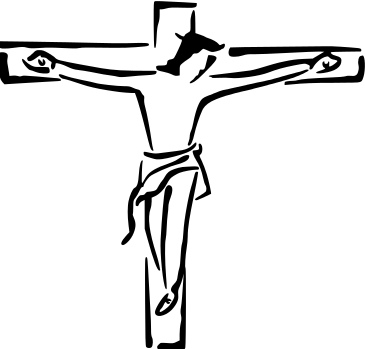
\includegraphics[width=0.20\textwidth]{../christ_on_cross.png}} ;
\end{tikzpicture}
\Large 

\leftcitation{ס} \centerfont 詩百又廿七載：
\leftcitation{ע} \centerfont 非耶和華建屋宇.則匠人之經營徒.
\leftcitation{פ} \centerfont 非耶和華衛城邑.則守者之儆醒徒.
\leftcitation{צ} \centerfont 余獻是卷予華人社區．願為福音流通之器．願獻斯微材為祭榮耀上帝．
\leftcitation{ק} \centerfont 阿門

\switchcolumn

\fontsize{11}{13}\rightfont \Large 滅．時越次聖殿期及當今。\leftcitation{י} \rightfont 猶太者力廣納之．筆錄以卷軸．便以傳、閱、頌、攜、守、鎖、抄、譯、釋、編，得書塔木德、密示拿等經傳．家喻戶曉．傳流若芳。\leftcitation{כ} \rightfont 猶太者文以載道．傳其口述．今我輩粵道之傳應當作如是．遂力行粵音識辨之法．載言載道．以盡忠傳粵道以待興。\leftcitation{ל} \rightfont 蒙下賜恩惠．無畏海量字音文書．既馭上帝之道．今廣及粵語講道．重駛編程之技．匯導粵音遂字稿．重塑講道現場．以傚猶太卷軸之舉便以傳流。\leftcitation{מ} \rightfont 是卷乃粵音口述傳之屬．莫通華文白話之語．

\end{paracol}

\columnratio{0.5,0.5}
\begin{paracol}{2}\fontsize{11}{13}\leftfont \Large \leftcitation{ו} \leftfont 斯殺一違儆百逆．既禁壓之．我輩聞風無奈．在所難免。\leftcitation{ז} \leftfont 另有異人例乎．以版權之名．脅網絡頻道之舉．同授礙予粵道之存流。

\switchcolumn

\fontsize{11}{13}\rightfont \Large 惟待後繼來者之傚．以譯釋傳之於神州華文地。\leftcitation{נ} \rightfont 今能排程驅馭圖靈以編彙文檔，其碼長共數千千亦無逢大礙．全蒙上帝保守。

\end{paracol}



\columnratio{1}\begin{paracol}{1}

\fontsize{11}{13}\rightfont \Large
~~~~~~~~~~~~~~~~~~~~~~~~~~~~~~~~~~~~~~~~~~~~~~~~~~~~~~~~~~~~~~~~~~~~~~~~~~~~~~~\leftcitation{ר} \rightfont 二零二三年二月一日

~~~~~~~~~~~~~~~~~~~~~~~~~~~~~~~~~~~~~~~~~~~~~~~~~~~~~~~~~~~~~~~~~~~~~~~~~~~~~~~\leftcitation{ש} \rightfont 米迦勒

~~~~~~~~~~~~~~~~~~~~~~~~~~~~~~~~~~~~~~~~~~~~~~~~~~~~~~~~~~~~~~~~~~~~~~~~~~~~~~~\leftcitation{ת} \rightfont 書於香港

\end{paracol}

\end{sloppypar}
\end{document}
